% Options for packages loaded elsewhere
\PassOptionsToPackage{unicode}{hyperref}
\PassOptionsToPackage{hyphens}{url}
%
\documentclass[
]{book}
\usepackage{amsmath,amssymb}
\usepackage{iftex}
\ifPDFTeX
  \usepackage[T1]{fontenc}
  \usepackage[utf8]{inputenc}
  \usepackage{textcomp} % provide euro and other symbols
\else % if luatex or xetex
  \usepackage{unicode-math} % this also loads fontspec
  \defaultfontfeatures{Scale=MatchLowercase}
  \defaultfontfeatures[\rmfamily]{Ligatures=TeX,Scale=1}
\fi
\usepackage{lmodern}
\ifPDFTeX\else
  % xetex/luatex font selection
\fi
% Use upquote if available, for straight quotes in verbatim environments
\IfFileExists{upquote.sty}{\usepackage{upquote}}{}
\IfFileExists{microtype.sty}{% use microtype if available
  \usepackage[]{microtype}
  \UseMicrotypeSet[protrusion]{basicmath} % disable protrusion for tt fonts
}{}
\makeatletter
\@ifundefined{KOMAClassName}{% if non-KOMA class
  \IfFileExists{parskip.sty}{%
    \usepackage{parskip}
  }{% else
    \setlength{\parindent}{0pt}
    \setlength{\parskip}{6pt plus 2pt minus 1pt}}
}{% if KOMA class
  \KOMAoptions{parskip=half}}
\makeatother
\usepackage{xcolor}
\usepackage{color}
\usepackage{fancyvrb}
\newcommand{\VerbBar}{|}
\newcommand{\VERB}{\Verb[commandchars=\\\{\}]}
\DefineVerbatimEnvironment{Highlighting}{Verbatim}{commandchars=\\\{\}}
% Add ',fontsize=\small' for more characters per line
\usepackage{framed}
\definecolor{shadecolor}{RGB}{248,248,248}
\newenvironment{Shaded}{\begin{snugshade}}{\end{snugshade}}
\newcommand{\AlertTok}[1]{\textcolor[rgb]{0.94,0.16,0.16}{#1}}
\newcommand{\AnnotationTok}[1]{\textcolor[rgb]{0.56,0.35,0.01}{\textbf{\textit{#1}}}}
\newcommand{\AttributeTok}[1]{\textcolor[rgb]{0.13,0.29,0.53}{#1}}
\newcommand{\BaseNTok}[1]{\textcolor[rgb]{0.00,0.00,0.81}{#1}}
\newcommand{\BuiltInTok}[1]{#1}
\newcommand{\CharTok}[1]{\textcolor[rgb]{0.31,0.60,0.02}{#1}}
\newcommand{\CommentTok}[1]{\textcolor[rgb]{0.56,0.35,0.01}{\textit{#1}}}
\newcommand{\CommentVarTok}[1]{\textcolor[rgb]{0.56,0.35,0.01}{\textbf{\textit{#1}}}}
\newcommand{\ConstantTok}[1]{\textcolor[rgb]{0.56,0.35,0.01}{#1}}
\newcommand{\ControlFlowTok}[1]{\textcolor[rgb]{0.13,0.29,0.53}{\textbf{#1}}}
\newcommand{\DataTypeTok}[1]{\textcolor[rgb]{0.13,0.29,0.53}{#1}}
\newcommand{\DecValTok}[1]{\textcolor[rgb]{0.00,0.00,0.81}{#1}}
\newcommand{\DocumentationTok}[1]{\textcolor[rgb]{0.56,0.35,0.01}{\textbf{\textit{#1}}}}
\newcommand{\ErrorTok}[1]{\textcolor[rgb]{0.64,0.00,0.00}{\textbf{#1}}}
\newcommand{\ExtensionTok}[1]{#1}
\newcommand{\FloatTok}[1]{\textcolor[rgb]{0.00,0.00,0.81}{#1}}
\newcommand{\FunctionTok}[1]{\textcolor[rgb]{0.13,0.29,0.53}{\textbf{#1}}}
\newcommand{\ImportTok}[1]{#1}
\newcommand{\InformationTok}[1]{\textcolor[rgb]{0.56,0.35,0.01}{\textbf{\textit{#1}}}}
\newcommand{\KeywordTok}[1]{\textcolor[rgb]{0.13,0.29,0.53}{\textbf{#1}}}
\newcommand{\NormalTok}[1]{#1}
\newcommand{\OperatorTok}[1]{\textcolor[rgb]{0.81,0.36,0.00}{\textbf{#1}}}
\newcommand{\OtherTok}[1]{\textcolor[rgb]{0.56,0.35,0.01}{#1}}
\newcommand{\PreprocessorTok}[1]{\textcolor[rgb]{0.56,0.35,0.01}{\textit{#1}}}
\newcommand{\RegionMarkerTok}[1]{#1}
\newcommand{\SpecialCharTok}[1]{\textcolor[rgb]{0.81,0.36,0.00}{\textbf{#1}}}
\newcommand{\SpecialStringTok}[1]{\textcolor[rgb]{0.31,0.60,0.02}{#1}}
\newcommand{\StringTok}[1]{\textcolor[rgb]{0.31,0.60,0.02}{#1}}
\newcommand{\VariableTok}[1]{\textcolor[rgb]{0.00,0.00,0.00}{#1}}
\newcommand{\VerbatimStringTok}[1]{\textcolor[rgb]{0.31,0.60,0.02}{#1}}
\newcommand{\WarningTok}[1]{\textcolor[rgb]{0.56,0.35,0.01}{\textbf{\textit{#1}}}}
\usepackage{longtable,booktabs,array}
\usepackage{calc} % for calculating minipage widths
% Correct order of tables after \paragraph or \subparagraph
\usepackage{etoolbox}
\makeatletter
\patchcmd\longtable{\par}{\if@noskipsec\mbox{}\fi\par}{}{}
\makeatother
% Allow footnotes in longtable head/foot
\IfFileExists{footnotehyper.sty}{\usepackage{footnotehyper}}{\usepackage{footnote}}
\makesavenoteenv{longtable}
\usepackage{graphicx}
\makeatletter
\def\maxwidth{\ifdim\Gin@nat@width>\linewidth\linewidth\else\Gin@nat@width\fi}
\def\maxheight{\ifdim\Gin@nat@height>\textheight\textheight\else\Gin@nat@height\fi}
\makeatother
% Scale images if necessary, so that they will not overflow the page
% margins by default, and it is still possible to overwrite the defaults
% using explicit options in \includegraphics[width, height, ...]{}
\setkeys{Gin}{width=\maxwidth,height=\maxheight,keepaspectratio}
% Set default figure placement to htbp
\makeatletter
\def\fps@figure{htbp}
\makeatother
\setlength{\emergencystretch}{3em} % prevent overfull lines
\providecommand{\tightlist}{%
  \setlength{\itemsep}{0pt}\setlength{\parskip}{0pt}}
\setcounter{secnumdepth}{5}
\usepackage{booktabs}
\usepackage{natbib}
\ifLuaTeX
  \usepackage{selnolig}  % disable illegal ligatures
\fi
\usepackage[]{natbib}
\bibliographystyle{plainnat}
\usepackage{bookmark}
\IfFileExists{xurl.sty}{\usepackage{xurl}}{} % add URL line breaks if available
\urlstyle{same}
\hypersetup{
  pdftitle={Geomatics for Environmental Management: An Open Textbook for Students and Practitioners},
  hidelinks,
  pdfcreator={LaTeX via pandoc}}

\title{Geomatics for Environmental Management: An Open Textbook for Students and Practitioners}
\author{}
\date{\vspace{-2.5em}}

\begin{document}
\maketitle

{
\setcounter{tocdepth}{1}
\tableofcontents
}
\chapter*{About this textbook}\label{about-this-textbook}
\addcontentsline{toc}{chapter}{About this textbook}

\begin{figure}
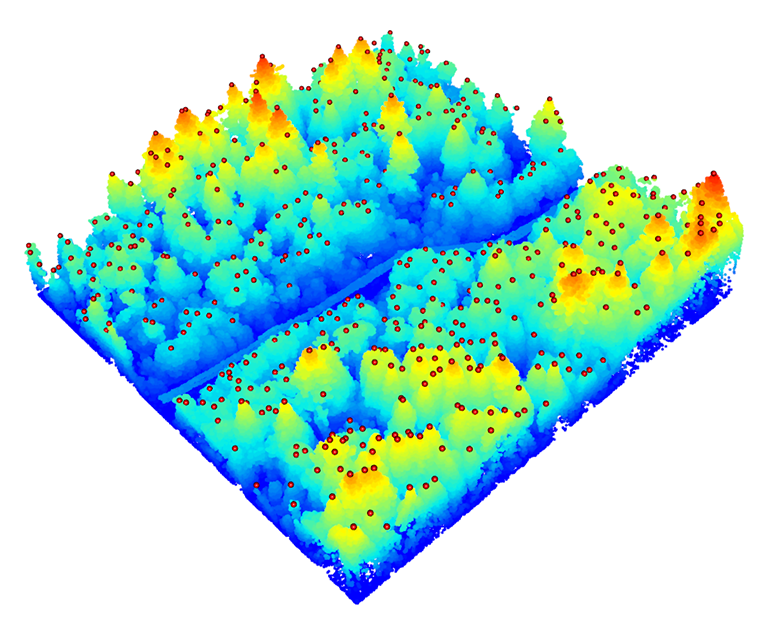
\includegraphics[width=0.75\linewidth]{images/15-las-treetops} \caption{Cover design by Du Toit, CC-BY-SA-4.0.}\label{fig:00-book-cover}
\end{figure}

Geomatics is a large and growing field that encompasses the art, science and technology of measuring attributes about Earth's systems. From the earliest observations of Earth's shape in ancient Greece to the space and information age, humans have wondered about their place on this planet. Nearly every aspect of our modern geographic lives can be attributed to advances in the field of geomatics. Today, location is real-time and precise, made easy by millennia of observations and incremental advances in technology that have culminated in a wondrous field of study.

The purpose of this textbook is to give students and practitioners a solid survey (pun intended) of what modern geomatics is capable of when confronting environmental management problems. We take a Canadian perspective to this approach, by telling the historical contributions of Canadians to the field and sharing real-world case studies of environmental management problems in Canada. Inside, you will find interactive web-based content and tools, case studies with real geographic data, and tons of reflection and practice questions. Best of all, unless otherwise stated, the content is free to use, adapt, and remix for any purpose with attribution to us and under the same \href{https://creativecommons.org/licenses/by-sa/4.0/}{Creative Commons 4.0 license}.

\section*{Who Should use this textbook}\label{who-should-use-this-textbook}
\addcontentsline{toc}{section}{Who Should use this textbook}

This textbook is designed to be used by students, instructors, and practitioners of geomatics. All the basics are covered for introducing Geographic Information Systems (GIS) and remote sensing at any level or as a refresher. We throw in a little extra for understanding common GIS workflows and some more advanced topics that are suitable for advanced students. Unlike many other geomatics textbooks, we do not adopt any specific GIS software and therefore any student or practitioner should be able pick up this textbook and apply the methods and knowledge to the software of your choice. That said, the textbook is created with many geospatial packages in R and because it is open, anyone is free to poke their head under the hood in the GitHub repository for specific workflows and geospatial data handling with R.

\section*{How to adopt this textbook in your geomatics classroom}\label{how-to-adopt-this-textbook-in-your-geomatics-classroom}
\addcontentsline{toc}{section}{How to adopt this textbook in your geomatics classroom}

Depending on what you are teaching and how you organize your course, you can easily assign readings that are thematic or sequential. A great way to get started with adopting this textbook is to read the clear and concise \textbf{Learning Objectives} that are displayed at the very beginning of each chapter and then compare with your own curriculum.

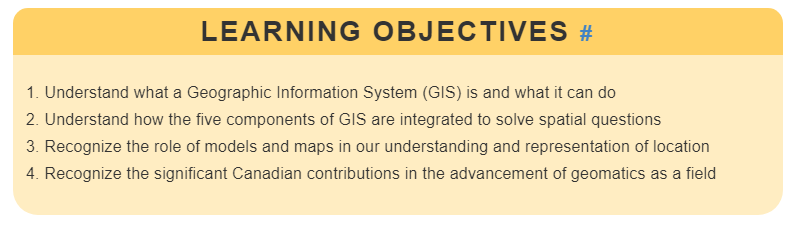
\includegraphics[width=0.75\linewidth]{images/00-learning-objectives}

Chapter 1 provides an overview of the field with some key definitions and a detailed history of much of the technology that is presented in later chapters. The remainder of the textbook can be divided into four parts:

\begin{itemize}
\tightlist
\item
  \textbf{Part 1} Chapters 2-5 cover \textbf{Geospatial Data Fundamentals} such as types of data, collecting and editing data, and relational database management systems.
\item
  \textbf{Part 2} Chapters 6-8 focus on \textbf{Spatial Analysis} and cover a wide variety of common workflows, some of which might be found in more advanced geomatics coursework like network analysis and spatial estimation.
\item
  \textbf{Part 3} Chapters 9-13 focus on everything \textbf{Remote Sensing} including theory, systems, image processing and analysis, Global Navigation Satellite Systems, and LiDAR (light detection and ranging).
\end{itemize}

Chapters are written to stand alone as authoritative contributions on specific topics, but an accumulative approach is taken to content organization. In this way, the textbook can be adopted in sequence as-is for an entire semester or you can adopt the chapters that suit the needs for your course and compliment them with other materials. Each chapter is also subdivided into subsections that can be easily linked to for an assigned reading.

\section*{How to get involved}\label{how-to-get-involved}
\addcontentsline{toc}{section}{How to get involved}

Because this is an open project, we highly encourage contributions from the community through our \textbf{Open Geomatics Community of Practice} on GitHub. The textbook is hosted on our GitHub repository and from there you can open an issue or start a discussion. Feel free to open an issue for any typos, factual discrepancies, bugs, or topics you want to see in a future edition. We are always looking for great Canadian case studies to share! Beyond the built versions of the textbook (e.g., \href{http://www.opengeomatics.ca}{www.opengeomatics.ca}, pdf, epub, etc.), you can fork our GitHub repository to explore the source code.

\section*{Acknowledgements}\label{acknowledgements}
\addcontentsline{toc}{section}{Acknowledgements}

So many folks helped with the development of this textbook and many of them are named as authors in various chapters. For those not explicitly named with contributions, we greatly thank the efforts by Nick Murphy for collating our bibliographic sources, Natasha Sharma for editing and fixing things, students enrolled in the Master of Geomatics for Environmental Management program at the University of British Columbia for contributing case studies and early reviews. This textbook would not have been possible without the support of an Open Educational Resources (OER) Implementation Grant from the University of British Columbia.

\chapter{What is Geomatics?}\label{what-is-geomatics}

Written by
Paul Pickell

We encounter and use geographic information on a regular basis in our everyday lives. Whether it is finding directions to a retailer that has an item in stock you want to buy or recording the path of your last morning jog, you have probably used a Geographic Information System (GIS) and not even realized it. In this chapter, we explore what geomatics is all about.

\section*{Learning Objectives}\label{learning-objectives}
\addcontentsline{toc}{section}{Learning Objectives}

\begin{enumerate}
\def\labelenumi{\arabic{enumi}.}
\tightlist
\item
  Understand what a Geographic Information System (GIS) is and what it can do
\item
  Understand how the five components of GIS are integrated to solve spatial questions
\item
  Recognize the role of models and maps in our understanding and representation of location
\item
  Recognize the significant Canadian contributions in the advancement of geomatics as a field
\end{enumerate}

\section*{Key Terms}\label{key-terms}
\addcontentsline{toc}{section}{Key Terms}

Attributes, Canada Geographic Information System, Conceptual Model, Data Model, Geomatics, Geographic Information Systems (GIS), Map, Model, Photogrammetry, Remote Sensing, Trimetrogon

\section{The Science and Technology of Geomatics}\label{the-science-and-technology-of-geomatics}

\textbf{Geomatics} is the science and technology of collecting geographic data and converting it to geographic information for use in a wide variety of industries. As a technical field, it encompasses many different work processes including surveying, remote sensing, global navigation satellite systems, geospatial analysis, and information technology and systems management. In turn, these processes support a wide variety of spatial decision-making such as urban planning, ecological conservation, forest management, real-time planetary systems monitoring, and rapid response to natural disasters. Many more emerging technologies such as self-driving vehicles, ride-sharing apps, and augmented reality video games depend directly on the science and technology of geomatics.

\section{Information Systems}\label{information-systems}

An \textbf{information system} is used to store, code, and recall information. In the Information Age, we are surrounded and depend heavily on information systems such as financial systems that record the transactions in your bank account or navigation systems that tell you the fastest route to a destination or autonomous vehicles such as the SkyTrain rapid transit network in Vancouver, Canada that moves more than a half million people every day across the Metro Vancouver region. These are all examples of systems that require high synchronization and integration of many varied sources of information in order to move people and assets around. It should come as no surprise then that information systems and information technology contribute significantly to nearly every sector of developed and developing economies.

What makes a \textbf{Geographic Information System} different from other information systems is the type of information that is handled: geographic location. With a GIS you can know the quantity and quality of something and the \emph{location} of that event, activity, or feature. For example, you might have recorded your heart rate and timed your morning jog using your phone or other fitness tracking device. Since you also have the location or coordinates of your jog, you can calculate or derive additional information such as speed (distance per time), the total distance you jogged, and also your elevation above sea level. You could even relate your heart rate to different locations along your jog to better understand your performance on different terrain. This is an example of a GIS at work. You are storing geographic information into a system that allows you to code the information with different qualities (e.g., the type of surface your ran on) and quantities (e.g., your heart rate) and then recall that information in a way that allows you to explore trends and ask and answer \emph{spatial} questions.

\section{The Five Components of GIS}\label{the-five-components-of-gis}

A GIS is a collection of five inter-connected, inter-acting, and inter-dependent components (Figure \ref{fig:1-five-components-gis}).

\begin{figure}
\includegraphics[width=0.75\linewidth]{images/01-five-components-gis} \caption{The five components of a geographic information system. Pickell, CC-BY-SA-4.0.}\label{fig:1-five-components-gis}
\end{figure}

\textbf{Data} -- Data are a collection of qualitative and quantitative variables about real world entities. At the very least, the type of data stored in a GIS is usually spatial in nature, meaning we have some set of coordinates or representation of location. But a GIS can also store aspatial data, data that does not necessarily have coordinates, but may still be relevant to other geographic data For example, you might also record the dates that you jogged or the weather during your jogs. These are examples of aspatial information that we might want to relate to your jogs.

\begin{figure}
\includegraphics[width=0.75\linewidth]{images/01-jogging-path} \caption{Abstracted spatial and aspatial information from a jogging path represented by three ordered points. Pickell, CC-BY-SA-4.0.}\label{fig:1-jogging-path}
\end{figure}

Spatial data can take many forms in a GIS. For the sake of our jogging example, you can imagine your jogging path could be represented as a line or a set of ordered points. In turn, your jogging path can be described by different qualities (day of the week, weather) and quantities (distance, speed, heart rate), which are called \textbf{attributes} (Figure \ref{fig:1-jogging-path}). An important role of a GIS is to govern how data can interact and behave with other types of data. For example, we can calculate distance from a line, but not area, which is a special property of a polygon.

\textbf{Software} -- There are a lot of different GIS software packages available and the choice of which software to use is usually driven by preference, availability, and/or cost. For example, some GIS software are freely available while others require a paid license. Nearly all GIS software packages can perform the same operations and analyses, but there are some differences like integrated cloud computing or availability of certain plugins. The most widely-used paid software is ESRI's ArcGIS, while the most widely-used Free and Open Source Software (FOSS) is QGIS (Q for Quantum). There are many other historically-significant FOSS software packages like GRASS, SAGA, and MOSS that are discussed in more detail later in this chapter.

\textbf{Hardware} -- GIS software operate on hardware comprised of computer components and human interface devices (HID). High resolution and high refresh rate monitors are often required when dealing with high resolution imaging and other digitizing, which require high-end graphics cards. Solid State Disks (SSD) with high capacity are important for fast read-write speeds to access and process data while Random Access Memory (RAM) and Central Processing Unit (CPU) clock speed can also be limiting factors for processing. Some specialized HID are designed specifically for working with GIS such as active shutter and polarized glasses for stereo vision, and joysticks for navigating in 3D space.

\textbf{Methods} -- All organizations must design business processes in order to effectively operationalize GIS for solving real-world problems. Methods will vary from organization to organization based on industry, client needs, and the types of data needed. For example, the business process of a forestry company will involve digitizing forest stands and other natural resources, enumerating attributes for stand inventories, road and forest harvest planning, forest regeneration monitoring, and creating operational maps. It is important for an organization to define exactly the activities, standards, and quality assurance (i.e., methods) that will be needed to achieve operational goals. Well-defined and well-documented methods also ensure that organizational knowledge is retained during staff turnover.

\textbf{People} -- We are responsible for identifying the information needs, defining the procedures, coding the software, and building the hardware for a Geographic Information System. We are also responsible for interpreting, analysing, and reporting our results and communicating our findings through maps and reports. Geographic Information Systems do not occur naturally and because they are a product of our imagination and skill, they inherit our best and worst traits. For example, we often make mistakes when we define our procedures or identify our information needs, which lead to incorrect conclusions. Moreover, our biases intentionally and unintentionally creep into our map-making, distorting shape, size, and importance of features that we want to represent.

\section{What a GIS can do}\label{what-a-gis-can-do}

Like other information systems, a GIS should be able to do the following things with geospatial data:

\begin{itemize}
\tightlist
\item
  Capture geospatial data
\item
  Store geospatial data
\item
  Query geospatial data
\item
  Analyse geospatial data
\item
  Display geospatial data
\item
  Output geospatial data
\end{itemize}

Geospatial data may be \textbf{captured} from remote sensing or digitized/scanned from other sources. Data can be \textbf{stored} in many different formats with different behaviours and rules and are kept in databases. Data can be queried (or selected) from a database using a standard query language. Once data are queried, they can then be \textbf{analysed} using operations like proximity, overlay, intersection and zonal statistics. A primary justification for investing resources into a GIS is to display and \textbf{output} data in the form of graphs, tables, charts, and maps.

A GIS ultimately answers spatial questions like:

\begin{itemize}
\tightlist
\item
  Where should I buy a home?
\item
  Where is population density highest in Vancouver, Canada?
\item
  Where is the most economical location for a new mill?
\item
  Where should land be protected or conserved?
\end{itemize}

\section{Modelling the world with GIS}\label{modelling-the-world-with-gis}

Together, the five components of a GIS allow us to model our spatial environment. A \textbf{model} is an abstraction or simplification of reality. Models are necessary for us to understand how complex things work and communicate that understanding to others. For example, the hydrologic cycle describes the states and processes of water in the atmosphere, over land, in the ocean as well as forms of precipitation and evaporation. The concept of the hydrologic cycle is a simplification, of course, because movement and the phase of water is caused by all kinds of interacting forces such as gravity, temperature, pressure, and climate. For this reason, the hydrologic cycle is an example of a \textbf{conceptual model}, which is used to hypothesize and theorize about how our world works. This brings us to the second important quality of models: they are reproducible. A model must be reproducible so that we can validate it or check that the result or output is in line with what we expect or observe. For example, the principles of the hydrologic cycle are universal, that is they apply anywhere on Earth and even on other planets because they are based on physical properties that are shared across our universe (e.g., temperature, pressure, gravity).

We can also create models that allow us to play out different scenarios and assess the possible range of outcomes in geographic space. For example, you might be interested in purchasing a home, but you have some spatial and aspatial criteria such as price range, preference of neighborhood, distance to your work, or the quality of the nearby schools. This is the type of spatial optimization problem that we often seek to solve with a GIS. If you go onto a property listing website, you will notice that the results will change based on the criteria that you enter. And this brings us to the final type of model that is important to a GIS: the map.

\section{Technology}\label{technology}

Modern GIS cannot be understood without the context of three majors technological leaps in the nineteenth and twentieth centuries: the photograph, the airplane, and the computer. None of these technologies were discovered by Canadians, yet all were instrumental for the Canadian cartographic advances that followed.

\subsection{The Photograph}\label{the-photograph}

The first successful attempt to record light on a durable image can be traced to France. Nicéphore Niépce is widely credited with the invention of photography by producing the oldest surviving photograph from the window of his home in 1826 or 1827 simply titled, \emph{View from the Window at Le Gras} (Figure \ref{fig:1-View-from-the-Window-at-Le-Gras}). His process involved using a camera obscura (a discovery handed down from antiquity) to project a real-world scene onto a photosensitive metal plate for hours and possibly days on end. Though the results were crude, it was a major advancement over all earlier attempts that failed to produce a durable photograph. Niépce died only a few years later in 1833 before he was able to publish his invention. Before his death, he shared his secrets with Louis Daguerre who would perfect his process and announce the daguerreotype to the world in 1839, a photographic process that was much faster and commercially viable. The announcement of the daguerreotype from France spread rapidly and resulted in the first known photograph captured of Canada the very next year of Niagara Falls, Ontario (Figure \ref{fig:1-niagara-falls-daguerreotype-1840}).

\begin{figure}
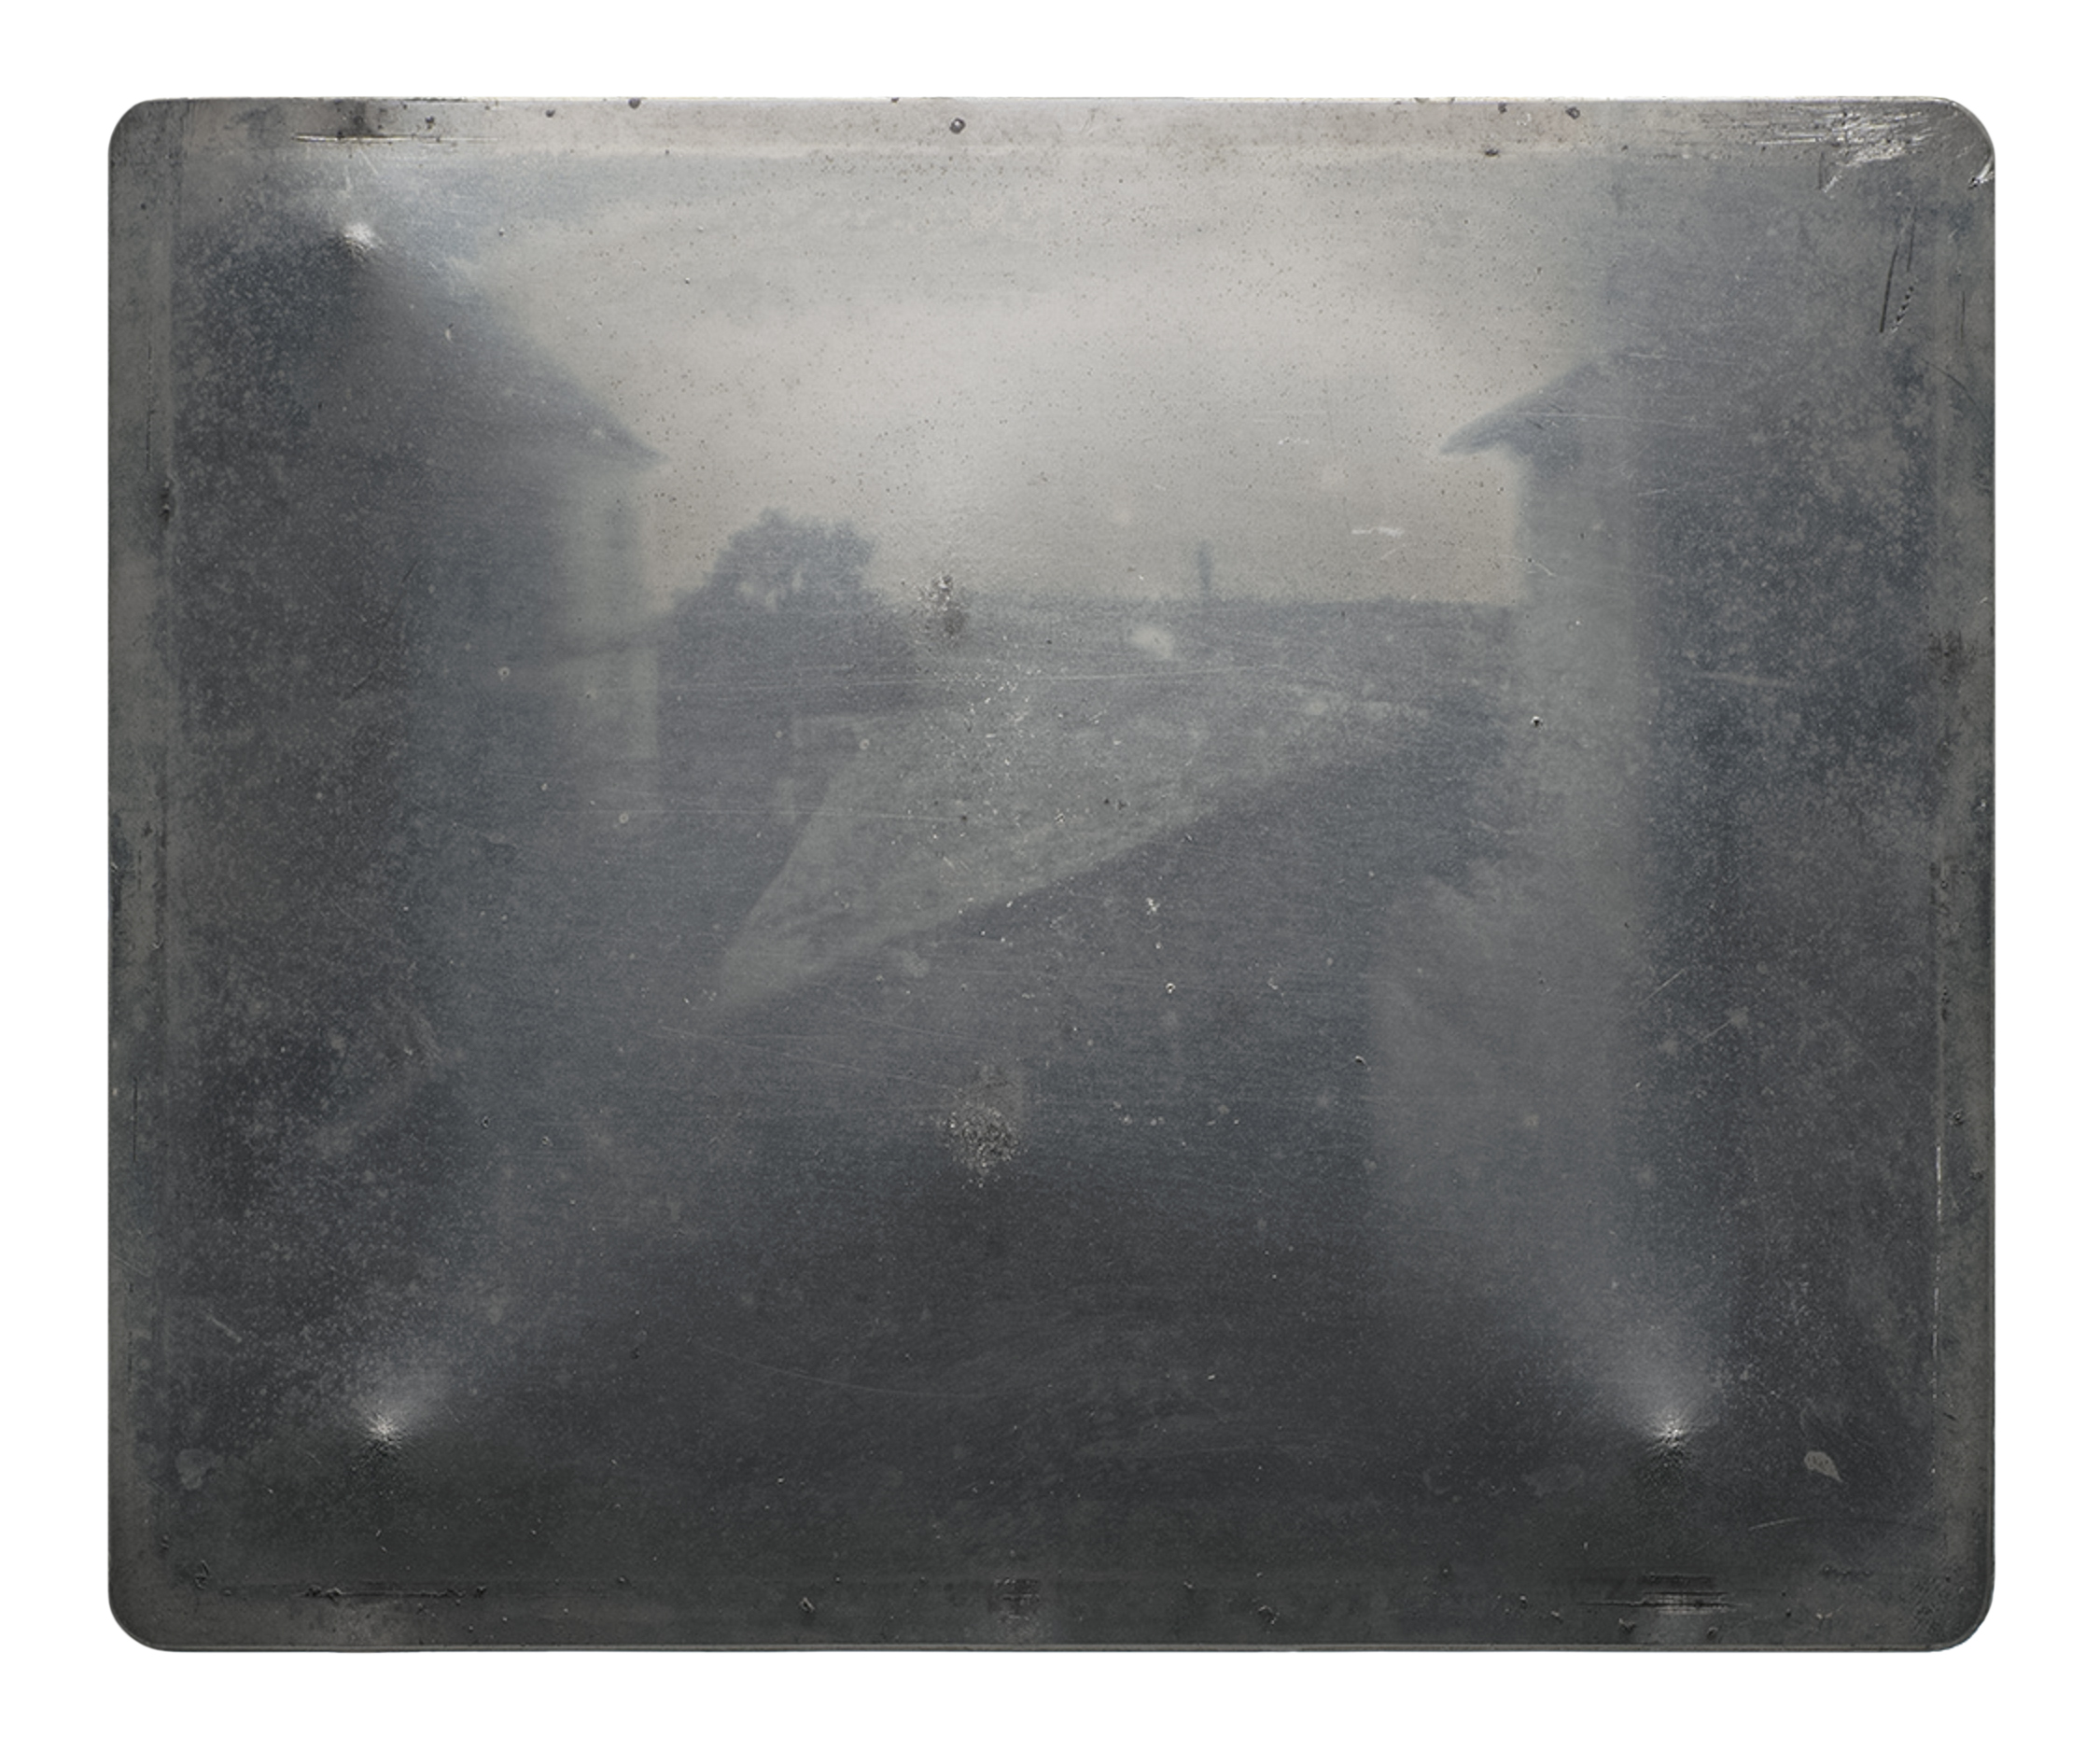
\includegraphics[width=0.75\linewidth]{images/01-View-from-the-Window-at-Le-Gras} \caption{View from the Window at Le Gras showing some buildings and a tree in the distance. This image has been flipped from the original metal plate along both the horizontal and vertical axes. The camera obscura would have originally recorded the upper right corner in the lower left corner. Public Domain.}\label{fig:1-View-from-the-Window-at-Le-Gras}
\end{figure}

\begin{figure}
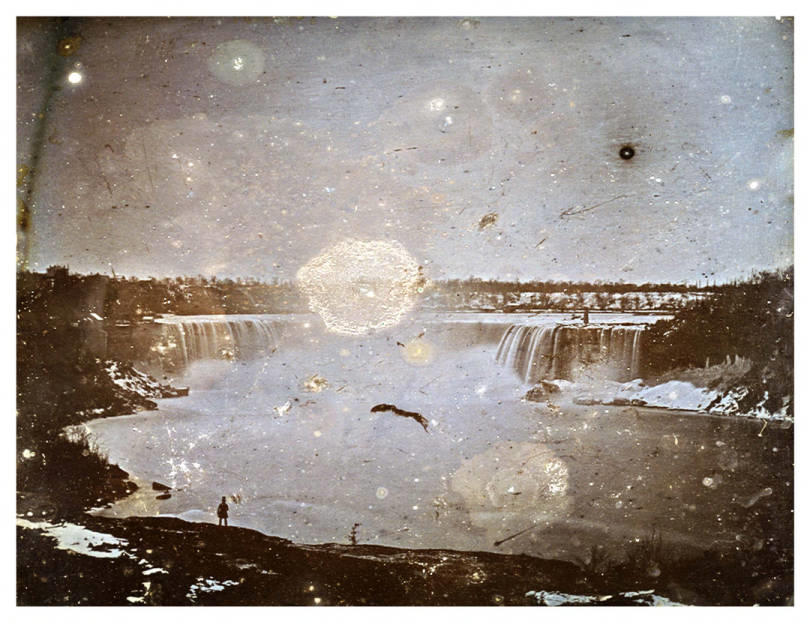
\includegraphics[width=0.75\linewidth]{images/01-niagara-falls-daguerreotype-1840} \caption{The earliest known photograph of present-day Canada was this daguerreotype taken in 1840 by Hugh Lee Pattinson of Niagara Falls, Ontario (Horseshoe Falls). Due to the dagguerrotype capture process, the image is flipped on the vertical axis so that image right is the United States on the East side of the falls and image left is Canada on the West side of the falls (image is looking South). Courtesy of Newcastle University Library Special Collections, CC-BY-SA-4.0}\label{fig:1-niagara-falls-daguerreotype-1840}
\end{figure}

It was not long before more Canadian landscapes became the subjects of photography. In the next decade, French colonel Aimé Laussedat developed a new instrument that combined a contemporaneous camera with a theolodite (a surveying instrument) that he called a phototheodolite. The phototheodolite allowed photographs to be precisely taken such that multiple photographs could provide various perspectives of known locations in order to produce topographic maps. By 1867, Laussedat exhibited the first map of Paris produced with a phototheodolite and in doing so he ushered in the field of \textbf{photogrammetry}, the science of deriving 3D measurements from 2D photographs. In 1887, the Geological Survey of Canada set out to photograph the Rocky Mountains using these photogrammetric techniques and the Canadian Rockies became one of the most photographed landscapes of the day with over 25,000 historical images captured between 1887 and 1958. Today, these historical images have been digitised from Library and Archives Canada through the \href{http://mountainlegacy.ca/}{Mountain Legacy Project} and many locations have been re-imaged more than a century later by researchers at the University of Alberta and University of Victoria, illuminating dramatic changes to glaciers and forest cover on these Canadian landscapes.

\subsection{The Airplane}\label{the-airplane}

The next technological leap came at the turn of the century and forever transformed photography and photogrammetry. From 1900 to 1902, Orville and Wilbur Wright had been designing and experimenting with light-than-air gliders and kites near Kitty Hawk, North Carolina. By 1903, the brothers had designed the first heavier-than-air airplane capable of powered flight by a gasoline engine called the \emph{Wright Flyer}. Incidentally, because the technology of photography had developed six decades earlier, the moment of this first flight was captured in one of the most iconic photographs ever taken by John T. Daniels, member of the U.S. Lifesaving Service Station at Kill Devil Hills who was standing by (Figure \ref{fig:1-wright-flyer}).

\begin{figure}
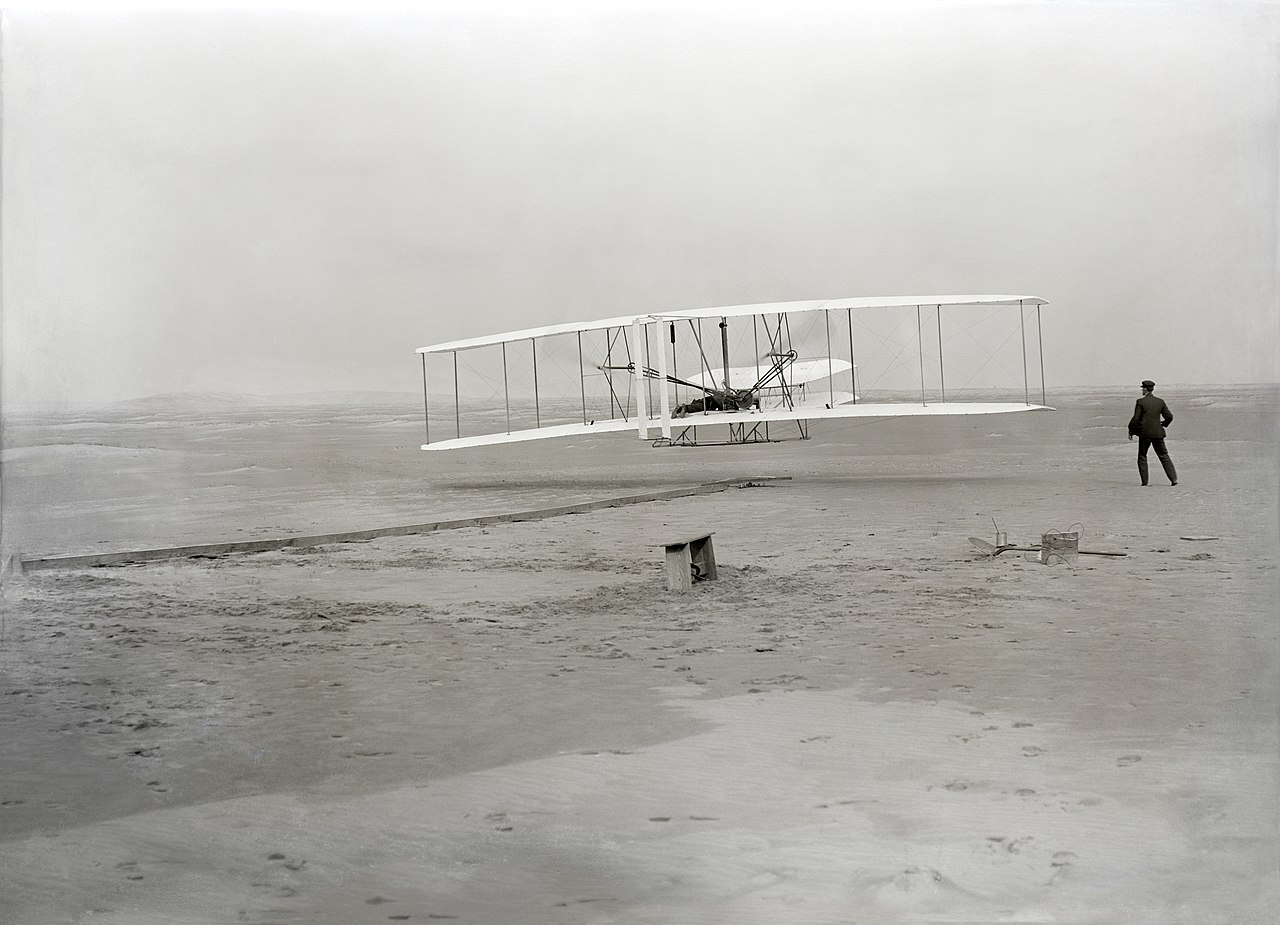
\includegraphics[width=0.75\linewidth]{images/01-wright-flyer} \caption{Restored image taken by John T. Daniels on December 17, 1903 near Kitty Hawk, North Carolina only seconds into the 12 second first powered flight piloted by Orville Wright. Wilbur Wright is seen to the right. Public Domain.}\label{fig:1-wright-flyer}
\end{figure}

Aviation developed quickly following the first successful powered flight by the Wright Brothers and so did aerial photography. In 1912, Frederick Charles Victor Laws of the British Royal Flying Corps discovered that aerial photographs taken with at least 60\% overlap could be used to produce a 3D stereographic effect when viewed through a \textbf{stereoscope} (Figure \ref{fig:1-woman-stereoscope}). Following Laws' realization, flight paths were more intentionally planned to achieve this effect and in the coming years many more personnel were employed to help with \textbf{air photo interpretation}, the process of viewing air photos and discerning types of features based on tone, shade, shape, pattern, texture, and spatial association. At the outset of World War I, aircraft were being equipped with cameras for reconnaissance at the front lines.

\begin{figure}
\includegraphics[width=0.75\linewidth]{images/01-woman-stereoscope} \caption{A woman is seen annotating an overlapping air photo pair with a stereoscope in 1945. Canada. Dept. of National Defence / Library and Archives Canada / PA-065599, Public Domain.}\label{fig:1-woman-stereoscope}
\end{figure}

The Canadian government quickly realized the potential benefits of air travel and aerial surveying for such a large country. In 1919, Canada became the first nation to regulate the domain of aviation with the establishment of the Air Board. Six air stations were established by the Air Board around the country primarily for civil patrols and surveying (Figure \ref{fig:1-jericho-air-station}). By 1922, Canada established the National Air Photo Library to store the new and increasing cache of air photos being collected by federal agencies. During the 1930's, many private companies began prospecting from the sky and found profit in undertaking aerial mineral surveys in the Northwest Territories and the Yukon.

\begin{figure}
\includegraphics[width=0.75\linewidth]{images/01-jericho-air-station} \caption{One of the first air stations established after the inception of the Air Board was Jericho Air Station seen here in 1923 near Vancouver, Canada. Canada. Dept. of National Defence / Library and Archives Canada / PA-051943, Public Domain.}\label{fig:1-jericho-air-station}
\end{figure}

Airplanes played a more significant role in World War II both as weapons and for reconnaissance. A new process for collecting aerial imagery was developed called \textbf{trimetrogon}, which involves capturing three photos at the same time: one directly down and two oblique images to the right and left of the airplane (Figure \ref{fig:1-trimetrogon-airplane}). Even in the 1940's, much of Canada remained unmapped and unimaged, so the Royal Canadian Air Force contributed multiple photo squadrons with the task of mapping the vast country. One of those squadrons was No.~413 Photographic Squadron (Figure \ref{fig:1-no-413-squadron}), which was based out of Canadian Forces Base Rockcliffe near Ottawa (formerly Rockliffe Air Station, the first air station established in Canada) and responsible for capturing the first aerial images of northern Canada. In the summer of 1950, No.~413 Photographic Squadron completed imaging the last gaps of land near Ellsemere Island. For the first time ever and more than 30 years after aerial surveys began, Canada finally had a self portrait from the sky. Today, a century after aerial surveying efforts began, the National Air Photo Library archives over six million air photos.

\begin{figure}
\includegraphics[width=0.75\linewidth]{images/01-trimetrogon-airplane} \caption{Trimetrogon camera installation in North American "Mitchell" II aircraft of No. 14 Photo Squadron, Royal Canadian Air Force seen in 1945. One of the oblique angle cameras can be seen on the side of the aircraft toward the nose. Library and Archives Canada / PA-065503, Public Domain.}\label{fig:1-trimetrogon-airplane}
\end{figure}

\begin{figure}
\includegraphics[width=0.75\linewidth]{images/01-no-413-squadron} \caption{Inside the fuselage of an aircraft of RCAF No. 413 Squadron showing an alternative arrangement of trimetrogon cameras with the oblique cameras pointing inward instead of outward. Library and Archives Canada / PA-065920, Public Domain.}\label{fig:1-no-413-squadron}
\end{figure}

After World War II, many RCAF pilots went on to start their own aerial surveying companies and benefited from the immense mapping efforts that were underway across the nation. One particular company, Spartan Air Services, emerged in 1946. Founded by two retired RCAF pilots, Spartan Air Services was based in Ottawa and undertook aerial mapping and surveying around the world. It was a chance encounter with an air photo interpreter from Spartan Air Services that would inevitably redefine how maps were created.

\subsection{The Computer}\label{the-computer}

Computers are central to geomatics because they provide the hardware and software components of a geographic information system. As they relate to geomatics, computers need to be understood in two different contexts: navigation and machines.

The word ``computer'' derives from the latin verb \textbf{putare}, which means to think and prune. Curiously, this inconspicuous latin verb is found as the root of many other words that include thinking and simplifying such as ``computation'', ``reputation'', and ``disputation'' to name a few. However it came about, ``computing'' was synonymous with ``reckoning'' as early as the seventeenth century, which was essentially to count or calculate something. For navigators of the day, one of the most perplexing computational problems was known as the \textbf{longitude problem}, which simply involved estimating east-west location (i.e., longitude) at sea, something that today is made trivial by satellites orbiting high above Earth. While latitude (i.e., north-south location) can be easily computed from a reference point like the the elevation of Polaris (the North Star) above the horizon during a clear night in the northern hemisphere or the elevation of the Sun above the horizon during the day, computing longitude astronomically is complicated by the fact that these celestial bodies are whizzing by in the same direction (west-to-east) that the Earth is rotating, so there is no fixed reference point to measure from.

For centuries, seafarers used a method known as ``dead reckoning'', which is basically a computation of speed and direction to estimate a new location from a reference location with a known longitude, like a port city. While direction could be known from a compass, the problem with this method was the inaccuracy for estimating speed on board a ship. The ``dead'' in ``dead reckoning'' is believed to originate from the method of tossing a log attached to a measured line overboard---considered ``dead'' in the water---and counting the time for the rope to outstretch using an hour glass. It was the best method of the day, but resulted in many shipwrecks due to incorrect ``reckoning''. Ultimately, the Parliament of Great Britain passed the Longitude Act of 1714, which established the Longitude Board and a prize for anyone who could solve this problem at sea.

A curious fact about Earth that offers a taunting solution is that the Earth's rotational period of 24 hours divided by 360 degrees found in a circle yields 15 degrees of longitude per hour or 0.25 degrees per minute. Therefore, if you know your local time and compared it with the time of the port that you want to arrive at, then you would know how far east or west you are from that port by simply multiplying the hour time difference by 15 degrees. This is, in fact, how Greenwich, England became the site of the Royal Observatory, the Prime Meridian we use today (0 degrees longitude), and Greenwich Mean Time (GMT). Local Mean Time (LMT) is the local time based on the average length of a solar day. Therefore, all locations along any meridian of longitude share the same LMT. As a simple example, if Vancouver is at -123.116226° west longitude and GMT is currently 1 PM (13:00) then Vancouver's LMT is \(-123.116226÷15+13=4.7922516\) or about 4:54 AM. Thus, time and longitude are one and the same.

However, errors compound and this method could be as deadly as dead reckoning because for every second that your time piece is off, your estimated location on Earth drifts about half a kilometer at the Equator (distance between lines of longitude are greatest at the Equator and shrink to zero at the poles). Dava Sobel writes in her history of the longtiude problem \textbf{Longitude: The True Story of a Lone Genius Who Solved the Greatest Scientific Problem of His Time} that the best pendulum time pieces in the mid-seventeenth century, known then as chronometers, lost about 10 seconds each day, which would amount to 1.25° of error in longitude over a 30 day voyage or 139 km at the Equator. Other factors such as temperature changes, constant winding, and the rolling of ship decks plagued the ability for chronometers to maintain the time. Many astronomical solutions were also proposed. For example, Galileo discovered from his observations that Jupiter's four brightest moons were eclipsed by the gas giant at regular intervals and that this phenomenon could be used to tell time anywhere. This discovery proved much more challenging to apply at sea, with crude telescopes of the day on a moving ship. Ultimately, it was the carpenter-turned-clock-maker John Harrison who built the first sea-worthy-chronometer and claimed the prize money from the Longitude Board over a period of 36 years for solving the longitude problem. In Harrison's day, a ``computer'' literally described a person or more accurately a person's job, whose responsibility was to reckon or calculate.

In the modern era, the word ``computer'' refers to a machine, not unlike the chronometers that came under trial to solve the longitude problem. The first transistor computer that resembles the technology we use today was built by Bell Labs in 1954. Up through the 1970s, the word ``computer'' continued to refer to a profession, one that was frequently held by women. Computers today are the machines that perform the necessary calculations that make geomatics look effortless. Behind the screens, literally billions of calculations per second are occuring when you capture, store, query, analyse, display, and output geospatial data. GIS software increasingly demands more computing power as new features and functionality are added. While a lot of geomatics is still done on desktops, more and more computing is now happening in the cloud with services like Google Earth Engine providing the ability to analyse petabytes (1 PB = 1,024 TB = 1 million GB) of remotely sensed imagery through a web browser.

\section{The Land Use Problem in Canada}\label{the-land-use-problem-in-canada}

The technologies of the photograph, the airplane, and the computer collided suddenly in the 1960s in Canada and evolved into the GIS that we know today.

The post-war economy of Canada saw significant growth in the 1940s and 1950s and huge demographic shifts were underway. Agrarian societies were transformed by the new economy and rapid urbanization. Prior to the Second World War, about half of all Canadians lived in rural areas. By the 1950s, nearly 62\% of the total population lived in urban centres and 37\% lived in just the fifteen largest cities (Figure \ref{fig:1-ninth-census-1951-map}). Faced with the prospect of failed crops and uncertain economic outcomes, many chose to head for better opportunities promised in the metropolitan areas. In the decade from 1941 to 1951, 105 Canadian families left their farms every week, despite an overall increase in farmland across the country \citep{dominion_bureau_of_statistics_volume_1944} \citep{dominion_bureau_of_statistics_number_1952}.

\begin{figure}
\includegraphics[width=0.75\linewidth]{images/01-ninth-census-1951-map} \caption{Ninth Census of Canada 1951, Population Distribution. Dominion of Bureau Statistics, Public Domain.}\label{fig:1-ninth-census-1951-map}
\end{figure}

As cities sprawled, land use and land planning conflicts emerged. City waistlines grew as adjacent farmland was consumed to welcome new urban dwellers. In 1957, the Senate established the Special Committee on Land Use in Canada whose purpose was ``to consider and report on land use in Canada and what should be done to ensure that our land resources are most effectively utilized for the benefit of the Canadian economy and the Canadian people and, in particular, to increase both agricultural production and the incomes of those engaged in it'' \citep{the_senate_of_canada_minutes_1957}. Over the next four years, the special committee heard testimony from 109 witnesses and recorded 1,606 pages of evidence on the issue of land use in Canada \citep{special_committee_on_land_use_in_canada_consolidation_1963}.

Following years of hearings by the Senate Special Committee on Land Use in Canada, the Agricultural and Rural Development Act was passed by Parliament in June 1961 \citep{mccrorie_arda_1969}. The new legislation empowered the Minister of Agriculture to work with the Provinces and Territories to address rural poverty and promote the development and conservation of Canada's prized farmland. By October, the federal government had organized a national conference in Montreal, ``The Resources for Tomorrow''. Over 700 delegates from government, non-governmental organizations, university, and industry contributed to a unique national conversation on the future of Canada's renewable natural resources with workshops on agriculture, forestry, fisheries, recreation, wildlife, water and urban growth \citep{gray_resources_1962}. The conference was attended by then Governor General Georges Philias Vanier, Prime Minister Diefenbaker, and future Prime Minister Pierre Elliot Trudeau.

In the following year, Rachel Carson published her landmark \emph{Silent Spring}. The publication catalysed public sentiment for protecting people and the environment from harmful pesticide and herbicide use. It was clear that a national approach to mapping renewable resources was needed in order to protect and conserve them, so in 1963 the federal government established an ambitious project called the Canada Land Inventory whose chief purpose was to provide a ``comprehensive survey of land capability and use designed to provide a basis for resource and land use planning'' \citep{department_of_regional_economic_expansion_canada_1965}.

But how could the Canada Land Inventory ever be achieved for such a vast country using traditional paper maps? To be sure, Canada was not lacking the mapped data. In fact there were tens of thousands of maps produced, cataloged, and housed by the federal government on everything from soils to agriculture to recreation to forests. Still, the scale of agricultural land loss was not known at the time because paper maps of soil fertility could not easily be combined with other information like census data. Decision-makers relied on human interpretation and analysis of paper maps, a time-consuming task that could only accommodate a handful of mapped attributes at a time over a small area. Paper maps had to be reproduced at the same scale, aligned, and analysed polygon-by-polygon. The process to create maps at the time was entirely manual, requiring approximately 10 hours by a skilled technician to produce a single map sheet and about as much time by another to check and make any corrections \citep{tomlinson_application_1974}. At that rate, it would have taken a A new approach was needed to cope with the overwhelming amount of information being produced.

\begin{figure}
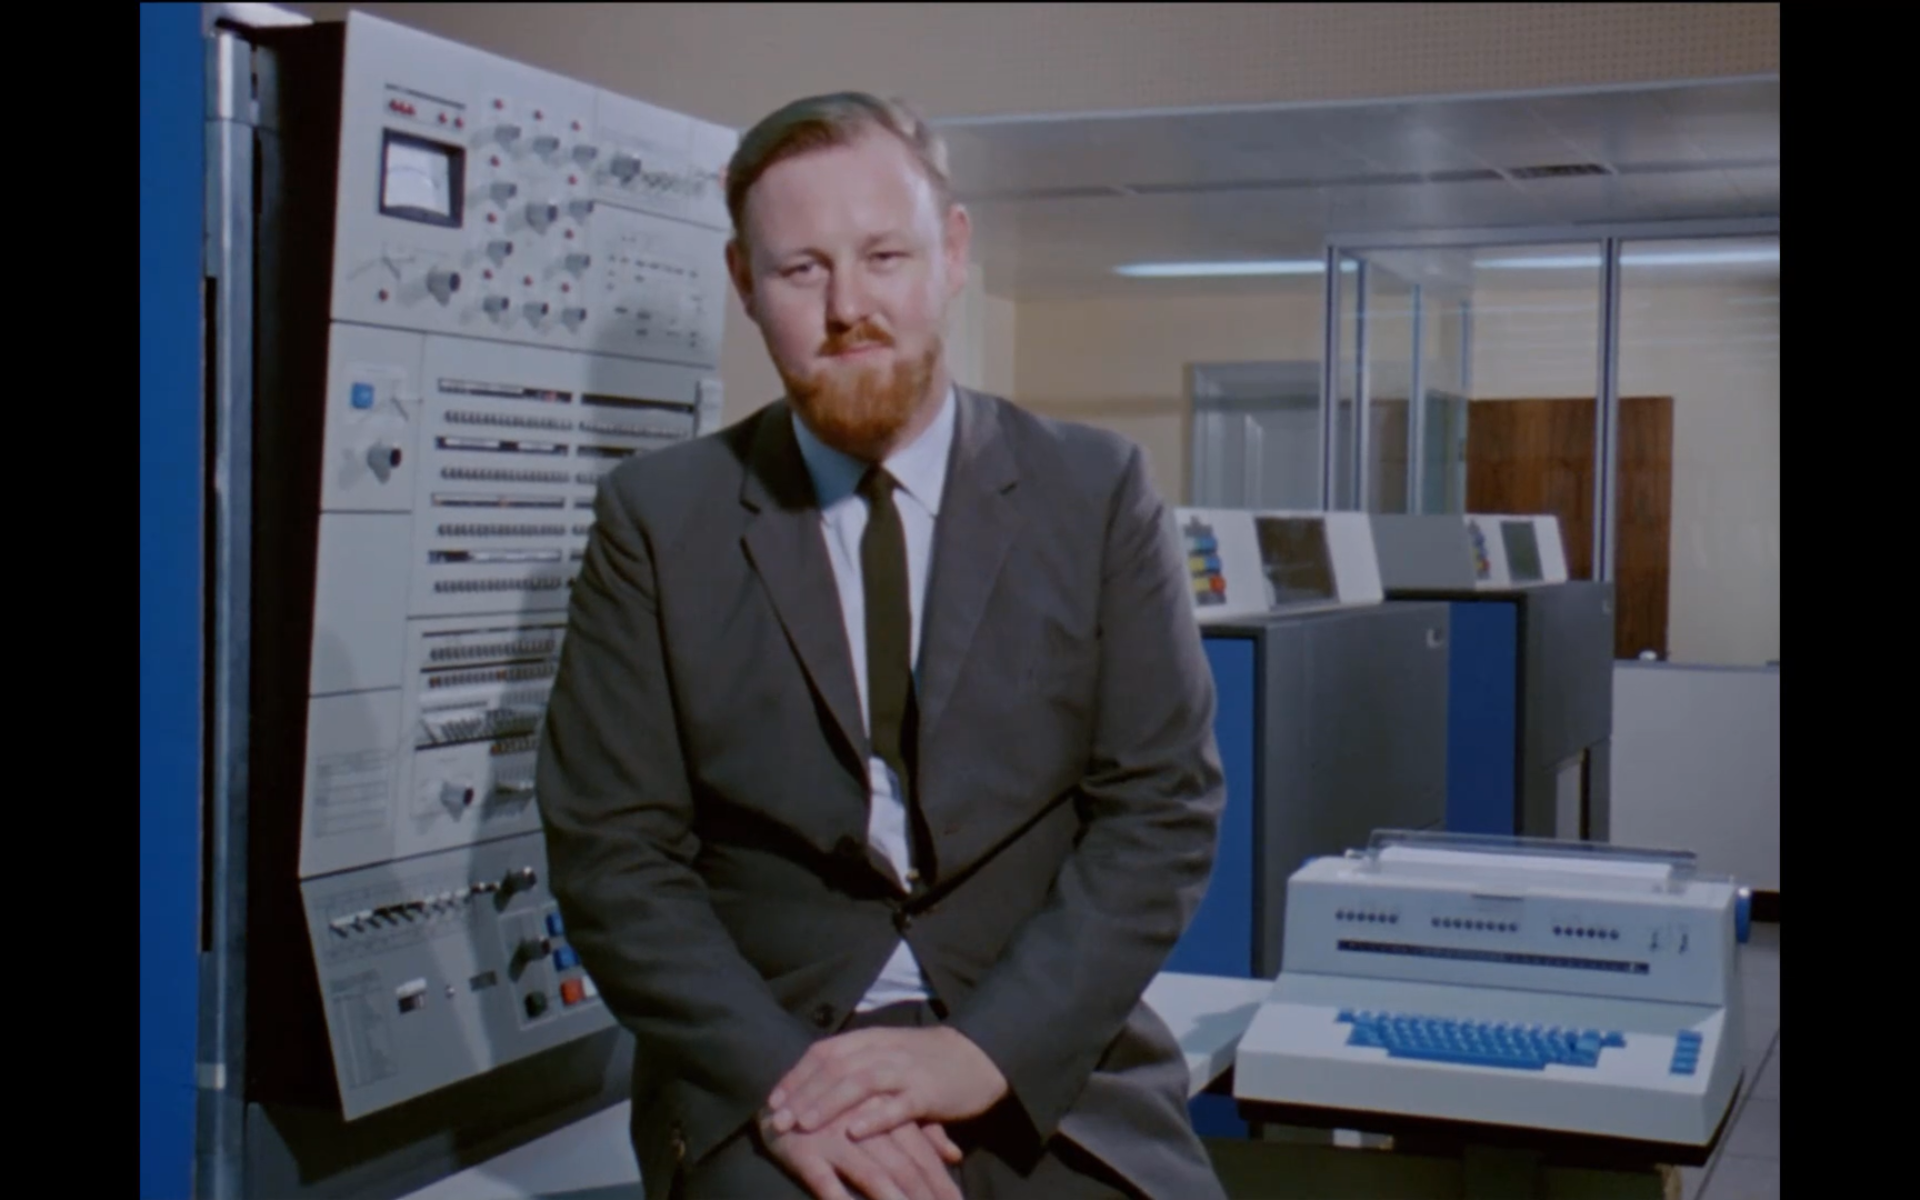
\includegraphics[width=0.75\linewidth]{images/01-data-for-decisions} \caption{Roger Tomlinson talks about the use of computers for the Canada Land Inventory in 1967. Frame from "Data for Decision", a National Film Board of Canada documentary, directed by Michael Millar.}\label{fig:1-data-for-decisions}
\end{figure}

It was 29-year old Roger Tomlinson who recognized the need for computers to handle the massive influx of mapped data (Figure \ref{fig:1-data-for-decisions}). Tomlinson was working in Ottawa for an aerial survey company called Spartan Air Services Ltd., when he serendipitously met the head of the Canada Land Inventory, Lee Pratt, aboard a flight. Pratt and Tomlinson exchanged ideas about creating a computer system for handling mapped data and Tomlinson got to work to lead the development of the world's first computerized GIS. That was 1962. Tomlinson first described it as a ``geo-information system'' \citep{Tomlinson_1967}, but it was later renamed the Canadian Geographic Information System before it was shortened to the \textbf{Canada Geographic Information System (CGIS)}. In the years that followed, the Canada Land Inventory produced over 12,000 map sheets showing the capability of Canada's lands for agriculture, forestry, recreation, and wildlife \citep{fisher_overview_1979}. A major early function of the CGIS was to scan and digitize maps, all of which were on paper sheets. This time is best thought of as ``cartographic puberty'', the awkward but necessary transition from paper to magnetic tape.

The months that followed are best described as cartographic puberty, the awkward but necessary transition from paper to magnetic tape. Thousands of existing paper maps had to be scanned, one line at a time, by a drum scanner. To scan a paper map with these machines required feeding the large paper map into the belly of a cylindrical drum so that as the drum spun a little optical head focused a light onto a small area and a photomultiplier together with a detector recorded the light intensity of the cartographic lines as a digital number. As the drum spins and completes a revolution, the optical head shifts by a fraction of a centimeter to record the next line of the map. In this way, a drum scanner capable of 20,000 samples per second would take about 20 minutes to fully scan a 80 x 60 cm paper map at a resolution of 0.02 cm. Other advances in computer hardware were achieved as a result of the pioneering work by Tomlinson, including the development and integration of digitizer and plotter tables for inputting and updating geographic data into the computer. Tomlinson is widely acknowledged as the creator of modern computerized GIS.

\begin{figure}
\includegraphics[width=0.75\linewidth]{images/01-Canada-land-inventory} \caption{Excerpt from a brochure describing initial mapping efforts of the Canada Land Inventory in British Columbia. Published by the Minister of Supply and Services Canada, n.d.}\label{fig:1-Canada-land-inventory}
\end{figure}

While the Canada Land Inventory was underway with the aid of the CGIS, provinces moved to create the agricultural land reserves to ensure that the most fertile areas remained available as farmland. In 1973, British Columbia established the Agriculture Land Reserves, setting aside 5\% of its land base for farming priority. Newfoundland and Labrador established an Agriculture Development Area around the city of St.~John's in the same year. By 1977, it was learned from CGIS analysis that only 0.5\% the second largest country in the world supports prime farmland and half of that occurs in the vicinity of the most populous metropolitan area: Toronto (Figure \ref{fig:1-cli-agriculture-capability-toronto}) \citep{manning_overview_1977}. Ontario published Food Land Guidelines the next year that effectively laid out a land use planning framework for municipalities and the province to protect and maximize the efficiency of farming on the best available land \citep{ministry_of_agriculture_and_food_food_1978}.

By 1979, the Canada Land Inventory produced over 12,000 map sheets showing the capability of Canada's lands for agriculture, forestry, recreation, and wildlife \citep{fisher_overview_1979}. These maps represented the first digital overlays and analyses of land capability in the world and they covered much of Canada from the Atlantic Ocean to the Pacific Ocean.

\textbackslash begin\{figure\}

\{\centering \includegraphics[width=1\linewidth]{images/01-cli-agriculture-capability-toronto}

\}

\textbackslash caption\{Soil capability for agriculture from the Canada Land Inventory for the area surrounding Toronto, Canada. The majority of the best soils for farming in Canada (Class 1 - No significant limitations in use for crops) are found in southeastern Ontario. \textless a
\textbackslash href=`\url{https://www.opengeomatics.ca//\#fig:1-cli-agriculture-capability-toronto}'\textgreater Interactive web map can be viewed in the web browser version of the textbook. Queen's Printer, Public Domain.\}\label{fig:1-cli-agriculture-capability-toronto}
\textbackslash end\{figure\}

\section{Environmental Management Imperatives}\label{environmental-management-imperatives}

On the opposite shore of Lake Erie from where some of the best Canadian soils for farming were deposited millennia ago by the glacial processes that formed the Great Lakes, the Cuyahoga River quietly empties a small drainage basin of approximately 2,100 km\textsuperscript{2} and bisects the city of Cleveland, Ohio in the United States. This relatively small, crooked river is one of many that fills Lake Erie and flows slowly by former sleepy industrial towns along the lake shore. The first European settler built his cabin on the shore of the Cuyahoga River in 1797 at the site of present-day Cleveland and over the next 155 years of industrialization, the river was reported to have caught fire nine times \citep{la_bella_not_2009}. Ignited once every 17 years or so from volatile oil slicks and other pollutants suspended in the water column (Figure \ref{fig:1-Cuyahoga-River-fire-1952}).

\begin{figure}
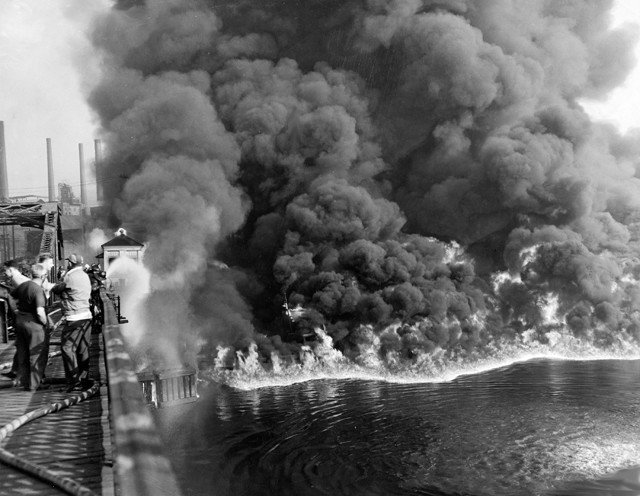
\includegraphics[width=0.75\linewidth]{images/01-Cuyahoga-River-fire-1952} \caption{The Cuyahoga River burns in 1952 near Cleveland, Ohio in the United States as an oil slick is ignited. Special Collections, Cleveland State University Library.}\label{fig:1-Cuyahoga-River-fire-1952}
\end{figure}

In 1968, 16 years after the last burning, just 60 km upstream, a symposium at Kent State University described the state of a 4 km reach of the river \citep{kent_state_university_cuyahoga_1968}:

\begin{quote}
{[}\ldots{]} Large quantities of black heavy oil floating in slicks, sometimes several inches thick, are observed frequently. Debris and trash are commonly caught up in these slicks forming an unsightly floating mess. Anaerobic action is common as the dissolved oxygen is seldom above a fraction of a part per million. The discharge of cooling water increases the temperature by 10 to 15 °F {[}5.6 to 8.3 °C{]}. The velocity is negligible, and sludge accumulates on the bottom. Animal life does not exist.
\end{quote}

The following year in the summer of 1969, the Cuyahoga River burned again. This time, the fire ignited a national conversation in the United States about pollution and was a catalyst for the passage of landmark legislation for protecting the environment. A month after the fire was extinguished, the United States Senate unanimously passed the National Environmental Policy Act (NEPA), legislation that required the federal government to consider the environmental impact of its land use. The following year, the Environmental Protection Agency was established by an executive order of President Nixon and the Clean Air Act was passed. By 1972, the United States Congress passed the Clean Water Act. These events in the late 1960s and early 1970s provided new environmental and regulatory imperatives for the continued development of computerized GIS.

By 1976, the United States Fish and Wildlife Service solicited bids to build a GIS for evaluating the impacts of coal strip mining on wildlife habitat. Part of the initial work involved scoping out the operational capabilities of nearly all available GIS applications that were available at the time \citep{usfws_1977}. When the GIS was completed in 1978, it was named the Map Overlay and Statistical Software (MOSS). An important advancement with MOSS was the ability to handle both raster and vector data. Prior GIS software handled one or the other and there was a growing need to integrate both as vector maps were being overlaid with newly available satellite imagery.

The first earth-observing Landsat satellite was launched in 1972. Since then, eight more Landsat satellites have been launched and the program represents the longest-running historical record of Earth's changing surface. Images from the first Landsat satellite actually resulted in the discovery of a new island off the northeast coast of Labrador, aptly named Landsat Island. The discovery of Landsat Island was as Canadian as its ground verification, which was performed by Dr.~Frank Hall of the Canadian Hydrographic Service in 1976 and later recounted by Member of Parliament Scott Reid \citep{reid_parliamentary_2001}:

\begin{quote}
I have spoken to Frank Hall Sr.~and he told me a fascinating story about the moment of discovery. He was strapped into a harness and lowered from a helicopter down to the island. This was quite a frozen island and it was completely covered with ice. As he was lowered out of the helicopter a polar bear took a swat at him. The bear was on the highest point on the island and it was hard for him to see because it was white. Hall yanked at the cable and got himself hauled up. He said he very nearly became the first person to end his life on Landsat Island.
\end{quote}

In 1980, the United States Army Construction Engineering Research Laboratory began work on a new GIS that would come to be known as the Fort Hood Geographic Information System. This early GIS was a significant investment by the United States military for undertaking environmental assessment and impact of operations at military installations as required by the earlier NEPA legislation. The Fort Hood GIS would later be renamed GRASS (Geographic Resources Analysis Support System) as it became operationalized at other military installations. \href{https://github.com/OSGeo/grass}{GRASS} continues to be one of the most significant GIS software packages today because it was initially released in the public domain and later developed as Free and Open Source Software (FOSS). As a result of this pioneering thought, many software packages have followed suit and there is now a robust community of FOSS development for GIS including another popular package called \href{https://github.com/qgis/QGIS}{QGIS} (Quantum GIS).

\section{Geomatics Today}\label{geomatics-today}

Today, there are a variety of advancements in technology and information that have changed how geomatics allows us to address environmental management issues. A rapid revolution of remote sensing has occurred since the early days of the Landsat program. Today, there are over 150 Earth-observing satellites orbiting above our heads and constantly collecting data about Earth's atmosphere, biosphere, lithosphere, hydrosphere, and cryosphere. The Landsat program alone has generated over 10 million images over the last 40 years. The amount of data produced from all Earth-observing satellites has increased from 1 PB (petabyte or 1,024 terabytes) over the last 15 years to 1 PB produced every single day. The increase in data availability is made possible by miniaturization of computers, processors, and electronic storage as well as near real-time processing of data in the cloud through networks of computers connected by the internet. Today, there are now commercialization and globalization imperatives for GIS. The cooperation of dozens of nations around the world have lead to successful space and Earth-observing programs and now even space itself is commercializing with satellite missions launched by private corporations. In fact, geomatics is now a field extending beyond Earth with significant applications on Mars and our other planetary neighbours.

Demand for and use of geographic information has never been higher in human history. With the advent of mobile phones, we consume and produce geographic data on a daily basis for navigation, working out, gaming, finding new restaurants, and meeting our friends. Many of the original technologies developed with environmental imperatives are today used in some of our favourite mobile applications like Uber, Pokemon Go!, Waze, and Google Maps. The new information age has also presented new challenges and ethical questions related to individual privacy and so-called volunteered geographic information, which is mapped information created by non-professionals.

In the chapters that follow, we will explore in more depth all aspects of the science and technology of this exciting field. As you read through the remaining chapters, see if you can identify the different components of GIS. Perhaps you might recognize the evolution and next generation of some of the early technologies. As you read, reflect on the science of the applications in the detailed case studies. The textbook is yours to explore the field of geomatics with interactive visualizations, reflection questions, and practice questions at the end of each chapter.

\section{Summary}\label{summary}

Geomatics is the science and technology of collecting geographic data and converting it to geographic information for use in a wide variety of industries. A geographic information system (GIS) is comprised of components that interact and interrelate to allow us to undertake powerful spatial analysis, produce maps, and model the world around us. Key technology advancements including the photograph, airplane, and computer have enabled practically all aspects of modern geomatics. Canada was an incubator for these technologies to develop into the first GIS for a practical environmental and land use problem. The historical developments in geomatics have impacted many aspects of our lives today and continues to support decision-making for managing our environment.

\section*{Reflection Questions}\label{reflection-questions}
\addcontentsline{toc}{section}{Reflection Questions}

\begin{enumerate}
\def\labelenumi{\arabic{enumi}.}
\tightlist
\item
  What is the difference between a conceptual model and a spatial model?
\item
  What was the initial motivation for developing the first GIS?
\item
  Give an example of a spatial question that could be answered by a GIS.
\end{enumerate}

\section*{Practice Questions}\label{practice-questions}
\addcontentsline{toc}{section}{Practice Questions}

\begin{enumerate}
\def\labelenumi{\arabic{enumi}.}
\tightlist
\item
  Name the five components of GIS.
\item
  What is a model? Give an example of a model.
\item
  What was the name of the first computerized GIS? Who developed it?
\item
  Which technologies where instrumental in the development of GIS?
\item
  Which early GIS was able to handle both vector and raster data?
\item
  Name two other open source GIS software.
\end{enumerate}

\chapter{Mapping Data}\label{mapping-data}

Written by
Paul Pickell

You probably already accept that the Earth is ``round'' and not ``flat''. You have probably held and touched a globe at some point in your life. But have you ever wondered how we describe location and measure something as large as the Earth? In this chapter, we will explore fundamental concepts for how we measure the Earth and orient ourselves with coordinate systems.

\section*{Learning Objectives}\label{learning-objectives-1}
\addcontentsline{toc}{section}{Learning Objectives}

\begin{enumerate}
\def\labelenumi{\arabic{enumi}.}
\tightlist
\item
  Understand the models of Earth's figure and shape
\item
  Describe different vertical datums and how they are used to reference height
\item
  Understand the difference between cartesian, celestial, geographic, and projected coordinate systems
\item
  Recognize the differences among major types of map projections
\item
  Explore how projected coordinate systems distort and represent the world around us
\end{enumerate}

\section*{Key Terms}\label{key-terms-1}
\addcontentsline{toc}{section}{Key Terms}

Antipode, Great Circle, Small Circle, Geodesy, Vertical Datum, Horizontal Datum, Deflection of the Vertical, Ellipsoid, Spheroid, Geoid, Elevation, Orthometric Height, Geoid Height, Geodetic Height, Coordinate System, Celestial Coordinate System, Cartesian Coordinate System, Geographic Coordinate System, Projected Coordinate System, Map Projection, Tissot's Indicatrix

\section{Introduction to Geodesy}\label{introduction-to-geodesy}

\textbf{Geodesy} is the fascinating science of measuring the shape, orientation, and gravity of Earth. Naturally, some of the questions that come to mind when thinking about such a grand topic are \emph{I thought the shape of Earth is a sphere?} and \emph{How do we orient ourselves on Earth?} and \emph{What does gravity have to do with mapping location?}

All of these questions stem from need to represent \textbf{location}. For our purposes, location is the position of something relative to something else. In order to actually describe a location on Earth, we first need to know the size and shape of Earth. Some of the first estimations of Earth's size and shape were made by Eratosthenes, a Greek mathematician from the second and third centuries B.C. Eratosthenes was responsible for many concepts we use in our everyday lives:

\begin{itemize}
\tightlist
\item
  Conceiving the first spherical model of Earth
\item
  The first accurate measure of Earth's circumference
\item
  Calculating the tilt of Earth's axis
\item
  Calculating the distance of Earth to the Sun
\item
  Invention of the leap day
\end{itemize}

Eratosthenes accurately calculated the circumference of Earth by noticing how the Sun shone directly down the bottom of a well in Syene (modern Egypt) at noon on the summer solstice. He later made a second observation at Alexandria at noon on the summer solstice with a pole and noticed a shadow. He measured the angle of the shadow and inferred the circumference of Earth, which was already known to be spherical (Figure \ref{fig:2-Eratosthenes}).

\begin{figure}
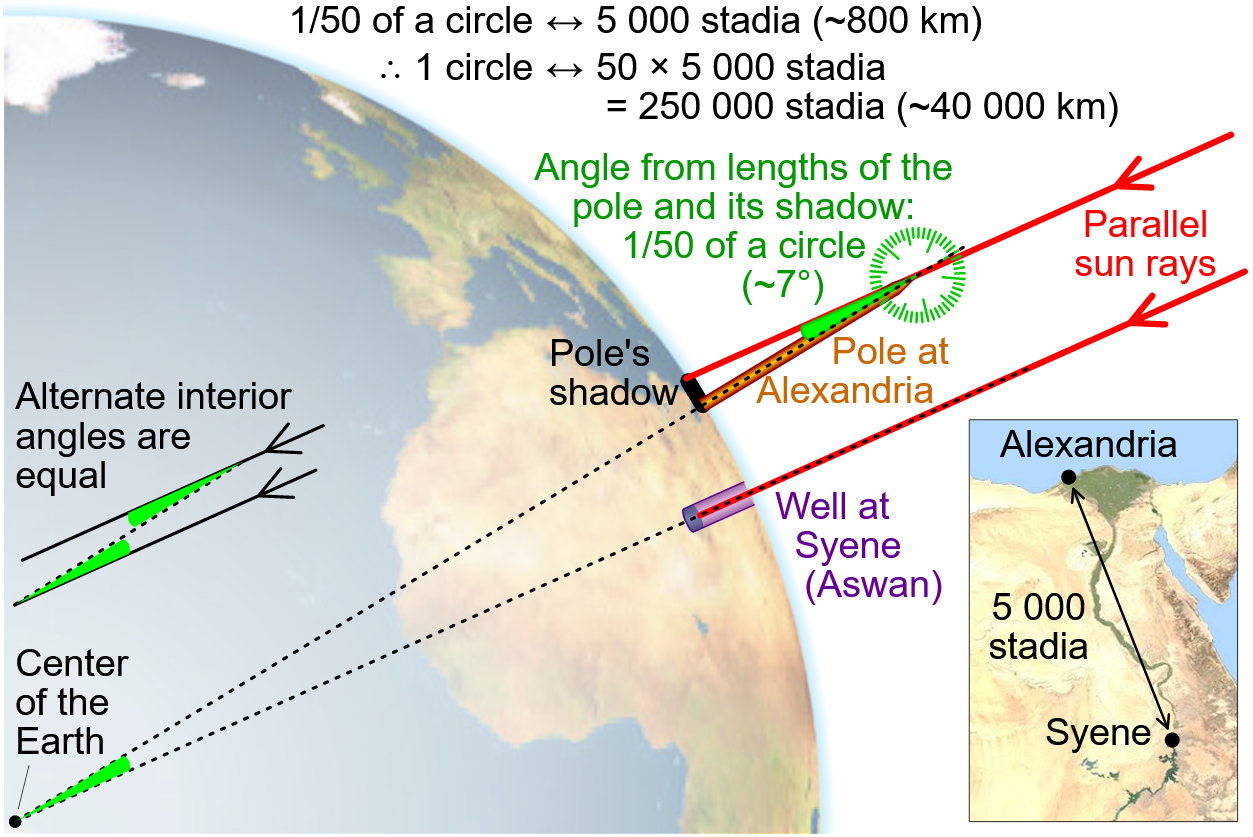
\includegraphics[width=0.75\linewidth]{images/02-Eratosthenes} \caption{Diagram showing how Eratosthenes estimated the circumference of Earth by observing the angle of a shadow that was cast about 800 km north of Syene in present-day Egypt. @monniaux_illustration_2005, CC-BY-SA-4.0.}\label{fig:2-Eratosthenes}
\end{figure}

Pretty simple, right? Turns out, Eratosthenes was off by only 75 km or less than 0.2\% in his calculation! The actual North-South circumference of Earth is about 40,075 km. His calculation worked because the Sun's rays are nearly parallel when they strike Earth. So if you observe the Sun at the same time in two locations on Earth on the North-South axis, you will notice the Sun has a different elevation above the horizon, which means different lengths of shadows will be cast on the ground. This is also a way to prove that the Earth is in fact round because a flat Earth would have equally-sized shadows everywhere at any given time of day.

\section{Models of Earth}\label{models-of-earth}

Here is a simple thought experiment to consider. Suppose you are trying to measure your own height. You probably have not given much thought about how to technically do this because it seems intuitive: place a measuring tape at the bottom of your feet and mark the measurement at the top of your head. If we break this down, there are some important rules to follow (Figure \ref{fig:2-height}):

\begin{enumerate}
\def\labelenumi{\arabic{enumi}.}
\tightlist
\item
  The measuring tape must originate somewhere. In other words, we need to define a reference point or surface of zero height (i.e., the ground).
\item
  The measuring tape must be a straight line and originate at a 90-degree angle, perpendicular to the ground.
\item
  The measurement must terminate at a point along an imaginary line that is tangential to your head, and yes, that line must be perpendicular to the measuring tape and also parallel with the ground.
\end{enumerate}

\begin{figure}
\includegraphics[width=0.75\linewidth]{images/02-height} \caption{Diagram for measuring height above a datum. Pickell, CC-BY-SA-4.0.}\label{fig:2-height}
\end{figure}

Whenever you measure your height, the ground is easy to define. It is whatever point you are standing on. This starting point it also known as a \textbf{datum}. A datum is simply a reference point, set of points, or a surface from which distances can be measured. It does not matter if you are below sea level, atop Mount Everest, or on the 30th floor of a skyscraper. You will always get an accurate and repeatable measure of your height using a datum that is defined directly below your feet. But what about measuring the height of terrain on Earth? Whenever we measure the height of Earth's terrain above some reference surface, we are measuring \textbf{elevation}.

The same rules above apply when we measure elevation. In order for elevation measurements to be comparable across the world, we need to define a reference surface, a datum, for the entire planet. There are actually several ways that we can model the shape of Earth in order to produce a datum. Models of Earth's shape are often referred to as either vertical datums (the plural of datum) if you are referencing elevation or horizontal datums if you are referencing location. A \textbf{vertical datum} is a 3D surface model that is used to reference heights or elevations for the Earth. A simple question like \emph{How high is Mount Logan in Yukon, Canada?} is complicated by the need for a reference surface and the fact that Earth's shape is irregular. In this section, we will review three types of vertical datums:

\begin{itemize}
\tightlist
\item
  Geodetic - based on geometry
\item
  Tidal - based on sea level
\item
  Gravimetric - based on gravity
\end{itemize}

\subsection{Geodetic Vertical Datums}\label{geodetic-vertical-datums}

A \textbf{geodetic vertical datum} is one that describes the Earth's shape in the simplest possible terms using standard geometry. Despite what a globe might lead you to believe, the Earth is not perfectly spherical, but it is close to being spherical. In fact, the radius of Earth varies by no more than 22 km or 0.35\%, hardly anything you would ever notice if you were holding it in your hand. That small difference is, however, significant enough to lead to mapping inaccuracies at the local level if a spherical model of Earth was adopted (Figure \ref{fig:2-geodetic-datum}). Instead, we frequently describe Earth's shape as an oblate ellipsoid, which is essentially a sphere that has been flattened, and we define this ellipsoid with a semimajor and semiminor axis. Sometimes you will see the term \emph{spheroid} used, which just means ``sphere-like'' and is interchangeable with the term \emph{ellipsoid}.

\begin{figure}
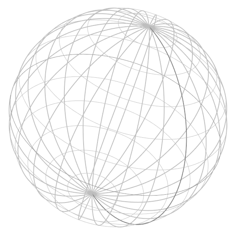
\includegraphics[width=0.5\linewidth]{images/02-geodetic-datum} \caption{Spherical geodetic datum. Pickell, CC-BY-SA-4.0.}\label{fig:2-geodetic-datum}
\end{figure}

There are many different ellipsoids that have been defined and are currently in use as datums. The most commonly used ellipsoid is called the World Geodetic System of 1984 or usually abbreviated as WGS 1984 or WGS 84. In fact, there are hundreds of ellipsoids that have been defined over recent centuries to model the shape of the Earth. The reason for so many other ellipsoids is due in part to technological advances that have improved the accuracy and precision of surveying as well as estimation of the ellipsoidal parameters. Many of these ellipsoids are not \textbf{geocentric}, that is, not originating from the center of mass of Earth. These datums are known as \textbf{regional datums}, which still describe the dimensions that approximate the shape of Earth, but are instead oriented so that the surface of the ellipsoid is congruent with a particular regional surface of Earth. For example, the European Datum 1950, the South American Datum 1969, the North American Datum 1983, and the Australian Geodetic Datum 1966 conform well to their respective continents, even better than WGS 1984 in most cases, but poorly anywhere else in the world.

\begin{figure}
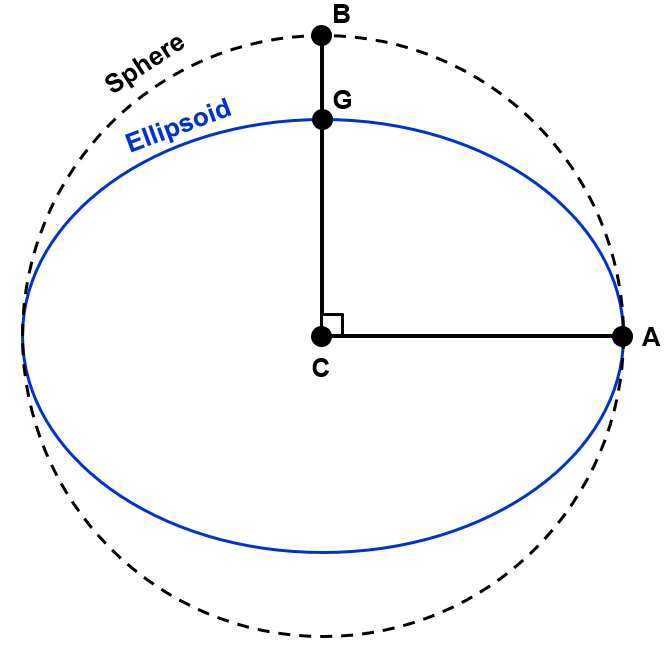
\includegraphics[width=0.75\linewidth]{images/02-sphere-ellipsoid} \caption{Sphere versus ellispoid. Pickell, CC-BY-SA-4.0.}\label{fig:2-sphere-ellipsoid}
\end{figure}

Figure \ref{fig:2-sphere-ellipsoid} greatly exaggerates the flattening of the ellipsoid to illustrate the above points. In reality, the sphere is flattened using a flattening factor calculated as \(f=(CA-CG)/CA\) and defined exactly as \(f=298.257223560\) for WGS 1984. Thus, the semiminor axis (i.e., rotational axis) for the WGS 1984 ellipsoid (meters) is

\[
CG=CA-(CA×\frac{1}{f})=6378137-(6378137×\frac{1}{298.257223560})=6356752.3
\]
where \(G\) is the North Pole and \(A\) is a point on the Equator. The sphere, of course, is much simpler where \(radius=CB=CA=6378137\).

\subsection{Tidal Vertical Datums}\label{tidal-vertical-datums}

A \textbf{tidal vertical datum} is likely one that you are familiar with. The premise of a tidal vertical datum is to use mean sea level as a reference surface, above which are positive elevations and below are negative elevations. This has a lot of advantages, like it is intuitive and oceans cover more than 70\% of the planet's surface so much of Earth's land mass is near an ocean. However, the disadvantages are that sea level changes over time with tides and also with climate change. The not-so-obvious problem with a tidal vertical datum is that the sea level is actually not constant around the planet not only due to tides, but also temperature, air pressure, and gravity. In other words, mean sea level measured at a gauge station in Halifax on the Atlantic Ocean will not be the same distance from the center of Earth as mean sea level measured at Victoria on the Pacific Ocean (Figure \ref{fig:2-tidal-datum}). The primary challenge with a tidal vertical datum is extending it away from the coastline through a network of survey points using a process known as levelling, and even still, it is only meaningful during the epoch in which the mean sea level was measured at a number of tidal gauge stations.

\begin{figure}
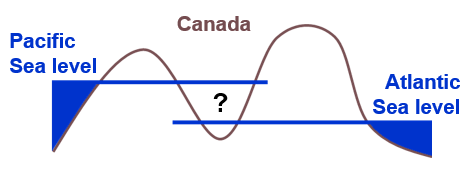
\includegraphics[width=0.75\linewidth]{images/02-tidal-datum} \caption{Conceptual tidal datum for Canada. Pickell, CC-BY-SA-4.0.}\label{fig:2-tidal-datum}
\end{figure}

\subsection{Gravimetric Vertical Datums}\label{gravimetric-vertical-datums}

The \textbf{geoid} is a physical approximation of the figure of Earth. The shape represents Earth's surface with calmed oceans in the absence of other influences such as winds and tides. It is computed using gravity measurements of Earth's surface and is best thought of as the surface or shape that the oceans would take under the influence of Earth's gravity and rotation alone. In other words, the geoid represents the shape Earth would take if the oceans covered the entire planet. More specifically, the geoid is a \textbf{gravimetric} model of Earth's shape that is defined as an equipotential surface from a constant gravity potential value. Due to the distribution of mass on Earth, gravity is not constant across the planet's surface. As a result, the surface of Earth's oceans is not smooth like a sphere, but instead undulates depending on where gravity forces water to remain at rest. You can think of Earth's gravitational field as a series of parallel lines extending outwards from the center of mass of Earth into space. Any of these lines that you choose is an equipotential surface where the force of gravity is constant. Keep in mind that the force of gravity is stronger nearer the center of mass of Earth and weaker as you move away from it. Thus, the geoid is an arbitrary equipotential gravity surface that is chosen to roughly coincide with present-day mean sea level.

When you measure the height of something relative to a gravimetric vertical datum like the geoid, you must level your instrument. Levelling forms a vertical line that is orthogonal or perpendicular to the geoid, known as a \textbf{plumb line}. It is incredibly easy to visualize a plumb line. Simply tie a rock to the end of a string and hold the string with your outstretched arm. The length of the straightened string traces a plumb line to the center of mass of Earth, wherever you are. Because gravity changes with location on Earth and all plumb lines are converging on a singular point, plumb lines are never parallel. This phenomenon has important implications for comparing observations on the the ground with a geodetic model of Earth like an ellipsoid. In other words, the plumb line that you traced with your string is pointing to the center of mass of the geoid, but the center of the ellipsoid is often in a slightly different direction. This difference is known as the \textbf{deflection of the vertical} and is measured as the angular difference between the centre of the geoid and the centre of a reference ellipsoid. Like other measurements of geodetic location (i.e., latitude and longitude), the deflection of the vertical is comprised of two angles: \(ξ\) (xi) representing the north-south angular difference and \(η\) (eta) representing the east-west angular difference.

It should be evident by now that the reference surface that you choose as a vertical datum will determine the measured elevation of Earth's terrain. Additionally, We frequently need to convert elevations between geodetic and gravimetric vertical datums. For example, when you use a Global Navigation Satellite System receiver, you are provided with an elevation that is relative to the WGS 1984 ellipsoid. The difference in height between an ellipsoid and the geoid is referred to as \textbf{geoid height (N)} while the difference in height between an ellipsoid and Earth's surface is referred to as \textbf{geodetic or ellipsoidal height (h)}. The difference in height between the geoid and the Earth's surface is called \textbf{orthometric height (H)} (Figure \ref{fig:2-H-h-N}), and is given as:

\[
H = h - N
\]

\begin{figure}
\includegraphics[width=0.75\linewidth]{images/02-H-h-N} \caption{Orthometric Height (H) is the ellipsoidal height (h) less the geoid height (N). Pickell, CC-BY-SA-4.0.}\label{fig:2-H-h-N}
\end{figure}

To illustrate the concept of a gravimetric datum, suppose we constructed a large, straight tunnel through the physical Earth that was tangential to the ellipsoid. If we allowed the oceans to flow freely through this tunnel, your experiences might convince you that water would flow from one end to the other. But in fact, this tunnel is so large, that the gravity field is changing. So the water would actually come to rest at the surface of the geoid or gravimetric model, as shown in Figure \ref{fig:2-geoid-tunnel} below.

\begin{figure}
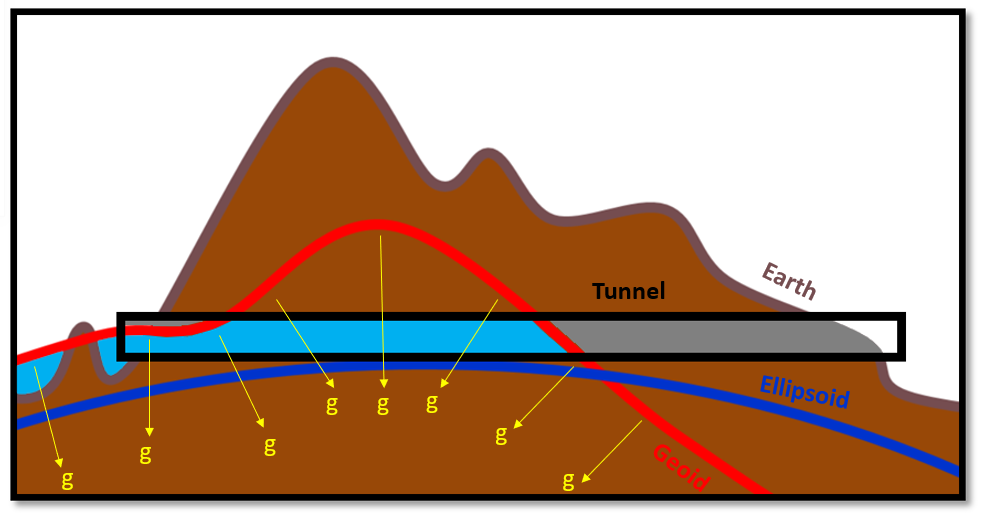
\includegraphics[width=0.75\linewidth]{images/02-geoid-tunnel} \caption{Thought experiment showing where water would be at rest within a tunnel through the geoid due to the equipotential force of gravity (g). Pickell, CC-BY-SA-4.0.}\label{fig:2-geoid-tunnel}
\end{figure}

\section{Case Study: The Canadian Geodetic Vertical Datum of 2013}\label{case-study-the-canadian-geodetic-vertical-datum-of-2013}

The Canadian Geodetic Vertical Datum of 2013 (CGVD2013) is the current gravimetric vertical datum used in Canada to reference heights. It is defined with a potential gravity value of 62,636,856.0 \(m^2\) \(s^-2\). The pervious vertical datum in Canada - the Canadian Geodetic Vertical Datum of 1928 (CGVD28) - was actually a tidal vertical datum that corresponded to mean sea level measured at Yarmouth, Halifax, Pointe-au-Père, Vancouver and Prince-Rupert, and a height in Rouses Point in New York. It turns out that Halifax referenced to CGVD2013 is 64 centimeters \emph{below} Halifax referenced to CGVD28!

For reference, CGVD2013 is 17 centimeters below mean sea level measured in Vancouver at the Pacific Ocean, 39 centimeters above mean sea level in Halifax at the Atlantic Ocean, and 36 centimeters above mean sea level in Tuktoyaktuk at the Arctic Ocean. The older CGDV28 did not have any survey benchmarks in the far north of Canada and, with the advent of more reliable satellite-based measurements, was modernized in 2015 to CGVD2013. The United States currently uses the North American Vertical Datum of 1988 (NAVD88), which was never adopted by Canada, but the United States will be modernizing their vertical datum by adopting a gravimetric model with the same gravity potential value as Canada as early as 2025.

\begin{figure}
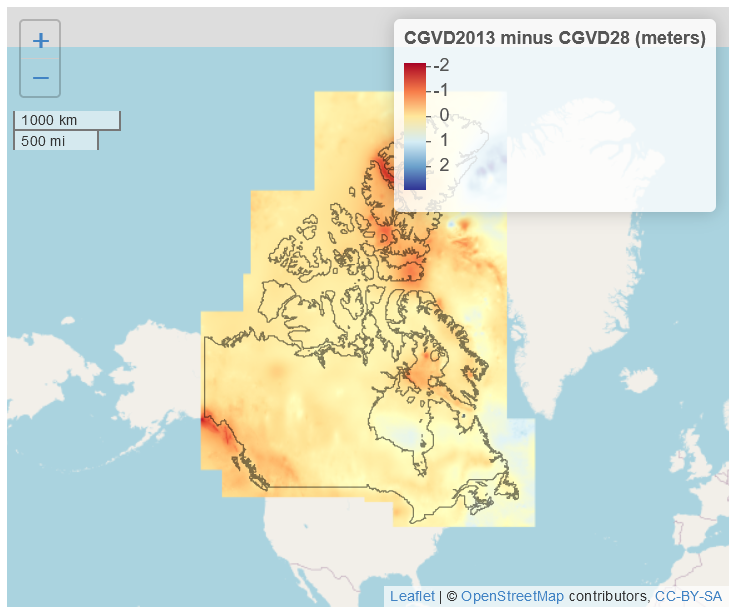
\includegraphics[width=1\linewidth]{images/02-CGVD-leaflet} \caption{The difference (in meters) between the Canadian Geodetic Vertical Datum of 2013 (CGVD2013) and the Canadian Geodetic Vertical Datum of 1928 (CGVD28). <a
  href='https://ubc-geomatics-textbook.github.io/geomatics-textbook/#fig:2-CGVD-leaflet'>Animated figure can be viewed in the web browser version of the textbook</a>. Data from Natural Resources Canada and licensed under the <a href='https://open.canada.ca/en/open-government-licence-canada'>Open Government Licence - Canada</a>. Pickell, CC-BY-SA-4.0.}\label{fig:2-CGVD-leaflet}
\end{figure}

\section{Referencing Location}\label{referencing-location}

\subsection{Cartesian Coordinate Systems}\label{cartesian-coordinate-systems}

Now that we have explored how to reference heights to vertical datums, we will now turn to considering how to reference location on Earth. Before we we jump to the three dimensional case of Earth, consider how you would map your room and identify your location within that room. Assuming you are in a rectangular room, you could easily pick a corner and first measure the distances between the four corners of the room, giving you the dimensions. You could then proceed to measure your distance to any two walls and quite easily define your position within the room relative to the first corner that you picked. This is an example of a \textbf{coordinate system} that provides reference for the relative locations of anything contained within the extent of the coordinate system (i.e., the four corners of your room).

Fundamentally, a coordinate system is defined by a common unit of measurement (e.g., meters, feet, degrees), an orientation defining the direction that measurements positive or negative, and an \textbf{origin}, which is an arbitrary point where the measurements begin at zero. On a one dimensional line, you can define any other location on the line as a measured distance from the origin at \([0]\). On two dimensional maps, like your room, we have two axes that are perpendicular from which we can define any location with measured distances from the origin \([0,0]\). We can also extend this to the three dimensional Earth, which simply requires another axis to define the origin at \([0,0,0]\). All of these cases are referred to as \textbf{Cartesian coordinate systems}, so-named after French philosopher Descartes (also known for the phrase, ``I think, therefore I am'') who first described the two dimensional case in 1637 in \emph{La Géometrie}.

\subsection{Celestial Coordinate Systems}\label{celestial-coordinate-systems}

You might be wondering, \emph{How do we reference locations on Earth?} Before the technological era of geoids, astronomical observations provided the basis for the earliest coordinate systems. The ancient civilizations of Greece, Egypt, and Babylon all recognized the use of celestial coordinate systems for defining the location of stars, planets, and other celestial bodies in the sky. Recall that Eratosthenes, a Greek mathematician living about 2300 years ago, had already worked out the spherical shape of Earth. A celestial coordinate system simply extends the spherical shape of the Earth outward into space to locate objects using angular measurements. It is a \emph{geocentric} coordinate system, that is based on an origin at the center of Earth with an orientation following the rotational axis of Earth (i.e., spinning around the semiminor, North-South axis). This is also known as an equatorial coordinate system, because it is oriented relative to the Equator of Earth. The equatorial coordinate system is the reason why you can navigate by Polaris, the North Star, which would appear nearly directly overhead if you were standing at the North Pole. Even though Earth is not perfectly spherical, astronomical observations have been reliably used for millennia to transit the irregular oceans and terrain of Earth.

\subsection{Geographic Coordinate Systems}\label{geographic-coordinate-systems}

Geocentric coordinate systems are essential for global navigation and mapping. In the modern era, we use \textbf{geographic coordinate systems} (sometimes abbreviated GCS) that are oriented to the rotational axis of Earth, much like the equatorial coordinate system. The origin of a geographic coordinate system is the center of Earth and the units of measurement are degrees of \textbf{longitude} and degrees of \textbf{latitude}. Degrees of latitude (denoted by lambda, \(λ\)) measure the angle from the equitorial plane North (+) or South (-), while degrees of longitude (denoted by phi, \(φ\)) measure the angle from the polar plane East (+) or West (-). Thus, geographic coordinate systems use angular units of measurement. Any combination of latitude and longitude gives coordinates \([λ,φ]\) on a sphere or ellipsoid. Positive values of latitude put you in the Northern Hemisphere, while negative values of longitude put you in the Western Hemisphere. Constant lines of latitude, known as \textbf{parallels} because they are always parallel to one another, and lines of longitude, known as \textbf{meridians}, form a grid that fits over a sphere or ellipsoid called a \textbf{graticule}.

For most of your life, you have probably believed that there is a singular combination of capital-L Latitude and Longitude values that absolutely define some location on Earth in perpetuity. This is perhaps the most profound geographic lie that we were taught as young school children. In fact, there are as many ``types'' of latitude as there are geographic coordinate systems. By now, you should be able to recognize the difference between \emph{geocentric latitude} that is referenced to a sphere and \emph{geodetic latitude} that is referenced to an ellipsoid. The main difference is that geocentric latitude is the angle relative to the centre of the sphere at the equatorial plane and geodetic latitude is the angle relative to the equatorial plane (i.e., not necessarily the centre). Figure \ref{fig:2-geocentric-geodetic-latitude} illustrates how the same angle can put you in two very different places depending on the geographic coordinate system you are using.

\begin{figure}
\includegraphics[width=0.75\linewidth]{images/02-geocentric-geodetic-latitude} \caption{Geocentric versus geodetic latitude. Pickell, CC-BY-SA-4.0.}\label{fig:2-geocentric-geodetic-latitude}
\end{figure}

\(CS\) represents the line connecting the centre of a spherical geographic coordinate system to the surface of the sphere at a geocentric latitude \(φ′=45°\) and \(DE\) represents the line connecting the equatorial plane to the surface of the ellipsoid at a geodetic latitude \(φ=45°\). Notably, \(CS\) is parallel to \(DE\) and \(CS\) intersects with the surface of the sphere at a 90° angle and \(DE\) intersects the surface of the ellipsoid at a 90° angle.

A coordinate system that is referenced to an ellipsoid is known as a \textbf{horizontal datum}. For example, the World Geodetic System of 1984 (WGS 1984) is a \emph{geodetic} datum that has a geographic coordinate system referenced to it. So the origin of WGS 1984 is also the origin of the GCS from which latitude and longitude measurements are derived. So if you measured your latitude and longitude using the WGS 1984 horizontal datum, you would be placed somewhere on the ellipsoid also defined by WGS 1984. It is important to note, however, that the same exact \emph{geocentric latitude} and longitude measures would place you somewhere else on a sphere. Other factors such as plate tectonics, glaciation, and ocean tides cause the Earth's surface to be in constant motion underneath any fixed horizontal datum. For example, Europe has drifted about 60 meters from North America since Eratosthenes first calculated the circumference of Earth. Therefore, any ``type'' of latitude or longitude is only useful during a particular epoch of time.

If you mapped the Earth as an ellipsoid in a three dimensional Cartesian coordinate system, you could describe location using three coordinates \([x,y,z]\), with \([0,0,0]\) being the center of Earth. However, we do not often express mapped coordinates of Earth using Cartesian coordinates. Instead of referring to the North Pole at \([0,0,6356752.3]\) meters (the polar radius of Earth) we usually refer to it with a single coordinate, 90° N. Why? The North and South Poles are the only points on Earth that can be defined with a single coordinate because they coincide with the orientation of a geographic coordinate system. Imagine placing a protractor at a 90° angle relative to a table. If you rotate it along that perpendicular axis, one arm of the protector would spin in a 360° circle, but the other arm of the protractor would always point up or down at 90° in the same direction. For all other locations on Earth, a pair of \([λ,φ]\) coordinates are needed to define location. With space-based global navigation systems it is more common to combine coordinates in both horizontal and vertical datums together. For example, \([λ,φ]\) expresses your location relative to the horizontal datum while \([λ,φ,h]\) expresses your ellipsoidal height (h) at a location and \([λ,φ,H]\) expresses your orthometric height (H) at a location.

\subsection*{Your Turn!}\label{your-turn}
\addcontentsline{toc}{subsection}{Your Turn!}

Use our geodesy tool to visualize the differences between the sphere, ellipsoid, and geoid. You can modify the transparency of the sphere and ellipsoid to see how these geometries vary. Change the flattening of the ellipsoid to achieve different models of Earth. Search for locations with latitude and longitude values and calculate the geoid height. Compare geocentric and geodetic latitudes. The sphere and the ellipsoid models in the visualization represent Earth's equatorial diameter (semi-major axis) as 6,356,752.3 m (i.e., equivalent to WGS 1984) and the geoid elevations are exaggerated by a factor of 0.549 to enhance their appearance.

\begin{figure}
\includegraphics[width=0.75\linewidth]{images/02-geodesy-visualization-static} \caption{Online geodesy tool for visualizing the differences between the sphere, ellipsoid, and geoid. <a href='https://ubcemergingmedialab.github.io/geomatics-textbook/viz/geodesy-viz/'>Click here to access the interactive tool.</a> Floria Gu, CC-BY-SA-4.0.}\label{fig:2-geodesy-visualization-static}
\end{figure}

\subsection{Projected Coordinate Systems}\label{projected-coordinate-systems}

Despite everything covered so far in this chapter, we very rarely see or display geographic data in 3-dimensions. In fact, most geographic data you will likely encounter will be either 1- or 2-dimensional. Geographic coordinate systems are incredibly important for understanding how geographic data are fundamentally ``attached'' to the Earth. However, geographic coordinate systems are not suitable for creating maps, those 2-dimensional spatial models that can be easily displayed on your computer screen or printed on a sheet of paper. Instead, cartographers rely on \textbf{projected coordinate systems} that flatten a 3-dimensional geographic coordinate system to a 2-dimensional map. Really, these projected coordinate systems involve transformations called \textbf{map projections} that convert 3-dimensional coordinate space into 2-dimensional coordinate space, which means the map units are linear such as meters. Whenever we move from a geographic to a projected coordinate system, we lose information, and distortion results.

Cartographers have wrestled with how to project Earth onto a printed page for millennia. The fundamental mathematics for map projections were first comprehensively described by Claudius Ptolemy around 150 C.E. Ptolemy's work \emph{Geography} was one of the earliest treatises on cartography and map making that included an atlas of regional maps of Europe, Africa, and Asia. Ptolemy's work built on and came several centuries following Eratosthenes and earlier Greek geocentric observations by Plato and Aristotle. Ptolemy observed that a globe was the best way to represent the intervals and proportions of Earth's surface without distortion. However, globes are not very useful for looking at regions in detail and you can only see part of a globe at any given time. Thus, a mathematical language is needed to translate a geographic coordinate system to a planar or projected coordinate system. \emph{Geography} was lost to antiquity before it was rediscovered, copied, and translated centuries later, first by Muslim cartographers in the 9th century C.E. and later by Italian cartographers in the 15th century C.E. during the Renaissance, which gave rise to the many types of map projections that we see today.

Because all map projections result in distortion from the loss of the third spatial dimension, it is useful to think about map projections in terms of what they preserve. There are four main characteristics that can be distorted or preserved, which give rise to the primary types of map projections that are in use for environmental management applications:

\begin{itemize}
\tightlist
\item
  \textbf{Conformal} projections preserve shape and angles
\item
  \textbf{Equal-area or equivalent} projections preserve area
\item
  \textbf{Azimuthal} projections preserve direction
\item
  \textbf{Equidistant} projections preserve scale and distances
\end{itemize}

Some map projections can preserve several of these characteristics at once, but only a globe can simultaneously preserve area, direction, distance, and shape. Any map projection will have inherent trade-offs representing these characteristics accurately. It is beyond the scope of this textbook to discuss all map projections. Instead, we will focus on several key examples of map projections that are commonly used for environmental management applications. For a more comprehensive discussion of map projections generally, the reader is referred to \emph{Map Projections: A Working Manual} by \citep{snyder_map_1987}. In the next section, we look at how map projection distortation can be measured.

\subsection{Measuring Map Projection Distortion}\label{measuring-map-projection-distortion}

\textbf{Tissot's Indicatrix} is often used to visualize distortion from map projections, named after Nicholas Auguste Tissot. The metric is relatively simple: Tissot's Indicatrix is a perfect circle on the surface of a 3-dimensional globe, but will form an ellipse whenever projected to a 2-dimensional coordinate system. For this reason, Tissot's Indicatrix is sometimes referred to as Tissot's Ellipse. Since ellipses can vary along two axes, Tissot's Indicatrix can represent areal, angular, and linear map distortions both longitudinally and latitudinally at any location in the map. This is very handy, because we can place Tissot's Indiciatrices (the plural of indicatrix) at different locations and examine how distortion changes throughout the map projection.

So how do we use this tool? The quotient between a line projected onto a map \(a\) and the same line on a globe \(a'\) is \(\frac{a}{a'}=1\) when there is no distortion on that axis of the ellipse. This quotient is also called a scale factor because it is showing how the map scale is modified locally by a map projection. Figure \ref{fig:2-reference-indicatrix} below shows an example of a reference indicatrix that is a perfect circle on a globe with axes \(a\) and \(b\).

\begin{figure}
\includegraphics[width=0.75\linewidth]{images/02-reference-indicatrix} \caption{Reference Tissot Indicatrix. Pickell, CC-BY-SA-4.0.}\label{fig:2-reference-indicatrix}
\end{figure}

Let us assume that \(a = b = 1\). Then, the reference indicatrix has the following properties: \(a=b\), \(a×b=1\), and \(Area=πab=π\). If \(\frac{a'}{a'}>1\), then we can conclude that the the projection is \emph{expanding} the distance along the \(a\) line. If \(\frac{a'}{a'}<1\), then we can conclude that the projection is \emph{compressing} the distance along the line \(a\). For example, suppose \(a=2\) and \(b=0.5\), then we have modified the scale of the indicatrix along both axes, but the areal solution is the same as the reference indicatrix shown as the red dashed circle in Figure \ref{fig:2-reference-equivalent} below.

\begin{figure}
\includegraphics[width=0.75\linewidth]{images/02-equivalent-indicatrix} \caption{Equivalent Tissot Indicatrix. Pickell, CC-BY-SA-4.0.}\label{fig:2-reference-equivalent}
\end{figure}

The indicatrix above in Figure \ref{fig:2-reference-equivalent} is an example of an \emph{equivalent} indicatrix, which has the following properties: \(a>b\), \(a×b=1\), and \(Area=πab=π\).

If \(\frac{a}{a'}×\frac{b}{b'}>1\), then we can conclude that the projection is \emph{inflating} the area. If \(\frac{a}{a'}×\frac{b}{b'}<1\), then we can conclude that the projection is \emph{deflating} the area. Consequently, whenever the quotients of both axes are equivalent (i.e., \(\frac{a}{a'}=\frac{b}{b'}\)), Tissot's Indicatrix forms a perfect circle and the ellipse is conformal with angles true to the globe. For example, suppose \(a=b=2\), then we have modified the scale of the indicatrix along both axes, but with the same factor. This results in a \emph{conformal} indicatrix that is not equivalent, shown in Figure \ref{fig:2-conformal-indicatrix} below.

\begin{figure}
\includegraphics[width=0.75\linewidth]{images/02-conformal-indicatrix} \caption{Conformal Tissot Indicatrix. Pickell, CC-BY-SA-4.0.}\label{fig:2-conformal-indicatrix}
\end{figure}

This conformal indicatrix has the following properties: \(a=b\), but \(a×b≠1\), and therefore \(Area=πab=4π\). As you can see, whenever \(a×b=1\) the indicatrix is equivalent (equal-area) and whenever \(a=b\) the indicatrix is conformal.

\section{Map Projections for Environmental Management}\label{map-projections-for-environmental-management}

\subsection{Mercator}\label{mercator}

Mercator is a cylindrical map projection that represents meridians and parallels as straight lines. The cylindrical surface is oriented such that the rotational axis of Earth runs through the openings of the cylinder and the Equator represents the tangent where the cylinder meets the Earth's surface. Scale along the tangent is true because the translation from the spherical Earth to the cylindrical surface is one-to-one at the tangent, so this is also the location on the projection where there is no distortion. This has the effect of accurately representing the shape and angles on the map (i.e., conformal), but greatly distorts area as you move away from the Equator. In fact, the North and South Poles are represented as 2-dimensional lines at the top and bottom edges of the map instead of 1-dimensional points. Although scale and area change as you move North or South along a meridian, scale and area are equivalent along any parallel, but not necessarily true to a globe. In other words, you can compare area or scale anywhere along a parallel, but only at the Equator is the area and scale true to the globe.

The Mercator map projection is perhaps the most pervasive and reproduced projection around us (Figure \ref{fig:2-Mercator-map}). Because angles are preserved, you can easily and accurately navigate long distances across Earth, and this was exactly the purpose that Gerardus Mercator envisioned when he first identified the projection for sea-faring Europeans in 1569. You may also recognize the Mercator projection from web mapping applications like Google Maps, which use it because it ensures that North-South roads intersect at right angles with East-West roads.

\begin{figure}
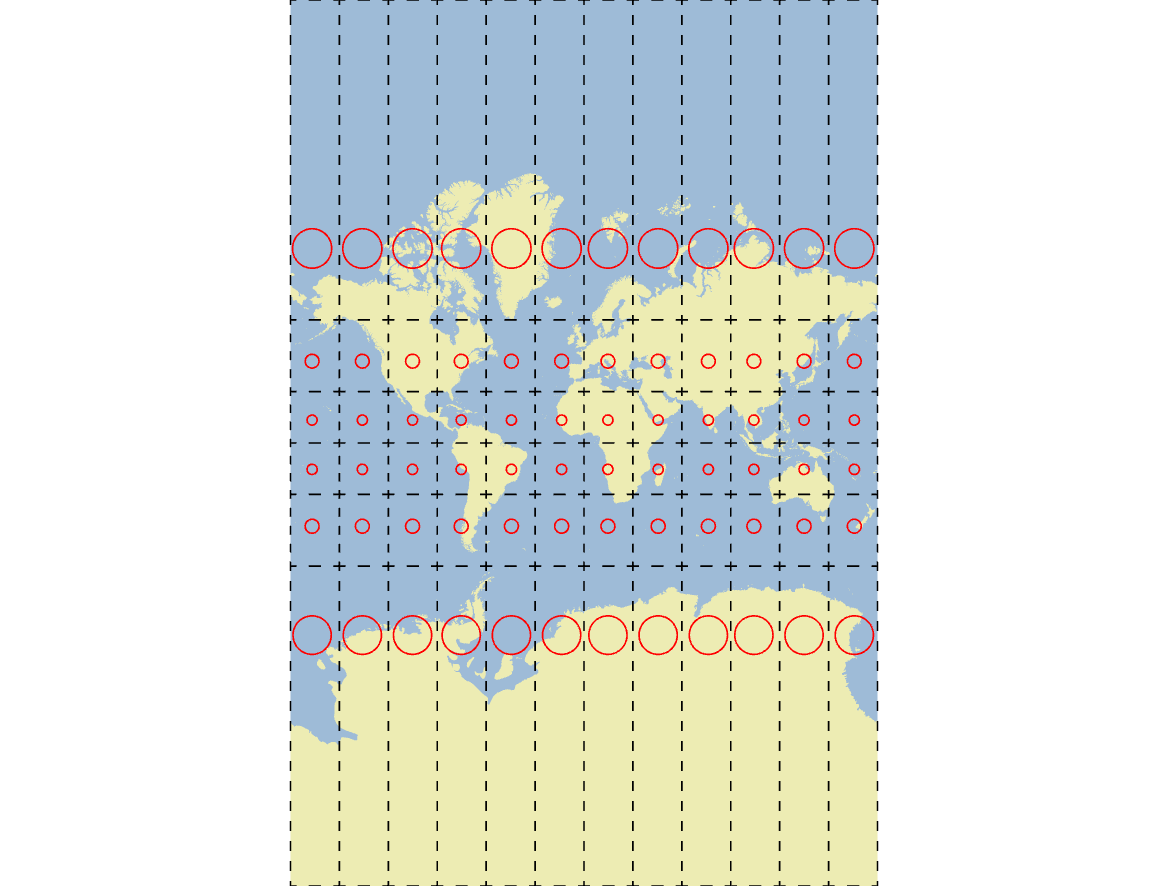
\includegraphics[width=0.75\linewidth]{images/02-Mercator-map} \caption{Mercator map projection with Tissot's Indicatrices in red. Pickell, CC-BY-SA-4.0.}\label{fig:2-Mercator-map}
\end{figure}

\subsection{Universal Transverse Mercator (UTM)}\label{universal-transverse-mercator-utm}

Universal Transverse Mercator (UTM) is very similar to a Mercator projection except that the cylinder is rotated or transverse by 90° so that the opening of the cylinder is perpendicular to the rotational axis of Earth. This has the effect of moving the tangent from the Equator to any Meridian. In fact, you can rotate the cylinder at any angle you want where 0° is a true Mercator, 90° is a transverse Mercator, and any other angle is considered an oblique Mercator. UTM is actually a system of 60 different transverse Mercator projections that are defined to represent 6° Longitudinal intervals of Earth's surface (60 zones x 6° = 360°). Each projection is defined as a zone, which is also divided into North and South zones depending whether you are in the Northern or Southern Hemisphere. Canada spans 16 UTM zones from Zone 7 North in the Yukon to Zone 22 North covering Newfoundland. Figure \ref{fig:2-UTM-13N-map} below shows a map of UTM Zone 13 over Saskatchewan.

\begin{figure}
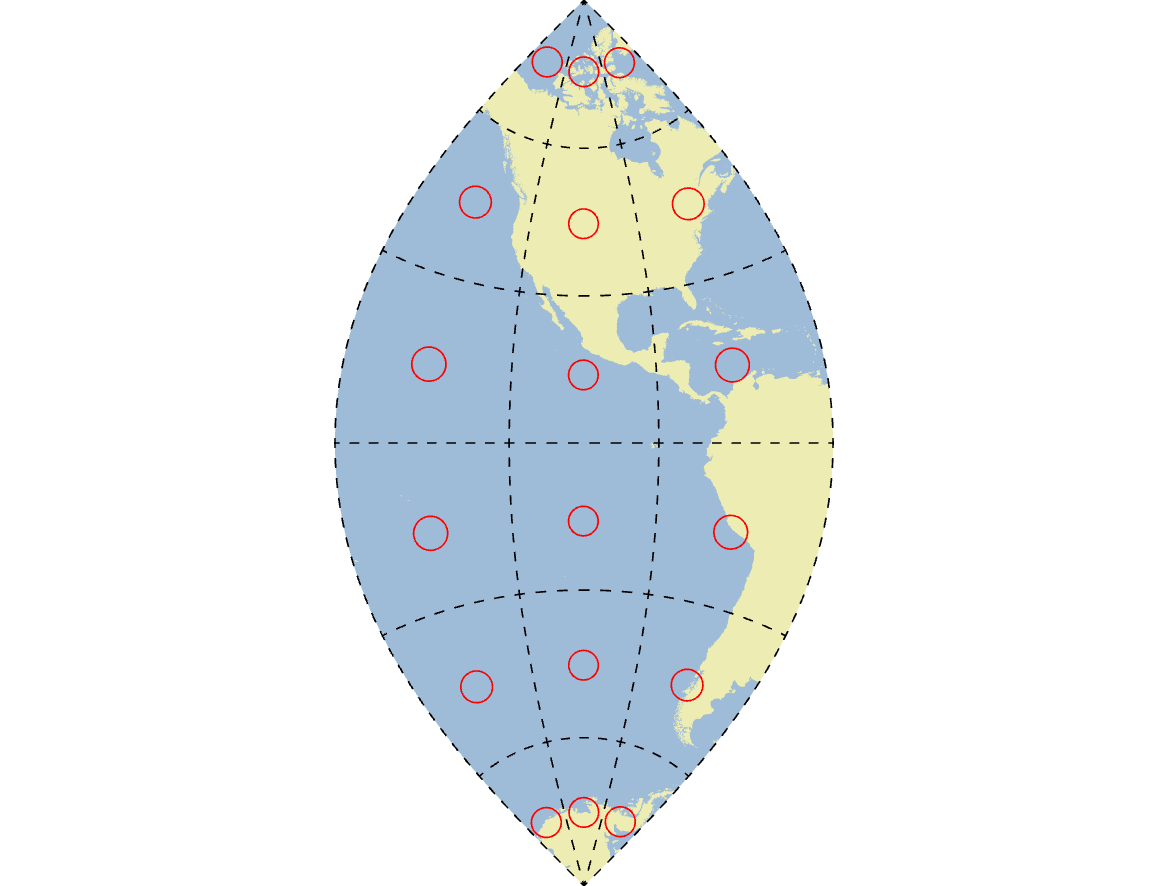
\includegraphics[width=0.75\linewidth]{images/02-UTM-13N-map} \caption{Universal Transverse Mercator Zone 13 map projection with Tissot's Indicatrices in red. Pickell, CC-BY-SA-4.0.}\label{fig:2-UTM-13N-map}
\end{figure}

Besides defining the orientation of the cylinder, we can also specify its size or diameter. When the diameter of the cylinder is equivalent to the diameter of Earth at the Equator, a single tangent line is formed. If the diameter of the cylinder is smaller than Earth's diameter at the Equator, then the cylinder has two lines that contact Earth's surface, known as \textbf{secants}. The purpose for having two secants is that the projection distortion can be more evenly distributed across the map. In the case of UTM, a scale factor of 0.9996 is applied to shrink the transverse cylinder slightly, forming two secants that are 360 km apart East-West. In between the two secants lies the \textbf{central meridian}, which is used to define the origin for the projected coordinate system. It is important to realize that the secants are parallel to each other and the central meridian, which means the secants are not meridians on Earth and form what are called \textbf{small circles}, a line that does not divide Earth into two equal portions.

UTM uses a unique coordinate system that deserves some explanation. Just like with latitude and longitude coordinates \([λ,φ]\), an arbitrary origin needs to be defined so that we know where we are in relation to the origin on the map. For projected coordinate systems like UTM that use linear units of measure such as meters, the origin is defined as the intersection of the central meridian and the Equator. Simple enough, right? There is one catch: UTM does not use any negative coordinates by convention. Thus, the origin of the coordinate system for each zone must be moved so that coordinates West of the central meridian and South of the Equator are positive. To do this, a constant value is added to all East-West coordinates (known as \textbf{Eastings}) and all North-South coordinates (known as \textbf{Northings}) to create what are known as \textbf{False Eastings} and \textbf{False Northings}, respectively. A value of 500,000 m is added to all Eastings so that the western limit of the zone is located at 0 m, the central meridian is located at 500,000 m, and the eastern limit of the zone is located at 1,000,000 m. A value of 10,000,000 m is added to all Northings in the Southern Hemisphere so that the Equator is at 10,000,000 m and 0 m is near the South Pole for all southern UTM zones. You might recognize the importance of the 10,000,000 m value because this represents approximately one-quarter of the Earth's North-South circumference.

\subsection{Sinusoidal}\label{sinusoidal}

Sinusoidal is a \emph{pseudocylindrical} map projection, so-named because these projections approximate a true cylindrical projection except that Meridians are curved instead of straight like with Mercator or UTM. Because Meridians are curved, Sinusoidal maps represent the North and South Poles as single points instead of lines as is the case with Mercator. Thus, Sinusoidal maps are not conformal and distort shape, but they are in fact equal-area (Figure \ref{fig:2-Sinusoidal-map}). Equal-area map projections like Sinusoidal are important for accurately accounting for land cover and other global mapping efforts. Therefore, it is common to find global datasets distributed in a Sinusoidal map projection.

\begin{figure}
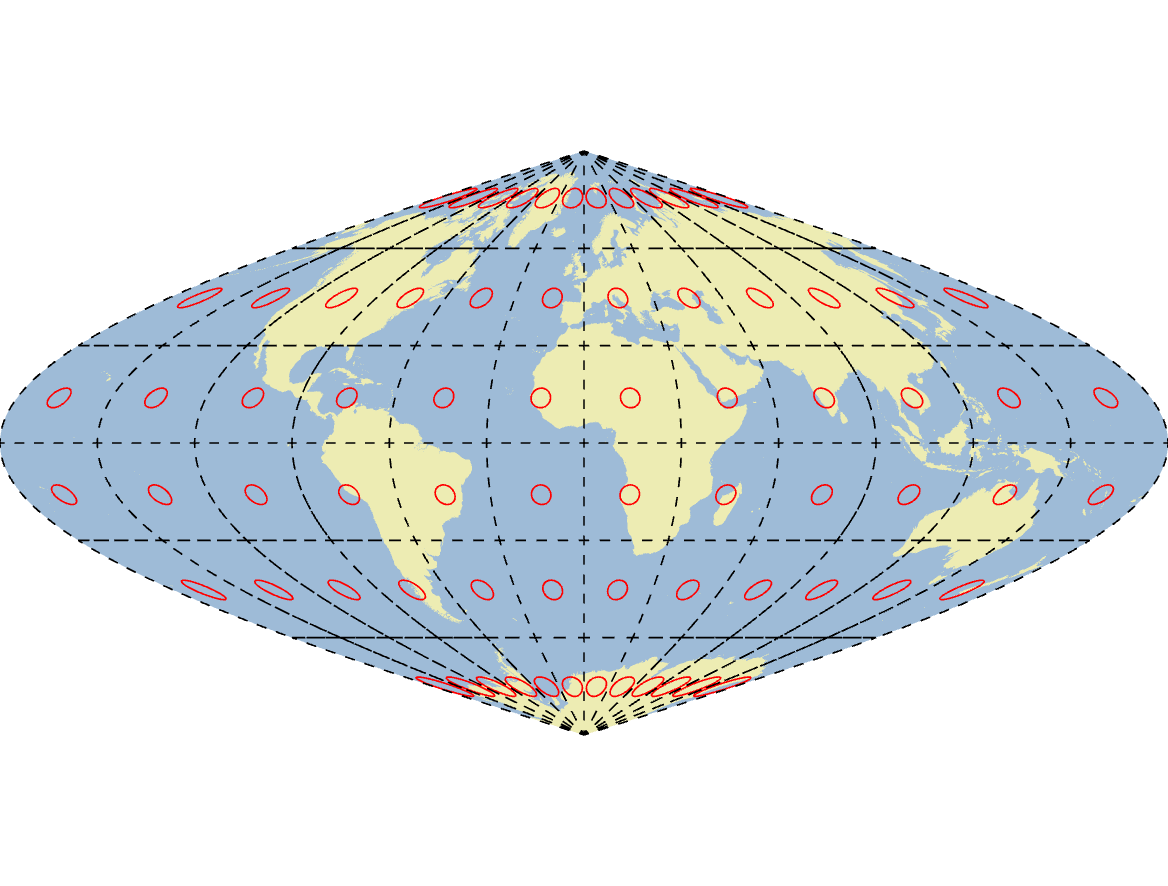
\includegraphics[width=0.75\linewidth]{images/02-Sinusoidal-map} \caption{Sinusoidal map projection with Tissot's Indicatrices in red. Pickell, CC-BY-SA-4.0.}\label{fig:2-Sinusoidal-map}
\end{figure}

\subsection{Albers}\label{albers}

Albers is another example of an equivalent map projection, but unlike Sinusoidal, an Albers projection uses a cone as a projection surface instead of a pseudocylinder. Like the cylindrical case, the cone can be sized and oriented in any way, but the cone of an Albers projection is typically oriented so that the vertex of the cone aligns with the rotational axis of Earth. The base of the cone has a diameter that usually results in two secants, known as \textbf{standard parallels} on an Albers map. Thus, Albers projections tend to distort latitudinally as you move North-South away from the standard parallels, but even more so as you move toward the base of the cone (Figure \ref{fig:2-BC-Albers-map}). Besides being an equal-area projection, Albers is a good choice for mapping regions because shape and scale are mostly preserved near the standard parallels. For example, the province of British Columbia has adopted a modified Albers projection that situates the standard parallels at 50° N and 58.5° N, which are near the northern and southern latitudinal limits of the province. This narrow band of latitude between the standard parallels ensures that there is relatively little distortion in shape and scale within the province, which is comparable to UTM. However, British Columbia is a longitudinally wide province, spanning 6 of Canada's 15 total UTM zones, so Albers has a distinct advantage of being able to show the entire province with little distortion. For the same reasons, you will often find Canada-wide data distributed in an Albers projection.

\begin{figure}
\includegraphics[width=0.75\linewidth]{images/02-BC-Albers-map} \caption{British Columbia Environment Albers map projection with Tissot's Indicatrices in red. Pickell, CC-BY-SA-4.0.}\label{fig:2-BC-Albers-map}
\end{figure}

\subsection{Azimuthal}\label{azimuthal}

Azimuthal projections use a flat circular plane to project the Earth onto a map. This plane is usually oriented so that it is tangent at a single point, usually the North or South Pole. In the case of a polar azimuthal projection, meridians radiate outward as straight lines from the pole to the edge of the circular plane and the parallels are represented as concentric circles. As a result, distortion increases as you move away from the centre point of the map with the outer edge of the plane representing an \textbf{antipode} or an opposite point on Earth. The primary benefit of azimuthal projections is that they preserve direction and distance between the centre point and any other point in the map (Figure \ref{fig:2-Azimuthal-map}). The shortest geographic distance between the centre point and any other point creates a line known as a \textbf{great circle}, which divides the Earth into two equal portions. So another benefit of an Azimuthal project is that great circles can be mapped as straight lines. Azimuthal projections are commonly used when distance and direction are important, such as weather RADAR stations or air traffic control towers. It is important to realize that the centre point for an azimuthal projection can be any point on Earth and the equidistant property can be exploited for a number of applications.

\begin{figure}
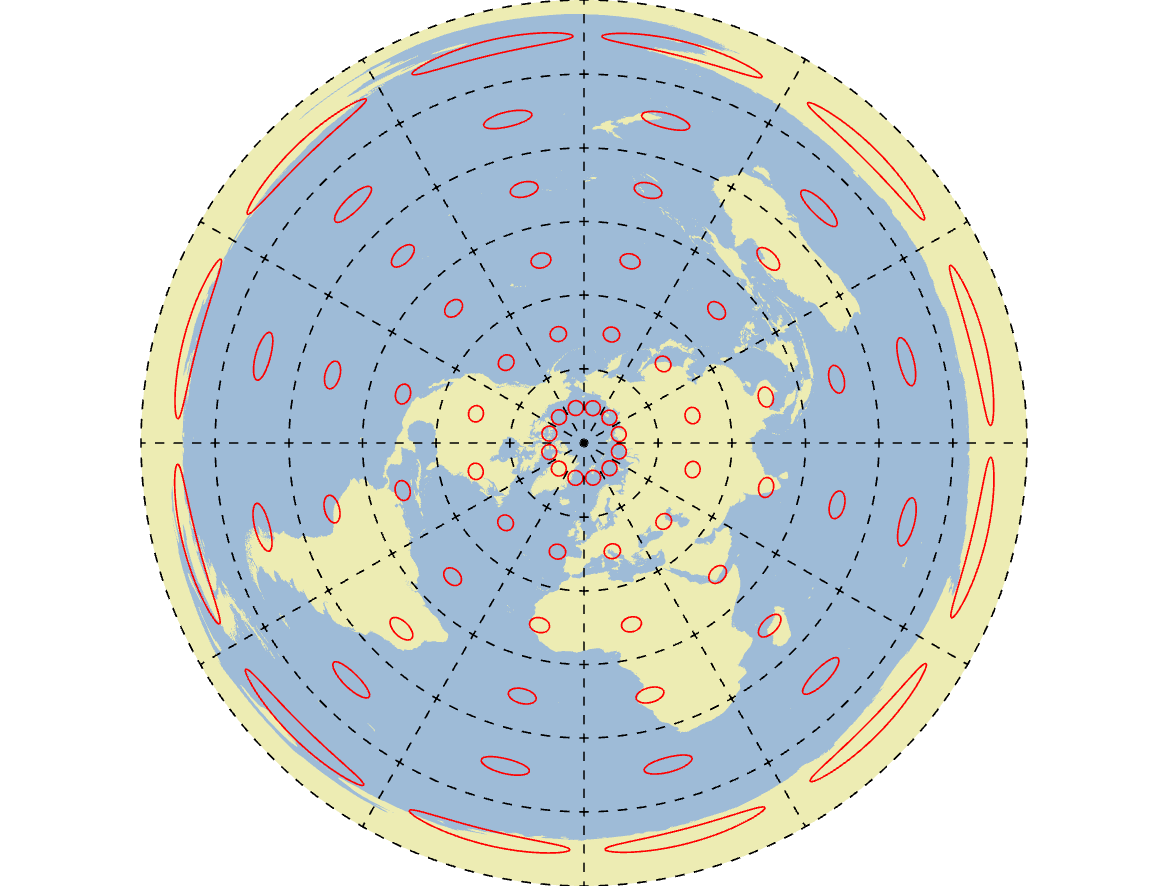
\includegraphics[width=0.75\linewidth]{images/02-Azimuthal-map} \caption{North Pole Azimuthal map projection with Tissot's Indicatrices in red. Pickell, CC-BY-SA-4.0.}\label{fig:2-Azimuthal-map}
\end{figure}

\section{Summary}\label{summary-1}

In this chapter, you learned about the science and technology of geodesy that goes into mapping data. We described the different models of Earth's shape and the advantages and disadvantages that each model has. More generally, models of Earth represent vertical datums to which heights are referenced. When we think of ``where'' something is on Earth, we must use horizontal datums to reference location. There are two types of horizontal datums that are very important to geomatics: (1) a geographic coordinate system uses lines of latitude and longitude to define locations on Earth's 3-dimensional surface while (2) a projected coordinate system flattens Earth into a manageable 2-dimensional coordinate space. In the case of projected coordinate systems, we have many choices when deciding which map projection to use when we map data, each with its own uses and distortions. The next time that you look at a map, ask yourself with your new found appreciation of geodesy, how is this information being misrepresented to me?

\section*{Reflection Questions}\label{reflection-questions-1}
\addcontentsline{toc}{section}{Reflection Questions}

\begin{enumerate}
\def\labelenumi{\arabic{enumi}.}
\tightlist
\item
  Describe the process of measuring the height of something on Earth.
\item
  Explain the difference between a geographic coordinate system and a projected coordinate system.
\item
  Name as many projected coordinate systems as you can.
\end{enumerate}

\chapter{Data Types and Spatial Data Models}\label{types-of-data}

Written by
June Skeeter and Paul Pickell

In the previous chapter, we discussed some of the unique challenges associated with representing spatial data in a GIS, and how to account for these these with geographic coordinates systems and map projections. In this chapter we will discuss more broadly how to represent both spatial and non-spatial data in a Geographic Information System. We will introduce the different types of data that can represent non-spatial attributes and discuss the different scales this data can be measured on. Then we will introduce the different \emph{spatial data models} we use to link the spatial and non-spatial data. Finally, we will cover some of the different file types that can be used to store data.

\subsection*{Learning Objectives}\label{learning-objectives-2}
\addcontentsline{toc}{subsection}{Learning Objectives}

\begin{enumerate}
\def\labelenumi{\arabic{enumi}.}
\tightlist
\item
  Types of Spatial Phenomena
\item
  Measurement Scales of Data: Quantitative vs.~Qualitative
\item
  Overview of Raster and Vector Data Models
\item
  Data Resolutions
\item
  Common File Types in GIS
\end{enumerate}

\subsection*{Key Terms}\label{key-terms-2}
\addcontentsline{toc}{subsection}{Key Terms}

Phenomena, Discrete Object, Continuous Field, Qualitative, Quantitative, Measurement Scale, Raster, Vector, Resolution,

\section{Types of Phenomena}\label{types-of-phenomena}

\textbf{Phenomenon}, noun, plural \emph{Phenomena}: \emph{1} a fact or situation that is observed to exist or happen, especially one whose cause or explanation is in question. \emph{2} a remarkable person, thing, or event \citep{oxford_languages_phenomena_nodate}. Essentially, anything and everything are phenomenon: lightning, a country, coastlines, a dog on a kayak. Broadly speaking, in GIS we categorize phenomena as \textbf{discrete} or \textbf{continuous}. Both kinds of phenomena can be represented in a GIS, but they come with different considerations and cannot always be represented with the same kind of data model.

\begin{figure}
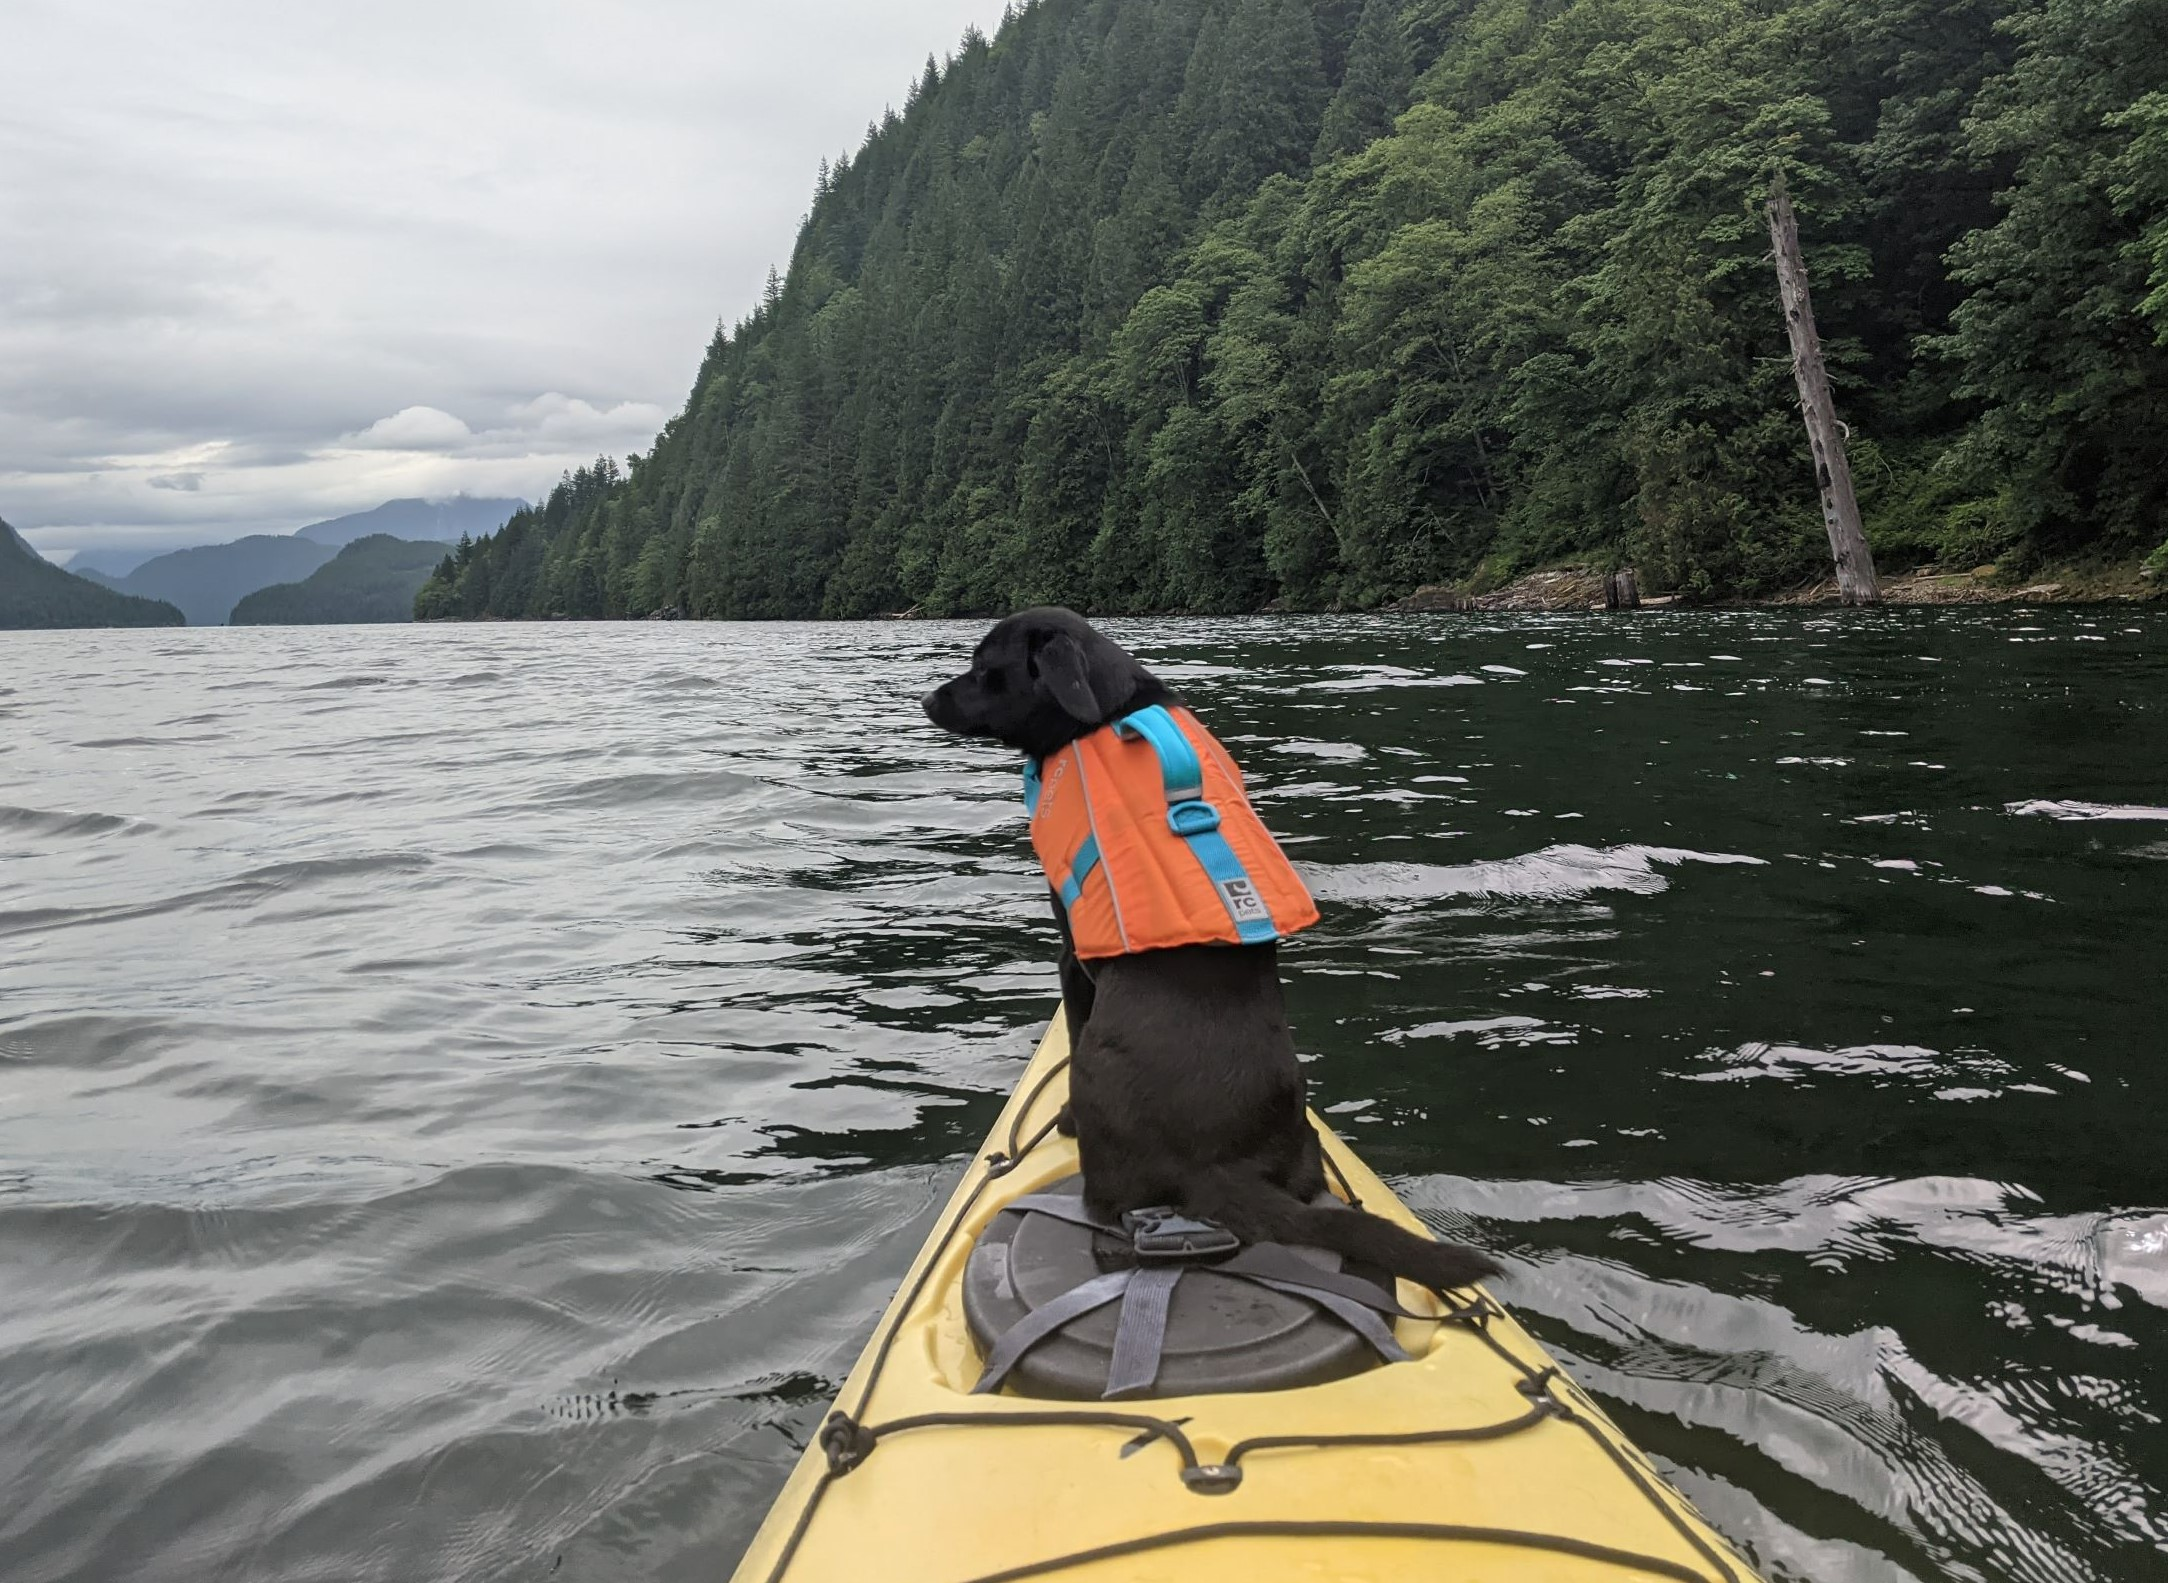
\includegraphics[width=0.75\linewidth]{images/03-dog-on-a-boat} \caption{Yarrow enjoying the scenery at Aloutte Lake, she's quite the phenomenon indeed. Skeeter, CC-BY-SA-4.0.}\label{fig:3-dog-on-a-boat}
\end{figure}

\subsection{Discrete Objects}\label{discrete-objects}

Discrete objects are finite and have distinct boundaries. Each object is a unique, self contained entity whose geography can be exactly defined. Because each object is unique and self contained, collections of objects are countable. A concrete example of a discrete objects would be buildings. They are real physical objects with well defined boundaries. We can count the number of buildings on a college campus or in a city. National and sub-national boundaries are also discrete objects. They (typically) have well defined boundaries and we can easily count the number of nations or provinces. They are not, however, real physical objects. Political boundaries are arbitrary human constructs.

\begin{figure}
\includegraphics[width=0.75\linewidth]{images/03-vector} \caption{Provinces are clearly delineated, distinct objects, despite having no real physical presence. Skeeter, CC-BY-SA-4.0.}\label{fig:3-vector}
\end{figure}

\subsection{Continuous Fields}\label{continuous-fields}

Continuous fields are infinite and lack defined boundaries. Fields can be measured at an infinite number of locations. However, similar values tend to cluster in space so we can often make assumptions based on finite observations of continuous fields. One of the most common examples of a continuous field is elevation. This is a physical property associated with every location on earth. We can't count the ``number of elevations'' because space is infinitely divisible and everywhere in space can have an elevation.

\begin{figure}
\includegraphics[width=0.75\linewidth]{images/03-elevation} \caption{Elevation of the Sunshine Coast in BC, from the NRCAN DEM (google earth engine) [@nrcan_canadian_2021]}\label{fig:3-elevation}
\end{figure}

\subsection{Imperfect Distinctions}\label{imperfect-distinctions}

Few phenomena will fit perfectly and exclusively into one category or the other. That said, its helpful for us to think about the discrete v. continuous dichotomy. As long as we recognize that it's not a perfect classification. Whether a phenomenon is considered discrete or continuous depends on scale (both spatial and temporal) and perspective. Some phenomenon are a bit of both. Take the coastlines, they can be treated as discrete or continuous. At the scale of an individual beach over hours, tides can cause wide variations in water levels/position. How/where does one draw the discrete line representing the ``coast''. At this scale, the coast isn't really a discreet object, rather a continuous field known as the inter-tidal zone. Zoom out a bit and those fluctuations aren't particularly relevant if you want to make a map of Pacific Rim National Park. The coast could be considered a discrete object. But if you change the timescale and look at sea level rise projections, then you're dealing with a continuous field.

\begin{figure}
\includegraphics[width=0.75\linewidth]{images/03-beach-small-scale} \caption{The west coast of Vancouver Island. Skeeter, CC-BY-SA-4.0.}\label{fig:3-beach-small-scale}
\end{figure}

A lightning strike is an electric discharge between the atmosphere and the ground. A lightning strike is a discrete object. The precise location of the strike can be pin pointed, the number of strikes during a storm can be counted. But what about the actual lighting bolt? That's more a continuous field, its not really possible to measure the exact boundaries of the path the electric discharge takes. Then we can look at other things, like the probability of lighting strikes. Figure \ref{fig:3-lightning-density} is a continuous field, calculated from counting discrete objects.

\begin{figure}
\includegraphics[width=0.75\linewidth]{images/03-lightning-density} \caption{Global lighting strike density per month. Skeeter, CC-BY-SA-4.0.}\label{fig:3-lightning-density}
\end{figure}

\section{Types of Data}\label{types-of-data-1}

Within the context of a Geographic Information System, each piece of information pertaining to a phenomena can be referred to as an \textbf{Attribute}. An phenomena can have many different attributes associated with it, but each attribute can broadly be said to address one of three questions: \textbf{What}, \textbf{When}, or \textbf{Where}? Attributes that describe \emph{where} are known as \textbf{Spatial Data} while all other attributes are \textbf{Non-Spatial Data}. All data, spatial and non-spatial, can broadly be classified as either \textbf{qualitative} or \textbf{quantitative}. These data types are fundamentally different and are therefore measured on fundamentally different scales. The types of analysis we can conduct with qualitative data are more limited than quantitative data, but that does not necessarily mean quantitative data are ``better'' than qualitative.

\begin{figure}
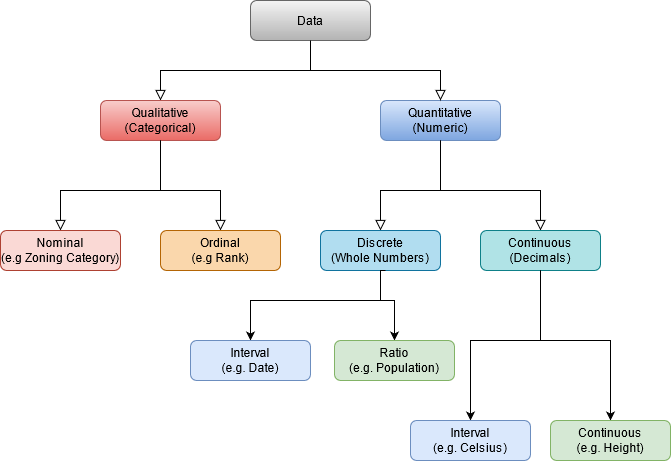
\includegraphics[width=0.75\linewidth]{images/03-data-types} \caption{Summary of the types of data. Skeeter, CC-BY-SA-4.0.}\label{fig:3-data-types}
\end{figure}

\subsection{Qualitative Data}\label{qualitative-data}

Qualitative data are categorical; they are strictly descriptive and lack any meaningful numeric value. They describe the qualities of a phenomenon, without giving us any numeric information. Most qualitative data you will work with in GIS are textual or coded numerals, but there are circumstances where you may encounter non-textual data (e.g.~images, sound clips, videos) in a dataset. Qualitative data can be ``spatial'' in nature (e.g.~relative directional descriptors: left/right, near/far, north/south), but because they lack numeric values, they cannot be used for spatial analysis. Qualitative data can be measured on either a \textbf{Nominal} or \textbf{Ordinal} scale.

\subsubsection{Nominal Scale}\label{nominal-scale}

These are data that just consist of names or categories with no ranking or direction are nominal. One category is not more or less, better or worse than another, they are just different. A good example would be flower types. Other examples would be zoning categories, colors, flavors of ice cream, place names, etc. With nominal data, you can check for equality between entities and you can count occurrence. These are the only operations we can do. You can't calculate

\begin{figure}
\includegraphics[width=0.75\linewidth]{images/03-flowers-nominal} \caption{Each flower is different, but no flower is 'more' or 'less' a flower than any of the others. Skeeter, CC-BY-SA-4.0.}\label{fig:3-flowers-nominal}
\end{figure}

\begin{figure}
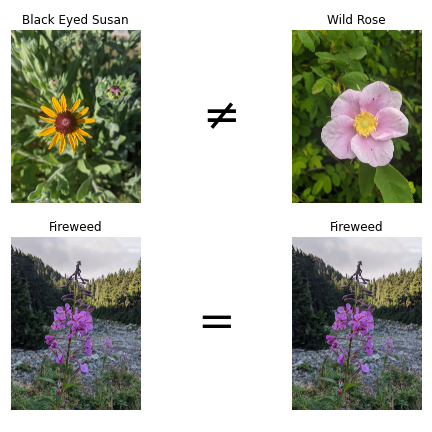
\includegraphics[width=0.75\linewidth]{images/03-nominal-operations} \caption{Checking equality with flower species. Skeeter, CC-BY-SA-4.0.}\label{fig:3-nominal-operations}
\end{figure}

\subsubsection{Ordinal Scale}\label{ordinal-scale}

Ordinal scale data are categories that also have a some ranking or directionality. A good example would be relative sizes (see Figure \ref{fig:3-dogs-ordinal}). Some other good examples of ordinal data include spice levels (mild, medium, hot), residential zoning density (low, medium, high), and survey responses.

\begin{figure}
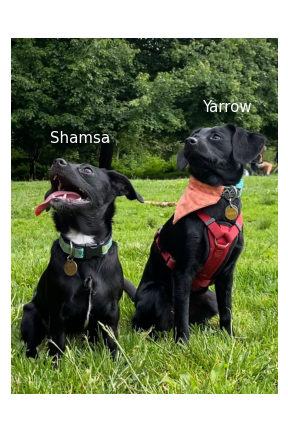
\includegraphics[width=0.75\linewidth]{images/03-dogs-ordinal} \caption{We can see Yarrow is taller than her sister Shamsa, so we can rank these dogs by height. However, we haven't measured their heights, so we don not know how much taller Yarrow is than Shamsa. Skeeter, CC-BY-SA-4.0.}\label{fig:3-dogs-ordinal}
\end{figure}

\begin{figure}
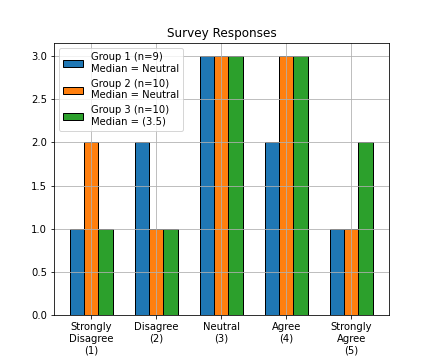
\includegraphics[width=0.75\linewidth]{images/03-ordinal-operations} \caption{In some circumstances, we can directly calculate the median (middle value) of an ordinal set. With odd numbered sets (e.g. Group 1), the median is simply the middle value of the set, when sorted lowest to highest. We can always take the median when we have an odd number.  With even numbered sets, its a bit more complicated.  The median, is the average of the middle two values. For Group 2, the middle values (5th and 6th) are both 'Neutral', so we don't have an issue. But for Group 3, the 5th value is 'Neutral' and the 6th value is 'Agree'. We cannot directly average these two ordinal values. One solution is to arbitrarily assign a numeric score to the ordinal categories (e.g., 1-5). This would then allow you to show the median is between 'Neutral' and 'Agree'. Skeeter, CC-BY-SA-4.0.}\label{fig:3-ordinal-operations}
\end{figure}

The only arithmetic operations we can do with nominal data are checking for equality (True/False), counting occurrences (frequencies), and calculating the mode (most frequent occurrence). With ordinal data, we can do these operations as well, plus a few more. We can check the order/rank (greater than, less than) and in some circumstances we can calculate the median (see Figure \ref{fig:3-ordinal-operations}).

(Graded Membership) When trying to group real world phenomena into categories, there are often ``exceptions'' that blur the lines a bit. Take this example: you are trying to develop a land cover classification scheme for Garibaldi Provincial park in British Columbia. Some of the land surface is unquestionably alpine tundra and some is certainly forest area. However, the transition between forest and alpine meadow is not an abrupt line. How/where do you draw the line? Examples like this are known as fuzzy variables, and we often use a \emph{Graded Membership} scale to assign them to categories. With the landscape classification, a simple approach would be a ``winner take all'' approach. If a plot is 5\% bare rock, 40\% forest, and 45\% alpine meadow, the area will be classified as alpine meadow. From that point forward, in the GIS, that area will be treated as alpine meadow, any information about the variability within the area will be lost. In practice, many of the qualitative data we work with in GIS, especially those describing natural phenomena, are actually graded membership variables.

\begin{figure}
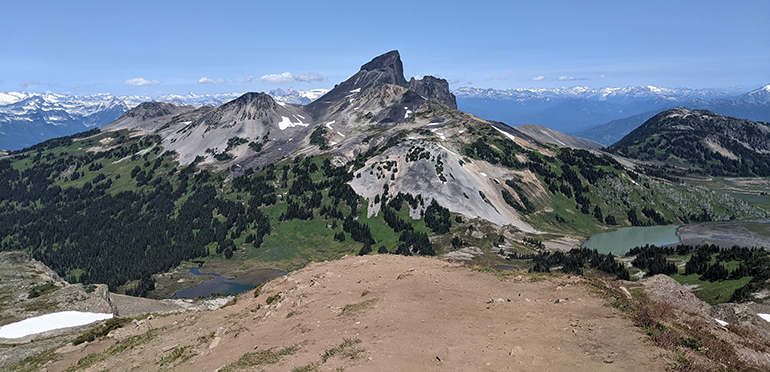
\includegraphics[width=0.75\linewidth]{images/03-fuzzy} \caption{In this example, we see an alpine landscape in Garibalid Provinical Park, BC.  We can see patches of forest and patches of meadow.  But where, exactly, would we draw the boundary between these two landscape classes. Skeeter, CC-BY-SA-4.0.}\label{fig:3-fuzzy}
\end{figure}

\subsection{Quantitative Data}\label{quantitative-data}

Quantitative data are numeric; they describe the quantities associated with an phenomena. The numerical values that are separated by a unit that has some inherent meaning (as opposed to the arbitrary numeric codes like in the ordinal data example). This allows us to conduct a wider range of arithmetic operations on quantitative data. In addition to the operations we perform on Qualitative data; with numeric data we can always calculate measures of central tendency (mean/median) and we can add/subtract values to calculate differences.

Numeric data can be either \textbf{discrete} or \textbf{continuous}. Discrete variables (e.g.~population) are obtained by counting and values within a range cannot be infinitely subdivided. You can have a population of 1, 37, or 179 but you cannot have a population of 2.3. Continuous variables (e.g.~temperature) can take an infinite number of values a given range, but they cannot be counted. You can have temperatures of 10, 10.5, or 10.1167 °C, but a temperature of 10°C does not mean you have 10 individual degrees of temperature. Quantitative data (both discrete and continuous) can be measured on either an \textbf{Interval} or \textbf{Ratio} scale. These types of quantitative data are closely related, but have one important distinction.

\subsubsection{Ratio Data}\label{ratio-data}

Ratio data have fixed, meaningful, absolute zero points. The absolute zero point means ratio data cannot take negative values. It also means that we can multiply/divide two values to calculate a meaningful ratio between them (hence the name). A good example of ratio data are population total (see figure). Population counts start at zero and go up from there. A population of zero means there are no residents, and its impossible to have a negative population. Other examples of ratio data include: temperature (\emph{in degrees Kelvin}), precipitation, tree height, income, rental cost, and units of time (years, seconds, etc.)

\begin{figure}
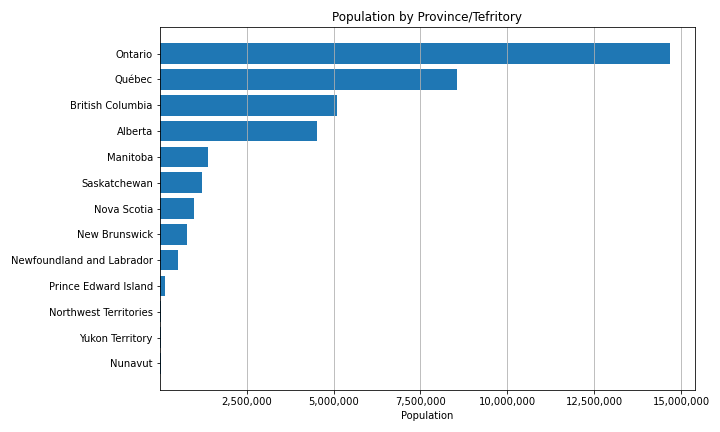
\includegraphics[width=0.75\linewidth]{images/03-ratio-population} \caption{Because of the fixed, meaningful zero point, we can calculate ratios between populations: e.g. Manitoba's population is 1/10th that of Ontario, British Columbia has 129 times as many people as Nunavut. Skeeter, CC-BY-SA-4.0.}\label{fig:3-ratio-population}
\end{figure}

Interval data on the other hand, have an arbitrarily set zero point. This means they can can take negative values. Because the zero point is arbitrary, we cannot multiply/divide two values or calculate meaningful ratios between two values. A good example of interval data is temperature measured in Celsius, and comparing it to Kelvin highlights the difference between the two data types (see Figure \ref{fig:3-interval-ratio-temperature}). The conversion between Kelvin (ratio) and Celsius (interval) is very simple: °C = °K-273.15. Zero Kelvin is ``Absolute Zero'' - ie. the lack of temperature, while zero Celsius is the freezing point of water (273.15 degrees above absolute zero). Other examples of interval data include: the pH scale, IQ test scores, elevation (relative to a datum) dates (April 12th, 2011), and times (11:00 A.M.).

\begin{figure}
\includegraphics[width=0.75\linewidth]{images/03-interval-ratio-temperature} \caption{The ratio between two temperatures in Celsius is not meaningful, 20&deg;C is not 'twice' as warm as 10&deg;C. Kelvin's zero point is fixed to absolute zero, the 'absence' of temperature.  So we can calculate the ratio, 293.15&deg;K is 1.035 times warmer than 283.15&deg;K. Skeeter, CC-BY-SA-4.0.}\label{fig:3-interval-ratio-temperature}
\end{figure}

\subsection{Derived Ratio: Normalizing Data}\label{derived-ratio-normalizing-data}

Sometimes we want to account for the influence of one variable when analyzing another. To do this, we can divide one value by by another to get the ratio of the two, also known as a \textbf{derived ratio}. This process is sometimes referred to as \textbf{Normalizing} or \textbf{Standardizing} our data. The basic formula is: \(C=\frac{A}{B}\), where A is our variable of interest, B is our confounding variable, and C is our new derived ratio. There are many circumstances where we might need to do this. One common example is population density: Canada and Poland both have populations of \textasciitilde{} 38 million people but Canada had 32x the land area of Poland. Any comparison of the these two nations that fails to account for the size disparity would be seriously flawed. Another key example are affordability indexes. The example below shows how normalization can be applied to a households expenditures on food. Income and household expenditures on food are strongly related (wealthy regions tend to purchase more expensive food). An analysis of the cost of food that doesn't account for this relationship would not adequately account for the \emph{affordability} of food in a given region. Dividing household food expenditures by household income, we get the proportion of income spent on food. This is a much more accurate representation of the affordability of food and highlights that the poorest communities are most severely impacted by increasing food costs.

\begin{figure}
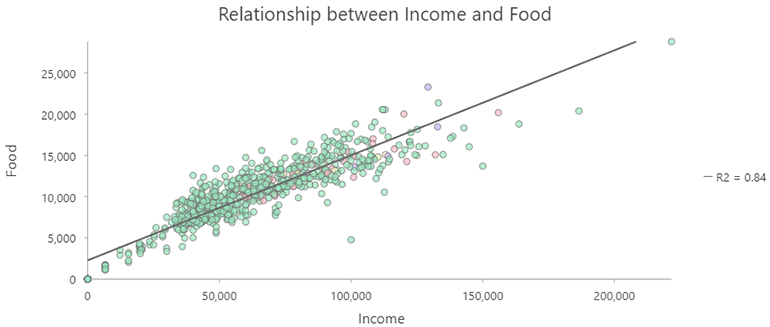
\includegraphics[width=0.75\linewidth]{images/03-income-v-food} \caption{Income vs. household expenditures on Food by Census Subdivisions in BC. Skeeter, CC-BY-SA-4.0.}\label{fig:3-income-v-food}
\end{figure}

\begin{figure}
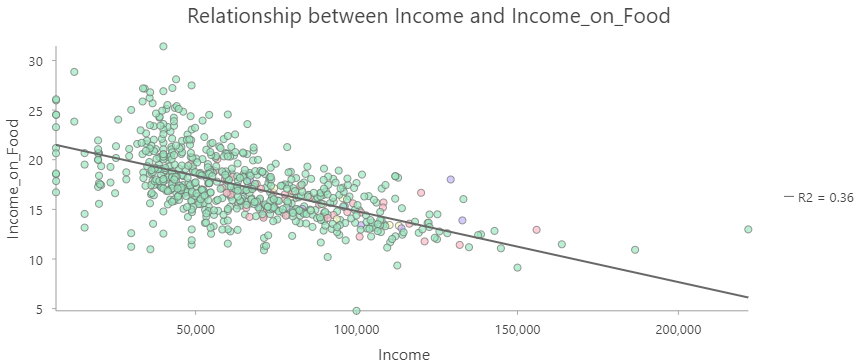
\includegraphics[width=0.75\linewidth]{images/03-income-v-income-on-food} \caption{Income vs. Fraction of Income Spent on Food by Census Subdivisions in BC. Skeeter, CC-BY-SA-4.0.}\label{fig:3-income-v-income-on-food}
\end{figure}

\subsection{Summary of Data Types}\label{summary-of-data-types}

\begin{longtable}[]{@{}lllll@{}}
\toprule\noalign{}
Operation & Nominal & Ordinal & Interval & Ratio \\
\midrule\noalign{}
\endhead
\bottomrule\noalign{}
\endlastfoot
Equality & x & x & x & x \\
Counts/Mode & x & x & x & x \\
Rank/Order & & x & x & x \\
Median & & x & x & x \\
Add/Subtract & & & x & x \\
Mean & & & x & x \\
Multiply/Divide & & & & x \\
\end{longtable}

\section{Spatial Is Special}\label{spatial-is-special}

You might encounter the phrase ``Spatial is special'' in your time studying GIS. Spatial data is the foundation of Geographic Information Science, it is what distinguishes GIS from the broader field of data science. This was succinctly summarized by Waldo Tobler in The First Law of Geography:
- \emph{``Everything is related to everything else, but near things are more related than distant things.''}

\begin{figure}
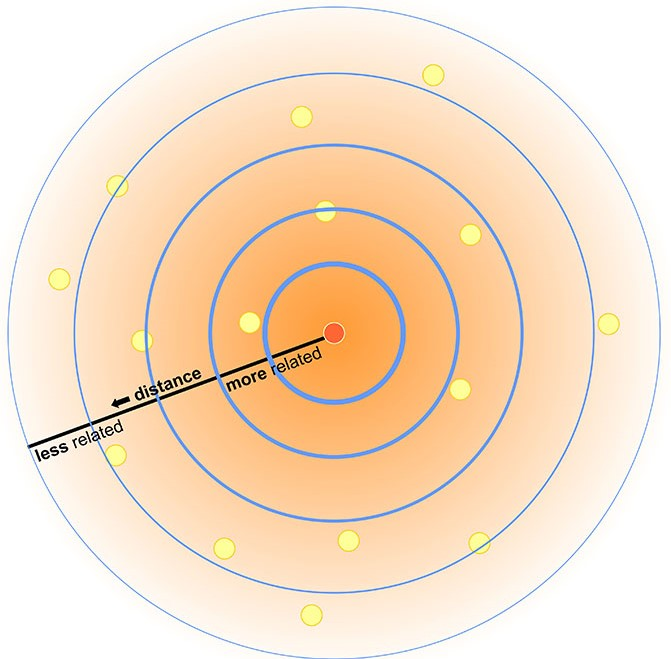
\includegraphics[width=0.75\linewidth]{images/03-spatial-is-special} \caption{Visualization of Tobler's First Law. Skeeter, CC-BY-SA-4.0.}\label{fig:3-spatial-is-special}
\end{figure}

This might seem obvious: people interact more if they live in the same city, orca pods in different areas develop different dialects, hemlocks on Vancouver Island are more related to their neighbors than to to hemlock in the New Brunswick. Generally, near things are more related to one another, but it \emph{does not guarantee similarity}. Downtown Vancouver averages 40 cm of snow/year, but the ski resort on Grouse Mountain 15 km north gets over 9 m. These locations are impacted by the same storm systems, but the 1200 m elevation difference causes vastly different quantities and different types of precipitation.

The measure of similarity between objects across space called \textbf{spatial autocorrelation}. Spatial autocorrelation allows us to make some a key assumptions when representing spatial data. We don't have to measure a phenomena everywhere in order to represent it adequately. We only need to measure it at specific locations or over regular intervals. If point A is in dense forest, it is likely point B 10 m away is also in a dense forest. We do not have to get the location of every tree in the forest. Instead, we can look at the average presence of trees over a larger area.

\begin{figure}
\includegraphics[width=0.75\linewidth]{images/03-bc-snow} \caption{Screengrab from Hectares BC, can easily make into better map. Skeeter, CC-BY-SA-4.0.}\label{fig:3-bc-snow}
\end{figure}

\section{Spatial Data Models}\label{spatial-data-models}

As discussed in the previous chapter, spatial data is three-dimensional, though we usually project it into two-dimensions for simplicity. Because of the unique transformations that must be applied to spatial data, it must be treated and represented differently than the non-spatial data that describe \emph{what} is happening and \emph{when}. We cannot simply put all of our data into a spreadsheet and start analyzing it. We have to use \textbf{Spatial Data Models} to organize our data and link our spatial and non-spatial data. Spatial data models store geographic data in a systematic way so that we can effectively display, query, edit, and analyze our data within a GIS.

There are two main types of spatial data models: the \textbf{Raster} and \textbf{Vector} models. The raster data model represents spatial data as grid of cells, and each cell has one non-spatial attribute associated with it. The vector data model represents spatial data as either points, lines, or polygons that are each linked to one or more non-spatial attributes. These two models represent the world in fundamentally different ways. One is not inherently better than the other, but they are better suited for different circumstances. The choice of which model to use is often dictated by three main factors:

\begin{enumerate}
\def\labelenumi{\arabic{enumi})}
\tightlist
\item
  The type of phenomena we are trying to represent.
\item
  The scale at which we plan to analyze our data.
\item
  How we plan to use the data.
\end{enumerate}

\begin{figure}
\includegraphics[width=0.75\linewidth]{images/03-vector-v-raster} \caption{Representing space in the raster model vs. the vector model. Skeeter, CC-BY-SA-4.0.}\label{fig:3-vector-v-raster}
\end{figure}

\subsection{Raster Data Model}\label{raster-data-model}

The raster data model represents a phenomena across space as a gridded set of cell (or pixels). The cell size determines the \textbf{Resolution} of the raster image, that is the smallest feature we can resolve with the raster. A 10 m resolution raster has cells that are 10 x 10 m (100 m2), a 2 m resolution has cells that are 2 x 2 m (4 m2). Along with the cell size, the number of rows and columns dictates the extent (or bounds) of a raster image. A raster with a 1 m cell size, 5 rows, and 5 columns, will cover an area of 5 m x 5 m (25 m2). Because of the full coverage within their bounds, raster data models are very well suited for representing \emph{continuous phenomena} where cell values correspond to measured (or estimated) value at specific location. In GIS, rasters are commonly encountered as: satellite and drone imagery, elevation models, climate data, model outputs, and scanned maps.

\begin{figure}
\includegraphics[width=0.75\linewidth]{images/03-raster-example} \caption{Example of raster data. Skeeter, CC-BY-SA-4.0}\label{fig:3-raster-example}
\end{figure}

The value of a pixel can be quantitative (e.g.~elevation) or qualitative (e.g.~land use). Each pixel/cell can only have a single value associated with it. Multiple bands can be combined to store or more information, as is done with a RGB color photograph. Algebraic expressions can also be performed quickly and efficiently with raster layers a inputs. This is known as raster overlay, and is one of the key advantages to raster data. If layer A = Average July Temperature and layer B = Average January Temperature, then A -- B will give us the Average Temperature Range across the rasters domain.

\begin{figure}
\includegraphics[width=0.75\linewidth]{images/03-raster-overlay} \caption{Raster math illustration. Skeeter, CC-BY-SA-4.0.}\label{fig:3-raster-overlay}
\end{figure}

Rasters data relies on Spatial Autocorrelation and The First Law of Geography, the model assumes that \emph{all areas} within a given cell are equally represented by the cell value. Depending on the resolution of the raster and the scale of the task at hand, this may or may not be an effective assumption. If you are trying to represent the coastline of Nova Scotia, 100 m or even 1 km resolution cells will likely suffice (see Figure \ref{fig:3-raster-resolution}). However, 10 km cells severely degrade the quality of the representation and at a 100 km cell size, the province is indistinguishable.

\begin{figure}
\includegraphics[width=0.75\linewidth]{images/03-raster-resolution} \caption{Raster Resolution. Skeeter, CC-BY-SA-4.0.}\label{fig:3-raster-resolution}
\end{figure}

The above example is related to something known as them \emph{mixed pixel} problem. Each cell in a raster can only have \textbf{one} value. So how do you handle when the area a cell covers contains \textbf{multiple} examples. Possible approaches are:

\begin{itemize}
\item
  \textbf{Majority/Mode}, the cell value is determined by the value/class covering the largest area within each cell. This can be useful for \textbf{discrete} phenomena, but generally will not be helpful for continuous phenomena.
\item
  \textbf{Touches All}, can be useful for discrete phenomena if you need to prioritize specific class(es) you can designate it them to be assigned to any pixel the touch (e.g., with flood/fire risk or most other hazards, you want to take an inclusive approach when defining risk zones. Better safe than sorry.)
\item
  \textbf{Nearest Neighbor/Center Point}, the cell value is determined by the value/class only at the center point of the cell. This method is quick to calculate but can under- or over-estimate repeating phenomena with frequencies lining up with the raster resolution (e.g., City Blocks/Roads, rows in agricultural fields).
\item
  \textbf{Average}, when working with continuous phenomena (e.g., rainfall, temperature, elevation) it might be best to use the average value across the cell instead. If multiple observations are available calculate the spatially weighted average within each cell. If we are working with discrete phenomena, this method is generally less useful.
\end{itemize}

When the data resolution is very high, relative to the scale of the map/analysis, the specific choice of method will produce negligible differences. If you are working with a 25 m resolution land cover classification and doing a continental scale analysis, the improper attribution of boundary pixels will not have a huge impact on the results. If the data resolution is low relative to the scale of your analysis, the choice of method could have a significant impact on your results.

Raster data can come in many different formats. \textbf{GeoTIFF} which has the extension .tif is one of the most common. This format is based of the Tag Image File Format (TIFF), a common file type used by graphic artists and photographers. A TIFF file stores metadata (data about the data) as tags. For instance, your camera might store a tag that describes the make and model of the camera and another for the date the photo was taken when it saves a picture. A GeoTIFF is a standard .tif image format plus additional tags spatial tags denoting spatial information including:

\begin{itemize}
\tightlist
\item
  Extent (minimum x,y and maximum x,y)
\item
  Resolution (cell size)
\item
  Projection, Coordinate system, and datum
\end{itemize}

Other file types you will likely encounter when working with raster data include:

\begin{itemize}
\tightlist
\item
  \begin{enumerate}
  \def\labelenumi{\arabic{enumi})}
  \tightlist
  \item
    IMG - A proprietary image format commonly used by ESRI products
  \end{enumerate}
\item
  \begin{enumerate}
  \def\labelenumi{\arabic{enumi})}
  \setcounter{enumi}{1}
  \tightlist
  \item
    JPEG2000 - A geospatial version of the common .jpg image type
  \end{enumerate}
\item
  \begin{enumerate}
  \def\labelenumi{\arabic{enumi})}
  \setcounter{enumi}{2}
  \tightlist
  \item
    ASCII - An older human readable format (simple text file) with slower performance than the types listed above.
  \end{enumerate}
\end{itemize}

\subsection{Vector Data}\label{vector-data}

The vector data model is much more well suited to represent discrete phenomena than the raster data model. A vector feature is a representation of a discrete object as a set of x,y coordinate pairs (points) linked to set of descriptive attribute about that object. A vector feature's coordinates can consist of just one (x,y) pair to form a single point feature, or multiple points which can be connected to form lines or polygons (see Figure \ref{fig:3-vector-types}). The non-spatial attribute data is typically stored in a \textbf{Tabular} format separate from the spatial data, and it is linked using an index. One of the key advantages of the vector model is the ability to store and retrieve many attributes them quickly. In GIS, vector data are commonly encountered as: political boundaries, cenus data, pathways (road, trails, etc.), point location (stop sign, fire hydrant), etc.

\begin{figure}
\includegraphics[width=0.75\linewidth]{images/03-vector-types} \caption{Vector objects (points, lines, or polygons) are stored along with any number of attribute. Point, line, and polygon data are typically stored in separate files. Skeeter, CC-BY-SA-4.0.}\label{fig:3-vector-types}
\end{figure}

\textbf{Points} are ``zero-dimensional'', they have no length or width or area. A point feature is just an individual (x,y) coordinate pair representing a precise location, that has some linked attribute information. Points are great for representing a variety of objects, depending on the scale. Fire hydrants, light poles, and trees are suitable to be represented as points in almost any application. If you are making a map of mines in British Columbia, or cities across Canada, it is probably acceptable to just display them as points.

\begin{figure}
\includegraphics[width=0.75\linewidth]{images/03-vector-points} \caption{An example of point data showing locations of trees.  The points are labeled with their index (unique ID number) which correspoonds to the attribute table below which stores more information about eacht tree. Skeeter, CC-BY-SA-4.0}\label{fig:3-vector-points}
\end{figure}

\begin{longtable}[]{@{}rrrlrr@{}}
\toprule\noalign{}
index & Longitude (X) & Latitude (Y) & Name & Age & Height \\
\midrule\noalign{}
\endhead
\bottomrule\noalign{}
\endlastfoot
0 & 0.44 & 0.03 & Fir & 54 & 119 \\
1 & 0.55 & 0.71 & Fir & 29 & 56 \\
2 & 0.89 & 0.33 & Fir & 82 & 197 \\
3 & 0.18 & 0.02 & Fir & 46 & 98 \\
4 & 0.65 & 0.51 & Maple & 87 & 212 \\
5 & 0.43 & 0.81 & Maple & 73 & 172 \\
6 & 0.38 & 0.86 & Maple & 94 & 233 \\
7 & 0.68 & 0.04 & Cedar & 34 & 68 \\
8 & 0.15 & 0.13 & Cedar & 36 & 73 \\
\end{longtable}

\textbf{Lines} are one-dimensional, they have length, but no width and thus no area. A line consists of two or more points. Every line must have a start point and end point, they may also have any number of middle points, called vertices. A vertex is just any point where two or more lines meet. Lines are also great for representing a variety of objects, depending on the scale. Hiking trails, flight paths, coastlines, and power lines are suitable to be represented as lines in almost most applications. When making smaller scale maps, it is often sufficient to represent rivers as lines, though at large scales we might elect to use a polygon.

\begin{figure}
\includegraphics[width=0.75\linewidth]{images/03-bc-road-map} \caption{Roads are typically reprented as line data. Though they obviously have an area, unless we are making a very large scale map, we do not need (or have the room) to show that on a map. This British Columbia road altlas makes use of line data, representing roads a lines and using different colors to denote the type of road. Skeeter, CC-BY-SA-4.0.}\label{fig:3-bc-road-map}
\end{figure}

\textbf{Polygons} are two-dimensional, they have both a length and width and therefore we can also calculate their area. All polygons consist of a set of at three or more points (vertices) connected by line segments called ``edges'' that connect to form an enclosed shape. All polygons form an enclosed shape, but some can also have ``holes'' (think doughnuts!), these holes are sometimes called interior rings. Each interior ring is a separate set vertices and edges that is wholly contained within the polygon and no two interior rings can overlap. Polygons are useful for representing many different objects depending: political boundaries boundaries, Köppen climate zones, lakes, continents, etc. At large scales they can represent things like buildings which we might choose to represent as points at smaller scales.

Sometimes, a discrete object has multiple parts, that are spatially separated. In these circumstances, the vector model allows for multi-polygon, multi-line, or multi-point objects. A good example of when a multi-polygon would be useful is the StatsCanada provincial boundary file (see Figure \ref{fig:3-vector-2}). Roads sometimes need to be stored as multi-lines as well, for example Highway 1 crosses the Georgia Straight from Vancouver to Nanaimo. If we want the to represent the entire Highway as one object, we need to use a multi-line.

\begin{figure}
\includegraphics[width=0.75\linewidth]{images/03-vector} \caption{This is the official Stats Canada provincial boundary layer. All the other coastal provinces and territories have islands. We do not need to represent every island as a separate object, so we can 'bundle' together the polygons as multipolygons. The landlocked provinces do not have any coastlines and are represented as simple polygons reather than multipolygons. The attribute table bellow corresponds to the map and lists the geometry type (polygon/multipolygon). Skeeter, CC-BY-SA-4.0}\label{fig:3-vector-2}
\end{figure}

\begin{longtable}[]{@{}lrrrl@{}}
\toprule\noalign{}
PRNAME & Province ID & Population & Area & Geometry Type \\
\midrule\noalign{}
\endhead
\bottomrule\noalign{}
\endlastfoot
Newfoundland and Labrador & 10 & 525572 & 373872 & MultiPolygon \\
Prince Edward Island & 11 & 157329 & 5660 & MultiPolygon \\
Nova Scotia & 12 & 971451 & 53338 & MultiPolygon \\
New Brunswic & 13 & 779940 & 71450 & MultiPolygon \\
Quebec & 24 & 8536855 & 1365128 & MultiPolygon \\
Ontario & 35 & 14666590 & 917741 & MultiPolygon \\
Manitoba & 46 & 1389952 & 553556 & MultiPolygon \\
Saskatchewan & 47 & 1206019 & 591670 & Polygon \\
Alberta & 48 & 4511223 & 642317 & Polygon \\
British Columbia & 59 & 5111756 & 925186 & MultiPolygon \\
Yukon & 60 & 41774 & 474391 & MultiPolygon \\
Northwest Territories & 61 & 45217 & 1183085 & MultiPolygon \\
Nunavut & 62 & 39419 & 1936113 & MultiPolygon \\
\end{longtable}

Vector data also has a \textbf{resolution} although it has a somewhat different definition in the context of the vector model. Vector resolution is determined by the smallest resolvable feature. Another way to describe vector resolution, would be the distance between vertices. The greater the distance between vertices, the fewer vertices there are per polygon and the lower the resolution. If a vector object (line or polygon) has many vertices, we will have a higher resolution representation of the feature.

\begin{figure}
\includegraphics[width=0.75\linewidth]{images/03-vector-resolution} \caption{Vector image of Nova Scotia at different resolutions.  Here the original polygon (top left) has been downsampled to lower resolutions, by setting the minimum allowable distance between verticies.  As the distance beween vercicies increases, the resolution decreases and the coastline becomes less distinguishable. Skeeter, CC-BY-SA-4.0.}\label{fig:3-vector-resolution}
\end{figure}

\subsubsection{File Types}\label{file-types}

Like raster data, vector data can also come in many different formats. The \textbf{shapefile} format which has the extension .shp is one of the most common file types you will encounter. A shapefile stores the geographic coordinates of each vertex in the vector, as well as metadata including:

\begin{itemize}
\tightlist
\item
  The spatial extent of the shapefile (i.e., geographic area that the shapefile covers). The spatial extent for a shapefile represents the combined extent for all spatial objects in the shapefile.
\item
  Object type - whether the shapefile includes points, lines, or polygons.
\item
  Coordinate reference system (CRS)
\item
  Attributes - for example, a line shapefile that contains the locations of streams, might contain the name of each stream.
\end{itemize}

Because the structure of points, lines, and polygons are different, each individual shapefile can only contain one vector type (all points, all lines or all polygons). You will not find a mixture of point, line and polygon objects in a single shapefile.

\textbf{GeoJSON} is a simple, lightweight format for storing a variety of geographic data structures. It is most commonly encountered in web mapping and other open source applications. GeoJSON supports the following geometries: Point, Line, Polygon, MultiPoint, MultiLine, and MultiPolygon objects. Unlike with shapefiles, one GeoJSON file can contain any mix of geometries. An objects with and its attributes are a Feature object. A set of Features is a FeatureCollection. GeoJSON has the added benefit of allowing you to encode stylistic choices within the file. If you would like to explore this format a bit more, copy the code below and paste it in the \href{https://geojson.io/\#map=2/20.0/0.0}{online GeoJSON editor geojson.io}. You can make changes and see them reflected on your the map.

\begin{Shaded}
\begin{Highlighting}[]
\FunctionTok{\{}
  \DataTypeTok{"type"}\FunctionTok{:} \StringTok{"FeatureCollection"}\FunctionTok{,}
  \DataTypeTok{"features"}\FunctionTok{:} \OtherTok{[}
    \FunctionTok{\{}
      \DataTypeTok{"type"}\FunctionTok{:} \StringTok{"Feature"}\FunctionTok{,}
      \DataTypeTok{"properties"}\FunctionTok{:} \FunctionTok{\{}
        \DataTypeTok{"marker{-}color"}\FunctionTok{:} \StringTok{"\#blue"}\FunctionTok{,}
        \DataTypeTok{"marker{-}size"}\FunctionTok{:} \StringTok{"medium"}\FunctionTok{,}
        \DataTypeTok{"marker{-}symbol"}\FunctionTok{:} \StringTok{"circle"}\FunctionTok{,}
        \DataTypeTok{"Name"}\FunctionTok{:} \StringTok{"Vancouver"}
      \FunctionTok{\},}
      \DataTypeTok{"geometry"}\FunctionTok{:} \FunctionTok{\{}
        \DataTypeTok{"type"}\FunctionTok{:} \StringTok{"Point"}\FunctionTok{,}
        \DataTypeTok{"coordinates"}\FunctionTok{:} \OtherTok{[}
          \FloatTok{{-}123.04687499999999}\OtherTok{,}
          \FloatTok{49.23912083246698}
        \OtherTok{]}
      \FunctionTok{\}}
    \FunctionTok{\}}\OtherTok{,}
    \FunctionTok{\{}
      \DataTypeTok{"type"}\FunctionTok{:} \StringTok{"Feature"}\FunctionTok{,}
      \DataTypeTok{"properties"}\FunctionTok{:} \FunctionTok{\{}
        \DataTypeTok{"marker{-}color"}\FunctionTok{:} \StringTok{"red"}\FunctionTok{,}
        \DataTypeTok{"marker{-}size"}\FunctionTok{:} \StringTok{"medium"}\FunctionTok{,}
        \DataTypeTok{"marker{-}symbol"}\FunctionTok{:} \StringTok{"square"}\FunctionTok{,}
        \DataTypeTok{"Name"}\FunctionTok{:} \StringTok{"Victoria"}
      \FunctionTok{\},}
      \DataTypeTok{"geometry"}\FunctionTok{:} \FunctionTok{\{}
        \DataTypeTok{"type"}\FunctionTok{:} \StringTok{"Point"}\FunctionTok{,}
        \DataTypeTok{"coordinates"}\FunctionTok{:} \OtherTok{[}
          \FloatTok{{-}123.40942382812501}\OtherTok{,}
          \FloatTok{48.516604348867475}
        \OtherTok{]}
      \FunctionTok{\}}
    \FunctionTok{\}}
  \OtherTok{]}
\FunctionTok{\}}
\end{Highlighting}
\end{Shaded}

\textbf{Simple text files} are human readable file formats (.txt, .csv) that are suitable for storing point and attribute data. You will often encounter .txt or .csv files when working with weather data for instance. Coordinates (typically latitude and longitude) are stored in a text files along with the other attributes. We can bring this type of file into a GIS, but we need to convert the data to point features before we can display it.

\emph{Canadian Weather Station File}

\begin{longtable}[]{@{}
  >{\raggedright\arraybackslash}p{(\columnwidth - 8\tabcolsep) * \real{0.2330}}
  >{\raggedright\arraybackslash}p{(\columnwidth - 8\tabcolsep) * \real{0.1553}}
  >{\raggedleft\arraybackslash}p{(\columnwidth - 8\tabcolsep) * \real{0.0971}}
  >{\raggedleft\arraybackslash}p{(\columnwidth - 8\tabcolsep) * \real{0.2524}}
  >{\raggedleft\arraybackslash}p{(\columnwidth - 8\tabcolsep) * \real{0.2621}}@{}}
\toprule\noalign{}
\begin{minipage}[b]{\linewidth}\raggedright
Name
\end{minipage} & \begin{minipage}[b]{\linewidth}\raggedright
Province
\end{minipage} & \begin{minipage}[b]{\linewidth}\raggedleft
Climate ID
\end{minipage} & \begin{minipage}[b]{\linewidth}\raggedleft
Latitude (Decimal Degrees)
\end{minipage} & \begin{minipage}[b]{\linewidth}\raggedleft
Longitude (Decimal Degrees)
\end{minipage} \\
\midrule\noalign{}
\endhead
\bottomrule\noalign{}
\endlastfoot
ACTIVE PASS & BRITISH COLUMBIA & 1010066 & 48.87 & -123.28 \\
ALBERT HEAD & BRITISH COLUMBIA & 1010235 & 48.40 & -123.48 \\
BAMBERTON OCEAN CEMENT & BRITISH COLUMBIA & 1010595 & 48.58 & -123.52 \\
BEAR CREEK & BRITISH COLUMBIA & 1010720 & 48.50 & -124.00 \\
BEAVER LAKE & BRITISH COLUMBIA & 1010774 & 48.50 & -123.35 \\
BECHER BAY & BRITISH COLUMBIA & 1010780 & 48.33 & -123.63 \\
BRENTWOOD BAY 2 & BRITISH COLUMBIA & 1010960 & 48.60 & -123.47 \\
BRENTWOOD CLARKE ROAD & BRITISH COLUMBIA & 1010961 & 48.57 & -123.45 \\
BRENTWOOD W SAANICH RD & BRITISH COLUMBIA & 1010965 & 48.57 & -123.43 \\
CENTRAL SAANICH VEYANESS & BRITISH COLUMBIA & 1011467 & 48.58 & -123.42 \\
\end{longtable}

\section{Choice of Spatial Data Model}\label{choice-of-spatial-data-model}

There is no ``best'' spatial data model. Rasters are more well suited for some applications and vector data are better suited for others. The section summarizes some of the key considerations that influence which model is suited for which situations.

\subsection{Comparing Data Models}\label{comparing-data-models}

\begin{longtable}[]{@{}
  >{\raggedright\arraybackslash}p{(\columnwidth - 2\tabcolsep) * \real{0.5053}}
  >{\raggedright\arraybackslash}p{(\columnwidth - 2\tabcolsep) * \real{0.4947}}@{}}
\toprule\noalign{}
\begin{minipage}[b]{\linewidth}\raggedright
Vector
\end{minipage} & \begin{minipage}[b]{\linewidth}\raggedright
Raster
\end{minipage} \\
\midrule\noalign{}
\endhead
\bottomrule\noalign{}
\endlastfoot
Usually discrete objects & Usually continuous fields \\
Points, Lines, and/or Polygons & Grid of cells (pixels) with continuous coverage \\
Each object can have many attributes & Each cell has one value per band (layer) \\
Objects may overlap, have gaps, or be continuous & One raster image can have many bands \\
\end{longtable}

\subsection{Raster Data Model}\label{raster-data-model-1}

\begin{longtable}[]{@{}
  >{\raggedright\arraybackslash}p{(\columnwidth - 2\tabcolsep) * \real{0.2831}}
  >{\raggedright\arraybackslash}p{(\columnwidth - 2\tabcolsep) * \real{0.7169}}@{}}
\toprule\noalign{}
\begin{minipage}[b]{\linewidth}\raggedright
Advantages
\end{minipage} & \begin{minipage}[b]{\linewidth}\raggedright
Disadvantages
\end{minipage} \\
\midrule\noalign{}
\endhead
\bottomrule\noalign{}
\endlastfoot
Well suited for continuous variables: in space and time & Large file size: exponentially proportional to resolution and linearly proportional to number of bands. \\
Simple data structure makes overlay is easy and efficient & Loss of information during rasterization (mixed pixel problem, see case study). Reductions in cell size may lead to inability to recognize spatial features. \\
\end{longtable}

\subsection{Vector Data Model}\label{vector-data-model}

\begin{longtable}[]{@{}
  >{\raggedright\arraybackslash}p{(\columnwidth - 2\tabcolsep) * \real{0.3716}}
  >{\raggedright\arraybackslash}p{(\columnwidth - 2\tabcolsep) * \real{0.6284}}@{}}
\toprule\noalign{}
\begin{minipage}[b]{\linewidth}\raggedright
Advantages
\end{minipage} & \begin{minipage}[b]{\linewidth}\raggedright
Disadvantages
\end{minipage} \\
\midrule\noalign{}
\endhead
\bottomrule\noalign{}
\endlastfoot
Compact data structure: smaller file sizes & Complex data structures compared to rasters \\
A good representation of discrete objects & Topology (connectivity) - can be a huge head ache when creating a layer \\
Easy to query and select by attributes & Some tasks (overlay of layers) can be computationally expensive \\
Graphic output is usually more aesthetically pleasing & No variability within polygons possible \\
Topology (connectivity) - Proximity \& Network Analysis & Less suited for continuous variables (requires significant generalization) or temporal change \\
\end{longtable}

\subsection{Which Data Model is Best?}\label{which-data-model-is-best}

No single data model is suitable for all types of data or analysis.

\begin{itemize}
\tightlist
\item
  Most GIS systems employ both raster and vector data structures so that the user can choose the model best suited to the representation of their data
\item
  It is possible to convert back and forth between models
\item
  However, this results in a loss of information and may introduce additional error each time a conversion is made
\end{itemize}

\subsection*{Reflection Questions}\label{reflection-questions-2}
\addcontentsline{toc}{subsection}{Reflection Questions}

\begin{enumerate}
\def\labelenumi{\arabic{enumi}.}
\tightlist
\item
  Explain the difference between continuous fields and discrete objects.
\item
  Define Quantitative data and Qualitative data.
\item
  What is the role of resolution in raster data?
\item
  How does the vector data model differ from the raster data model?
\end{enumerate}

\chapter{Collecting and Editing Data}\label{collecting-and-editing-data}

Written by
Ira Sutherland and Paul Pickell

Our ability to answer spatial questions or produce a map or other visuals relies, in part, on first finding the right data for the question. We often spend much of our time finding, collecting, and editing data, yet the critical activity of finding data is often left as something that practitioners are assumed to pick up along the way. This chapter addresses that gap by first introducing a range of possible data sources along with some theory, tips, and strategies to access them. We also address some common instances when data do not yet exist, and so we must create them. This chapter may be particularly useful for students and practitioners starting out on their spatial research projects, and for anyone interested in the rapidly changing data universe.

\section*{Learning Objectives}\label{learning-objectives-3}
\addcontentsline{toc}{section}{Learning Objectives}

\begin{enumerate}
\def\labelenumi{\arabic{enumi}.}
\tightlist
\item
  Become familiar with a wide range of spatial datasets and strategies to access them
\item
  Identify several sources of historical spatial data, including historical maps and aerial photos, and the steps required to analyze them
\item
  Recognize good practices and strategies for writing and reading metadata
\end{enumerate}

\section*{Key Terms}\label{key-terms-3}
\addcontentsline{toc}{section}{Key Terms}

Aerial Photography, Area of Interest, Census, Data Repository, Data Request, Georeferencing, Graticule, Natural Resource Administrative Data, Historical Collections, Open Data, Orthophoto, Relief Displacement, Rubbersheeting, Spatial Panel Data

\section{Open Data}\label{open-data}

Data are becoming increasingly easy to access thanks to the open data movement. The concept of \textbf{open data} suggests that governmental data should be available to anyone to use and, if desired, redistribute in any form without any copyright restriction or with minimal restrictions such as providing recognition \citep{kassen_promising_2013}.

Until recently, most government data were simply unavailable or could only be accessed by request or by paying the data provider. Countries around the world are moving to an open data model. For example, Britain is opening up its national geographic database (housed as the `Ordnance Survey'). The United States (US) has moved its data housed within the US Geological Survey into the public domain \citep{usgs_copyrights_nodate}. Canada has signed a \href{https://www.tbs-sct.gc.ca/pol/doc-eng.aspx?id=28108}{Directive on Open Government}, which promotes the proactive and ongoing release of government information. The province of British Columbia (BC) has just released all \href{https://governmentofbc.maps.arcgis.com/apps/MapSeries/index.html?appid=d06b37979b0c4709b7fcf2a1ed458e03}{government LiDAR data} under an open government license and many provinces and municipalities release data under similar licenses. Canada is also signatory of the Treaty of Open Skies, which is an international effort that encourages the sharing of aerial imagery to promote openness and transparency of each signatory nation's military forces and activities. Despite the tremendous momentum towards open data, many datasets are not yet fully open. The tips and strategies below will help locate both open and not-so-open datasets.

\section{Finding Data}\label{finding-data}

Here we introduce a network model to set a framework for finding data. Imagine that nearly all the data and information in the world is connected in some way through networks of information, composed of individuals, libraries, and institutions. The internet is an important component in this network, one we all use every day to answer questions. For example, me might ask Google: \textbf{what is the best lake in Canada to plan a summer holiday?} A common answer returned is Lake Louise, Alberta, which is a stunning lake surrounded by tall Rocky Mountains, as well as hordes of tourists! If we asked this question to our friends -- and maybe one happens to be an expert angler - we may receive different answers including secret lakes that have not yet been discovered by tourists or the best lake for fishing. Our friends can also consider our specific interests, suggest helpful resources (such as a lesser known forum on local fishing), and offer additional information about our query such as the best places on that lake to camp, where to fish on the lake, and what type of fishing gear to use. The point in this example is that there are different networks of information available to us, including formal networks of information organized on the internet and accessed by search engines as well as informal networks of individuals and experts who offer an additional strategy to connect us with the right data

Data are becoming increasingly easy to discover through the use of \textbf{data repositories} (Figure \ref{fig:4-data-network-model}). Below we discuss the growing number (and centralization) of spatial data repositories, which can give access to academic, government non-governmental, international, and crowd-sourced datasets. Here we introduce each type of repository and offer some hints at what environmental data can be discovered in each.

\begin{figure}
\includegraphics[width=0.75\linewidth]{images/04-data-network-model} \caption{Envisioning university and government data networks. Data within each network is concentrated within data repositories, yet considerable data remains 'hidden' among individual researchers and silos of the Ministry, but can potentially be accessed by finding the right connections. Sutherland, CC-BY-SA-4.0.}\label{fig:4-data-network-model}
\end{figure}

\section{Data in Academia}\label{data-in-academia}

Data librarians are particularly well-connected and trained to help you navigate these repositories and contacting them can be a good starting point in your search. Nonetheless, considerable data are not yet published. Some of these unpublished data have been analyzed in previous research and its existence could be discovered through a review of the academic literature. Other unpublished data remains essentially hidden, only known about by individuals or small clusters of individual researchers who created those data. In such a case, your only possibility to find such data are through a combination of asking around and reaching out to experts in the field. Once you know it exists, unpublished data could potentially be accessed through connecting with those researchers themselves, and requesting the data or inquiring about the possibility for a collaboration.

\section{Government Data}\label{government-data}

Government data are also increasingly published in data repositories, specific to the level of government (Figure \ref{fig:4-data-network-model}). There are multiple levels to government, including municipalities (the smallest), sometimes counties (precincts, townships, or parishes), provinces (or states), and nations (the largest), each of which often has its own data repository. Centralized repositories are becoming increasingly common and connect open data from all levels of Government. The \href{https://www.frdr-dfdr.ca/repo/}{Federated Research data repository} is an aggregation of Canadian open data repositories, including municipal, provincial, and academic repositories. It includes a map-based search for datasets with location information tied to their metadata. In the US, geospatial data from federal, municipal, and state government repositories are being consolidated under \href{https://www.data.gov/}{Data.gov}.

Because not all repositories are yet connected by a centralized repository, one must search in the correct repository. To do this, consider which government has jurisdiction over the specific subject area and geography of interest. For example, if you are interested in land use zoning and engineering features within a given city, this data are likely best provided by that individual city, either by finding it within a data repository or e-mailing the municipality with a data request. In Canada, the provinces have jurisdiction over most natural resources and thus provincial government data repositories tend to provide the best data coverage on natural resources such as, water, forests, wildlife, minerals, and topography. In British Columbia, for example, \href{https://www.data.gov.bc.ca/}{DataBC} houses over a thousand datasets on natural resources, including forest inventory maps, natural disturbances, hunting statistics, administrative boundaries, and much more. \href{https://open.canada.ca/en/open-data}{Canada's open data portal} provides data on fish as well as environmental conditions (e.g., water quality, air quality, historical weather, etc.), which is under federal jurisdiction. Hydrological flow and water quality monitoring are readily accessible across Canada through the Hydat database, which can be easily accessed through the R package called \href{https://cran.r-project.org/web/packages/tidyhydat/vignettes/tidyhydat_an_introduction.html}{TidyHydat} (\citet{albers_tidyhydat_2017}).

\section*{Your Turn!}\label{your-turn-1}
\addcontentsline{toc}{section}{Your Turn!}

Try using a web search to find the government open data pages for your city, province/state, and nation. What kinds of data can you find?

\section{Census Data}\label{census-data}

This section introduces the census at a cursory level before launching into the applied question of how to find census data for your spatial analysis, using the Census of Canada as an example.

A \textbf{census} generally refers to a complete count by government of a specific region's population and includes demographic attributes such as age, gender, language, income, and housing. Census data inform public policy, such as allocation of public funds, transportation network planning, and electoral area delineation. Census data also provide researchers with an opportunity to gain insight into the social and, to a lesser extent, environmental fabric of a country and are increasingly used in environmental and social-ecological research that aims to address social elements of environmental challenges \citep{tomscha_guide_2016} \citep{biggs_routledge_2021}. Censuses are typically conducted once every five years in Canada and every 10 years in the US.

In addition to demographics, many nations survey information related to economics or specific industries, such as agriculture. For example, Canada's Census of Agriculture captures information on fertilizers, irrigation, livestock, farm types, and crop production across Canada. The Longform Census in Canada surveys additional questions but is only sent to a subset of the population, and the data are then used to estimate the attributes for the entire population.

A starting point to using census data in spatial analysis is to understand the geographic levels of census data, and then we address where the geography files and data can be downloaded.

\section{Census of Canada Geographic Levels}\label{census-of-canada-geographic-levels}

To protect respondents' confidentiality, the individual data collected during census enumeration is obscured from the public. Thus, census data can only be accessed by researchers in the form of statistics aggregated to varying geographic levels. Knowing these geographic levels is key to accessing census data and using them appropriately to answer your spatial questions.

\begin{figure}
\includegraphics[width=0.75\linewidth]{images/04-census-geographies} \caption{The geographic levels of the Census of Canada include general units (applicable everywhere throughout Canada) and also an additional layer for urban areas only. Sutherland, CC-BY-SA-4.0.}\label{fig:4-census-geographies}
\end{figure}

At the top of Figure \ref{fig:4-census-geographies} are Canada's provinces and territories, which are then divided into census divisions, which in turn are divided into census subdivisions. Census subdivisions correspond to municipalities, but also include Indian reserves, and `unorganized areas.' These three areas (municipalities, Indian reserves, and unorganized areas) are also aggregated into census consolidated subdivisions, which offer a more consistent geographic unit for mapping large areas as compared to subdivisions themselves. Census subdivisions are divided into dissemination areas, composed of one or more `dissemination area blocks' (generally, a city block bounded by roads on all sides).

In addition to these general geographies, which apply throughout Canada, special geographic units are implemented as an additional layer of aggregation for urban centers. A Census Metropolitan Area (CMA) is a grouping of census subdivisions comprising a large urban area and its surroundings. To become a CMA, an area must register an urban core population of at least 100,000 at the previous census. A Census Agglomeration (CA) is a smaller version of a CMA in which the urban core population at the previous census was greater than 10,000 but less than 100,000. CMA and CA are useful for making comparisons across cities. CMAs and CAs with a population greater than 50,000 are subdivided into census tracts which have populations ranging from 2,500 to 8,000 and are intended to be relatively homogeneous in their demographic identity (i.e., a local neighbourhood).

Using census data for geographic analysis typically involves first identifying the smallest spatial unit at which the data are available. Recall that to protect the privacy of respondents, some data are only available at higher geographic levels. Another consideration is that if you plan to compile multiple census years, the geographic boundaries have typically changed over time in response to how the landscapes and information needs have changed. This creates substantial (though, not insurmountable) additional work that limits how the data can be used, especially for finer spatial scale analysis. An example of changes in the geography of census divisions is seen for British Columbia in Figure \ref{fig:4-shifting-census-boundaries}.

\begin{figure}
\includegraphics[width=0.75\linewidth]{images/04-shifting-census-boundaries} \caption{An example of how census boundaries have changed, showing changes in Census divisions for British Columbia from 1911 to 1986. Data from @clark_historical_2016. Sutherland, CC-BY-SA-4.0.}\label{fig:4-shifting-census-boundaries}
\end{figure}

\section{Accessing Census Data}\label{accessing-census-data}

Statistics Canada maintains the geographic boundaries for the Census for each level in Canada. The \href{https://www150.statcan.gc.ca/n1/en/type/data}{Canadian Socio-economic Information Management System Statistics Canada data portal} provides access to the Census of Canada as well as the Census of Agriculture, Aboriginal Peoples Survey, and other government statistical datasets. You have the option to search by a vector or an area of interest. Students with access to \href{http://dc1.chass.utoronto.ca/census/index.html}{CHASS Canadian Census Analyzer} (students of University of Toronto as well as many other subscribing universities) can use CHASS to access additional statistical data, which they can aggregate to census geographic units of their choosing.

\section*{Your Turn!}\label{your-turn-2}
\addcontentsline{toc}{section}{Your Turn!}

Try this: Navigate to \href{https://www150.statcan.gc.ca/n1/en/type/data}{Canadian Socio-economic Information Management System Statistics Canada data portal} and search a key word such as: ``age.'' A list of available geographic levels should be present on the left side, allowing you to check which geographic levels you would like to retrieve the data for. What geographic levels are present for age and which is the smallest geographic level (refer to Figure \ref{fig:4-shifting-census-boundaries})? Now try searching the keyword: crop production. What is the smallest geographic level for crop production now?

\section{Non-Governmental Organization Data}\label{non-governmental-organization-data}

Many elements of the environment, such as biodiversity and large old trees, are not monitored by most governments. These knowledge gaps are sometimes filled by other organizations not associated with the government (i.e., non-governmental organizations) or by citizen science initiatives.

\href{https://www.salmonexplorer.ca/\#!/}{Pacific Salmon Foundation} has collaborated with the help of First Nations and government to compile salmon information for BC so that the data can be readily viewed and downloaded for further analysis. Organizations such as the International Union for Conservation of Nature often synthesize and \href{https://www.iucn.org/resources/conservation-tools}{offer datasets} that support their mandates such as monitoring species at risk and expanding protected areas.

\href{https://www.globalforestwatch.org/}{Global Forest Watch} specializes in monitoring forest cover across the planet. Canada was one of the original pilot countries for collecting early forest cover loss data. Global Forest Watch provides a number of data products and online web mapping applications on forest loss/gain, wildfire, land use, land cover, climate, and biodiversity that are readily available for analysis.

\href{https://www.ducks.ca}{Ducks Unlimited} provides maps of the Canadian Wetland Inventory and reports on future wetland loss, degradation, and restoration. Their website also includes online web mapping applications to interact with their datasets involving water fowl.

Do you know a non-governmental organization that is based in Canada or collects environmental data about Canada that should be highlighted here? \href{https://github.com/ubc-geomatics-textbook/geomatics-textbook/issues/new/choose}{Submit a request!}

\section{Citizen Science}\label{citizen-science}

Citizen science describes activities where members of the general public contribute information and data to help generate new knowledge and information \citep{lee_review_2020}. Citizen science has been used to fill in data gaps for widely distributed phenomenon that are otherwise difficult to gather. In addition to \href{https://www.openstreetmap.org/}{Open Street Map}, which has created a free open geodatabase of the world, one of the most important examples is a collective global effort to map the distribution of global bird species using a mobile app known as \href{https://ebird.org/home}{E-bird}, which has generated nearly 1 billion bird observations as of 2021. Likewise, alpine wildlife are difficult for researchers to observe and are costly to study owing to the effort and risk associated with accessing alpine areas, yet may be frequently spotted by mountain climbers who venture into alpine areas during their recreational pursuits \citep{jackson_citizen_2015}. Citizen science is also used in fast-moving situations like natural disaster and to monitor long-term trends in the environment. For example, the \href{https://bigtrees.forestry.ubc.ca/bc-bigtree-registry/}{British Columbia Big Tree Registry} collates citizen science data on the locations of the largest trees in BC, thereby engaging citizens to help support policies to protect the largest trees in BC.

A useful starting point to check for citizen science datasets is \href{https://scistarter.org/}{Scistarter}, which can be searched by keyword or location to identify citizen science projects around the globe. These datasets may be readily downloaded or downloaded through contacting the project leaders.

\section{International Data}\label{international-data}

Some research questions extend beyond borders. For example, oceans are primarily international and data on oceans can be searched through the \href{https://obis.org/}{Ocean Biodiversity Information System}. A database on food production and timber is published by the \href{http://www.fao.org/faostat/en/}{United Nations Food and Agricultural Organization}. Research that attempts to address environmental problems at the global scale are often openly published online such as the \href{https://glad.umd.edu/dataset/gedi}{global tree canopy height map} \citep{potapov_mapping_2021}.

\section{Metadata}\label{metadata}

Information has a lifecycle. After information is created, it might also be stored, published, distributed, reused, and retired. In each step of the way, some aspects of the information might become more important than others. For example, when publishing a journal article, the author may need to supply the contact information associated with their \href{https://orcid.org/}{ORCID iD}. In another case, someone using a GIS file downloaded from the internet would want to know what projection was used to create the file. As informationpasses through its lifecycle, whether it is a file, journal article, software, digital photograph, or any other system or data object, decisions are made about things like where to store it, who to share it with, and how to describe it. In order to reliably answer these questions, the object must also be accompanied by its own set of information. Metadata is the term we use to define ``information about information'', and it describes your data so it can be used, shared, discovered, and understood by a wide audience.

When creating information, how do you know what to include in your metadata? Surely, you can't be expected to predict what metadata will be needed in the future or what questions someone will ask about it. To help with this concern, many metadata \emph{schemas} have been developed by different communities of practice which provide generally agreed upon guidelines for creating and maintaining metadata. Metadata \emph{standards} are more universally endorsed than metadata schemas, and therefore come with a larger base of support. One of the most widely endorsed metadata standards for geospatial metadata--the Federal Geographic Data Committee's (FGDC) Content Standard for Digital Geospatial Metadata--has an abundance of resources online for learning more about the standard, including a tool from the U.S. Geological Survey called \href{https://geology.usgs.gov/tools/metadata/tools/doc/ctc/}{Metadata in Plain Language}.

In addition to resources for humans to learn more, standards provide a means for machines to transform or convert metadata from one format to another so that new systems can accurately and efficiently interpret metadata, like converting into HTML so that it can be more human-readable in a web browser.

It is said that ``metadata is a love note to the future''. You may not see the importance at first, or know exactly what to include in your metadata, but inevitably you will find out once you hand in your project files, publish a research paper, or share your data with your supervisor. Creating metadata might at first seem tedious, but it will make your own data more reproducible, shareable, and impactful.

\section{Creating Metadata}\label{creating-metadata}

Luckily, many common software and applications have built-in features for users to easily (sometimes automatically) create, edit, and transform metadata--freeing practitioners from some of these tedious and time-consuming tasks. It is always advisable to investigate this at the start of a project so that any extensions or project files are configured to ensure they're working correctly. You might also find yourself bouncing from software to software and file to file when working with digital objects or files which can complicate the processes involved with keeping good metadata. In these cases, you might need to rely on your own documentation to help assemble metadata in the future by maintaining a notes file, using code annotations, or other techniques for logging all of the important steps involved so that others can and recreate your work.

When thinking about the types of information that you might want to include in your metadata, consider these four general categories of metadata:

Descriptive metadata -- This type of metadata provides all the necessary information describing your data or study, including how it was derived and uncertainty errors. For example the data's abstract, methodology, file attribute descriptions, purpose, uncertainty errors, and access information.

Technical metadata -- This type of metadata provides technical and configuration information about your study or data, and is very discipline-specific. Geospatial metadata might include things like CRS / projection / datum used, attribute data types, software used, and character encoding.

Discovery metadata -- Discovery metadata is used to index and link your data with other information. When you search and filter information by subject, date, or filename, you're using discovery metadata. This could include things like, title, date, keywords, or geographic extent.

Administrative metadata -- This type of metadata reflects the ownership and terms of use information about a study or data, including copyright, contact info, version, and update status.

As you begin a project's metadata creation starts with investigating industry or discipline standards for your topic to find out what metadata standard or schema is most widely recognized. Consider the software you'll use to work with and process your data, and find out what kinds of built-in tools or features it might have available to help with generating metadata. You may find that others before you have figured out good approaches to metadata creation that can be adopted for use in your own project.

At the very least, one great way to start documenting your project or data is by creating a README file. A README file is a text-based file (.txt or .md) that explains your project clearly and concisely so that others know what it is and how to use it. README files are stored alongside all of your other files being used for your project or study, usually in the top-level file directory so that it is easily found. These descriptive files are also a great way to link to other material that is contained within your file directory or elsewhere on the web. If you're just starting out, you'll find many resources on the web for guidelines and best practices for creating READMEs, including \href{https://osf.io/aqxw3}{UBC's Creating a README for your dataset Quick Guide} which includes a README template in the .txt format.

\section{Unpublished Data and the Data Request}\label{unpublished-data-and-the-data-request}

Governments manage a wide variety of data, which is sometimes located out of public sight. Datasets that are not readily accessible online, may still exist and can potentially be retrieved through a data request to the appropriate government agency. In the spirit of open data, many governments are becoming increasingly responsive to data requests, but success of this approach often hinges on knowing what to request and who to make the request to.

Accessing data that are not readily available adds extra challenge but can reward you with new research and networking opportunities that can be highly beneficial for both parties. Since these data are not immediately available to everyone, one benefit to researchers is the novelty of analysis that can be applied. The data provider may also benefit from the knowledge gained by your research. They may be able to assist you with understanding the data, disseminating the final report, and even connecting you with job opportunities and other ways to continue your skill development. When sending a data request or data query, always be respectful of their time, and be tactful. A data request template is provided below:

\begin{verbatim}
Dear ... (person, or institution)

State your name and affiliation (e.g., university department and program/supervisor)

Briefly state your intended research or research aspiration (1-2 sentences)

State your **data inquiry** (e.g., do you know if x data exists?) or **data request** in bold text. Although you may not know exactly what you are looking for, try to be as specific as possible on the type of data you are requesting by describing. Give your geographical area of interest if known either descriptively, in a map, or as a shapefile.]

Thank them for considering your request. 
\end{verbatim}

\section{Historical Data Collections}\label{historical-data-collections}

\textbf{Historical data} collections generally include any spatial data source excluding satellite-based remote sensing that was produced prior to the widespread commercialization of GIS in the mid 1990's. Historical data are typically not available as ready-to-use digital layers, and thus work is required up front to digitize these data in preparation for spatial analysis.

Historical datasets can be extremely valuable in environmental research because they extend our ability to observe how the environment has changed over longer time horizons, potentially revealing vastly different landscapes and environmental conditions from those seen today. This insight can help remind us of levels of degradation or abundance that have become `forgotten' by today's environmental managers, and can lead to surprising discoveries \citep{mcclenachan_importance_2015}.

Although \textbf{historical datasets} can be very useful, they were often not collected for the intended purpose of being analyzed by future researchers. Data were often collected to serve the needs of the day, and were collected in a cost effective manner using tools and science that were available at that time. While this is not usually an issue for Census data, which has used relatively consistent survey questions through time, it complicates use of other datasets such as historical forest inventories, which have evolved their methods in step with technology and changing perceptions of how the forest ought to be monitored and valued. Thus, knowledge of how \textbf{historical data} were collected is sometimes required to accurately understand and interpret it. Overall, the process of locating, digitizing, and interpreting historical data can be a substantial portion of the work in a historical spatial analysis. In this section we cover historical \textbf{aerial photograph} collections, historical \textbf{natural resource administrative data} as well as \textbf{historical maps}.

\subsection{Historical Aerial Photographs}\label{historical-aerial-photographs}

The advent of \textbf{aerial photographs}, which are photographs of the Earth's surface taken from above (generally from an airplane), greatly improved mapping beginning in the 1930's and became the primary source of data for mapping land cover, timber volumes, topography, and national defense planning. Today, they offer a valuable tool for the unique spatial and temporal resolutions they offer. Temporally, \textbf{aerial photos} offer snapshots of landscapes that predate satellite-based remotely-sensed data by many decades \citep{morgan_historical_2017}, which can help inform restoration targets and cumulative effects assessments \citep{harker_perspectives_2021}. Aerial photos vary in their spatial resolution, but sometimes offer a surprisingly high spatial resolution that can be used to study fine-scale landscape attributes and their changes, such as stream courses \citep{little_channel_2013}, fish habitat \citep{tomlinson_long-term_2011}, and soil hydrodynamics \citep{harker_perspectives_2021}.

Using \textbf{aerial photographs} to track landscape change often requires first `tying' them to the Earth to produce and orthophoto. An orthophoto is an aerial photograph or satellite imagery geometrically corrected so that the scale is uniform, such as in Figure \ref{fig:4-crooked-aerialphoto}. Unlike orthophoto, the scale of ordinary aerial images varies across the image, due to the changing elevation of the terrain surface (among other things). The process of creating an orthophoto from an ordinary aerial image is called orthorectification. Photogrammetrists are the professionals who specialize in creating orthorectified aerial imagery, and in compiling geometrically-accurate vector data from aerial images.

Compare the map and photograph below. Both show the same gas pipeline, which passes through hilly terrain. Note the deformation of the pipeline route in the photo relative to the shape of the route on the topographic map. Only the topographic map is accurate here. The deformation in the photo is caused by relief displacement. The photo would not serve well on its own as a source for topographic mapping.



\begin{figure}
\includegraphics[width=0.75\linewidth]{images/04-crooked-aerialphoto} \caption{Example of how a linear feature can appear crooked in an aerial photograph that has not yet been orthorectified due to relief displacement. @dibiase_census_2014, CC-BY-4.0.}\label{fig:4-crooked-aerialphoto}
\end{figure}

Even in their un-orthorectified state, historical aerial photos can offer a powerful communication tool. They offer a window into historical landscapes that can be easily discerned and appreciated by viewers. Thus, even without orthorectification and performing spatial analysis, historical aerial photos can enrich a research report and other communications.

\subsection{Accessing Historical Aerial Photograph Collections}\label{accessing-historical-aerial-photograph-collections}

\textbf{Aerial photography} missions involved capturing sequences of overlapping images along parallel flight paths. A flight path produces a ``roll'' of numerous adjacent images that overlap. Flight paths tend to be here and there, but not necessarily exactly where you need them! Therefore, the first step is to determine the availability of historical photographs rolls for your time frame and \textbf{area of interest}. Some collections can be searched relatively easily using a web-based GIS. For example, the Canada National Air Photo Library has a collection of roughly 6 million aerial photos some dating back to the 1920's, which can be searched using the Earth Observation Data Management System. A search generally follows these steps:

\begin{enumerate}
\def\labelenumi{\arabic{enumi}.}
\tightlist
\item
  Determine your area of interest.
\item
  Decide on the time-frame of interest.
\item
  Search via a GIS web map or paper flight line maps and examine which flight rolls cross over your time frame and area of interest.
\end{enumerate}

\begin{figure}
\includegraphics[width=0.75\linewidth]{images/04-accessing-aerial-photos} \caption{Example showing the availabiltiy of historical aerial photos in eastern Newfoundland at three time steps. Data from @natural_resources_canada_earth_nodate, <a href='https://open.canada.ca/en/open-government-licence-canada/'>Open Government License - Canada</a>.}\label{fig:4-accessing-aerial-photos}
\end{figure}



Figure \ref{fig:4-accessing-aerial-photos} shows the results from an example search. In this example, the area of interest (large pink rectangle, figure \ref{fig:4-accessing-aerial-photos} was set by navigating to the study site within the web map then setting the current extent as the area of interest. Here the extent is centered on the coastline between St.~John's, Newfoundland and Cape Spear, the most easterly point in North America. We then searched for **aerial photographs at three different time frames: 1940-1945 (Figure \ref{fig:4-accessing-aerial-photos} A, 1950-1955 Figure \ref{fig:4-accessing-aerial-photos} B, and 1960-1965 Figure \ref{fig:4-accessing-aerial-photos} C). Indeed, aerial photos were found to be available at each period. The photos with smaller boxes (or foot prints) tend to have higher spatial resolution but cover less area. Assuming that fine spatial resolution is desired, the smallest photos have been selected in this example and could then be requested from the library. Previews are often not available so we will not fully know the quality of the photos until we inspect them.

\section*{Your Turn!}\label{your-turn-3}
\addcontentsline{toc}{section}{Your Turn!}

Go to the \href{https://www.eodms-sgdot.nrcan-rncan.gc.ca/index-en.html}{Canada Eartch Observation Data Management System} and search for historical aerial photos in your chosen area of interest using the time frames 1935-1950 and then 1950-1980. What is the oldest photo available?

If you searched but did not find anything helpful, do not be discouraged. The area of interest in the example of Cape Spear, Newfoundland, happens to be a strategic location for national defense so it not surprising that it has excellent coverage in the National Air Photo Library. In contrast, if you are interested in seeing an environmental feature such as historical forest cover in northern BC, recall that natural resources fall under the jurisdiction of provinces in Canada. Consequently, provinces may house aerial photo collections for your area. Some of these collections have been preserved by government or other institutions, such as the Geographic Information Center (GIC) at the University of British Columbia, which rescued a collection of 2.5 million aerial photos. These photos are available for researchers and commercial use. The GIC also maintains a \href{https://gic.geog.ubc.ca/resources/air-photo-collection-and-services/other-sources-of-air-photo-information/}{list of other aerial photograph libraries}, including for Alberta, Yukon, and the United States.

\section{Natural Resource Administrative Data}\label{natural-resource-administrative-data}

Governments often conduct ecological and economic monitoring in their efforts to inform public policy and environmental management. Herein, these data are referred collectively to as natural resource administrative data. These data include information collected during the process of administering natural resources use, such as to calculate fees, royalties, and licensing payments that the resource users must pay to the government for the use of public natural resources. Administering natural resources also requires monitoring data to spatially allocate harvest quotas on resources such as fish, big game, and timber. As opposed to remotely sensed data, these data often describe the actual amounts of natural resources available or used, and sometimes the number of users, who the users are, and their subsistence and dependence on the resources.

These data often come in a form called spatial panel data. Spatial panel data describe time series associated with particular spatial units (e.g., cities, wildlife management units, timber harvesting areas). Using spatial panel data typically requires:

\begin{enumerate}
\def\labelenumi{\arabic{enumi}.}
\tightlist
\item
  Downloading (or digitizing, if necessary) the statistical data as a spreadsheet
\item
  Downloading the spatial geometry file
\item
  Linking the two files using an attribute join
\end{enumerate}

An example of a marvelous and yet relatively easy to use natural resource administrative data record is the \href{https://catalogue.data.gov.bc.ca/dataset/big-game-harvest-statistics-1976-to-current}{BC big Game Hunting Statistics}, which documents the number of large game hunted in BC by species, by hunter type (BC resident vs.~non-resident hunter), and the effort (number of days) that went into the hunts. These data can be made spatial by performing an attribute join with the \href{https://catalogue.data.gov.bc.ca/dataset/wildlife-management-units}{BC Wildlife Management Units Layer}. Attribute joins are discussed in \href{https://www.opengeomatics.ca/relational-databases.html\#joining-relations}{Chapter 5}.

Many natural resource administrative records are in digital form back to about 1980. Before that data often only exists in archival documents and must be digitized. Libraries are actively digitizing important archives, such as government annual reports, which are a rich source for natural resource administrative data.

\section{Historical Maps}\label{historical-maps}

People have collected spatial information and mapped the world since long before GIS or aerial photos existed. Efforts are underway to preserve and digitize historical maps, and some collections are readily accessible. For example, insurance maps are maps made by insurance companies who mapped buildings, industrial complexes, and neighbourhoods to administer insurance policies since the late 1800's (e.g., for \href{https://guides.library.ubc.ca/c.php?g=699984&p=4977440}{British Columbia}). Forest cover mapping became common in the early to mid 1900's (though, the early maps rarely survived) to estimate timber volumes. Natural disturbance mapping also became widespread in the early 1900's and considerable work has already been done to digitize and turn those data into readily usable forms (e.g., for \href{https://catalogue.data.gov.bc.ca/dataset/fire-perimeters-historical}{wildfire} and \href{https://catalogue.data.gov.bc.ca/dataset/pest-infestation-polygons-historic}{insect disturbance} in British Columbia). Land surveys dating back to the mid 1850's have also been used to systematically map historical forest cover, land ownership, and linear features such as roads \citep{tomscha_guide_2016}.

Geographers recognize that all maps are subjective and \textbf{historical maps} are thus sometimes studied to understand how historical landscapes were perceived by cartographers, revealing potential social biases and political orientations of those who commissioned or created the map. This treads into the social sciences and humanities disciplines, which can offer additional and important ways to understand land management challenges today. For example, historical geographers have studied the history of \href{https://catalogue.data.gov.bc.ca/dataset/traplines-of-british-columbia}{fur trapline mapping} because it offers insight into how First Nations traditional territories were ascribed into a form of information that could fit with the worldview of colonial governments \citep{iceton_many_2019}. Thus understanding the transcription of these areas into maps that happened a century ago may help inform the complex spatial problem of how First Nations rights and titles to their traditional territories can be addressed in treaty negotiations and reconciliation.

\section{Georeferencing Historical Maps}\label{georeferencing-historical-maps}

Although many types of data seem to be georeferenced, other information must be first processed into a form that can be analyzed. This is especially true for any data captured prior to when Global Navigation Satellite Systems (GNSS) became commercially available in the 2000's. For example, decades and sometimes centuries of data exist in the form of herbaria, ship logs, and tree ring records that offer salient information on the spatial distribution of biodiversity and natural processes. This information cannot readily be brought into a GIS. The solution is \textbf{georeferencing}, which is a process to assign non-spatial information a spatial location (x and y coordinates) based on a coordinate system. Here we discuss georeferencing as it applies to historical maps. To supplement this section, general theory is provided about georeferencing aerial images in \href{https://ubc-geomatics-textbook.github.io/geomatics-textbook/image-processing.html}{Chapter 13}.

A common use case for georeferencing in landscape studies is when an historical map must be brought into GIS and overlaid with other data. Imagine you have a paper map and you use a desktop scanning device to scan it and save it as a digital image. This map depicts a particular area on Earth but there is no way for your computer to know where and how on Earth to place this map (figure \ref{fig:4-georeferencing-concept}). In order to solve this problem, it is necessary to assign it geographic coordinate information so that GIS software can correctly align it with other georeferenced data.



\begin{figure}
\includegraphics[width=0.75\linewidth]{images/04-georeferencing-concept} \caption{The need for georeferencing illustrated conceptually. Adapted from @university_of_texas_libraries_intro_2021. CC-BY-NC-2.0.}\label{fig:4-georeferencing-concept}
\end{figure}

Georeferencing is typically carried out using GIS software. The process of georeferencing varies slightly based on the GIS software you are using and the characteristics of the raster data you are working with, but the case study below provides a generalized workflow to help learn the overall process. Two important aspects are placing control points and rubbersheeting.

\textbf{Control points} are the locations on the map that we will use to tie our historical map into a coordinate system. Control points should be spaced evenly across the the map. There must be at least 3 control points, but preferably more than 10. Control points should be spaced relatively evenly to obtain a good rendering. Two options are discussed below for control points

\subsection{Control Points on Maps with Grids or Graticule}\label{control-points-on-maps-with-grids-or-graticule}

Large area maps (e.g., an entire country or province) typically have a \textbf{graticule}, which depicts lines of latitude and longitude, and smaller scale maps often have UTM (Universal Transverse Mercator) grids (see \href{https://www.opengeomatics.ca/mapping-data.html}{Chapter 2} for more on map coordinate systems). These grids or graticules may span across the map or just be located along the corner or edges of a map. Such maps can often be georeferenced in a GIS by first setting the desired coordinate system and then toggling on the grid or graticule within the GIS. Control points can be placed on the scanned raster at the line intersections than tied to the grid toggled on in the GIS.

\begin{figure}
\includegraphics[width=0.75\linewidth]{images/04-control-points} \caption{A comparison of (A) an historical census map from 1931 with no graticule versus (B) a 1961 census map with graticule representing latitude and longitude. Panel C shows a close-up of the coordinate detail. Sutherland, CC-BY-SA-4.0.}\label{fig:4-control-points}
\end{figure}

\subsection{Grid and Graticule as Control Points}\label{grid-and-graticule-as-control-points}

Not all maps have geographic coordinates on the map or along its corners (Figure \ref{fig:4-control-points} A). For such maps, control points must be placed on geographic features that can be linked to a base map that is already georeferenced and shows the locations of these features. Geographic features should be stable over time. For example, an ideal geographic feature is an island or cape in the ocean or a mountain top. Be aware that many features do change over time: rivers meander, lake shores change shape from flooding and drought, glaciers melt and recede, coastal beaches change with tides and sea level rise, and vegetation can migrate or disappear over time. In urban areas, try to identify features that have not changed over time. If using roads, use the center of road intersections. Avoid using roofs of buildings because these can be distorted by an image phenomenon called \textbf{relief displacement} where tall features will appear to ``lean'' away from the focal point of the centre of the image and thereby bias your georeferencing strategy. If you must use buildings, ensure you are using the visible corners where the building meets the ground level. For the same reason, you should avoid using any tall features as control points (e.g., trees, light poles, sign posts). You want to stay as low to the ground (datum) as possible to achieve an accurate georeferenced map.

\subsection{Rubbersheeting}\label{rubbersheeting}

Once the control points are set, a transformation is applied to mold the historical map as best as possible into a map coordinate system. The practice of georeferencing historical maps using control points and transformations is an example of rubbersheeting. In cartography, \textbf{rubbersheeting} refers to the process by which a layer is distorted to allow it to be seamlessly joined to an adjacent geographic layer of matching imagery. This is sometimes referred to as image-to-vector conflation. Often this has to be done when layers created from adjacent map sheets are joined together. Rubbersheeting is necessary because the imagery and the vector data will rarely match up correctly due to various reasons, such as the angle at which the image was taken, the curvature of the surface of Earth, minor movements in the imaging platform (such as a satellite or aircraft), and other errors in the imagery. A variety of transformations can be used during rubber sheeting. You should test a few to see how they work then choose one, which appears to produce the most satisfactory results in terms of the visual fit and lowest amount of error. If you are rubbersheeting multiple maps, it may be beneficial to use a consistent transformation to facilitate writing up your methods and communicating your research.

\subsection{Documenting Georeferencing}\label{documenting-georeferencing}

During the process of georeferencing you must document the number of control points and the root mean square error (RMSE). Although there are multiple sources of uncertainty in the spatial precision of a historical map, uncertainty should be characterized where possible to demonstrate rigour in your methods and for communicating uncertainty.

\section{Summary}\label{summary-2}

Data are becoming increasingly accessible thanks to the open data movement, but one must still need to know where to find it. The search for data, whether social, environmental, or economic in nature, is facilitated by data repositories as well as informal approaches such as networking with colleagues, consulting data librarians, and reaching out to experts in your subject area. When data does not exist, we can sometimes create it. Historical data such as aerial photos, natural resource administrative data, and historical maps must often by digitized into a form useable for spatial analysis. However, this effort can be worth while for researchers interested in history and for the unique information gained on social and ecological change.

\section{Reflection Questions}\label{reflection-questions-3}

\begin{enumerate}
\def\labelenumi{\arabic{enumi}.}
\tightlist
\item
  What are the key levels of Government where you live, and what kind of spatial data might each one manage?
\item
  What are two ways to find unpublished spatial data that is owned by a researcher?
\item
  What are the different types of data repositories where you can access spatial information?
\item
  If you were to start a citizen science project to capture environmental data to inform public policy, what kind of information would you try to capture?
\end{enumerate}

\section{Practice Questions}\label{practice-questions-1}

\begin{enumerate}
\def\labelenumi{\arabic{enumi}.}
\tightlist
\item
  Try the case study on \textbf{georeferencing} a historical map. Record the number of control points placed, the RMSE, and the transformation use.
\item
  Draft a data request for a shapefile of bus routes as well as bus ridership statistics for the previous year in your hometown.
\end{enumerate}

\chapter{Relational Databases}\label{relational-databases}

Written by
Paul Pickell

You have almost certainly used a relational database in some form during your life, probably without even realizing it. Relational databases are foundational for information management in a GIS. In this chapter, we will look at the formal construction of relational databases, how they are used across a wide range of fields, and how we can use them to analyze spatial and aspatial information for environmental management.

\section*{Learning Objectives}\label{learning-objectives-4}
\addcontentsline{toc}{section}{Learning Objectives}

\begin{enumerate}
\def\labelenumi{\arabic{enumi}.}
\tightlist
\item
  Identify the purpose of Relational Database Management Systems in GIS
\item
  Describe the elements of relational databases
\item
  Practice applying relational algebra and Boolean logic to relations
\item
  Recognize the uses of different keys for joining and relating information
\item
  Understand how to query relational databases in order to extract or produce new information
\end{enumerate}

\section*{Key Terms}\label{key-terms-4}
\addcontentsline{toc}{section}{Key Terms}

Relational Database Management Systems, Tables, Relations, Rows, Tuples, Records, Columns, Attributes, Items, Structured Query Language, Boolean Logic, Relational Algebra, Entity-Relationship Model, Cartesian Product, Schema, Unary, Binary, Georelational Data Model, Domain, Symmetric Difference

\section{Relational Database Management Systems}\label{relational-database-management-systems}

Suppose you have collected some data about some trees. You might have organized these data into a table, where each row represents a different plot, and each column represents some quantitative or qualitative measure about each record. How do you \emph{manage} these data in order to extract useful information from your trees? This is where Relational Database Management Systems can help. A \textbf{Relational Database Management System (RDBMS)} is a software that allows the user to interact with tabular data. The basic services provided by a RDBMS include storing, querying, and manipulating relational databases. We say the databases are \textbf{relational} because they are based on a relational model first developed by Edgar Codd in the 1970s at IBM. The relational model for database management is distinguished from non-relational models by the fact that data are stored in highly structured tables instead of some other format like documents. This distinction is important, because the vast majority of GIS software utilize the relational model for database management.

\section{Relational Databases}\label{relational-databases-1}

Within a RDBMS, we find \textbf{relational databases}, which are highly structured tables comprised of rows and columns. In fact, a table in a relational database is called a \textbf{relation}, a row is a \textbf{tuple}, and a column is an \textbf{attribute}. Relational databases are a great way to store simple data structures that can be organized into a relation with tuples and attributes. When we say that a table or relation is ``structured'', we are referring to the fact that the data are organized according to a database \textbf{schema}, which is a set of constraints that ensure data integrity and consistency. For example, our set of trees likely all contain the same types of information and this can be easily organized into a relation. Suppose we measured the height, diameter at breast height (DBH), and species of each tree, then our relation would look like Figure \ref{fig:5-tabular-data-spatial-data}.

\begin{figure}
\includegraphics[width=0.75\linewidth]{images/05-tabular-data-spatial-data} \caption{Tabular and spatial data are related by a Relational Database Management System (RDBMS) in a Geographic Information System (GIS). Images of Douglas-Fir and Western Hemlock trees by @canadian_forest_service_douglas-fir_2013, Canadian Forest Service, modified with permission.}\label{fig:5-tabular-data-spatial-data}
\end{figure}

As you can see from the example above, there are two components to geospatial data: the tabular data containing tuples and attributes and the spatial data that contain the coordinate pairs for a projected or geographic coordinate system. This structure is known generically as the \textbf{georelational data model}. Many formats of geospatial data conform to the georelational data model, which stores a relation of tuples and attributes separately from another relation containing the geometry and coordinates. These two tables are then dynamically related to one another in a RDBMS using GIS software. You will almost never interact or see the relation that stores the geometry and coordinates of features contained in a relational database. Instead, the GIS software manages those files in the background for the purpose of displaying a set of features on a map, and you primarily interact with the tabular data stored in the relation of tuples and attributes.

The schema for the very simple example above would include the constraint and expectation that when we retrieve the height of a particular tree from the relation, it will be returned to us as an integer number and not a date. This logic is extended to all attributes so that types of values are never mixed and values are never unexpectedly changed by any database operation. That is to say, we can and often do intentionally change values in a relation, but any new values must conform to the database schema for a particular attribute, which may also be constrained by a range and type of potential values, known as an attribute \textbf{domain}.

More formally, a relation \(R\) is a \emph{subset} of two sets, \(A\) (tuples) and \(B\) (attributes). The product of these sets \(A×B\) is called the \textbf{Cartesian product}. In the same way that Cartesian coordinates are ordered pairs of values from two axes, the Cartesian product of two sets gives us an ordered pair of elements \((a,b)\) from sets \(A\) and \(B\), where \(a\) is an element in the set \(A\), written as \(a∈A\), and \(b\) is an element of set \(B\), written as \(b∈B\). Therefore, \(R\) is both the Cartesian product as well as any subset of \(A×B\).

\begin{figure}
\includegraphics[width=0.75\linewidth]{images/05-cartesian-product} \caption{Cartesian product A×B of A (tuples) and B (attributes). Image by @quartl_english_2012, CC BY-SA 3.0.}\label{fig:5-cartesian-product}
\end{figure}

There are some important rules to be followed for organizing data into a relation:

\begin{enumerate}
\def\labelenumi{\arabic{enumi}.}
\tightlist
\item
  Each tuple must share the same attributes as all the other tuples;
\item
  Each attribute has a unique name and is of the same \emph{type} of data (i.e., integer, floating-point decimal, text, date, boolean, etc.);
\item
  The order of tuples and attributes can be rearranged without changing the meaning or integrity of the data;
\item
  Each value of an element in a relation (i.e., combination of tuple and attribute) is \emph{logically} accessible; and
\item
  Each tuple is unique (i.e., no duplicate observations).
\end{enumerate}

If any of the above rules are broken, then \(R≠A×B\) and you are just looking at a plain-old table instead of a relation. In fact, Codd described a total of 13 rules for a RDBMS, but since this chapter is only a cursory introduction of RDBMS for GIS, you only need to be familiar with the five rules above. In this way, relational databases are comprised of relations that are highly structured by a schema, which allows the user to query, retrieve, update, and delete data using a RDBMS. At this point, you should understand that relational databases are highly structured so that we can apply logical expressions and languages to interact with the information contained within and between the relations. In the next two sections, we will look at how to apply two branches of mathematical logic to relations in order to extract useful information.

\section{Relational Algebra}\label{relational-algebra}

One of the fundamental jobs of a RDBMS is to apply relational algebra operations to relations stored in a relational database. Remember that we defined a relation as \(R=A×B\) and that any subset of \(A×B\) is also a relation. This transitive property of relations combined with the fact that relations are just sets allows us to apply set algebra. In other words, relational algebra operations take one relation as input and produce a new relation as an output without modifying the input relation. This new output relation can then be used as an input to another operation because it is also a relation.

\section{Selection}\label{selection}

\textbf{Selection} is the simplest operation to understand and is probably the most-used in day-to-day GIS work. It does exactly what it sounds like, it retrieves a subset of a relation given some predicate or condition. For example, we could select all tree IDs from our relation \(R\) in Figure \ref{fig:5-tabular-data-spatial-data} that have a height greater than 20 m. This would yield tree ID=5. Formally, selection is expressed as \(σ_{predicate}(R)\) and the example above would be written as \(σ_{height>20}(R)\), which evaluates to the following:

\begin{tabular}{rrrl}
\toprule
ID & Height (m) & DBH (cm) & Species\\
\midrule
4 & 25 & 36 & Douglas-Fir\\
\bottomrule
\end{tabular}

\section{Projection}\label{projection}

If selection is understood to operate on attributes to return tuples, then \textbf{projection} is an operation on tuples to return attributes. For example, suppose we are only interested in the height and DBH attributes for the trees. We would use projection to return this new subset of the relation. Formally, projection is expressed as \(Π_{predicate}(R)\). Both projection and selection are referred to as \textbf{unary} operators because they only require a single relation as input. The example above would be expressed using the attributes that we want to preserve, so \(Π_{height,dbh}(R)\), which evaluates to the following:

\begin{tabular}{rr}
\toprule
Height (m) & DBH (cm)\\
\midrule
14 & 26.8\\
18 & 30.5\\
16 & 28.7\\
25 & 36.0\\
20 & 34.6\\
\bottomrule
\end{tabular}

At this point, it is important to emphasize the case of \(Π_{species}(R)\), which evaluates to:

\begin{tabular}{l}
\toprule
Species\\
\midrule
Western Hemlock\\
Douglas-Fir\\
\bottomrule
\end{tabular}

Recall that the output of a relational algebra operation is also a relation. Remember the rule that a relation cannot have any duplicate tuples? Well, in the case of a 1-dimensional relation where we only have one attribute and several tuples, any duplicate values for the tuples must be eliminated, leaving us with only the two unique values ``Douglas-Fir'' and ``Western Hemlock'' when we project \(R\) over \(Species\). You should recognize now that this property of projection can be useful for identifying the unique values of any attribute, which is frequently needed when sorting through a relational database.

\section{Rename}\label{rename}

\textbf{Rename} is an operator that allows us to assign a variable name to a relational algebra expression. This has the benefit of making it simpler to track or reuse previous operations in complex relational database algebra. For example, let \(S = σ_{height>20}(R)\), then \(Π_{species}(S)\) evaluates to:

\begin{tabular}{l}
\toprule
Species\\
\midrule
Douglas-Fir\\
\bottomrule
\end{tabular}

\section{Set Union}\label{set-union}

Next we will introduce \textbf{binary} operators, that is, they take two relations as input. \textbf{Set Union} is one such operator that effectively appends one relation to another. The important rule for union is that both input relations must share the same number and type of attributes or ``union compatible''. Formally, set union is expressed as \(S∪T\) where \(S\) and \(T\) are the two input relations. You can think of set union as simply concatenating the tuples of the two relations together. In other words, the tuples of \(S\) are appended to the tuples of \(T\) to generate a new output relation. For example, suppose that we make two subsets of our relation \(R\) of trees:

\[
S = σ_{height<20}(R)
\]

\[
T = σ_{height≥20}(R)
\]

Then we can union these two relations back into our original relation \(R\) as \(S∪T\), which evaluates to:

\begin{tabular}{rrrl}
\toprule
ID & Height (m) & DBH (cm) & Species\\
\midrule
1 & 14 & 26.8 & Western Hemlock\\
2 & 18 & 30.5 & Western Hemlock\\
3 & 16 & 28.7 & Western Hemlock\\
4 & 25 & 36.0 & Douglas-Fir\\
5 & 20 & 34.6 & Douglas-Fir\\
\bottomrule
\end{tabular}

Formally, this would all be expressed as \(σ_{height<20}(R)∪σ_{height≥20}(R)\) or \(S∪T\), which in this case is also just equivalent to \(R\). You should see that the result of union is an inclusion of all tuples, so semantically a union can be read as ``the tuples in relation \(S\) \emph{or} the tuples in relation \(T\)''.

\section{Set Intersection}\label{set-intersection}

On the other hand, suppose that we want to define a new relation based on restricting the set of tuples that are in two different relations. This is known as \textbf{set intersection} and is formally expressed as \(S∩T\). Just like union, intersection also requires that the two relations be union compatible. Suppose we have two relations defined by subsetting height by \textless{} 25 m and \textgreater{} 15 m:

\[S = σ_{height<25}(R)\]

\begin{tabular}{rrrl}
\toprule
ID & Height (m) & DBH (cm) & Species\\
\midrule
1 & 14 & 26.8 & Western Hemlock\\
2 & 18 & 30.5 & Western Hemlock\\
3 & 16 & 28.7 & Western Hemlock\\
5 & 20 & 34.6 & Douglas-Fir\\
\bottomrule
\end{tabular}

\[T = σ_{height>15}(R)\]

\begin{tabular}{rrrl}
\toprule
ID & Height (m) & DBH (cm) & Species\\
\midrule
2 & 18 & 30.5 & Western Hemlock\\
3 & 16 & 28.7 & Western Hemlock\\
4 & 25 & 36.0 & Douglas-Fir\\
5 & 20 & 34.6 & Douglas-Fir\\
\bottomrule
\end{tabular}

There are 3 tuples that appear in both of these relations, so the intersection \(S∩T\) would evaluate to:

\begin{tabular}{rrrl}
\toprule
ID & Height (m) & DBH (cm) & Species\\
\midrule
2 & 18 & 30.5 & Western Hemlock\\
3 & 16 & 28.7 & Western Hemlock\\
5 & 20 & 34.6 & Douglas-Fir\\
\bottomrule
\end{tabular}

Semantically, set intersection is read as ``the tuples in relation S \emph{and} the tuples in relation T''.

\section{Set Difference}\label{set-difference}

\textbf{Set difference} returns the tuples that are unique in one relation relative to another relation, but both relations must be union compatible. Formally, difference is expressed as \(S-T\), and just like mathematical subtraction, the order of relations in the set difference is important and non-commutative. For example, \(σ_{height<25}(R)-σ_{height>15}(R)\) evaluates to:

\begin{tabular}{rrrl}
\toprule
ID & Height (m) & DBH (cm) & Species\\
\midrule
1 & 14 & 26.8 & Western Hemlock\\
\bottomrule
\end{tabular}

and \(σ_{height>15}(R)-σ_{height<25}(R)\) evaluates to:

\begin{tabular}{rrrl}
\toprule
ID & Height (m) & DBH (cm) & Species\\
\midrule
4 & 25 & 36 & Douglas-Fir\\
\bottomrule
\end{tabular}

Semantically, you would read the set difference \(S-T\) as ``the tuples in relation \(S\) minus any of the same tuples in relation \(T\)''.

\section{Cartesian Product}\label{cartesian-product}

So far, we have seen the cases of mathematical addition (set union) and subtraction (set difference), but we can also apply multiplication and division. Multiplication of two relations is simply known as the \textbf{Cartesian product}. In the same way that a set of tuples and attributes can be multiplied to create a relation \(R=A×B\), we can also multiply two relations together and they do not need to be union compatible. For example, if \(S = Π_{height,dbh}(σ_{height<20}(R))\) evaluates to:

\begin{tabular}{rr}
\toprule
Height (m) & DBH (cm)\\
\midrule
14 & 26.8\\
18 & 30.5\\
16 & 28.7\\
\bottomrule
\end{tabular}

and \(T = Π_{ID,Species}(σ_{dbh>34}(R))\) evaluates to:

\begin{tabular}{rl}
\toprule
ID & Species\\
\midrule
4 & Douglas-Fir\\
5 & Douglas-Fir\\
\bottomrule
\end{tabular}

then the Cartesian product of \(S×T\) evaluates to:

\begin{tabular}{rrrl}
\toprule
ID & Height (m) & DBH (cm) & Species\\
\midrule
4 & 14 & 26.8 & Douglas-Fir\\
5 & 18 & 30.5 & Douglas-Fir\\
4 & 16 & 28.7 & Douglas-Fir\\
5 & 14 & 26.8 & Douglas-Fir\\
4 & 18 & 30.5 & Douglas-Fir\\
\addlinespace
5 & 16 & 28.7 & Douglas-Fir\\
\bottomrule
\end{tabular}

\section{Set Divison}\label{set-divison}

Finally, \textbf{set division} is an operation of division between two relations, and you can think of it semantically as, ``all the values of an attribute in \(R\) that are found with the tuples of \(S\).'' Set division is expressed as \(S÷T=U\) and like the Cartesian product and set difference, set division is non-commutative, so the order of \(S\) and \(T\) changes the value of \(U\).

For the next example of set division, we will introduce a new relation \(S\), which is not a subset of \(R\). Suppose, in addition to \(R\), we have cataloged information about different tree species, some of which are in \(R\) (these data are a small sample of a full list of tree species codes commonly used in British Columbia, Canada \citep{forest_practices_branch_silviculture_2005}):

\begin{tabular}{ll}
\toprule
Code & Species\\
\midrule
AT & Trembling Aspen\\
BB & Balsam Fir\\
CW & Western Red Cedar\\
E & Birch\\
FD & Douglas-Fir\\
\addlinespace
HW & Western Hemlock\\
YC & Yellow Cedar\\
\bottomrule
\end{tabular}

Suppose we want to answer the question, \emph{What are all the species codes that are present in our plot of trees?} We can answer this question by first projecting \(Species\) over \(R\) to give relation \(T=Π_{species}(R)\):

\begin{tabular}{l}
\toprule
Species\\
\midrule
Western Hemlock\\
Douglas-Fir\\
\bottomrule
\end{tabular}

Then, dividing \(S\) by \(T\), \(S÷T=U\), can be formally expanded to:

\[
Π_{code}(S) - Π_{code}((Π_{code}(S) × T) - S)
\]

We read the first term \(Π_{code}(S)\) as ``the projection of the attributes of \(S\) that are not in \(T\)''. In our case, there is only one attribute in \(S\) not in \(T\), which is \(Code\), so \(Π_{code}(S)\) evaluates to:

\begin{tabular}{l}
\toprule
Code\\
\midrule
AT\\
BB\\
CW\\
E\\
FD\\
\addlinespace
HW\\
YC\\
\bottomrule
\end{tabular}

Then, \(Π_{code}(S)×T\) is the Cartesian product of the previous projection and \(T\), which yields a relation of all the combinations of \(T\) with the attributes in \(S\) that are not in \(T\):

\begin{tabular}{ll}
\toprule
Code & Species\\
\midrule
AT & Western Hemlock\\
BB & Western Hemlock\\
CW & Western Hemlock\\
E & Western Hemlock\\
FD & Western Hemlock\\
\addlinespace
HW & Western Hemlock\\
YC & Western Hemlock\\
AT & Douglas-Fir\\
BB & Douglas-Fir\\
CW & Douglas-Fir\\
\addlinespace
E & Douglas-Fir\\
FD & Douglas-Fir\\
HW & Douglas-Fir\\
YC & Douglas-Fir\\
\bottomrule
\end{tabular}

Next, we take the set difference between the Cartesian product above and \(S\), \((Π_{code}(S)×T)-S\), which has the effect of removing the tuples already observed in \(S\). This leaves us with a relation that has all the ``incorrect'' code-species combinations:

\begin{tabular}{ll}
\toprule
Code & Species\\
\midrule
AT & Western Hemlock\\
BB & Western Hemlock\\
CW & Western Hemlock\\
E & Western Hemlock\\
FD & Western Hemlock\\
\addlinespace
YC & Western Hemlock\\
AT & Douglas-Fir\\
BB & Douglas-Fir\\
CW & Douglas-Fir\\
E & Douglas-Fir\\
\addlinespace
HW & Douglas-Fir\\
YC & Douglas-Fir\\
\bottomrule
\end{tabular}

Next, we project \(Code\), which again is the only attribute in \(S\) not in \(T\), from the set difference above \(Π_{code}((Π_{code}(S) × T) - S)\), which yields:

\begin{tabular}{l}
\toprule
Code\\
\midrule
AT\\
BB\\
CW\\
E\\
FD\\
\addlinespace
YC\\
HW\\
\bottomrule
\end{tabular}

And finally, we take the set difference between \(Π_{code}(S)\) and the projection above to obtain the code for the trees in our plot:

\begin{tabular}{l}
\toprule
Code\\
\midrule
FD\\
HW\\
\bottomrule
\end{tabular}

You can think of set division as the inverse of a Cartesian product. However, just like division, the Cartesian product itself is non-commutative because it is a set of \emph{ordered} pairs. If \(S\) contains a tuple that is not in \(T\), then the Cartesian product of \(S×T\) has a different order than would be the case if both \(S\) and \(T\) were identical. As an example, \(S×T\) evaluates to:

\begin{tabular}{ll}
\toprule
Code & Species\\
\midrule
FD & Western Hemlock\\
HW & Western Hemlock\\
FD & Douglas-Fir\\
HW & Douglas-Fir\\
\bottomrule
\end{tabular}

and \(T×S\) evaluates to:

\begin{tabular}{ll}
\toprule
Species & Code\\
\midrule
Western Hemlock & FD\\
Douglas-Fir & FD\\
Western Hemlock & HW\\
Douglas-Fir & HW\\
\bottomrule
\end{tabular}

Therefore, we cannot simply rewrite \(S÷T=U\) as \(U×T=S\), but we could express \(U÷S=T\), which evaluates to \(T\):

\begin{tabular}{l}
\toprule
Species\\
\midrule
Western Hemlock\\
Douglas-Fir\\
\bottomrule
\end{tabular}

We have now considered the eight primary relational algebra operators (selection, projection, rename, set union, set intersection, set difference, Cartesian product, and set division) that can be applied to relations in a RDBMS. In the next section, we will look at another set of logical operators known as Boolean algebra, which give rise to logical languages for interacting with a RDBMS.

\section{Boolean Algebra}\label{boolean-algebra}

Whenever we create and solve an arithmetic or relational algebra expression, we usually focus on the \emph{value} of the output. In other words, \(1+1\) evaluates to a value of \(2\). But we often need to evaluate the \emph{truth} of a statement. For example, \(1+1=2\) is a \(true\) statement and \(1+1=1\) is a \(false\) statement. \textbf{Boolean algebra} seeks to express mathematical expressions in terms of \emph{truth values}. Boolean truth values are usually expressed as \(true\) or \(false\), but it is also common in computer programming languages and GIS to see these encoded with values of \(1\) for \(true\) and \(0\) for \(false\). Attributes can also take on Boolean values of \(true\) or \(false\) as a data type. Boolean algebra uses equality and conditional operators, which we will consider next.

\section{Equality Operators}\label{equality-operators}

You are probably already familiar with the basic equality operators used in Boolean algebra:
- \(=\) ``exactly equal to'' (usually expressed with \(==\))
- \(>\) ``greater than''
- \(≥\) ``greater than or equal to'' (usually expressed with \(>=\))
- \(<\) ``less than''
- \(≤\) ``less than or equal to'' (usually expressed with \(<=\))
- \(≠\) ``not equal to'' (usually expressed with \(!=\) or \(<>\))

All of the equality operators above evaluate to logical \(true\) or \(false\) values. They are quite elementary, so we will not go into much detail except to show that these equality operators are the basis for forming more complex Boolean expressions. Basic arithmetic expressions can also be applied to Boolean truth values and it can be helpful to rewrite Boolean values with values of \(1\) and \(0\):

\begin{itemize}
\tightlist
\item
  \(true+true=2\)
\item
  \(true+false=1\)
\item
  \(false+false=0\)
\item
  \(true-true=0\)
\item
  \(true÷false=undefined\)
\item
  \(false÷true=0\)
\item
  \(true×true=1=true\)
\item
  \(5×false=0=false\)
\end{itemize}

Multiplication of Boolean values is a special case where the expression will always result in a Boolean value. That is, multiplying any combination of \(1\) and \(0\) will always return \(1\) or \(0\). In other words, the domain of the input \([0,1]\) is equivalent to the domain of the output \([0,1]\), which is a property that is frequently exploited in GIS in order to concatenate more complex expressions. For example, the statement \(true×(1+2=3)×(4>3)\) can be rewritten as \(1×1×1\) and evaluates to \(true\), while \(true×(1+2=3)×(4<3)\) can be rewritten as \(1×1×0\) and evaluates to \(false\).

Below are some examples of using equality operators and what they evaluate to:

\(true=false\) can be rewritten as \(1=0\), which is \(false\).
\(true>false\) can be rewritten as \(1>0\), which is \(true\).
\(true≠false\) is \(true\).
\(1+1=1\) is \(false\).
\(2+3=4+1\) is \(true\).

Next, we will look at how to apply arithmetic and equality expressions to relations and evaluate them in Boolean terms. We have already seen how predicates allow us to do set selection with relational algebra. For example, we know that q evaluates to:

\begin{tabular}{rrrl}
\toprule
ID & Height (m) & DBH (cm) & Species\\
\midrule
2 & 18 & 30.5 & Western Hemlock\\
3 & 16 & 28.7 & Western Hemlock\\
4 & 25 & 36.0 & Douglas-Fir\\
5 & 20 & 34.6 & Douglas-Fir\\
\bottomrule
\end{tabular}

If we were to break this down in Boolean terms, the statement \(height>15\) applied to \(R\) returns the following Boolean values for each tuple:

\begin{tabular}{rrrll}
\toprule
ID & Height (m) & DBH (cm) & Species & Boolean\\
\midrule
1 & 14 & 26.8 & Western Hemlock & FALSE\\
2 & 18 & 30.5 & Western Hemlock & TRUE\\
3 & 16 & 28.7 & Western Hemlock & TRUE\\
4 & 25 & 36.0 & Douglas-Fir & TRUE\\
5 & 20 & 34.6 & Douglas-Fir & TRUE\\
\bottomrule
\end{tabular}

For another example, consider that \((height>15)×(species=WesternHemlock)\) evaluates to:

\begin{tabular}{rrrll}
\toprule
ID & Height (m) & DBH (cm) & Species & Boolean\\
\midrule
1 & 14 & 26.8 & Western Hemlock & FALSE\\
2 & 18 & 30.5 & Western Hemlock & TRUE\\
3 & 16 & 28.7 & Western Hemlock & TRUE\\
4 & 25 & 36.0 & Douglas-Fir & FALSE\\
5 & 20 & 34.6 & Douglas-Fir & FALSE\\
\bottomrule
\end{tabular}

We can also evaluate the equivalency between two attributes such as \(height=dbh\), which evaluates to:

\begin{tabular}{rrrll}
\toprule
ID & Height (m) & DBH (cm) & Species & Boolean\\
\midrule
1 & 14 & 26.8 & Western Hemlock & FALSE\\
2 & 18 & 30.5 & Western Hemlock & FALSE\\
3 & 16 & 28.7 & Western Hemlock & FALSE\\
4 & 25 & 36.0 & Douglas-Fir & FALSE\\
5 & 20 & 34.6 & Douglas-Fir & FALSE\\
\bottomrule
\end{tabular}

\section{Conditional Operators}\label{conditional-operators}

Now that we have a good understanding of equivalency operators, let us turn to consider conditional operators, which are also known as Boolean operators. Boolean operators are, in some ways, similar to some arithmetic operators except that they are based on natural language. There are three primary Boolean operators: \(AND\), \(OR\), \(XOR\), and \(NOT\). These operators are commonly used for database queries and with search engines, and indeed they form an important basis for query languages that are used to interact with an RDBMS.

Consider the statement \((height>15)AND(species=WesternHemlock)\). This statement is equivalent to \((height>15)×(species=WesternHemlock)\) and evaluates to exactly what what we saw earlier:

\begin{tabular}{rrrll}
\toprule
ID & Height (m) & DBH (cm) & Species & Boolean\\
\midrule
1 & 14 & 26.8 & Western Hemlock & FALSE\\
2 & 18 & 30.5 & Western Hemlock & TRUE\\
3 & 16 & 28.7 & Western Hemlock & TRUE\\
4 & 25 & 36.0 & Douglas-Fir & FALSE\\
5 & 20 & 34.6 & Douglas-Fir & FALSE\\
\bottomrule
\end{tabular}

Figure \ref{fig:5-boolean-and} illustrates what is going on here, we are only returning the tuples that evaluate \(true\) for both statements. Hence, Boolean \(AND\) is equivalent to multiplying two Boolean truth values together. You should also recognize that a Boolean \(AND\) is equivalent to what a set intersection \(A∩B\) achieves between two relations.

\begin{figure}
\includegraphics[width=0.5\linewidth]{images/05-boolean-and} \caption{Boolean A AND B returns the area shaded blue. Pickell, CC-BY-SA-4.0.}\label{fig:5-boolean-and}
\end{figure}

If we do not want to be so restrictive, we could use Boolean \(OR\) such as \((height>15)OR(species=WesternHemlock)\), which evaluates to:

\begin{tabular}{rrrll}
\toprule
ID & Height (m) & DBH (cm) & Species & Boolean\\
\midrule
1 & 14 & 26.8 & Western Hemlock & TRUE\\
2 & 18 & 30.5 & Western Hemlock & TRUE\\
3 & 16 & 28.7 & Western Hemlock & TRUE\\
4 & 25 & 36.0 & Douglas-Fir & TRUE\\
5 & 20 & 34.6 & Douglas-Fir & TRUE\\
\bottomrule
\end{tabular}

Figure \ref{fig:5-boolean-or} illustrates the case of the Boolean \(OR\). As you can see, it returns everything where either of the statements evaluate to \(true\), regardless if the other statement is \(false\). You should also recognize that a Boolean \(OR\) is equivalent to what a set union \(A∪B\) achieves between two relations.

\begin{figure}
\includegraphics[width=0.5\linewidth]{images/05-boolean-or} \caption{Boolean A OR B returns the area shaded blue. Pickell, CC-BY-SA-4.0.}\label{fig:5-boolean-or}
\end{figure}

Suppose we want to identify all the trees that are greater than 15 m, but not Western Hemlock. In this case, we would use the expression \((height>15)NOT(species=WesternHemlock)\), which evaluates to:

\begin{tabular}{rrrll}
\toprule
ID & Height (m) & DBH (cm) & Species & Boolean\\
\midrule
1 & 14 & 26.8 & Western Hemlock & FALSE\\
2 & 18 & 30.5 & Western Hemlock & FALSE\\
3 & 16 & 28.7 & Western Hemlock & FALSE\\
4 & 25 & 36.0 & Douglas-Fir & TRUE\\
5 & 20 & 34.6 & Douglas-Fir & TRUE\\
\bottomrule
\end{tabular}

Figure \ref{fig:5-boolean-not} illustrates how Boolean \(NOT\) essentially negates or inverts the statement that follows. In this case, instead of returning the Western Hemlock tuples, \(NOT(species=WesternHemlock)\) returns ``everything except'' Western Hemlock, which is also equivalent to \(species≠WesternHemlock\).

\begin{figure}
\includegraphics[width=0.5\linewidth]{images/05-boolean-not} \caption{Boolean A NOT B returns the area shaded blue. Pickell, CC-BY-SA-4.0.}\label{fig:5-boolean-not}
\end{figure}

Finally, the case of Boolean \(XOR\) returns any tuples that are not \(true\) for both statements, but are \(true\) individually. This is known as the \textbf{symmetric difference} and ``e\textbf{X}clusive \textbf{OR}'' because we are only returning the tuples that are exclusive based on both statements. For example, \((height>15)XOR(species=WesternHemlock)\) evaluates to:

\begin{tabular}{rrrll}
\toprule
ID & Height (m) & DBH (cm) & Species & Boolean\\
\midrule
1 & 14 & 26.8 & Western Hemlock & TRUE\\
2 & 18 & 30.5 & Western Hemlock & FALSE\\
3 & 16 & 28.7 & Western Hemlock & FALSE\\
4 & 25 & 36.0 & Douglas-Fir & TRUE\\
5 & 20 & 34.6 & Douglas-Fir & TRUE\\
\bottomrule
\end{tabular}

Figure \ref{fig:5-boolean-xor} illustrates how Boolean \(XOR\) excludes all the tuples that evaluate to \(true\) for both statements. In the example above, tuples ID=2 and ID=3 are excluded because both of the statements for height and species are \(true\).

\begin{figure}
\includegraphics[width=0.5\linewidth]{images/05-boolean-xor} \caption{Boolean A XOR B returns the area shaded blue. Pickell, CC-BY-SA-4.0.}\label{fig:5-boolean-xor}
\end{figure}

\section{Joining Relations}\label{joining-relations}

More often than not, information is stored in separate relations, even if that information is about the same features like lakes, forests, or cities. Remember that a relation cannot have any duplicate tuples. This rule encourages the efficient storage and retrieval of information because information can be dynamically related as needed. For example, consider the overwhelming amount of information that is collected during a census. During the last census in 2016, there were over 14 million households in Canada. Can you imagine wielding a relation with 14 million tuples? These households can be segmented geographically by province, metropolitan areas, municipalities, and census subdivisions as well as by socioeconomic themes such as Indigenous peoples, age, sex, education, income, labour, housing, language, and others. Thus, those 14 million households can be divided up into many smaller relations, which can be accessed and summarized geographically and thematically. Since these relations represent different geographies or themes on the same set (i.e., households), we need to be more specific about how exactly two relations get combined if, for example, we want to combine themes with geographies. For this reason, we have joins.

\section{Keys}\label{keys}

Like the Cartesian product, joins are always binary operations, requiring two relations as input. While the Cartesian product combines relations by ordering all pairs of the elements from the two relations, we need a different method for correctly linking the tuples in relation \(R\) that correspond to the tuples of \(S\). To do this, we rely on a common attribute called a \textbf{key}, which acts as an address between two relations. A \textbf{primary key} serves the purpose to identify the unique tuples in a relation and so it can be used to link other attribute information to those tuples. In a GIS, anytime that you create, copy or modify features such as points, lines or polygons, the newly created data layer (within the relational database) will be indexed with a primary key that counts from 1 to the number of features (tuples) \(n\) or from 0 to \(n-1\). For example, \(ID\) in our relation \(R\) serves as the primary key. There are other attributes in \(R\) that also uniquely identify all the tuples, but why do you think \(Height\) or \(DBH\) would be a poor operational choice as a primary key for a large field campaign?

While the primary key identifies the unique tuples in relation \(R\), another key called the \textbf{foreign key}, serves to locate the same tuples in another relation \(S\). In other words, a join is defined by a common attribute that is shared between two relations, the primary key in \(R\) and the foreign key in \(S\). For example, \(Species\) is a foreign key in \(R\) and a primary key in \(S\). The case of joining two relations using a set of attributes instead of a single attribute requires a \textbf{composite key}. For example, suppose we have a spatial dataset of all the municipalities across Canada. Some of these municipalities will share the same name, though they are in different provinces. Richmond is a city in British Columbia, Ontario, and Quebec. If we need to join census data to these spatial features, we would need to use a composite key comprised of \(CityName\) and \(ProvinceName\).

\section{Natural Join}\label{natural-join}

A \textbf{natural join} restrictively joins two relations based on a set of common attributes. In this way, natural join is similar to a set intersection in that we are only combining tuples that share an attribute value and any tuples that do not share an attribute value in the other relation are dropped from the output. However, a natural join does not require that two relations be union compatible like a set intersection. Instead, the only requirement is that at least one attribute is shared between the two relations and has the same domain. Formally, natural join is expressed as \(R⋈S\). and is sometimes referred to as an inner join. As an example, consider our example relations \(R\) and \(S\):

\[R\]

\begin{tabular}{rrrl}
\toprule
ID & Height (m) & DBH (cm) & Species\\
\midrule
1 & 14 & 26.8 & Western Hemlock\\
2 & 18 & 30.5 & Western Hemlock\\
3 & 16 & 28.7 & Western Hemlock\\
4 & 25 & 36.0 & Douglas-Fir\\
5 & 20 & 34.6 & Douglas-Fir\\
\bottomrule
\end{tabular}

\[S\]

\begin{tabular}{ll}
\toprule
Code & Species\\
\midrule
AT & Trembling Aspen\\
BB & Balsam Fir\\
CW & Western Red Cedar\\
E & Birch\\
FD & Douglas-Fir\\
\addlinespace
HW & Western Hemlock\\
YC & Yellow Cedar\\
\bottomrule
\end{tabular}

The natural join \(R⋈S\) evaluates to:

\begin{tabular}{rrrll}
\toprule
ID & Height (m) & DBH (cm) & Species & Code\\
\midrule
1 & 14 & 26.8 & Western Hemlock & HW\\
2 & 18 & 30.5 & Western Hemlock & HW\\
3 & 16 & 28.7 & Western Hemlock & HW\\
4 & 25 & 36.0 & Douglas-Fir & FD\\
5 & 20 & 34.6 & Douglas-Fir & FD\\
\bottomrule
\end{tabular}

\section{Outer Join}\label{outer-join}

An \textbf{outer join} joins all the tuples of two relations based on a common attribute. The result is similar to a set union, except the input relations do not need to be union compatible. Formally, an outer join or sometimes called a full join is expressed as \(R⟗S\), which evaluates to:

\begin{tabular}{rrrll}
\toprule
ID & Height (m) & DBH (cm) & Species & Code\\
\midrule
1 & 14 & 26.8 & Western Hemlock & HW\\
2 & 18 & 30.5 & Western Hemlock & HW\\
3 & 16 & 28.7 & Western Hemlock & HW\\
4 & 25 & 36.0 & Douglas-Fir & FD\\
5 & 20 & 34.6 & Douglas-Fir & FD\\
\addlinespace
NA & NA & NA & Trembling Aspen & AT\\
NA & NA & NA & Balsam Fir & BB\\
NA & NA & NA & Western Red Cedar & CW\\
NA & NA & NA & Birch & E\\
NA & NA & NA & Yellow Cedar & YC\\
\bottomrule
\end{tabular}

\section{Right and Left Outer Join}\label{right-and-left-outer-join}

Sometimes, it may be desirable to join attributes or tuples from one relation, but not the other. For these cases, we can use either \textbf{right outer join} or \textbf{left outer join}. Formally, right outer join is expressed as \(R⋉S\) and evaluates to:

\begin{tabular}{rrrll}
\toprule
ID & Height (m) & DBH (cm) & Species & Code\\
\midrule
1 & 14 & 26.8 & Western Hemlock & HW\\
2 & 18 & 30.5 & Western Hemlock & HW\\
3 & 16 & 28.7 & Western Hemlock & HW\\
4 & 25 & 36.0 & Douglas-Fir & FD\\
5 & 20 & 34.6 & Douglas-Fir & FD\\
\addlinespace
NA & NA & NA & Trembling Aspen & AT\\
NA & NA & NA & Balsam Fir & BB\\
NA & NA & NA & Western Red Cedar & CW\\
NA & NA & NA & Birch & E\\
NA & NA & NA & Yellow Cedar & YC\\
\bottomrule
\end{tabular}

Formally, left outer join is expressed as \(R⋊S\) and evaluates to:

\begin{tabular}{rrrll}
\toprule
ID & Height (m) & DBH (cm) & Species & Code\\
\midrule
1 & 14 & 26.8 & Western Hemlock & HW\\
2 & 18 & 30.5 & Western Hemlock & HW\\
3 & 16 & 28.7 & Western Hemlock & HW\\
4 & 25 & 36.0 & Douglas-Fir & FD\\
5 & 20 & 34.6 & Douglas-Fir & FD\\
\bottomrule
\end{tabular}

\section{Theta Join}\label{theta-join}

We can also join relations conditionally and without sharing a common attribute, which is known as a \textbf{theta join} and expressed as \(R⋈_θS\). To understand how a theta join works, it is useful to recognize that \(R⋈_θS=σ_{θ}(R×S)\). As you can see, a theta join is simply a selection of a Cartesian product where theta \(θ\) is the predicate. For example, \(R⋈_{height>19}S\) evaluates to:

\begin{tabular}{rrrll}
\toprule
ID & Height (m) & DBH (cm) & Species & Code\\
\midrule
4 & 25 & 36.0 & Douglas-Fir & FD\\
5 & 20 & 34.6 & Douglas-Fir & FD\\
\bottomrule
\end{tabular}

\section{Cardinality of Joins}\label{cardinality-of-joins}

Depending on the schema of the two relations being joined, the number of tuples joined from one relation to another can vary and is known as \textbf{cardinality}. In the simplest case, one tuple in \(R\) is joined to one tuple in \(S\), and this cardinality is known as \textbf{one-to-one} usually expressed as 1:1. The natural join example above, \(R⋈S\), is an example of \textbf{one-to-many} (1:M) or \textbf{many-to-one} (M:1) cardinality because one species tuple found in \(S\) corresponds to many species tuples in \(R\). Finally, \textbf{many-to-many} (M:M) cardinality describes the case where there are multiple tuples in \(R\) that correspond to multiple tuples in \(S\). An example of a many-to-many relationship might be many species of trees in \(R\) that correspond to many forest stands in \(S\). In other words, a forest stand might be comprised of many species and any particular species might be found in many forest stands. Figure \ref{fig:5-join-cardinality} illustrates how cardinality might emerge depending on the relational schema and problem at hand.

\begin{figure}
\includegraphics[width=0.75\linewidth]{images/05-join-cardinality} \caption{Cardinality of joins between relations R and S. Pickell, CC-BY-SA-4.0.}\label{fig:5-join-cardinality}
\end{figure}

\section{Structured Query Language}\label{structured-query-language}

Throughout this chapter, we have seen the various ways that relations are manipulated through relational algebra, Boolean logic, and joins. Since a GIS relies on a RDBMS to interact with data, especially data in the attribute table, geomatics professionals literally need a language to programmatically execute relational algebra, joins, and the other functions of a RDBMS within the GIS software. Such languages are known as query languages, each with its own syntax and use. By far, the most commonly used query language for RDBMS in GIS and across other systems is \textbf{Structured Query Language} abbreviated \textbf{SQL} and pronounced ``sequel''. SQL has five primary language elements:
1. Clauses state an action or operation;
2. Expressions evaluate to a value;
3. Predicates evaluate an expression using equivalency and Boolean operators;
4. Queries apply set selection on a predicate; and
5. Statements are the combination of all the elements above

SQL has numerous keywords, which are the actions that comprise a clause. It is beyond the scope of this textbook to describe all of them, but most of the SQL keywords are implemented within GIS software in other ways. For example, you would rarely need to programmatically \texttt{ADD} an attribute to a relation. Instead, you might click an ``Add field'' button within the GIS software you are using. Similarly, you might never programmatically \texttt{UPDATE} the value for a tuple because most GIS software will allow you to simply double-click a cell in the table and change the value. The primary action that is nearly always performed programmatically with proper SQL syntax is applying a query, which is what we will focus on for this section.

SQL queries are fundamental for implementing set selection \(σ_{predicate}\) and they look like this:

\begin{verbatim}
SELECT attributes
FROM relation
WHERE predicate;
\end{verbatim}

The entire form above is a statement, which is enclosed by a semi-colon at the end. The statement is comprised of three clauses using the keywords: \texttt{SELECT},\texttt{FROM}, and \texttt{WHERE}. The \texttt{SELECT\ attributes} clause defines which attributes of the relation will be returned. You should recognize that this is the equivalent of applying a set projection \(Π_{attributes}\) to the entire set selection statement. You can specify attributes by name (e.g., \texttt{SELECT\ Species}), but it is more common to return all of the attributes of the relation with an asterisk like \texttt{SELECT\ *}. The \texttt{FROM\ relation} clause defines which relation the selection is performed on. Keeping in mind that a RDBMS is comprised of many relations and at any given time you may have several different data sources open in your GIS software, the \texttt{FROM} keyword helps to clarify exactly which relation contains the attributes defined by the \texttt{SELECT} clause. Finally, the \texttt{WHERE\ predicate} clause defines the predicate that will be evaluated for the set selection, and this is where the magic happens. Although this is the formal syntax for a SQL query, most GIS software will usually only require the user to define the predicate, so next we will look at how to construct different SQL queries on our relation \(R\).

Suppose we want to select the trees that are greater than 15 m, like in our previous equivalency example of \(σ_{height>15}(R)\). The SQL statement looks like this \texttt{SELECT\ *\ FROM\ R\ WHERE\ height\ \textgreater{}\ 15;}. If we only want to return the species for tree heights greater than 15 m, then the SQL statement looks like this \texttt{SELECT\ Species\ FROM\ R\ WHERE\ height\ \textgreater{}\ 15;} and evaluates to:

\begin{tabular}{l}
\toprule
Species\\
\midrule
Western Hemlock\\
Western Hemlock\\
Douglas-Fir\\
Douglas-Fir\\
\bottomrule
\end{tabular}

The above SQL statement would be an example of \(Π_{species}(σ_{height>15}(R))\). In SQL, the multiplication symbol has the arithmetic meaning and cannot be used to concatenate two predicates. For this reason, we have the Boolean operators for evaluating multiple predicates. For example, \((height>15)×(species=WesternHemlock)\) would be written in SQL as \texttt{SELECT\ *\ FROM\ R\ WHERE\ height\ \textgreater{}\ 15\ AND\ species="Western\ Hemlock";}. Our previous example of using Boolean \(NOT\) in SQL would be written as \texttt{SELECT\ *\ FROM\ R\ WHERE\ NOT\ species="Western\ Hemlock";}. These are all relatively simple examples, but it common to create more complicated queries that use several Boolean operators. Note here how the species value in the expression above is in quotation marks \texttt{"Western\ Hemlock"} because the data type of the species attribute is a \emph{string}. By contrast, the height value in the previous expression is simply an \emph{integer number}. It is important to emphasize at this point that the only equivalency operator that can be used with string data type attributes is \(=\). In other words, \texttt{"Western\ Hemlock"\textgreater{}"Douglas-Fir"} is illogical, cannot be evaluated, and will return an error.

If you combine two or more Boolean operators into one statement, then they are evaluated in SQL according to the following precedence:
1. Anything enclosed within parentheses \texttt{()}
2. \texttt{NOT}
3. \texttt{AND}
3. \texttt{OR}
For example, \texttt{SELECT\ *\ FROM\ R\ WHERE\ dbh\ \textless{}\ 30\ AND\ species="Douglas-Fir"\ OR\ species="Western\ Hemlock";} would evaluate to:

\begin{tabular}{rrrl}
\toprule
ID & Height (m) & DBH (cm) & Species\\
\midrule
1 & 14 & 26.8 & Western Hemlock\\
2 & 18 & 30.5 & Western Hemlock\\
3 & 16 & 28.7 & Western Hemlock\\
\bottomrule
\end{tabular}

But if we want the \texttt{OR} to be evaluated before the \texttt{AND}, then we need to use parentheses like \texttt{SELECT\ *\ FROM\ R\ WHERE\ dbh\ \textless{}\ 30\ AND\ (species="Douglas-Fir"\ OR\ species="Western\ Hemlock");}, which evaluates to:

\begin{tabular}{rrrl}
\toprule
ID & Height (m) & DBH (cm) & Species\\
\midrule
1 & 14 & 26.8 & Western Hemlock\\
3 & 16 & 28.7 & Western Hemlock\\
\bottomrule
\end{tabular}

You may notice the case of \(XOR\) conspicuously missing from the order above and this is because SQL does not natively implement the \(XOR\) operator. If you want to evaluate the exclusive OR example used in the previous section, \((height>15)XOR(species=WesternHemlock)\), then you would construct a SQL statement like this \texttt{SELECT\ *\ FROM\ R\ WHERE\ (height\ \textgreater{}\ 15\ OR\ species="Western\ Hemlock")\ AND\ NOT\ (species="Western\ Hemlock"\ AND\ height\ \textgreater{}\ 15);}. As you can see, SQL queries can quickly get complex and involve many Boolean operators, so it is important to understand operator precedence and whenever in doubt, you can always use parentheses to override any precedence rules. You should also recognize that there are many ways to write complex statements to achieve your desired selection and you should always prefer the simplest statement possible.

Finally, a very common query that involves returning all tuples that match an attribute value in a list of values can be applied using the \texttt{IN} operator in SQL. For example, suppose we want to select all conifer tree species (codes: BB, CW, FD, HW, and YC) from \(S\) below:

\begin{tabular}{ll}
\toprule
Code & Species\\
\midrule
AT & Trembling Aspen\\
BB & Balsam Fir\\
CW & Western Red Cedar\\
E & Birch\\
FD & Douglas-Fir\\
\addlinespace
HW & Western Hemlock\\
YC & Yellow Cedar\\
\bottomrule
\end{tabular}

Your natural reaction to this problem might be to write a long SQL statement like \texttt{SELECT\ *\ FROM\ S\ WHERE\ code="BB"\ OR\ code="CW"\ OR\ code="FD"\ OR\ code="HW"\ OR\ code="YC";}. This is perfectly fine, but you can write this more economically with \texttt{IN} such as \texttt{SELECT\ *\ FROM\ S\ WHERE\ code\ IN("BB","CW","FD","HW","YC");}. Be aware that a common mistake is to write a long predicate using \texttt{OR} like \texttt{code="BB"\ OR\ "CW"\ OR\ "FD"\ OR\ "HW"\ OR\ "YC"}, but this is incorrect syntax in SQL. Remember that each side of an \texttt{OR} or \texttt{AND} operator is an \emph{expression} that evaluates to a Boolean truth value. So \texttt{code="BB"\ OR\ "CW"} will return an error because \texttt{"CW"} alone cannot be evaluated to a Boolean truth value.

\section{Case Study: Combining Socioeconomic and Vegetation Information for Assessing Population Vulnerability}\label{case-study-combining-socioeconomic-and-vegetation-information-for-assessing-population-vulnerability}

\emph{Case Study Author: Taelynn Lam (CC BY 4.0. unless otherwise indicated), University of British Columbia, Master of Geomatics for Environmental Management graduate, 2021}

Vegetation diversity in urban landscapes is important to support urban forest biodiversity and residents' mental health. The aim of this case study is to link together socioeconomic data and vegetation information to identify areas to prioritize intervention in the City of Vancouver. The Canadian Index of Multiple Deprivation (CIMD) \citep{statistics_canada_canadian_2019} data has four dimensions of population vulnerability scores and we will aggregate these scores to obtain an overall vulnerability score for each dissemination area (DA) in Vancouver. We will compute the vegetation diversity score using street trees data \citep{city_of_vancouver_street_2012} and vegetation type cover richness data\footnote{Obtained from reclassifying \href{http://www.metrovancouver.org/data}{Land Cover Classification 2014 - 2m Raster} to one vegetation class and five vegetation classes and counted the number of vegetation type cover classes using the \texttt{Zonal\ Histogram} Tool.} and then use query to identify priority areas.

\section{Join}\label{join}

The raw CIMD tabular data includes the DA code and the corresponding vulnerability scores (table 1). In order to visualize these scores on a map, we will need to relate these scores to spatial data that include the information about the DA polygons and the coordinate pairs associated with each DA. Hence, a polygon shapefile of the DAs in Vancouver\footnote{Extracted by clipping the \href{https://www12.statcan.gc.ca/census-recensement/2011/geo/bound-limit/bound-limit-2016-eng.cfm}{Canada-wide dissemination areas boundary} to the \href{https://opendata.vancouver.ca/explore/dataset/city-boundary}{City of Vancouver's municipality boundary}.} is obtained, and its attributes are shown in Table 2.

\begin{table}

\caption{\label{tab:5-case-join}An excerpt of the CIMD data table.}
\centering
\begin{tabular}[t]{rlrrrrrrrrr}
\toprule
PRCDDA & Province & DA population & Ethno-cultural composition quintiles & Ethno-cultural composition scores & Situational vulnerability quintiles & Situational vulnerability scores & Economic dependency quintiles & Economic dependency scores & Residential instability quintiles & Residential instability scores\\
\midrule
59010123 & British Columbia & 434 & 1 & -0.829 & 4 & 0.034 & 4 & 0.362 & 1 & -0.805\\
59010124 & British Columbia & 559 & 1 & -0.934 & 3 & -0.162 & 2 & -0.576 & 1 & -0.927\\
59010125 & British Columbia & 522 & 2 & -0.679 & 5 & 0.547 & 4 & 0.114 & 1 & -0.976\\
59010126 & British Columbia & 671 & 2 & -0.767 & 3 & -0.361 & 5 & 0.815 & 3 & -0.159\\
59010127 & British Columbia & 319 & 1 & -0.848 & 5 & 0.706 & 1 & -0.945 & 4 & 0.068\\
\addlinespace
59010128 & British Columbia & 545 & 3 & -0.526 & 2 & -0.528 & 4 & 0.108 & 4 & 0.118\\
\bottomrule
\end{tabular}
\end{table}

\begin{table}

\caption{\label{tab:5-case-study-2}An excerpt of the Vancouver DA polygon attributes.}
\centering
\begin{tabular}[t]{l}
\toprule
DAUID\\
\midrule
59150727\\
59150728\\
59150729\\
59150730\\
59150731\\
\addlinespace
59150732\\
\bottomrule
\end{tabular}
\end{table}

The tabular data of the CIMD scores are related to the DAs polygon by the DA code. The cardinality of the relationship between these two tables is one-to-one as each DA is described by one set of the CIMD scores. To join the CIMD scores to the Vancouver DA polygons, we would use the \texttt{PRCDDA} attribute in the CIMD table as the foreign key to perform a join on the \texttt{DAUID} attribute in the Vancouver DA polygon relation. Now that the CIMD scores are joined to the Vancouver DA polygon attribute table, we can create choropleth maps to display the vulnerability scores of the DAs (Figure \ref{fig:5-situational-vulnerability-leaflet}).

\begin{figure}
\includegraphics[width=1\linewidth]{images/05-situational-vulnerability-leaflet} \caption{An example of a choropleth map displaying the situational vulnerability scores in the City of Vancouver at DA level.<a href='https://ubc-geomatics-textbook.github.io/geomatics-textbook/#fig:5-situational-vulnerability-leaflet'>Animated figure can be viewed in the web browser version of the textbook</a>.Higher score represents the DA has higher situational vulnerable population e.g., population lacking a high school diploma, low-income population.}\label{fig:5-situational-vulnerability-leaflet}
\end{figure}

\section{Calculation}\label{calculation}

Suppose we would like to calculate the overall vulnerability score for each DA. We would first name a new field (e.g., ``aggregate\_score''), set the data type to double (to allow negative values and values with decimal places), and then enter the mathematical expression to specify the calculation to sum the four dimensions of CIMD scores and divide it by four to obtain an averaged vulnerability score for each DA. Using similar steps, we could apply a min-max normalization to transform this overall vulnerability score to a range between 0 and 1 to allow for a quick interpretation of the score. The formula is as follows: \(\frac{(X - X_{min})}{(X_{max} - X_{min})}\).

Using what you have learned, join the street tree data and the vegetation type cover richness data to the Vancouver DA attribute table and to compute a vegetation diversity score. The street trees data shows the number of unique street tree species at a DA. Make sure you apply a min-max normalization to obtain the street tree diversity score. The vegetation diversity score can be computed by averaging the normalized scores of the two vegetation data.

\begin{table}

\caption{\label{tab:5-case-study-6}An excerpt of the attribute table after the joins and calculations.}
\centering
\begin{tabular}[t]{lrrrrrr}
\toprule
DAUID & Aggregated scores & Normalized aggregated scores & Species count & Street tree diversity & Vegetation richness & Vegetation diversity scores\\
\midrule
59150727 & 0.043 & 0.125 & 18 & 0.212 & 0.8 & 0.506\\
59150728 & 0.039 & 0.125 & 20 & 0.238 & 0.6 & 0.419\\
59150729 & 0.116 & 0.137 & 20 & 0.238 & 0.6 & 0.419\\
59150730 & -0.103 & 0.101 & 24 & 0.288 & 0.8 & 0.544\\
59150731 & -0.336 & 0.063 & 29 & 0.350 & 0.8 & 0.575\\
\addlinespace
59150732 & -0.095 & 0.103 & 33 & 0.400 & 0.8 & 0.600\\
\bottomrule
\end{tabular}
\end{table}

Figure \ref{fig:5-vegetation-diversity-leaflet} shows a map of the vegetation diversity score at the DA level in Vancouver. The vegetation diversity score and the normalized aggregated vulnerability score are linked to each DA and can be viewed as you hover o-ver the DA.

\begin{figure}
\includegraphics[width=1\linewidth]{images/05-vegetation-diversity-leaflet} \caption{An example of a choropleth map displaying vegetation diversity for each dissemination area in Vancouver. <a href='https://ubc-geomatics-textbook.github.io/geomatics-textbook/#fig:5-vegetation-diversity-leaflet'>Animated figure can be viewed in the web browser version of the textbook</a>. Data from City of Vancouver and licensed under the <a href='https://opendata.vancouver.ca/pages/licence/'>Open Government License - Vancouver</a>. Lam, CC-BY-SA-4.0.}\label{fig:5-vegetation-diversity-leaflet}
\end{figure}

\section{Query}\label{query}

Areas with a higher proportion of vulnerable populations and less variety of vegetation to support resident's mental wellbeing are more in need for intervention. Supposed we define the priority area as DAs with a normalized aggregated vulnerability score greater than or equal to 0.5 and a vegetation diversity score less than 0.5. We could use the \texttt{Select\ By\ Attributes} tool to identify these priority areas by entering the appropriate query expression.

\begin{table}

\caption{\label{tab:5-case-study-9}Query result shows five records matched the priority area requirements.}
\centering
\begin{tabular}[t]{llrrrr}
\toprule
  & DAUID & Normalized aggregated scores & Street tree diversity & Vegetation richness & Vegetation diversity scores\\
\midrule
218 & 59150755 & 0.505 & 0.150 & 0.8 & 0.475\\
223 & 59150760 & 0.590 & 0.075 & 0.6 & 0.338\\
224 & 59150761 & 0.510 & 0.112 & 0.6 & 0.356\\
528 & 59153187 & 0.522 & 0.125 & 0.8 & 0.462\\
529 & 59153188 & 1.000 & 0.138 & 0.8 & 0.469\\
\bottomrule
\end{tabular}
\end{table}

\chapter{Topology and Geocoding}\label{topology}

Written by
Paul Pickell

Frequently, we need spatial data to behave and relate in specific and predictable ways. Many types of analyses may expect spatial data to be represented and interact in a standard form. In this chapter, we will extend our knowledge of data models using topology, which unlocks many advanced spatial analyses. We will look at a specific example of an analysis that requires topology, geocoding, which will be a convenient segue into network analysis discussed in the following chapter.

\section*{Learning Objectives}\label{learning-objectives-5}
\addcontentsline{toc}{section}{Learning Objectives}

\begin{enumerate}
\def\labelenumi{\arabic{enumi}.}
\tightlist
\item
  Understand the role of topology in governing data behaviour and data organization
\item
  Recognize some examples and uses of 2D and 3D topologies
\item
  Understand the role of bounding a set of points from triangulation and convex hulls
\item
  Synthesize the process of geocoding
\item
  Practice geocoding addresses and reverse geocoding addresses to other coordinate systems
\end{enumerate}

\section*{Key Terms}\label{key-terms-5}
\addcontentsline{toc}{section}{Key Terms}

Vertex, Node, Pseudonode, Dangle, Planar Topology, Non-Planar Topology, Geocoding, Adjacency, Overlap, Connect, Inside, Reverse Geocoding, Singlepart, Multipart, Holes, Delaunay Triangulation, Thiessen Polygons, Voronoi Diagram, Centroid, Convex Hull, Convex Alpha Hull, Multipatch

\section{Topology}\label{topology-1}

\textbf{Topology} describes the relationships of spatial data. This is a very broad definition that encompasses the wide range of possible arrangements of spatial data in practice. If we drill down into this concept, topology is really what allows us undertake specific types of analysis that requires or expects spatial data to behave in a certain way. If you think about the feature geometries that we have at our disposal, then there are no fewer than nine combinations of how these geometries can interact as illustrated in Figure \ref{fig:7-topology-grid} below.

\begin{figure}
\includegraphics[width=0.75\linewidth]{images/07-topology-grid} \caption{Grid showing all the combinations of how point, line and polygon geometries can interact. Pickell, CC-BY-SA-4.0.}\label{fig:7-topology-grid}
\end{figure}

It is important to recognize that there may be cases where we ``expect'' that a given combination of features will conform to a specific interaction. For example, the provinces and territories of Canada are typically represented as polygons that share adjacent boundaries. That is, the adjacent boundaries shared between any two provinces or territories cannot logically overlap as this representation (model) would contravene the legal definitions of the provinces and territories. In another case, a human technician may erroneously digitize a road that crosses another road without indicating that the two roads share an intersection, which could have consequences for how traffic flow can be modeled between the two roads (i.e., intersection with traffic light versus overpass). These are both examples of situations where topology is needed. Topology applies logic to define how features are expected to relate to other features in order to conform to knowledge systems like legal definitions of land and traffic flow. In short, topology ensures data integrity for other types of analysis.

\section{Planar vs.~Non-Planar Topology}\label{planar-vs.-non-planar-topology}

In the context of topology, \textbf{planar} refers to the concept that all vertices of feature vector geometry are mapped onto the same plane. So in a planar world-view, all lines and polygons share coincident vertices. For example, if two polygons overlap, then the overlapping area forms a new polygon with a boundary of vertices defined by the union of the two other polygons. Also, if two lines overlap, then the two lines are divided into four new segments and a new vertex is formed at the intersection. In other words, planar topology does not allow polygons or lines to lay ``underneath'' or ``on top'' of another line or polygon and feature geometries must always be distinct.

On the other hand, \textbf{non-planar} topology is the concept that vertices of feature vector geometry can be mapped to different planes. It is important to emphasize here that when we are talking about planes that we are not referring to projected coordinate systems. It is generally assumed that any two spatial data layers containing feature geometries are interacting within the same projected coordinate system. Non-planar topology allows for other knowledge systems to be represented in spatial data. The case where a pipeline runs underneath a river or a territory that was traditionally used by several Indigenous peoples (Figure \ref{fig:7-native-land-leaflet}) are examples of valid non-planar topology.





\begin{figure}
\includegraphics[width=1\linewidth]{images/07-native-land-leaflet} \caption{Non-planar topology of 36 indigenous territories overlapping Vancouver Island, British Columbia. Data from \citet{native_land_native_nodate}, CC0. Animated figure can be viewed in the web browser version of the textbook: \url{https://www.opengeomatics.ca/topology-and-geocoding.html}.}\label{fig:7-native-land-leaflet}
\end{figure}

\section{Implementing Planar Topology}\label{implementing-planar-topology}

Implementing planar topology involves defining specific rules for how features should relate to one another given some analytical context. This process also requires that the spatial data are housed a relational database or data model that supports topology. In other words, topology is enforced only by data models that support topological rules. When a topological rule is violated, the relational database identifies the contravening features and displays them on the map and in the attribute table. Then, it is up to an analyst to decide how the error should be corrected. For example, some errors like intersecting lines can automatically be split at the intersection while overlapping polygons might need to be manually edited to reflect the correct adjacency. Thus, the process of applying topology is first to work within a data model that supports topology, then choose the topological rules that reinforce a particular knowledge system, and finally to inspect and decide how to deal with any contraventions. Since planar topology is only supported by certain data models, and some data models are proprietary to certain software, the exact topological rules that can be implemented in a GIS are mostly dependent on the software that you are using. Instead of examining a specific GIS software package, we will discuss the ``fundamental'' planar topological relationships that are common across nearly all implementations of topology. (If you want to know more about how topology is implemented within specific data models, skip ahead to the ``Data models supporting planar topology'' section.)

So far, we have seen that there are six ways to combine feature geometries (points, lines, and polygons). We can extend this understanding to include at least six different ways that they can relate to one another: adjacent; overlap; intersect; connect; cover; and inside. Some of these relationships can be modeled \emph{between} two different spatial layers (e.g., two point layers) or \emph{within} a single spatial layer. In the following sections, we will look at different planar topological rules that apply both between and within feature geometries.

\section{Adjacency and Overlap}\label{adjacency-and-overlap}

There are times when we need to ensure that two polygons are \textbf{adjacent} to one another by sharing a common edge. If two polygons are not adjacent to one another, then a gap, known as a \textbf{sliver}, exists between them or they must \textbf{overlap}. Consider the case where we are mapping land covers. If we have a formal scheme that describes all possible land covers, then we expect that a map of land covers will have perfect adjacency between all polygons so that there are no areas that are not mapped (i.e., slivers) and that no area has multiple, overlapping land covers. Since lines are also 2-dimensional, lines can overlap other lines. Depending on the context, a topological rule may be needed to promote or prevent this relationship. For example, if you are modeling bus routes, then one road might support several different routes.

\begin{figure}
\includegraphics[width=1\linewidth]{images/07-Canada-US-border-simplified-leaflet} \caption{Simplified boundary of Canada (red) and the United States (blue), centred at the Rainy River boundary between Minnesota and Ontario. Without preserving topology, the output results in illogical overlaps in some places and slivers in other places. Pickell, CC-BY-SA-4.0. Data from Natural Resources Canada and licensed under the Open Government Licence - Canada. Animated figure can be viewed in the web browser version of the textbook: https://www.opengeomatics.ca/topology-and-geocoding.html}\label{fig:unnamed-chunk-21}
\end{figure}

Some examples of adjacency and overlap topological rules:

\begin{itemize}
\tightlist
\item
  Polygons within the same layer must not have gaps
\item
  Polygons within the same layer must not overlap
\item
  Polygons must not overlap other polygons
\item
  Lines must not overlap other lines
\item
  Lines must not self-overlap
\end{itemize}

\section{Intersect and Connect}\label{intersect-and-connect}

As we have seen from \href{https://ubc-geomatics-textbook.github.io/geomatics-textbook/types-of-data.html}{Chapter 3}, lines are often used to represent phenomena that flow, so intersection and connection are important concepts for these representations. Important to understanding how connection and intersection work in planar topology, we need to understand that lines are comprised of a set of vertices and nodes. A \textbf{node} is simply the terminating vertex in a set of vertices for a line. For example, suppose the line segment \(A\) has a set of vertices, \([[1,0],[1,3],[1,5]]\). Then the nodes for \(A\) are \([1,0]\) and \([1,5]\) (Figure \ref{fig:7-node}). Since nodes define the end points of a line segment, they are key to enforcing connection rules. We will look at network analysis in more detail in the next chapter. For now, let us consider two different networks that can help us conceptualize some fundamental line topology using nodes.

\begin{figure}

{\centering \includegraphics[width=0.75\linewidth]{geomatics-for-environmental-management-an-open-textbook-for-students-and-practitioners_files/figure-latex/7-node-1} 

}

\caption{Lines are always comprised of two nodes. Line A shown here has nodes at [1,0] and [1,5]. Pickell, CC-BY-SA-4.0.}\label{fig:7-node}
\end{figure}

A network of streams and rivers is based on the hydrological knowledge system that explains how water moves over a terrain surface. In both theory and practice, we know that water flows from higher elevations to lower elevations with limited exceptions. Thus, we expect that streams will connect with other streams and continue to flow towards some outlet such as an ocean. \textbf{Connection} refers to the fact that the endpoint node of one stream will fall somewhere on another stream segment. Where two line segments come together, it is possible for one segment \(A\) to ``undershoot'' the other segment \(B\), resulting in the end node of segment \(A\) appropriately named a \textbf{dangle} (Figure \ref{fig:7-dangle}) and a loss of connection.

\begin{figure}

{\centering \includegraphics[width=0.75\linewidth]{geomatics-for-environmental-management-an-open-textbook-for-students-and-practitioners_files/figure-latex/7-dangle-1} 

}

\caption{A dangle forms when a line (B) does not connect to another line (A). Pickell, CC-BY-SA-4.0.}\label{fig:7-dangle}
\end{figure}

Dangles are the opposite case to \textbf{intersections}, which occur when two line segments cross each other. With planar topology, intersections must be modeled with a shared node representing the intersection location. For example, suppose line segment \(B\) has a set of vertices, \([[0,1],[2,1],[4,1]]\). If line segments \(A\) (defined above) and \(B\) are mapped together with non-planar topology, then they will intersect at \([1,2]\), which is not a vertex represented in either segment (Figure \ref{fig:7-intersection-A-B}).

\begin{figure}

{\centering \includegraphics[width=0.75\linewidth]{geomatics-for-environmental-management-an-open-textbook-for-students-and-practitioners_files/figure-latex/7-intersection-A-B-1} 

}

\caption{Line A mapped with Line B in non-planar topology. Pickell, CC-BY-SA-4.0.}\label{fig:7-intersection-A-B}
\end{figure}

Thus, the intersection of \(A\) and \(B\) with planar topology would yield four new segments: \(C=[[0,2],[1,2]]\), \(D=[[1,2],[1,3],[1,5]]\), \(E=[[1,2],[2,2],[4,2]]\), and \(F=[[1,0],[1,2]]\). Figure \ref{fig:7-intersection-C-D-E-F} illustrates how all four of these new segments share the same node \([1,2]\) at the intersection of \(A\) and \(B\).

\begin{figure}

{\centering \includegraphics[width=0.75\linewidth]{geomatics-for-environmental-management-an-open-textbook-for-students-and-practitioners_files/figure-latex/7-intersection-C-D-E-F-1} 

}

\caption{Line A mapped with Line B in planar topology yields segments C, D, E, and F. All segments share (1,2) as a node. Pickell, CC-BY-SA-4.0.}\label{fig:7-intersection-C-D-E-F}
\end{figure}

As well, \textbf{pseudonodes} can occur when a node does not actually terminate a line segment at a junction, for example, between two streams or roads. In other words, a pseudonode is a node that is shared by two lines. Figure \ref{fig:7-pseudonode} illustrates a pseudonode occurring at \([3,5]\).

\begin{figure}

{\centering \includegraphics[width=0.75\linewidth]{geomatics-for-environmental-management-an-open-textbook-for-students-and-practitioners_files/figure-latex/7-pseudonode-1} 

}

\caption{Lines A and B share a pseudonode at [3,5], indicated in red. Pickell, CC-BY-SA-4.0.}\label{fig:7-pseudonode}
\end{figure}

Some examples of intersection and connection topological rules:

\begin{itemize}
\tightlist
\item
  Lines must not intersect other lines
\item
  Lines must intersect other lines
\item
  Lines must not self-intersect
\item
  Lines within a same layer must not self-intersect
\item
  Lines must not have dangles
\end{itemize}

\section{Coincident and Disjoint}\label{coincident-and-disjoint}

Point features can be either \textbf{coincident} or \textbf{disjoint} with other point features. Point features that need to be disjoint may be representing trees, mountain peaks, or any similar type of feature that would be expected to be discrete in geographic space. There are also instances where we might need one set of point features to be coincident with another such as field plots that are centered using a tree or other spatially-discrete feature on the landscape.

Some examples of coincident and disjoint topological rules:

\begin{itemize}
\tightlist
\item
  Points must be disjoint with other points
\item
  Points must by coincident with other points
\end{itemize}

\section{Cover}\label{cover}

\textbf{Cover} refers to planar topology where a feature lays on or within another feature. For example, dams represented as point features must be covered by a line representing a river (Figure \ref{fig:7-dam-river-watershed}). Similarly, lines representing rivers must be covered by polygons representing watersheds. As well, property parcel polygons must be covered by the municipal or regional tax authority polygon.

\begin{figure}
\includegraphics[width=0.5\linewidth]{images/07-dam-river-watershed} \caption{Topological relationship between dam (point) covered by a river (line), which is covered by a watershed (polygon). Pickell, CC-BY-SA-4.0.}\label{fig:7-dam-river-watershed}
\end{figure}

Some examples of cover topological rules:

\begin{itemize}
\tightlist
\item
  Point must be covered by a line
\item
  Point must be covered by a polygon
\item
  Line must be covered by a polygon
\item
  Polygon must be covered by a polygon
\end{itemize}

\subsection{Multipart geometry}\label{multipart-geometry}

Sometimes we need to represent several points, lines or polygons as a collection, which is known as \textbf{multipart geometry}. Multipart geometry allow us to represent several disjoint and non-adjacent geometries as a single feature. In this way, we can assign attribute values to the collection of features rather than each geometry individually. The territorial boundary of Canada is a good example of an instance where a multipart geometry can be useful because all of the contiguous land and non-contiguous land (i.e., islands) can be represented and associated with a single feature in the attribute table. However, if the distinction of features is important, such as identifying the names of islands in the Haida Gwaii archipelago, then a singlepart geometry should be used (Figure \ref{fig:7-haida-gwaii-leaflet}).

\label{fig:7-haida-gwaii-leaflet}Singlepart geometry of the Haida Gwaii archipelago off the west coast of British Columbia, Canada. Hover over the islands to see the names. Animated figure can be viewed in the web browser version of the textbook. Polygon data from \citet{statistics_canada_statistics_nodate} and island placenames from \citet{natural_resources_canada_natural_nodate}. Open Government License - Canada.

Although it is possible to convert from a multipart geometry into singlepart geometry, you need to carefully consider how your features should be represented in the attribute table. For example, if you will be undertaking calculations using area or perimeter of the constituent polygons that comprise a multipart geometry of Canada, then you will return a single value for all of Canada while singlepart geometry would return values for each individual polygon. As well, area calculations can vary between multipart and singlepart geometry. For example, approximately 27\% of Canada's land area (including freshwater), is comprised of more than 52,000 islands, which is a statistic you could only calculate with singlepart geometry. Thus, the choice of representing a feature using singlepart or multipart geometry should be based on how the features will be used in your analysis (i.e., aggregated versus disaggregated).

\subsection{Holes}\label{holes}

When dealing with polygon features, \textbf{holes} may occur, which represent discontinuity of the interior polygon space. Imagine the case of a forested land cover that surrounds a lake. If we consider the forested land cover polygon on its own, then the polygon will have a hole where the lake exists (Figure \ref{fig:7-hole}).

\begin{figure}
\includegraphics[width=0.5\linewidth]{images/07-hole} \caption{Conceptual forest land cover polygon that contains a lake causing a hole. Pickell, CC-BY-SA-4.0.}\label{fig:7-hole}
\end{figure}

Topologically, holes in polygons imply that another polygon shares an adjacent boundary where the hole exists, for example, from the union of two layers (see \href{https://ubc-geomatics-textbook.github.io/geomatics-textbook/overlay-and-proximity-analysis.html}{Chapter 6}). In our example, the lake would comprise its own polygon that would completely fill the hole.

\subsection{Delaunay triangulation}\label{delaunay-triangulation}

\textbf{Delaunay triangulation} is method for forming a triangle mesh over a set of points. The Delaunay triangulation method connects all points in a set such that no point in the set lays \emph{within} a circumcircle formed by any of the triangles in the mesh \citep{delaunay_sur_1934}. A circumcircle is a circle that passes through all the vertices of a cyclic polygon such as a triangle. In other words, the circumcircles are empty. To illustrate this, consider the four points in Figure \ref{fig:7-delaunay-triangulation-circumcircles}. There are only two circumcircles that can be formed from this set of points that ensures that no point lays within a circumcircle. The triangulation is then simply the lines connecting the three points that fall on any given circumcircle. One important property of the Delaunay triangulation is that the smallest angle in the resulting triangles is maximized from the circumcircle fitting, which minimizes sliver triangles that might from with very shallow angles.

\begin{figure}
\includegraphics[width=0.75\linewidth]{images/07-delaunay-triangulation-circumcircles} \caption{Delaunay triangulation of four points. Black lines show the triangulation, grey lines represent the circumcircles connecting the three points of each triangle, red points represent the centres of the circumcircles, and the red dotted lines show that connecting the centres of the circumcircles forms the Voronoi diagram. Pickell, CC-BY-SA-4.0.}\label{fig:7-delaunay-triangulation-circumcircles}
\end{figure}

Figure \ref{fig:7-delaunay-triangulation} shows a Delaunay triangulation for a set of 50 points. We can see that sliver triangles mostly occur on the edge of the extent of the points. Delaunay triangulations can be performed both in 2- and 3-dimensional Euclidean space and are therefore important for representing 3D surfaces as well as performing spatial estimation over 2D areas from a set of points.

\begin{figure}
\includegraphics[width=0.75\linewidth]{images/07-delaunay-triangulation} \caption{Delaunay triangulation of 50 random points. Pickell, CC-BY-SA-4.0.}\label{fig:7-delaunay-triangulation}
\end{figure}

\subsection{Thiessen polygons}\label{thiessen-polygons}

\textbf{Thiessen polygons} are an implementation of a nearest neighbour algorithm in Euclidean space: given some set of input point features mapped on a plane, partition the plane into polygon areas that represent the nearest locations on the plane to those points. These resulting polygons are also sometimes referred to as proximal polygons, representing the proximal areas given some set of points. When Thiessen polygons are created for geographic data, the resulting diagrams are called \textbf{Voronoi diagrams} and sometimes referred to as Voronoi maps (Figure \ref{fig:7-2d-thiessen-polygons}). Voronoi maps have many uses such as partitioning geographic space into areas that are nearest to weather stations, airports, or cellular towers. Thiessen polygons can be intersected with other geographic data layers in a GIS using map algebra to efficiently solve proximal questions like, ``what is the nearest X?'' without having to search or calculate the exact distances of all nearby features, which can be computationally time-consuming \citep{okabe_nearest_1994}.

\begin{figure}
\includegraphics[width=0.75\linewidth]{images/07-2d-thiessen-polygons} \caption{Thiessen polygons of 50 random points. Pickell, CC-BY-SA-4.0.}\label{fig:7-2d-thiessen-polygons}
\end{figure}

Thiessen polygons are a product of Delaunay triangulation described in the previous section. Figure \ref{fig:7-delaunay-triangulation-thiessen-polygons} shows the relationship between the points, triangulation, circumcircles, and the Thiessen polygons. Connecting the circumcentres of the circumcircles produces the Voronoi diagram (Figure \ref{fig:7-delaunay-triangulation-thiessen-polygons}).

\begin{figure}
\includegraphics[width=0.75\linewidth]{images/07-delaunay-triangulation-thiessen-polygons} \caption{Delaunay triangulation (red lines) overlaid onto the Thiessen polygons. Pickell, CC-BY-SA-4.0.}\label{fig:7-delaunay-triangulation-thiessen-polygons}
\end{figure}

\subsection{Centroids}\label{centroids}

A \textbf{centroid} is a point that represents the geometric centre of a polygon. For convex polygons, the centroid will always lay within the polygon, but for concave polygons, the centroid may lay outside the polygon (Figure \ref{fig:7-concave-polygon-centroid}). Circular polygons always have centroids that are equidistant to the boundary of the polygon (Figure \ref{fig:7-circle-polygon-centroid}).

\begin{figure}
\includegraphics[width=0.5\linewidth]{images/07-concave-polygon-centroid} \caption{Concave polygon with the centroid (red dot) laying outside its boundary. Pickell, CC-BY-SA-4.0.}\label{fig:7-concave-polygon-centroid}
\end{figure}

\begin{figure}
\includegraphics[width=0.5\linewidth]{images/07-circle-polygon-centroid} \caption{Circle polygon with the centroid (red dot) laying equidistant from the boundary of the polygon. Pickell, CC-BY-SA-4.0.}\label{fig:7-circle-polygon-centroid}
\end{figure}

\subsection{Convex hull}\label{convex-hull}

A \textbf{convex hull} is the smallest polygon that contains some set of points. It is sometimes also referred to as a ``convex envelope'' or ``convex closure'' because the perimeter of the polygon is formed by connecting the outermost points and closing or enveloping the remaining points. The convex hull is therefore the mathematical implementation of \textbf{topological closure}, where closure refers to the smallest closed set of points that contain the set of points. In practice, the convex hull is a bit like applying a rubber band around the outermost points so that the tension of the rubber band forms straight lines between the pairs of points in the closed set (Figure \ref{fig:7-2d-convex-hull}). There are several algorithms for computing the convex hull, including Jarvis' March \citep{jarvis_identification_1973}, Graham's Scan \citep{graham_efficient_1972}, quickhull \citep{barber_quickhull_1996}, and CudaHull \citep{stein_cudahull_2012}.

\begin{figure}
\includegraphics[width=0.75\linewidth]{images/07-2d-convex-hull} \caption{Convex hull formed by topological closure of the smallest closed set of points around the entire set of points. Arrangement of the points are the same as in the Thiessen polygons figure above. Pickell, CC-BY-SA-4.0.}\label{fig:7-2d-convex-hull}
\end{figure}

\subsection{Convex alpha hulls and alpha shapes}\label{convex-alpha-hulls-and-alpha-shapes}

Convex hulls can be generalized to the concave case, called \textbf{convex alpha hulls} or \textbf{α-shapes (alpha shapes)}, by adjusting the maximum radius of the circumcircles through a parameter, alpha \(α\). The objective of a convex alpha hull is to minimize the α-shape formed by circumcircles of radius less than or equal to \(α\). Similar to the Delaunay triangulation, the circumcircles must be \emph{open}, meaning they contain no other points in the set. Defined in this way, the final α-shape may not result in closure of the full set of points and can result in holes where the distance between points exceeds \(2α\). Surprisingly, α-shapes are prone to not existing at all. For the case of \(α=0\), applying circumcircles of radius 0 results in an empty α-shape and only the input set of points are returned without any boundaries. For \(α=∞\), the α-shape is equivalent to the convex hull because if we use circumcircles with an infinitely large radius, then all points in the set are bound to be enclosed by the resulting α-shape, which like the convex hull must also minimize the bounding area. Figure \ref{fig:7-2d-alpha-hull} shows an animation of the α-shapes for \(α=1\) to \(α=0\) for our set of 50 points.

\textbackslash begin\{figure\}
\includegraphics[width=0.75\linewidth]{images/07-2d-alpha-hull} \textbackslash caption\{Concave alpha hull generates an alpha shape around a set of points. Online version of the figure is animated by alpha values from 0 to 1 by increments of 0.05. Animated figure can be viewed in the web browser version of the textbook. Pickell, CC-BY-SA-4.0.\}\label{fig:7-2d-alpha-hull}
\textbackslash end\{figure\}

\section{3D topologies}\label{d-topologies}

In this next section, a number of topologies are described that are important for 3D modeling and several examples are given using LiDAR (Light Detection and Ranging), which is the topic of \href{https://ubc-geomatics-textbook.github.io/geomatics-textbook/LiDAR-acquisition-and-analysis.html}{Chapter 15}. It is beyond the scope of this chapter to discuss the technology of LiDAR, so the reader is referred to \href{https://ubc-geomatics-textbook.github.io/geomatics-textbook/LiDAR-acquisition-and-analysis.html}{Chapter 15} for a more in-depth discussion of LiDAR.

\subsection{Multipatch geometries}\label{multipatch-geometries}

Similar to multipart geometries, \textbf{multipatch geometries} associate several \emph{faces} or \emph{facets} to a single 3D feature such as a building or tree. In order for multipatch geometries to be topologically valid, they must form a closed set of faces, known as a \textbf{polyhedron}. Polyhedrons are comprised of \emph{flat} faces that connect 3 or more vertices. Figure \ref{fig:7-platonic-polyhedrons} illustrates the 5 Platonic polyhedrons, so-named after Plaot who initially wrote about them. The Platonic polyhedrons are a special type of \emph{regular} polyhedron because they are the only polyhedrons that are highly symmetrical and have special transitive properties on the edges, faces, and vertices. As well, the Platonic polyhedrons are all examples of the 3-dimensional case of a convex hull (more on that in the next section). Most polyhedrons that we come across in environmental management like trees, lakes, glaciers, and buildings are very irregular and not Platonic.

\textbackslash begin\{figure\}
\includegraphics[width=0.75\linewidth]{images/07-platonic-polyhedrons} \textbackslash caption\{The five Platonic solids are examples of regular, convex polyhedrons and multipatch geometries. From left to right: tetrahedron (4 faces); hexahedron (6 faces); octahedron (8 faces); dodecahedron (12 faces); and icosahedron (20 faces). Animated figure can be viewed in the web browser version of the textbook. \citet{cyp_polyhedra_2005}, CC-BY-SA-3.0.\}\label{fig:7-platonic-polyhedrons}
\textbackslash end\{figure\}

\subsection{3D Convex hull}\label{d-convex-hull}

The 3D convex hull is the smallest convex polyhedron that contains a set of 3D points. The 3D problem is not unlike the 2D problem for finding the 2D convex hull, except instead of using 2D circumcircles we use 3D circumscribed spheres. Otherwise, the overall objective is the same, minimize the 3D polyherdron that encloses the 3D set of points. The 3D convex hull is frequently produced in order to generate a 3D object from a laser scan. Since points are 1-dimensional they have limited use beyond their enumeration within a volume or on a plane or on a line. By contrast, a 3D convex hull produces a polyhedron, which can be used to visualize the object that was initially scanned into a 3D point cloud. The 2D polygon faces that comprise a polyhedron can provide \emph{shape} and interact with a simulated light source to improve perception of \emph{depth}, which are qualities that are not provided by 3D points alone.

\subsection{3D Convex alpha hull}\label{d-convex-alpha-hull}

The 3D convex alpha hull is Figure \ref{fig:7-3d-alpha-hull-deciduous} below shows a 3D convex alpha hull for a deciduous tree near the Forest Sciences Centre at the University of British Columbia.





\begin{figure}
\includegraphics[width=0.75\linewidth]{images/07-3d-alpha-hull-deciduous-static} \caption{3D concave alpha hull for a deciduous tree. The alpha hull was generated using alpha = 0.05. Data collected by Spencer Dakin Kuiper with a GeoSlam terrestrial laser scanner in Vancouver, Canada. Pickell, CC-BY-SA-4.0. Animated figure can be viewed in the web browser version of the textbook: \url{https://www.opengeomatics.ca/topology-and-geocoding.html\#fig:7-3d-alpha-hull-deciduous}.}\label{fig:7-3d-alpha-hull-deciduous}
\end{figure}





\begin{figure}
\includegraphics[width=0.75\linewidth]{images/07-3d-alpha-hull-conifer-static} \caption{3D concave alpha hull for a coniferous tree. The alpha hull was generated using alpha = 0.05. Data collected by Spencer Dakin Kuiper with a GeoSlam terrestrial laser scanner in Vancouver, Canada. Pickell, CC-BY-SA-4.0. Animated figure can be viewed in the web browser version of the textbook: \url{https://www.opengeomatics.ca/topology-and-geocoding.html\#fig:7-3d-alpha-hull-conifer}.}\label{fig:7-3d-alpha-hull-conifer}
\end{figure}

We can derive some useful information from these 3D convex alpha hulls. One obvious use of a polyhedron such as this is to calculate the volume, which for a tree might inform the amount of merchantable wood in the stem or the size of the canopy. Also, the polyhedron has replaced the points with polygon faces, which can be used to model shadowing and shading by simulating the position of the Sun in the sky.

\subsection{3D Voronoi tessellation}\label{d-voronoi-tessellation}

Similar to Thiessen polygons, Voronoi tessellations can be undertaken for 3D point clouds. 3D Voronoi tessellations produce nearest neighbour polyhedrons around the space of each 3D point. Just as in the 2D case, these 3D Voronoi tessellations can be used to partition the 3D space. Figure \ref{fig:7-neper} shows the use of a 3D Voronoi tessellation for use in mapping and visualizing polycrystals.

\begin{figure}
\includegraphics[width=0.75\linewidth]{images/07-neper} \caption{3D Voronoi tesselation of simulated polycrystals. @quey_neper_nodate, GPL 3.0.}\label{fig:7-neper}
\end{figure}

\section*{Reflection Questions}\label{reflection-questions-4}
\addcontentsline{toc}{section}{Reflection Questions}

\begin{enumerate}
\def\labelenumi{\arabic{enumi}.}
\tightlist
\item
  Give some examples of situations where you might use planar and non-planar topology.
\item
  Define topology.
\item
  How are Thiessen Polygons related to the Delaunay Triangulation?
\item
  How do you interpret a Voronoi diagram? Give an example for how you could use this layer to solve a spatial problem.
\item
  What are some uses of a multipart geometry?
\end{enumerate}

\section*{Practice Questions}\label{practice-questions-2}
\addcontentsline{toc}{section}{Practice Questions}

\begin{enumerate}
\def\labelenumi{\arabic{enumi}.}
\tightlist
\item
  Draw a convex hull for the points below. Estimate where the centroid is for the polygon you drew.
\item
  Draw the Delaunay Triangulation for the points below.
\item
  Draw two lines from the points below that share a pseudonode.
\item
  Draw a polygon with a hole from the points below.
\end{enumerate}

\begin{figure}
\includegraphics[width=0.75\linewidth]{images/07-scatterplot} \caption{Ten random points. Pickell, CC-BY-SA-4.0.}\label{fig:7-scatterplot}
\end{figure}

\section*{Recommended Readings}\label{recommended-readings}
\addcontentsline{toc}{section}{Recommended Readings}

Barber, C.B., Dobkin, D.P., and Huhdanpaa, H. 1996. The quickhull algorithm for convex hulls. ACM Transactions on Mathematical Software, 22(4): 469-483. \url{https://doi.org/10.1145/235815.235821}

Delaunay, B.N. 1934. Sur la Sph`ere Vide. Izvestia Akademia Nauk SSSR, VII Seria, Otdelenie
Matematicheskii i Estestvennyka Nauk, 7:793--800.

Graham, R.L. 1972. An Efficient Algorithm for Determining the Convex Hull of a Finite Planar Set. Information Processing Letters, 1(4): 132--133. \url{doi:10.1016/0020-0190(72)90045-2}.

Jarvis, R.A. 1974. On the identification of the convex hull of a finite set of points in the plane. Information Processing Letters, 2(1):18-21. \url{https://doi.org/10.1016/0020-0190(73)90020-3}

Okabe, A., Boots, B., and Sugihara, K. 2007. Nearest neighbourhood operations with generalized Voronoi diagrams: a review. International Journal of Geographical Information Systems, 8(1): 43-71. \url{https://doi.org/10.1080/02693799408901986}

Stein, A., Geva, E., and El-Sana, J. 2012. CudaHull: Fast parallel 3D convex hull on the GPU. Computers and Graphics, 36(4): 265-271. \url{https://doi.org/10.1016/j.cag.2012.02.012}

\chapter{Network Analysis}\label{network-analysis}

Written by
Nicholas Martino and Paul Pickell

Networks are \textbf{abstract structures} commonly used to represent patterns of relationships among sets of various \emph{things} \citep{ajorlou_introduction_2018}. Such structures can be used to represent social connections, spatial patterns, ecological relationships, etc. In GIS, the elements that compose geospatial networks are \textbf{geolocated} -- in other words: they have latitude and longitude values attached to them. Network analysis encompasses a series of techniques used to interpret information from those networks. This chapter introduces basic concepts for building, analyzing and applying spatial networks to real-world problems.

\section*{Learning Objectives}\label{learning-objectives-6}
\addcontentsline{toc}{section}{Learning Objectives}

\begin{enumerate}
\def\labelenumi{\arabic{enumi}.}
\tightlist
\item
  Understand what networks are and to identify the elements that compose them
\item
  Categorize different types of networks according to their topologies
\item
  Create spatial networks and learn how to apply them in various applications
\item
  Extract relevant information from spatial networks about the relationship between their elements, such as routes, distances and centralities
\end{enumerate}

\section*{Key Terms}\label{key-terms-6}
\addcontentsline{toc}{section}{Key Terms}

Network analysis, Spatial networks, Graph theory

\section{Introduction to Graph Theory}\label{introduction-to-graph-theory}

Graphs are the abstract language of networks \citep{systems_innovation_graph_2015}. Graph theory is the area of mathematics that study graphs. By abstracting networks into graphs, one is able to measure different kinds of indicators that represents information about relationships that exist within a certain system. Why abstracting real-world elements into networks can be useful? Network analysis facilitates the study of data sets that demand information about their behaviour in terms of connectivity, flows, direction or paths. This is especially useful to understand the behaviour of complex adaptive systems such as societies, cities, ecosystems, etc. All graphs are composed of two parts: \textbf{nodes} and \textbf{edges} (or links).

\section{Nodes}\label{nodes}

A \textbf{node} (or vertex) may represent any thing that can be \emph{connected} with other things. For example, it can represent people in social networks, street intersections in road networks, or chemical compounds in molecular networks, among others.

\section{Edges}\label{edges}

\textbf{Edges} (or links), on the other hand, represent how vertices are interconnected to each other. So it may represent the vertices' social connections, street segments, molecular bindings, etc. The graph below represents rapid and frequent transit lines in Metro Vancouver. Each node represents a transit line and the edges represents connections between those lines.

\label{fig:8-vancouver-transit-graph}Graph representing connection between Metro Vancouver rapid and frequent transit lines. Interactive figure in the online format of the textbook.

\begin{figure}
\includegraphics[width=15.93in]{images/08-metro_vancouver_transit_network} \caption{Rapid and frequent transit network in Metro Vancouver [@translink_2020_2020].}\label{fig:8-vancouver-transit-network}
\end{figure}

\section{Connectivity and Order}\label{connectivity-and-order}

There are two major types of connections within the graphs: \textbf{directed} and \textbf{undirected}. Connections are directed when they have a specific node of origin and destination.

\section{Direct}\label{direct}

Directed graphs are networks where the order of elements change relationships between them. We represent directed connections with an arrow. The network below represents relationships between characters of Les Miserables. For example, in the case of the transit network we could use a directed graph to represent the path one has to take in order to shift from one line to another.

\label{fig:8-directed-graph}Example of directed graph for social relationships. Interactive figure in the online format of the textbook.

\section{Undirect}\label{undirect}

On the other hand, in an undirected graph, connections are represented as simple lines instead of arrows. The order of elements does not matter.

\section{Network Topologies}\label{network-topologies}

Topology is the study of how network elements are arranged. The same elements arranged in different ways can change the network \textbf{structure} and \textbf{dynamics}. A very common example is the arrangement of computer networks.

\begin{figure}
\includegraphics[width=0.8\linewidth]{images/08-network_topologies} \caption{Abstract examples of network topologies [@wikibooks_communication_2018].}\label{fig:8-network-topologies}
\end{figure}

\section{Physical vs.~Logical Topology}\label{physical-vs.-logical-topology}

In GIS we use networks to represent spatial structures of various kinds. While all networks can be represented in an abstract space - this is, without a defined position in the real-world - some network analysis might be more useful when we attach physical properties to them, such as latitude and longitude coordinates. We call \textbf{logical topology} the study of how network elements are arranged in this abstract space. On the other hand, \textbf{physical topology} refers to the arrangemet of networks in the physical space. We can then classify ``types'' of networks according to the way their nodes is arranged.

\section{Non-Hierarchical Topologies}\label{non-hierarchical-topologies}

\subsection{Lines}\label{lines}

Lines are when nodes are arranged in series where every node has \emph{no more than two connections}, except for the two end nodes. A rail transit line, for example, can be represented as a line network. The map below portrays the SkyTrain Millenium Line in Vancouver. Each node represents a stop and the lines the connections between those stops.

\label{fig:8-vancouver-rail-transit}Rail transit line in Vancouver \citep{city_of_vancouver_open_nodate}. Licensed under the Open Government License - Vancouver. Interactive figure in the online format of the textbook.

\subsection{Rings}\label{rings}

Rings are similar to lines except that there are no end nodes. So each and every node has \emph{two connections and the ``first'' and ``last'' nodes are connected to each other} forming a circle. The spatial structure of the Stanley park seawall trail in Vancouver resembles a ring. In this example, nodes stand for intersections and view spots and edges are the connections between these spots along the seawall.

\label{fig:8-stanley-park-seawall}Ring of the Stanley Park seawall \citep{city_of_vancouver_open_nodate}. Licensed under the Open Government License - Vancouver. Interactive figure in the online format of the textbook.

\subsection{Meshes}\label{meshes}

In a mesh, \emph{every node is also connected to more than one node}. However, in this case nodes can be connected to more than two nodes. Connections in a mesh are non-hierarchical. Contrary to rings and lines where there is only one possible route from one node to another, in a mesh there are multiple routes to access other nodes in the network. A common way to generate a mesh network is using \textbf{Delaunay triangulation}, where nodes are connected in order to form triangles and maximize the minimum angle of all triangles \citep{wikimedia_delaunay_2021}. Mesh configurations are commonly used in decentralized structures such as the internet.

\label{fig:8-tree-canopy-mesh}Tree canopy mesh \citep{city_of_vancouver_open_nodate}. Licensed under the Open Government License - Vancouver. Interactive figure in the online format of the textbook.

\subsection{Fully Connected}\label{fully-connected}

As the name suggests, in fully connected networks \emph{every node is connected to every other node}. The graph representing all possible origin-destination commutes among Metro Vancouver municipalities is a type of fully connected network.

\label{fig:8-origin-destination}Possible origin-destination commutes between municipalities within Metro Vancouver \citep{city_of_vancouver_open_nodate}. Licensed under the Open Government License - Vancouver. Interactive figure in the online format of the textbook.

\section{Hierarchical Topologies}\label{hierarchical-topologies}

Different from non-hierarchical topologies, hierarchical configurations are structured around a central node or link.
By looking into hierarchical topologies it becomes easier to understand the notion of depth. The more distant a node is from the central node or link, the more depth it has. Hover the mouse over the nodes in the following maps to check out their depth.

\subsection{Stars}\label{stars}

Stars are hierarchical structures where \emph{two or more nodes are directly connected to a central node}. This concentric garden at the University of British Columbia can be represented according to a star topology.

\label{fig:8-spatial-structure-garden}Spatial structure of a concentric garden at UBC \citep{city_of_vancouver_open_nodate}. Licensed under the Open Government License - Vancouver. Interactive figure in the online format of the textbook.

\subsection{Buses}\label{buses}

Buses are structures where \emph{every path from one node to another passes through a central path or corridor}. If we isolate a street segment from an urban street network, the connections between buildings and streets depict a bus topology.

\label{fig:8-connections-houses-streets}Connections between houses and streets \citep{city_of_vancouver_open_nodate}. Licensed under the Open Government License - Vancouver. Interactive figure in the online format of the textbook.

\subsection{Trees}\label{trees}

In tree topologies, nodes are \emph{structured from a root node and arranged into edges} that are similar to branches of a tree. This highly hierarchical structure create a sort of \textbf{parent - child} relationship amongst nodes. The spatial configuration of boat marinas are usually structures in tree-like topologies. By definition, all tree network structures will always have more than one terminal nodes (a node that only has one connection to the network).

\label{fig:8-boat-marina}Tree spatial structure of a boat marina \citep{city_of_vancouver_open_nodate}. Licensed under the Open Government License - Vancouver. Interactive figure in the online format of the textbook.

\section{Spatial Network Analysis}\label{spatial-network-analysis}

Networks can then be arranged according to various different configurations. Aside from classifying networks into different types according to their topologies, some of the most useful features of spatial network analysis refers to how to \textbf{extract information} from these structures given certain parameters.

\section{Network Tracing}\label{network-tracing}

The act of modelling spatial networks is called \textbf{network tracing}. When tracing a network it is important to bear in mind the \textbf{direction} with which information is added to the network, especially when this orientation information is important to further analyze \textbf{flows} and relationships within such structure. For example, when mapping hydrological networks to study its flows it might be useful to model the direction of streams coherently as this might be an important information to represent the dynamics of the network.

\label{fig:8-fraser-river-flows}Graph representing Fraser River Flows \citep{city_of_vancouver_open_nodate}. Licensed under the Open Government License - Vancouver. Interactive figure in the online format of the textbook.

\section{Linear Referencing}\label{linear-referencing}

Linear referencing is a method of using geographic locations for measuring relative positions along a linear feature. In network analysis, linear referencing techniques can be used for finding the length of paths along the network \citep{ramsey_23_2012}. In this method, the graph elements are defined in terms of their physical location and edges are used to calculate distances among parts of the network.

\begin{figure}
\includegraphics[width=0.8\linewidth]{images/08-linear_referencing} \caption{Example of using linear referencing to measure distance between points.}\label{fig:8-lienar-referencing}
\end{figure}

In the above figure we can see how linear referencing systems work. Considering one would like to measure distances from node \emph{a} along a network link \emph{L}, distance measures can be used to locate, for example, points \emph{b}, \emph{c} and \emph{d} along line \emph{L}.

\section{Geocoding}\label{geocoding}

One example of linear referencing is the process of geocoding. \textbf{Geocoding} is the process of converting addresses to geographic coordinates, while \textbf{reverse geocoding} is the process of converting geographic coordinates to addresses (Figure \ref{fig:8-geocoding}). In order to achieve this conversion, an \textbf{address locator} uses reference spatial data that are mapped to a geographic or projected coordinate system in order to locate new addresses or coordinates.

\begin{figure}
\includegraphics[width=0.75\linewidth]{images/08-geocoding} \caption{Conceptual figure showing the process of geocoding (converting addresses to geographic coordinates) and the process of reverse geocoding (converting geographic coordinates to addresses). Pickell, CC-BY-SA-4.0.}\label{fig:8-geocoding}
\end{figure}

For example, consider that we are looking the 100-block of Main Street in Anytown, Canada. Neighbourhood blocks usually demarcate anywhere between 100 and 1000 unique civic numbers along a street segment. So the 100-block of our conceptual Main Street has addresses in the range of 100-199 (Figure \ref{fig:8-left-right-side}). It is important to recognize that this is only a segment of Main Street, which presumably extends farther with additional segments for the 200-block, 300-block, and so on. (Remember, with proper planar topology, a single street can be comprised of many segments due to intersections with other streets.)

\begin{figure}
\includegraphics[width=0.75\linewidth]{images/08-left-right-side} \caption{The 100-block of Main Street represents all civic addresses in the range of 100-199. Pickell, CC-BY-SA-4.0.}\label{fig:8-left-right-side}
\end{figure}

Suppose we have three addresses that we want to locate geographically along this segment: 101 Main Street; 150 Main Street; and 198 Main Street. If this segment of Main Street is mapped in a GIS, then we know the exact geographic coordinates (i.e., latitude and longitude) of the vertices and nodes (ends) of the street segment. Within the attribute table for this segment, we would find four fields: FROM\_LEFT; TO\_LEFT; FROM\_RIGHT; and TO\_RIGHT (shown below).

\begin{tabular}{lrrrr}
\toprule
STREET\_NAME & FROM\_LEFT & TO\_LEFT & FROM\_RIGHT & TO\_RIGHT\\
\midrule
Main Street & 101 & 199 & 100 & 199\\
\bottomrule
\end{tabular}

These fields indicate the range of civic numbers and the side of the street segment that a particular range falls on. The typical convention for address assignment within municipalities in Canada is odd-numbered civic numbers are on one side and even-numbered civic numbers are on the other side. In the GIS, these are arbitrarily assigned as \(RIGHT\) or \(LEFT\) sides, but geographically these addresses will occur on the North, East, South, or West ``sides'' of the street segment.

We can see that the values on the \(LEFT\) side of the street range from 101-199, which are odd-numbered, and the values on the \(RIGHT\) side of the street range from 100-198, which are even-numbered. Since the civic numbers of the street segment are known at the nodes (i.g., 100 and 101 at one end and 198 and 199 at the other end), then we can simply interpolate for any other civic number along the segment and identify the location of our three addresses (Figure \ref{fig:8-left-right-side}). This interpolation process only places an address on the line segment (i.e., the centre of the street), so the locator must also geographically place the address on the correct side of the street using some offset value (usually in meters) that is usually perpendicular to the street segment.

\subsection{Geocoding Assumptions and Limitations}\label{geocoding-assumptions-and-limitations}

One problem might seem obvious here: many cities have a street named Main Street. Therefore, an address locator relies on several pieces of reference spatial data such as maps of road networks, postal codes, cities, provinces or states, and countries. The address locator then works to \emph{match} the input address against this database of spatial reference data. Thus, geocoding is both imprecise and inaccurate because the address locator relies on several assumptions. The primary assumption is that the input address exists and contains no typos or errors. Data entry by humans is a frequent source of typos and different styles for abbreviations (e.g., ``E'', ``E.'' and ``East''). An address locator can still geocode an address that does not exist as long as it is specified correctly, which results in an inaccurate location. If the input address is correct, but incomplete (e.g., ``Main Street, Vancouver'' is missing civic number, city, and province), then the address locator must match the other provided information against the spatial database (e.g., street name and city), which results in an imprecise location.

In addition to a set of geographic coordinates, one key result from geocoding an address is the \textbf{match score}, which is an indication of how well the address locator was able to match the address against the spatial reference database. The match score usually ranges from 0\% (no match) to 100\% (perfect match) and the calculation varies depending on how you want to penalize incomplete or incorrect input addresses. Although it is frequently presented as a percentage, the match score is \emph{not an indication of accuracy} and it really only reflects the confidence by the address locator given the reference spatial database. In other words, a completely inaccurate road network with correct names and civic numbers can conceivably ``locate'' an address with a 100\% match score, but very low accuracy. The final limitation is that you cannot geocode addresses outside of the extent of the spatial data provided to the address locator. For geocoding over large areas, we often rely on geocoding services described in the next section.

\subsection{Geocoding Services}\label{geocoding-services}

If you are aiming to geocode addresses in a single city, then it is feasible to manually specify your own address locator using available spatial data such as roads, parcels, neighborhoods, and postal codes. However, for geocoding across large areas, this may not be feasible and you may instead rely on geocoding services that use large databases of reference spatial data. Commercially-available geocoding services are frequently used to provide routing, like Google Maps and Waze. However, these geocoding services do not provide match scores or any other indication of how confident or reliable the matches are.

\section{Routing}\label{routing}

One application of linear referencing is to find routes between nodes is an useful application of spatial networks. This is how mapping tools help us navigate the world by finding the most efficient route to move around the city, for example. \citep{systems_innovation_network_2015}.

\section{Least Cost Paths}\label{least-cost-paths}

Usually multiple paths can be traced along a network to go from one point to another. The notion of \textbf{cost} allow us compare the degree of \emph{difficulty} needed to cross such paths. With this information, it is possible to rank different routes. In spatial networks, cost usually relate to the necessary distance (either physically or logically) to go from a certain node to another, but they might also represent other aspects such as time, traffic, elevation, current flows, etc. For example, way finding tools that are commonly used to help us to locate and move around in the city usually takes into account multiple costs such as distance, traffic and/or elevation. The \textbf{least cost path} is the \emph{easiest} way to go from one point of the network to another given some set of factors. The image below shows a simple example of a least cost path between two points considering distance to roads.

\begin{figure}
\includegraphics[width=0.75\linewidth]{images/08-least-cost-path} \caption{Example of a least cost path traced across a cost raster representing distance to road. In this analysis, distance to road is minimized across the entire length of the least cost path. Still, the least cost path must cross several road segments. Pickell, CC-BY-SA-4.0.}\label{fig:8-least-cost-path}
\end{figure}

Least cost path analysis involves calculating a cost raster. The cost raster represents the total cost of traversing a cell of the raster. In environmental management, we might consider modelling cost factors such as predation risk, terrain, forage quality, preferred habitat, soils, visability, time, and success rate. Each factor can be calculated separately and then combined into a weighted overlay to a final cost raster.

\begin{figure}
\includegraphics[width=0.75\linewidth]{images/08-calculating-cost-raster} \caption{Example of calculating a cost raster using three factors in the Yellowhead Grizzly Bear Management Area of Alerta, Canada: land cover, distance to road, and terrain slope. Pickell, CC-BY-SA-4.0.}\label{fig:8-calculating-cost-raster}
\end{figure}

With the cost raster, we can calculate two other rasters: an \textbf{accumulative cost raster} and a \textbf{backlink direction raster}. The accumulative cost raster represents the total cost to move through a set of cells given a starting point location. In other words, we trace all possible paths leading away from the given point location and add up or accumulate the costs to take that path as illustrated in the image below. The starting point in the least cost path is known as the \textbf{source location}.

\begin{figure}
\includegraphics[width=0.75\linewidth]{images/08-accumulative-cost-from-source} \caption{Accumulative cost to move from the green source point location. Pickell, CC-BY-SA-4.0.}\label{fig:8-accumulative-cost-from-source}
\end{figure}

Given a second point location, we can also calculate an accumulative cost raster for that location as illustrated in the image below. The ending point in the least cost path is known as the \textbf{target location}.

\begin{figure}
\includegraphics[width=0.75\linewidth]{images/08-accumulative-cost-from-target} \caption{Accumulative cost to move from the red target point location. Pickell, CC-BY-SA-4.0.}\label{fig:8-accumulative-cost-from-target}
\end{figure}

These two accumulative cost rasters representing the accumulative costs of travelling from the source location and also from the target location can then be added together to produce an accumulative cost raster that represents the accumulative costs to travel between the two locations.

\begin{figure}
\includegraphics[width=0.75\linewidth]{images/08-total-accumulative-cost} \caption{Total accumulative cost to move between the green source point location and the red target point location. Pickell, CC-BY-SA-4.0.}\label{fig:8-total-accumulative-cost}
\end{figure}

Now, in order to solve for the single least cost path, we simply need to trace the path that minimizes the total accumulative cost. This is achieved by encoding a backlink direction for every cell that represents the path to take to return to the source point location. The backlink direction is typically encoded with numbers 0 to 8:

\begin{itemize}
\tightlist
\item
  0 = Source cell
\item
  1 = ``Move left''
\item
  2 = ``Move upper left''
\item
  3 = ``Move up''
\item
  4 = ``Move upper right''
\item
  5 = ``Move right''
\item
  6 = ``Move lower right''
\item
  7 = ``Move down''
\item
  8 = ``Move lower left''
\end{itemize}

\begin{figure}
\includegraphics[width=0.25\linewidth]{images/08-backlink-direction-encoding} \caption{The backlink direction is encoded with one of nine numbers that represents the direction for the least cost path to take given any location in the accumulative cost raster. Pickell, CC-BY-SA-4.0.}\label{fig:8-backlink-direction-encoding}
\end{figure}

The backlink encoding is what enables us to trace a path from any target location back to the source location. Think of the backlink raster as a set of instructions that allow us to find our way home in the raster.

\begin{figure}
\includegraphics[width=0.75\linewidth]{images/08-backlink-direction-raster} \caption{Backlink direction raster for the source point location. Pickell, CC-BY-SA-4.0.}\label{fig:8-backlink-direction-raster}
\end{figure}

With the backlink direction raster, we can now trace the least cost path between the source and target locations. Importantly, because we have an accumulative cost raster that represents the movement costs for all of the possible paths between both locations, we can solve both the least cost path and a least cost corridor. A \textbf{least cost corridor} is an acceptable level or range of costs. For example, we might tolerate any path that has an accumulative cost lower than some cost value. Thresholding the accumulative cost raster in this way allows us to map movement corridors that share the same level of cost. Least cost corridors can be useful for modelling species movement behaviour where many possible paths are tolerable, whereas a least cost path analysis might be more suitable for engineering a forestry road or highway that has specific requirements.

\begin{figure}
\includegraphics[width=0.75\linewidth]{images/08-cost-thresholds} \caption{Applying thresholds to the accumulative cost raster can reveal least cost corridors rather than a single least cost path. Areas coloured the same represent similar cost tolerance between the green source location and the red target location. Pickell, CC-BY-SA-4.0.}\label{fig:8-cost-thresholds}
\end{figure}

\section{Reach Analysis}\label{reach-analysis}

Reach techniques are commonly used to find the incidence of defined elements \emph{within a certain radius from a chosen node}. All possible routes are modeled. The number of \textbf{terminal nodes} varies according to the network structure. Urban walkability indices usually uses reach techniques to assess the intensity of certain indicators (such as intersection density or non-residential land uses) given a walkable radius \citep{martino_spatial_2020}. In the map below we portray the network reach from a given origin point into the Pacific Spirit Regional Park within 400m (red), 800m (yellow), 1200m (green) and 1600m (blue) radii.

\label{fig:8-reach-analysis}Reachable segments within multiple distance radii \citep{city_of_vancouver_open_nodate}. Licensed under the Open Government License - Vancouver. Interactive figure in the online format of the textbook.

\section{Network Centrality}\label{network-centrality}

Nodes and edges of a graph can also be ranked in terms of how \textbf{important} they are to the overall network. Network centrality measures represent whether elements of a graph are more central or peripheral to the overall system. Such measures can then be interpreted as indicators of importance. Applications are endless. Centrality measures are used for ranking search engine pages \citep{wikimedia_pagerank_2021}, for finding persons of interest in social networks \citep{ajorlou_introduction_2018} and for modelling movement in street network \citep{hillier_natural_1993}. There are several \textbf{centrality measures} that serve to the most various purposes. Some of the most commonly used ones are Closeness and Betweenness centrality.

\section{Closeness Centrality}\label{closeness-centrality}

Closeness centrality measures \emph{how close each node is to every other node of the graph} in terms of topological distances. It highlights nodes located in easily accessible spaces. For example when analyzing the closeness of street intersections at the University of British Columbia (UBC), intersections in core streets such as the Main Mall, Agronomy Road and Northwest Marine Drive are ranked as highly central whereas more residential and segregated areas such as Acadia Road are ranked with lower closeness centrality.

\label{fig:8-closeness-centrality-UBC}Closeness centrality of the street intersections at UBC \citep{city_of_vancouver_open_nodate}. Licensed under the Open Government License - Vancouver. Interactive figure in the online format of the textbook.

Closeness is calculated based on the \textbf{logical distance} from one vertex to all the other vertices in the network. The formula for estimating closeness centrality of a vertex \(i\) is:

\(c_i = \sum\limits_{j} \frac{1}{d_{ij}}\)

where \(d_{ij}\) means the logical distance from \(i\) to \(j\).

\section{Betweenness Centrality}\label{betweenness-centrality}

Betweenness centrality measures \emph{how likely a node or an edge is to be passed through} when going from every node to every other node of the graph. If we imagine agents travelling from each node to every other node and back, betweenness centrality would be the trail left by those agents. While closeness highlights central spaces, betweenness highlights pathways that lead to those central spaces. Using the same street network at UBC we can calculate the betweenness of segments.

\label{fig:8-betweenness-centrality}Betweenness centrality of street segments at UBC \citep{city_of_vancouver_open_nodate}. Licensed under the Open Government License - Vancouver. Interactive figure in the online format of the textbook.

Betweenness is calculated based on the number of \textbf{shortest paths} (in logical distances) from all nodes to all other nodes. According to the documentation of the \href{https://graph-tool.skewed.de/static/doc/centrality.html}{graph-tool software}, betweenness of a vertex \(C_{B}(\upsilon)\) is defined as:

\(C_{B}(\upsilon) = \sum\limits_{s \neq v \neq t \in V} \frac {\sigma_{st}(v)}{\sigma_{st}}\)

where \((v)\) \({\sigma_{st}}\) represents the number of shortest paths from node \(s\) to node \(t\) and \({\sigma_{st}(v)}\) represents the number of those paths that pass through \(v\) \citep{graph-tool_centrality_nodate}. We can use centrality measures to evaluate how accessible certain spaces are from the point of view of their spatial structure with a broader system.

\section{Case Study: Central and Peripheral Green Spaces in Vancouver}\label{case-study-central-and-peripheral-green-spaces-in-vancouver}

Are green spaces evenly accessible throughout the whole city? Which parks are topologically \emph{closer} to the city as a whole? Centrality analysis of the street network can be used to answer these questions.

First we need to find the Closeness measure for the street network of the City of Vancouver. The network information was downloaded from \href{https://www.openstreetmap.org/}{OpenStreetMap}. The \href{https://graph-tool.skewed.de/}{graph-tool} software was used to calculate the centrality measure. With the results of centrality for all street intersections in the city, we can overlay Parks \& Green spaces data from the \href{https://opendata.vancouver.ca/explore/dataset/parks-polygon-representation/information/}{City of Vancouver Open Data portal} and get the average closeness of nodes within each green space.

\label{fig:8-closeness-centrality-vancouver}Closeness centrality of parks and green spaces at the City of Vancouver \citep{city_of_vancouver_open_nodate}. Licensed under the Open Government License - Vancouver. Interactive figure in the online format of the textbook.

\includegraphics{geomatics-for-environmental-management-an-open-textbook-for-students-and-practitioners_files/figure-latex/8-closeness-centrality-vancouver-2.pdf}

Results show parks located in the middle of the city have \textbf{higher closeness} than parks located at the edges. In other words, these parks are located in parts of the city that have easy access to the city's street network as a whole. As the histogram leans towards the right, we can conclude that there are more parks with higher closeness than parks with lower closeness.

\section*{Reflection Questions}\label{reflection-questions-5}
\addcontentsline{toc}{section}{Reflection Questions}

\begin{itemize}
\tightlist
\item
  Which types of behaviour can be modelled and understood using network analysis techniques?
\item
  What is the difference between physical and logical distances?
\item
  How can different costs be used for routing along spatial networks?
\item
  How can network centrality measures be interpreted in spatial networks?
\item
  What are some examples of applications of geocoding and reverse geocoding?
\end{itemize}

\chapter{Raster Analysis and Terrain Modelling}\label{raster-analysis-and-terrain-modelling}

Written by
Paul Pickell

Many data are frequently collected and represented in a raster format. In this chapter, we will look at how rasters can be analyzed with a specific focus on deriving terrain information from elevation rasters. We will explore some useful properties of the raster structure that can be exploited for insightful analysis of land and water alike.

\section*{Learning Objectives}\label{learning-objectives-7}
\addcontentsline{toc}{section}{Learning Objectives}

\begin{enumerate}
\def\labelenumi{\arabic{enumi}.}
\tightlist
\item
  Understand the principles of raster analysis
\item
  Recognize the types of digital vertical models and their uses
\item
  Synthesize the terrain and hydrological information that can be derived from a digital elevation model
\item
  Apply raster functions in terrain and hydrology workflows
\item
  Visualize terrain with 3D geovisualization methods
\end{enumerate}

\section*{Key Terms}\label{key-terms-7}
\addcontentsline{toc}{section}{Key Terms}

Digital Elevation Model, Digital Vertical Model, Digital Terrain Model, Digital Surface Model, Anaglyph, High-Pass Filter, Low-Pass Filter, Focal Function, Local Function, Global Function, Zonal Function, Derived Raster, Classified Raster

\section{Raster Analysis}\label{raster-analysis}

Raster analysis is the process of deriving, classifying, and combining raster data layers together. Although any given raster analysis may involve one or all of these steps, one thing that all raster analyses have in common is what is known as base data. \textbf{Base data} can be raster or vector data and represent some existing information about the area of interest. For example, you may have a digital air photo or other base map that you want to derive, classify, and/or combine with other information.

We can perform calculations on rasters to \textbf{derive} new rasters. For example, we could add, subtract, divide, or multiply a constant value to all cells in a raster. As well, we can calculate more complex indices or functions from a single raster, which we will see some examples of later in this chapter.

We can also \textbf{classify} rasters, a process that involves modifying the values of the cells in the input raster based on some conditions to produce a new raster with new values. Sometimes this process is also referred to as \textbf{reclassification}. For example, maybe we desire a raster with binary values or 1 or 0 based on the condition that the value of a raster cell is greater than 10 (=1) or less than or equal to 10 (=0). Then, if a cell value in the input raster is 9, then the value for that cell in the output raster will be 0, and so on.

Finally, after deriving and classifying our rasters, we often need to \textbf{combine} or overlay them in order to solve some problem. Suppose we have a binary raster that represents land (=1) or water (=0) and we have another binary raster that represents good planting conditions (=1) and poor planting conditions (=0). Then, if we multiply these two rasters together, we will identify land that has good planting conditions (=1) across our area of interest. As you can see, combining raster data together can be a powerful tool for solving environmental management problems. Although it is common to reclassify rasters into binary rasters for a simple multiplication overlay like in the previous example, it is also possible to weight several rasters during combination and produce a continuous value in the output. We will see an example of this kind of combination in the case study.

\section{Digital Vertical Models}\label{digital-vertical-models}

\textbf{Digital Vertical Models (DVM)} represent vertical heights and elevations of terrain and features. \emph{Vertical} refers to the axis of geographic space that is orthogonal (i.e., perpendicular) to a vertical datum, such as a geoid or ellipsoid. Thus, a DVM may represent elevation of terrain or the height of a building. Both of these examples have specific meanings and calculations relative to the vertical datum, which we will explore in more detail in the following sections.

\section{Digital Elevation Models (DEM)}\label{digital-elevation-models-dem}

As the name suggests, a \textbf{Digital Elevation Model (DEM)} is a digital representation of elevation data or heights above a vertical datum. We call it a \emph{model} because all spatial data formats are inherently spatial data models. As is the case for all rasters, DEMs represent sampled data. That is, the elevations that are represented continuously in the raster DEM are in fact samples of elevation at the raster cell centres. For this reason, a DEM is a model that is simplifying elevation to some degree depending on the cell size.

Figure \ref{fig:9-mount-assiniboine-dem} shows a DEM for Mount Assiniboine near the Alberta and British Columbia border. Mount Assiniboine has a distinctive pyramidal peak that is not immediately apparent from the bird's-eye view of a DEM. It is common to see DEMs displayed in this black and white colour scheme, where black represents lower elevations and white represents higher elevations. Can you tell where the peak is? We will look at more sophisticated colour schemes and geovisualizations of terrain in a later section.

\begin{figure}
\includegraphics[width=0.75\linewidth]{images/09-mount-assiniboine-dem} \caption{Digital Elevation Model of Mount Assiniboine at the border of Alberta and British Columbia, Canada. Data from @natural_resources_canada_canadian_2015. Pickell, CC-BY-4.0.}\label{fig:9-mount-assiniboine-dem}
\end{figure}

Figure \ref{fig:9-nelson-river-dem} shows another DEM, but this time for some the flattest terrain in Canada over 1,600 km away from Mount Assiniboine on the Canadian Shield at the mouth of the Nelson River in Manitoba. The Nelson River drains an area of more than 1 million km\^{}\{2\} of land across much of the Canadian prairie provinces and pours into Hudson Bay. The Canadian Shield is home to the oldest terrain on Earth and millions of years of erosion have reduced it to rolling hills and flattened horizons.

\begin{figure}
\includegraphics[width=0.75\linewidth]{images/09-nelson-river-dem} \caption{Digital Elevation Model of Nelson River pouring into Hudson Bay, Manitoba, Canada. Data from @earth_resources_observation_and_science_center_usgs_2018. Pickell, CC-BY-4.0.}\label{fig:9-nelson-river-dem}
\end{figure}

Over an entire extent of 3,300 km\^{}\{2\}, the Nelson River DEM in Figure \ref{fig:9-nelson-river-dem} only varies by 44 m. Compare that with the 1,328 m of difference from the white peak of Mount Assiniboine to the black valleys of the Rocky Mountains over about 5 km\^{}\{2\} in Figure \ref{fig:9-mount-assiniboine-dem}. Throughout the remainder of this chapter, we will look at raster analysis applied to these two extreme examples of terrain.

\section{Digital Terrain Models (DTM)}\label{digital-terrain-models-dtm}

A \textbf{Digital Terrain Model (DTM)} represents elevation through points and lines and is often erroneously confused with a DEM. The vector-based data format allows elevation to be sampled at a higher density in areas where elevation changes quickly in space (e.g., Mount Assiniboine) and at lower density in areas where elevation changes gradually (e.g., Nelson River). Lines can be used to model mountain ridges, river banks, fault lines, and coast lines where elevation might be constant and it would be useful to represent the elevation as a line feature instead of a point of elevation. It is important to recognize that DTMs can be converted to DEMs through a process of interpolation, but a DEM cannot be converted to a DTM because a DEM is a regular grid or equally-spaced elevation samples.

\section{Digital Surface Models (DSM)}\label{digital-surface-models-dsm}

Up to this point, we have been looking digital vertical models of \emph{bare Earth}, that is, just plain old elevation of terrain above a vertical datum. If you want to represent the height of features above the bare Earth, like houses and trees, then you would need to use a \textbf{Digital Surface Model (DSM)}. Whereas a DTM and DEM both represent elevation above a vertical datum, which is usually mean sea level represented by the geoid, a DSM represents height above a DTM or DEM. In this way, we can model features on the surface and their heights.

\section{Raster Functions}\label{raster-functions}

Raster functions are algorithms that perform operations on one or more cells of the raster to produce new calculations or derivatives. In the following sections we will explore four commonly used raster functions: local, focal, global, and zonal.

\subsection{Local}\label{local}

A \textbf{local function} is the simplest to understand because each cell in the input raster is operated on independently of all other cells. Simple arithmetic operations such as addition, subtraction, division, and multiplication are all examples of focal functions when applied to a raster.

\includegraphics{geomatics-for-environmental-management-an-open-textbook-for-students-and-practitioners_files/figure-latex/9-local-function-raster-1.pdf}

\subsection{Focal}\label{focal}

A \textbf{focal function} takes full advantage of the raster data model by moving a window or kernel over the raster in order to calculate new values. The kernel must always be a square with odd-numbered dimensions such as 3x3 or 11x11. This ensures that there is a focal cell at the centre of the kernel that determines which cell in the output will take on the value of the operation. In practice, the kernel is moved column-by-column, row-by-row over the entire raster and a calculation is performed using the values of the input raster that coincide with the kernel. The kernel itself is also comprised of weights that, when multiplied against the input raster at a given location, yields a set of values that can be summed or averaged. Thus, the operation of the focal function can take many different forms such as calculating the mean, minimum, maximum or any other operation over the kernel. As a simple example, a mean focal function with a 3x3 kernel will calculate the mean value of all 3x3 cell neighborhoods in the raster yielding the result below.

\includegraphics{geomatics-for-environmental-management-an-open-textbook-for-students-and-practitioners_files/figure-latex/9-focal-function-raster-1.pdf}

Mathematically, the weights of the 3x3 kernel are all 1's so that when it is multiplied against a particular location on the input raster the values of the input raster are returned.

\[k = \begin{bmatrix}1 & 1 & 1\\
1 & 1 & 1\\
1 & 1 & 1
\end{bmatrix}\]

The mean is then calculated by adding all the values together and dividing by the number of cells in the kernel. You will see that our input raster has shrunk down from dimensions of 5x5 to 3x3 after applying the 3x3 kernel. This is due to the fact that there are insufficient cells along the edge and corners of the raster to divide by the number of cells in the kernel. One solution is to use padding, which simply adds 0's along the outside of the input raster. Padding is not always an elegant solution because you will still have edge effects, but you will at least maintain the dimensions of your input raster in the output. Below is the result of the same focal function, but with padding of 0's.

\includegraphics{geomatics-for-environmental-management-an-open-textbook-for-students-and-practitioners_files/figure-latex/9-low-pass-function-raster-1.pdf}

You might recognize that a mean focal function has the property of smoothing out the variation in extreme values from cell-to-cell in the input raster. In fact, a mean focal function is special and also known as a \textbf{low-pass filter}, which has the effect of ``blurring'' a raster or image. On the other hand, we can apply a \textbf{high-pass filter} that performs edge enhancement. The kernel of a high-pass filter takes on a specific pattern of weights that usually involves a large weight to the focal (centre) cell of the kernel and negative weights to the neighbouring cells. Below is a common example of a high-pass kernel:

\[k = \begin{bmatrix}-0.7 & -1 & -0.7\\
-1 & 6.8 & -1\\
-0.7 & -1 & -0.7
\end{bmatrix}\]

The operation of a high-pass filter is to multiply the kernel weights above against the input raster cell values and then sum the result. The following is the result of applying the high-pass kernel weights above to our input raster with padding:

\includegraphics{geomatics-for-environmental-management-an-open-textbook-for-students-and-practitioners_files/figure-latex/9-high-pass-function-raster-1.pdf}

\subsection{Global}\label{global}

\textbf{Global functions} apply some operation to all cells in the raster. These are usually simply referred to as summary statistics of the raster since we usually want to know what the minimum, maximum, and average values are of all cells in a given raster. As a result, global functions do not return a raster as an output, but rather individual values, depending on the operation. Below are the summary statistics for our input raster:

\begin{tabular}{lr}
\toprule
Operation & Value\\
\midrule
Minimum & 9.00000\\
Maximum & 254.00000\\
Mean & 140.56000\\
Standard Deviation & 73.47283\\
\bottomrule
\end{tabular}

\subsection{Zonal}\label{zonal}

Lastly, \textbf{zonal functions} perform an operation over some subset of cells defined by a zonal raster. Again, the operation can be any calculation of interest: mean, minimum, sum, etc. Zonal functions are useful for deriving information over different regions of a raster that share some thematic classification like land cover, ecosystem type, or jurisdiction. Suppose we have the following input raster and zonal raster:

\includegraphics{geomatics-for-environmental-management-an-open-textbook-for-students-and-practitioners_files/figure-latex/9-zonal-function-raster-1.pdf}

Like a global function, zonal functions do not return an output raster, but rather individual values for each zone:

\begin{tabular}{rrrrr}
\toprule
Zone & Minimum & Maximum & Mean & Standard.Deviation\\
\midrule
1 & 81 & 253 & 159.3750 & 62.27345\\
2 & 24 & 254 & 140.8889 & 80.27834\\
3 & 9 & 231 & 121.3750 & 80.24772\\
\bottomrule
\end{tabular}

\section{Derivatives of Elevation Models}\label{derivatives-of-elevation-models}

You can probably recognize by now that if we apply a raster function to a DEM, then there is a lot of derived information that we can exploit in a raster analysis of terrain. These are further classified as first order, second order, and compound terrain derivatives. In this next section we will explore several common derivatives of a DEM and, importantly, we will see how they appear differently in the flat terrain of Nelson River and the rugged terrain of Mount Assiniboine.

\subsection{Slope}\label{slope}

\textbf{Slope} is a first order terrain derivative using a focal raster function that represents the change in elevation over the distance of a cell edge. Slope can be expressed as a percentage or as angular degrees. As a percentage, a 0\% slope would represent flat terrain and a 150\% slope would represent steep terrain. It is worth pointing out that there is no upper bound for expressing slope as a percentage, but angular degrees are limited by an upper bound of 90°. It is mathematically impossible to achieve a slope of exactly 90° from a raster DEM because the cell size of a raster must always be great than 0 and a 90° angle would only be possible if two cells overlaid one another in the same raster, hence the impossibility. Slope is a derivative that is usually necessary in order to calculate other terrain derivatives.

Figure \ref{fig:9-mount-assiniboine-slope} shows the slope of Mount Assiniboine where red represents steeper slopes and green represents flatter slopes. For the Mount Assiniboine DEM, the slope values range from 2° at the flattest to 80° at the steepest. Can you see the peak yet?

\begin{figure}
\includegraphics[width=0.75\linewidth]{images/09-mount-assiniboine-slope} \caption{Slope of Mount Assiniboine at the border of Alberta and British Columbia, Canada. Data from @natural_resources_canada_canadian_2015. Pickell, CC-BY-SA-4.0.}\label{fig:9-mount-assiniboine-slope}
\end{figure}

Figure \ref{fig:9-nelson-river-slope} shows the slope of Nelson River pouring into Hudson Bay. Again, red is steeper and green is flatter, but the slope values here only range from 0° to 9° and the vast majority of cells are less than 2°. Very flat terrain that can hardly be distinguished from the sea.

\begin{figure}
\includegraphics[width=0.75\linewidth]{images/09-nelson-river-slope} \caption{Slope of Nelson River pouring into Hudson Bay, Manitoba, Canada. Data from @earth_resources_observation_and_science_center_usgs_2018. Pickell, CC-BY-SA-4.0.}\label{fig:9-nelson-river-slope}
\end{figure}

\subsection{Aspect}\label{aspect}

\textbf{Aspect} is another first order terrain derivative that represents the azimuthal direction that a slope faces. For example, an azimuth of 0° is North-facing slope, 90° is East-facing, 180° is South-facing, and 270° is West-facing with all other azimuths in between. Typically, aspect is most apparent when azimuths are dominate throughout the DEM. For example, the slope aspects are clearly visible in Figure \ref{fig:9-mount-assiniboine-aspect} showing Mount Assiniboine. By contrast, when slopes are very flat as is the case for the Nelson River, aspect can alternate frequently and produce a nearly random sequence except for the relatively steeper south bank of the river shown in Figure \ref{fig:9-nelson-river-aspect}. It is possible to have an undefined aspect when the slope is 0°, which is the case for water seen coloured grey in Figure \ref{fig:9-nelson-river-aspect}.

\begin{figure}
\includegraphics[width=0.75\linewidth]{images/09-mount-assiniboine-aspect} \caption{Aspect of Mount Assiniboine at the border of Alberta and British Columbia, Canada. Data from @natural_resources_canada_canadian_2015. Pickell, CC-BY-SA-4.0.}\label{fig:9-mount-assiniboine-aspect}
\end{figure}

\begin{figure}
\includegraphics[width=0.75\linewidth]{images/09-nelson-river-aspect} \caption{Aspect of Nelson River pouring into Hudson Bay, Manitoba, Canada. Data from @earth_resources_observation_and_science_center_usgs_2018. Pickell, CC-BY-SA-4.0.}\label{fig:9-nelson-river-aspect}
\end{figure}

\subsection{Heat Load Index}\label{heat-load-index}

One important derivative from aspect is a \textbf{heat load index (HLI)}, which quantifies the heat from incident solar radiation on a slope. There are several variations for computing the heat load on terrain, but a commonly used calculation is the HLI proposed by McCune and Keon \citep{mccune_equations_2002}:

\[
HLI=\frac{1-cos(aspect-45)}{2}
\]

If you imagine aspect represented by azimuths of a circle, then this calculation has the effect of ``folding'' that circle in half along the 45° azimuth (northeast-southwest) so that southwest-facing slopes have higher values and northeast-facing slopes have lower values. Although both southeast- and southwest-facing slopes theoretically receive the same amount of incident solar radiation, this heat load index reflects the fact that southwest-facing slopes will be significantly hotter and drier, which can help inform vegetation potential and fuel moisture content.

\begin{figure}
\includegraphics[width=0.75\linewidth]{images/09-mount-assiniboine-nelson-river-heat-load-index} \caption{Comparing Heat Load Index (HLI) for Mount Assiniboine and the Nelson River. Pickell, CC-BY-SA-4.0.}\label{fig:9-mount-assiniboine-nelson-river-heat-load-index}
\end{figure}

\subsection{Hillshade}\label{hillshade}

A \textbf{hillshade} is a DEM with a simulated light source. The values in a hillshade represent the illumination of that cell given its slope, aspect, and position in the raster relative to a simulated light source. The light source has an elevation and azimuth that can be defined to reflect a particular time of day. Thus, hillshades can be useful to show a more 3-dimensional view of terrain from the bird's-eye view of the DEM. Hillshades can also reveal fine differences in terrain that are not apparent from a simple DEM. Figure \ref{fig:9-mount-assiniboine-hillshade-animation} animates (online) a series of hillshades created with azimuths at 10° intervals from 0° to 350° with a light source at an elevation of 45° for Mount Assiniboine. This has the effect of rotating an approximately 9 AM high Sun on the solstice around Mount Assiniboine.

\begin{figure}
\includegraphics[width=0.75\linewidth]{images/09-mount-assiniboine-hillshade-animation} \caption{Hillshade of Mount Assiniboine at the border of Alberta and British Columbia, Canada.<a href='https://ubc-geomatics-textbook.github.io/geomatics-textbook/#fig:9-mount-assiniboine-hillshade-animation'> Animated figure can be viewed in the web browser version of the textbook.</a> Data from @natural_resources_canada_canadian_2015. Online version is animated across all azimuths from 0° to 350° by 10° intervals. Pickell, CC-BY-SA-4.0.}\label{fig:9-mount-assiniboine-hillshade-animation}
\end{figure}

A hillshade is still a 2D raster with 3D features simulated through an illumination process. A hillshade does not reveal much for flatter terrain since there is not much variation in slopes across the entire raster, as can be seen in Figure \ref{fig:9-nelson-river-hillshade-animation} for Nelson River, which is also animated in the same way as Figure \ref{fig:9-mount-assiniboine-hillshade-animation}. As you can see, there is no change over the water of the river and Hudson Bay where slope is 0° and aspect is undefined and only some minor terrain features are apparent over the land. Still, if you watch closely, some finer scale features can be made apparent that are not otherwise visible from the original DEM and other terrain derivatives.

\begin{figure}
\includegraphics[width=0.75\linewidth]{images/09-nelson-river-hillshade-animation} \caption{Hillshade of Nelson River pouring into Hudson Bay, Manitoba, Canada. <a href='https://ubc-geomatics-textbook.github.io/geomatics-textbook/#fig:9-nelson-river-hillshade-animation'>Animated figure can be viewed in the web browser version of the textbook.</a> Data from @earth_resources_observation_and_science_center_usgs_2018. Online version is animated across azimuths from 0° to 350° by 10° intervals. Pickell, CC-BY-SA-4.0.}\label{fig:9-nelson-river-hillshade-animation}
\end{figure}

\section{Sinks, Peaks, and Saddles Oh My!}\label{sinks-peaks-and-saddles-oh-my}

\textbf{Sinks} are depressions in a DEM where the focal cell is surrounded by eight neighbouring cells with higher elevations (Figure \ref{fig:9-sink}). Sinks are often naturally occurring (e.g., lakes, ponds, and wetlands), but can also be due to random error, elevation precision, DEM cell size, or other pre-processing that may have been applied to the DEM such as mosaicking. The problem with sinks when modeling runoff is that water will enter the cell, but will not be able to exit in any direction, so they must be filled prior to using a DEM in any hydrology workflow.

\begin{figure}
\includegraphics[width=0.75\linewidth]{images/09-sink} \caption{A sink is shown in 3D for an array of 3x3 pixels. Pickell, CC-BY-SA-4.0.}\label{fig:9-sink}
\end{figure}

\textbf{Peaks} are the opposite of sinks, where a focal cell is surrounded by eight neighbouring cells that share the same lower elevation (Figure \ref{fig:9-peak}). Like sinks, peaks are also naturally occurring (e.g., mountain peaks and ridge lines) and may also be artifacts of data resolution and processing.

\begin{figure}
\includegraphics[width=0.75\linewidth]{images/09-peak} \caption{A peak is shown in 3D for an array of 3x3 pixels. Pickell, CC-BY-SA-4.0.}\label{fig:9-peak}
\end{figure}

\textbf{Saddles} occur when a lowland is bounded by two or more peaks (Figure \ref{fig:9-saddle}). Usually, saddles identify a divide between drainage basins because they often occur along ridgelines and precipitation will runoff into one or the other drainage basin, but not both.

\begin{figure}
\includegraphics[width=0.75\linewidth]{images/09-saddle} \caption{A saddle is shown in 3D for an array of 3x3 pixels. Pickell, CC-BY-SA-4.0.}\label{fig:9-saddle}
\end{figure}

\section{Landform Classification}\label{landform-classification}

One of the motivations for deriving information from a DEM is to classify terrestrial landforms. Some of the derived information we have seen so far, like slope, can be used to classify landforms, but slope does not inform on geographic position. For example, a low slope value could be a plateau on top of a mountain or a river in a valley bottom. Therefore, we need more contextual information beyond these first or second terrain derivatives that we have looked at so far. There are two popular ways to derive these complex terrain derivatives by calculating terrain curvature and topographic position indices, which is what we will explore next.

\section{Profile and Planform Curvature}\label{profile-and-planform-curvature}

Curvature of terrain is described as convex, flat, or concave, which impacts the flow acceleration or deceleration of runoff over the terrain. There are two components of terrain curvature representing the x- and y-axes of geographic space. \textbf{Profile curvature} describes the downslope curvature while \textbf{plan or planform curvature} describes the curvature that is perpendicular to the downslope curvature. In this way, the vertical expression of terrain can be described by two, perpendicular curves. Figure \ref{fig:9-stacked-profile-planform} illustrates the nine different combinations of profile and planform curvature. change

\begin{figure}
\includegraphics[width=0.75\linewidth]{images/09-stacked-profile-planform} \caption{Conceptual diagram showing surfaces of all combinations of profile and planform curvature. Pickell, CC-BY-SA-4.0.}\label{fig:9-stacked-profile-planform}
\end{figure}

There are many ways to calculate curvature, which usually take the form of a polynomial that is fit by a focal function over some neighbourhood of pixels. A 3x3 kernel is typically used to calculate profile and planform curvature, however, it is also common to increase the kernel size to counteract the effect of noise in high resolution DEMs. Figure \ref{fig:9-stacked-profile-planform-kernel} illustrates examples of 3x3 kernels for each of the profile and planform curvature combinations. You might recognize variations of sinks, peaks, and saddles amongst the examples, which are of course not exhaustive of all possible elevation value combinations, but they are otherwise representative of the primary patterns that are indicated by profile and planform curvature.

\begin{figure}
\includegraphics[width=0.75\linewidth]{images/09-stacked-profile-planform-kernel} \caption{Conceptual diagram showing 3x3 kernel examples of all combinations of profile and planform curvature. Pickell, CC-BY-SA-4.0.}\label{fig:9-stacked-profile-planform-kernel}
\end{figure}

Both profile and planform curvature are calculated as continuous floating point integers where: positive values represent convex curvature in the profile and concave curvature in the planform; zero represents no curvature; and negative values represent concave curvature in the profile and convex curvature in the planform. Figure \ref{fig:9-mount-assiniboine-profile-planform-curvature} shows the profile and planform curvature for Mount Assiniboine. What landforms can you start to identify from terrain curvature? Can you identify any sinks, peaks, or saddles in the DEM?

\begin{figure}
\includegraphics[width=0.75\linewidth]{images/09-mount-assiniboine-profile-planform-curvature} \caption{Profile and planform curvature for Mount Assiniboine at the border of Alberta and British Columbia, Canada. Data from @natural_resources_canada_canadian_2015. Pickell, CC-BY-SA-4.0.}\label{fig:9-mount-assiniboine-profile-planform-curvature}
\end{figure}

\section{Topographic Position Index}\label{topographic-position-index}

Another way to derive and classify landforms is through the use of a \textbf{topographic position index (TPI)}, which is a focal function that accounts for the difference between the focal cell elevation and the average elevation of the eight neighbouring cells (in the case of a 3x3 kernel). Therefore, positive TPI values indicate ridges or peaks, zero indicates either a constant slope or a flat area or a saddle, and negative TPI values indicate a valley or sink. Figure \ref{fig:9-mount-assiniboine-nelson-river-topographic-position-index} shows the TPI for Mount Assiniboine compared with the Nelson River. The TPI is sometimes also referred to as a terrain ruggedness index and there are other variations for calculating it as well (e.g., computing the standard score of the focal cell instead of the mean difference).

\begin{figure}
\includegraphics[width=0.75\linewidth]{images/09-mount-assiniboine-nelson-river-topographic-position-index} \caption{Comparing Topographic Position Index (TPI) for Mount Assiniboine and the Nelson River. Data from @natural_resources_canada_canadian_2015 and @maxar_precision3d_nodate, respectively. Pickell, CC-BY-SA-4.0.}\label{fig:9-mount-assiniboine-nelson-river-topographic-position-index}
\end{figure}

\section{Hydrology Work''flows''}\label{hydrology-workflows}

By now, you should recognize that water can be modelled over a DEM by making the simple assumption that water will flow from higher elevations to lower elevations. We can undertake this modelling using a DEM because the continuous surface of elevation values can represent the runoff process. In this next section, we will look at how we can extract everything from runoff accumulation to stream networks and watersheds from a DEM.

\subsection{Flow Direction and Flow Accumulation}\label{flow-direction-and-flow-accumulation}

Runoff is the most fundamental process that can be modelled from a DEM. In fact, modelling runoff supports nearly every subsequent derived hydrological variable of interest (e.g., flow accumulation, stream order, and watersheds). The principle assumption is that water flows from higher elevations to lower elevations. So the first step in any hydrological workflow is to calculate \textbf{flow direction} or the path that water will flow given precipitation over a focal cell in the DEM. This is made possible because we also know the eight neighbouring cell elevations. There a several algorithms for calculating and assigning flow direction, but the simplest is a focal function known as \emph{D8}, first proposed by \citet{greenlee_raster_1987}, that answers the question, \emph{which neighbouring cell has the lowest elevation?} With only eight neighbours, runoff can only travel in eight unique azimuths. Flow direction can be encoded as an azimuth with valid values of \(FlowDir∈\{0,45,90,135,180,225,270,315,360\}\) (16-bit integer) where 0 is reserved for undefined flow direction, but more D8 flow direction is commonly encoded as an 8-bit integer with valid values of \(FlowDir∈\{1,2,4,8,16,32,64,128,255\}\) where 255 is reserved for undefined flow direction. Once we know the flow direction we can calculate the \textbf{flow accumulation}, which is a focal function tally of the number of upslope DEM cells that flow into the focal cell. Figure \ref{fig:9-flow-direction-accumulation} illustrates how flow direction and flow accumulation work together to model runoff over a DEM surface.

\begin{figure}
\includegraphics[width=0.75\linewidth]{images/09-flow-direction-accumulation} \caption{Flow direction shown in arrows and flow accumulation of upslope cells shown in numbers for the D8 flow direction algorithm. Pickell, CC-BY-SA-4.0.}\label{fig:9-flow-direction-accumulation}
\end{figure}

Trouble arises when there are two or more neighboring cells with the same minima (e.g., a peak or saddle). This situation can arise for very flat terrain where the elevation might be the same in nearly every direction. As we have already seen, sinks can cause water to flow into but not out of the focal cell, and therefore result in an undefined flow direction. Sinks must therefore be identified and filled in a DEM before calculating flow direction. There are several algorithms for filling sinks, but generally the process involves calculating flow direction and then moving downslope from the highest elevations of the DEM to the valley bottoms and identifying depressions, which are then filled. This process continues to iterate until no more depressions are identified \citep{marks_automated_1984}. Figure \ref{fig:9-sink-fill} animates this iterative process of filling sinks in a cross-sectional profile of elevation, but the process is actually applied simultaneously over both geographic dimensions. Each iteration can introduce new sinks since the filling process directly modifies the DEM, so flow direction must be recalculated after each iteration in order to solve the next set of sinks. As a result, this filling process can be quite time consuming and usually stopping criteria are imposed such as a minimum depth threshold or a minimum slope for all cells in the DEM (i.e., no cells with flat slopes) to ensure that runoff is continuously downslope.

\begin{figure}
\includegraphics[width=0.75\linewidth]{images/09-sink-fill} \caption{Animated process of filling sinks in a DEM.<a href=' https://ubc-geomatics-textbook.github.io/geomatics-textbook/ #fig:9-sink-fill'> Animated figure can be viewed in the web browser version of the textbook</a>. Online version is animated. Pickell, CC-BY-SA-4.0.}\label{fig:9-sink-fill}
\end{figure}

The D8 algorithm is intuitive, fast, simple to implement and you will probably see it as the default option across many different GIS software. However, it is very sensitive to sinks, flat areas, and otherwise erroneous pixels because the D8 algorithm forces flow to a single raster pixel. If the raster pixel receiving the upslope flow is erroneous, then all downslope flow direction and, by extension, flow accumulation may also be erroneous. The D8 algorithm was developed in the the mid-1980s during a time when computers such as the AT\&T 3B2/300 ``mini computer'' shipped with a 30 Mb hard disk drive, 1 Mb of random access memory, and a 10 Mhz central processing unit, all of which would have cost about US\$10,000 in 1984. To put that in perspective, the 16-bit DEM of the Nelson River in Figure \ref{fig:9-mount-assiniboine-dem} is 1.3 Mb and the combination of all the terrain derivatives that we have covered so far in this chapter (slope, aspect, HLI, hillshade, TPI, profile curvature, planform curvature, flow direction and flow accumulation) amounts to 19.5 Mb of disk space for a single, modest-sized study area (938 x 751 pixels).

More sophisticated flow direction algorithms have developed since then that are more robust against erroneous pixels in the input DEM, including the D-infinity flow (DINF) algorithm proposed by Tarboton \citep{tarboton_new_1997} and the multiple flow direction (MFD) algorithm developed by Qin et al. \citep{qin_adaptive_2007}. The DIF algorithm works by creating triangular facets within the 3x3 kernel, then flow direction is assigned as the azimuth of facet with the steepest slope. Calculated in this way, flow direction is represented as a continuous value between 1-360 instead of one of eight possible values with the D8 method. The MFD algorithm works by partitioning downslope flow to all eight neighbours. As a result, each neighbour receives a fraction of flow and the flow accumulation function then accumulates these fractions downslope. Figure \ref{fig:9-mount-assiniboine-flow-dir-acc} shows the D8 flow direction and associated flow accumulation for Mount Assiniboine. Once flow direction and accumuation rasters have been generated, the floodgates open for a wide range of other derivative calculations, which are discussed in the next sections.

\begin{figure}
\includegraphics[width=0.75\linewidth]{images/09-mount-assiniboine-flow-dir-acc} \caption{D8 Flow direction and flow accumulation for Mount Assiniboine at the border of Alberta and British Columbia, Canada. Data from @natural_resources_canada_canadian_2015. Pickell, CC-BY-SA-4.0.}\label{fig:9-mount-assiniboine-flow-dir-acc}
\end{figure}

\subsection{Stream Delineation}\label{stream-delineation}

Streams and rivers represent paths of accumulated flow and can be modeled from a flow accumulation raster by applying a simple threshold: values above this threshold are considered rivers or streams. The threshold that is applied to a flow accumulation raster should be selected based on expert knowledge and visual interpretation of the landscape. The actual value of the flow accumulation threshold is directly related to the extent of the flow accumulation raster. That is, larger flow accumulation rasters have more cells and therefore the accumulative values will be larger compared with a smaller flow accumulation raster. This means that a flow accumulation threshold of 100 can represent the same river that might be represented by a flow accumulation value of 10,000 in a larger raster. Thus, some initial visualization of the flow accumulation raster like in Figure \ref{fig:9-mount-assiniboine-flow-dir-acc} is needed to determine what threshold should be applied. Once a threshold is determined, the flow accumulation raster can be reclassified to a binary (1 or 0) raster where 1 represents the presence of a stream or river channel. Usually, streams and rivers are represented using a vector data model instead of a raster, so the final step is to convert the binary raster to a set of line features that can be used in other workflows like network analysis.

\subsection{Stream Order}\label{stream-order}

Once a stream raster has been delineated from a flow accumulation raster, then it is possible to derive stream order. \textbf{Stream order} is an ordinal value that describes the level or hierarchy of branching in a stream network. Higher stream order values generally represent larger streams that are closer to an output such as the ocean. Thus, smaller stream orders will generally be found ``upstream'' at higher elevations. There are two primary methods for assigning a stream order value. Both methods assign the value of 1 to segments of stream networks that are the ``outermost'' branches or the generally the highest in elevation. Thus, a first order stream would have relatively smaller flow accumulation values than a second order stream because it drains a smaller area. The way the Strahler \citep{strahler_quantitative_1957} and Shreve \citep{shreve_statistical_1966} methods differ is how higher order stream values are assigned when two stream segments merge. For both methods, if two first (1-)order streams merge, then the next downstream segment is assigned a value of 2. However, if a first (1-)order and second (2-)order stream merge, then the Strahler method assigns the next downstream segment the higher of the two orders, which is 2 in this case, while the Shreve method adds together the orders of the upstream segments to assign the new value, which is 3 in this case. This pattern is repeated until all downstream segments have been labelled.

In the GIS, stream order can be automatically calculated by using the binary stream delineation raster (1 = stream) and the flow direction raster. In other words, the GIS tool needs to know what the stream skeleton is and in which direction it is flowing. The output is usually a raster that contains the stream order values for the streams delineated in the binary stream raster. Again, the stream orders can be easily converted to line features for further vector-baed analysis.

\subsection{Flow Length}\label{flow-length}

\textbf{Flow length} describes the distance of a stream path along the flow direction raster. This is calculated for all cells in the flow direction raster, not just the stream segments. In other words, each cell in the output raster takes on the value of how far water would flow downstream. Since the flow length of all cells in the output raster are known, it is possible to derive the longest flow path within a given basin. The longest flow path can be used to describe the time of concentration within a basin, which is a measure of the amount of time (i.e., a function of distance) that a precipitation event would take to exit or ``flush'' out of a given basin at an outlet. With some GIS software, flow length may be one of many optional outputs when calculating flow direction and flow accumulation from a DEM. You may also have the option of applying a raster of flow barriers, which modify the flow path and therefore the flow length.

\subsection{Watershed Delineation}\label{watershed-delineation}

\textbf{Watersheds} represent a contributing area to a particular pour point and therefore the total upslope area that flows or drains through a particular cell of the DEM. \textbf{Pour points} represent the constrained location that upslope flow must pass through and is identified as a single cell in a raster. Thus, if a set of pour points are defined, then it is possible to simply look at the neighbours of any pour point and identify which of the neighbouring cells flow into the pour point cell. If a neighbouring cell flows into the pour point, then that neighbouring cell is labelled within the same watershed as the pour point. This iterative process continues until the edge of the watershed search boundary finds a ridge, in which case the flow direction of neighbouring cells would flow opposite to the watershed and the search would end in the iteration that adds no more cells to the watershed. This process is repeated for all pour points until all cells in the DEM are classified into their respective watersheds.

You might be wondering how pour points are initialized for this process. A common way to initialize pour points is to manually identify them within the context of your research objectives. Practically, pour points should be located on cells with high flow accumulation (i.e., not a random slope), so that you can be sure your watersheds will reach from ridge-to-ridge. Pour points can also be programmatically identified in several ways. For one, you could select all nodes of your stream network where the stream order transitions from a specific lower order to the next highest order number. For example, setting pour points to the transitions from third order to fourth order streams would yield a set of watersheds that contribute to fourth order streams with the caveat that you do not identify any watersheds downstream of fourth order streams. You can adjust this approach as needed if you are looking at larger darinage areas by increasing the stream order that you are considering. Typically, the transition between your highest order stream and the next lowest order represents all of the drainage areas for your DEM. If you need regularly-sized watersheds, then the flow accumulation raster conveniently indicates how many upslope cells flow into each downslope cell, so you can identify pour points along your stream network that contribute exactly 10,000 upslope cells. If your DEM cell size is 10 m, then this would be equivalent to mapping 1 km\^{}\{2\} watersheds. If your goal is regularly-distributed watersheds along a particular reach of your stream network, then you could export the target stream segment and create points that are spaced at regular intervals along that stream segment.

\subsection{Topographic Wetness Index}\label{topographic-wetness-index}

\textbf{Topographic Wetness Index (TWI)} is a simple calculation that can be used to identify locations where draining water is likely to collect or pool. Sometimes also referred to as the Compound Topographic Index (CTI), the calculation is as follows:

\[
TWI=ln\frac{a}{tan(b)}
\]

where \(a\) is the local upslope area for a given cell and \(b\) is the local slope (radians) for a given cell. This calculation is essentially a ratio of flow entering a cell and the discharge of that flow out of the cell, represented by the tangent of the slope. Figure \ref{fig:9-Mattivi-et-al-2019-figure-1} illustrates an overview of the components of the TWI calculation in a conceptual geographic space.

\begin{figure}
\includegraphics[width=0.75\linewidth]{images/09-Mattivi-et-al-2019-figure-1} \caption{Conceptual figure showing how Topographic Wetness Index (TWI) is a function of (a) upslope area, (b) area and direction of local flow, and (c) the tangent of the local slope angle. Reproduced from @mattivi_twi_2019, CC-BY-4.0.}\label{fig:9-Mattivi-et-al-2019-figure-1}
\end{figure}

The result is that cells with high flow accumulation and gentle slopes will have high TWI values (water pools), while cells with low accumulation and steep slopes will have low TWI values (water flows). The actual values of this ratio are unitless, but they are relative. If you are using the flow direction raster directly in your calculation, it is important to multiply \(a\) by the area represented by each cell. For example, a 10 m resolution DEM would use the following calculation:

\[
TWI=ln\frac{a×100}{tan(b)}
\]

\section{Case Study: Topographic Indices for Wetland Mapping}\label{case-study-topographic-indices-for-wetland-mapping}

\emph{Case Study Author: Ramon Melser (CC BY 4.0. unless otherwise indicated), University of British Columbia, Master of Geomatics for Environmental Management graduate, 2021}

Natural processes on a landscape can be interpreted by analyzing its topography. DEMs can be used to create a wide range of topographic indices, which may be used to inform on landscape geomorphology, hydrology and biological processes in a study area \citep{mattivi_twi_2019}. To demonstrate the applications of topographic indices, and attempt was made to predict the distribution of wetlands across a study area in the Fort St.~John Timber Supply Area, in North-eastern British Columbia, Canada (Figure \ref{fig:9-fort-st-john-study-area}).

\begin{figure}
\includegraphics[width=14.03in]{images/09-fort-st-john-study-area} \caption{The Fort St. John Timber Supply Area, British Columbia, Canada. Data from Government of British Columbia and licensed under the Open Government Licence - British Columbia. Mesler, CC-BY-SA-4.0.}\label{fig:9-fort-st-john-study-area}
\end{figure}

The use of topographic indices was employed alongside spectral indices to perform land cover classification. For the successful prediction of wetland landscape classes, a particularly promising topographic index is Topographic Wetness Index (TWI). In brief, high TWI values indicate areas with high water accumulation and low slope, whilst low TWI values indicate areas that are well drained and on steep slopes. There are several GIS platforms that provide users with TWI tools, yet not all are the same. A particular tool used in this case study was the SAGA Wetness Index tool: relative to `regular' TWI calculations, System for Automated Geoscientific Analyses (SAGA) Wetness modifies the calculation of the contributing catchment area to a cells `wetness', and consequently produces a more realistic prediction of soil moisture potential \citep{mattivi_twi_2019}. The equations for SAGA Wetness (\(WI_S\)) (Equation 1), and for its unique computation of catchment area (\(SCA_M\)) (Equation 2) are given below \citep{bohner_spatial_2006}.

\[
\tag{Equation 1} 
WI_S = ln (\frac{SCA_M}{tan\beta})
\]

\[
\tag{Equation 2}
SCA_M = SCA_{max} (\frac{1}{15})^{\beta exp(15^{\beta})}
\]

Both are functions of slope angle \(\beta\), and \(SCA_{max}\) is defined as drainage area per unit contour width (\(m^2\)*\(m^{-1}\)). SAGA Wetness across the study site is shown in Figure \ref{fig:9-SAGA-Wetness}.

\begin{figure}
\includegraphics[width=0.75\linewidth]{images/09-SAGA-Wetness} \caption{System for Automated Geoscientific Analyses (SAGA) Wetness Index across the Chowade Watershed. Melser, CC-BY-SA-4.0.}\label{fig:9-SAGA-Wetness}
\end{figure}

In addition to SAGA Wetness, another useful index that was included in the Case Study was the Multi-Resolution Valley Bottom Flatness (MRVBF) index. Introduced by \citep{gallant_multiresolution_2003}, this index identifies hill slopes and valley bottoms, and characterizes hydrological and geomorphic dynamics. This index serves to identify areas that are likely to be occupied by water, and has been used widely in remote sensing studies \citep{huang_comparison_2017}. MRVBF is derived from flatness and lowness characteristics and is computed using slope and ranked elevation, see Figure \ref{fig:9-MRVBF-diagram} \citep{gallant_multiresolution_2003}. Note that this is a simplification of the computational process, and Gallant and Dowling may be consulted for a more in-depth breakdown of the 18 equations involved in computing MRVBF. Figure \ref{fig:9-MRVBF} shows MRVBF across the study site.

\label{fig:9-MRVBF-diagram}Multi-Resolution Valley Bottom Flatness (MRVBF) Computational Components described by \citet{gallant_multiresolution_2003}. Melser, CC BY 4.0.

\begin{figure}
\includegraphics[width=0.75\linewidth]{images/09-MRVBF} \caption{Multi-resolution Valley Bottom Flatness (MRVBF) across the Chowade Watershed. Melser, CC-BY-SA-4.0.}\label{fig:9-MRVBF}
\end{figure}

Figures \ref{fig:9-MRVBF-DEM-profile} and \ref{fig:9-DEM-profile} below demonstrate the relationship between Elevation and MRVBF through a comparison of cross sections from both layers. As is shown by the cross-sections of MRVBF and the DEM, high MRVBF values are directly correlated with low slope and elevation areas in the DEM.

\begin{figure}
\includegraphics[width=0.75\linewidth]{geomatics-for-environmental-management-an-open-textbook-for-students-and-practitioners_files/figure-latex/9-MRVBF-DEM-profile-1} \caption{Cross Section where elevation is expressed through Multi-Resolution Valley Bottom Flatness (MRVBF). High values represent valley bottoms, and low values represent steep slopes. Melser, CC-BY-SA-4.0.}\label{fig:9-MRVBF-DEM-profile}
\end{figure}

\begin{figure}
\includegraphics[width=0.75\linewidth]{geomatics-for-environmental-management-an-open-textbook-for-students-and-practitioners_files/figure-latex/9-DEM-profile-1} \caption{Elevation Cross Section. Melser, CC-BY-SA-4.0.}\label{fig:9-DEM-profile}
\end{figure}

To exemplify the potential of topographic indices, SAGA Wetness, MRVBF, Slope and Aspect are combined with spectral information from satellite imagery in a classification algorithm. Using these layers, predictive mapping of three simple land cover classes - Alpine, Forested, and Wetland - was performed in the Chowade Watershed Management basin \citep{city_of_vancouver_notitle_2009}. The interactive map below in Figure \ref{fig:9-leaflet-map-layers} allows for navigation of the classified map, as well as the input layers. An exploration of the input layers and prediction raster make it apparent how certain values in the input layers informed the prediction of wetlands. In other words, low slope values, high SAGA Wetness values and valley bottoms in MRVBF. The overall accuracy from this particular classification is 84.4\%, showing the value of layer derivatives in classification exercises.

\begin{figure}
\includegraphics[width=1\linewidth]{images/09-leaflet-map-layers} \caption{Input layers and output prediction raster for the Chowade Watershed Management basin.<a href='https://ubc-geomatics-textbook.github.io/geomatics-textbook/#fig:9-leaflet-map'> Animated figure can be viewed in the web browser version of the textbook</a>. Data from @city_of_vancouver_notitle_2009 and licensed under the  under the <a href='https://opendata.vancouver.ca/pages/licence/'>Open Government License - Vancouver</a>. Lam, CC-BY-SA-4.0.}\label{fig:9-leaflet-map-layers}
\end{figure}

\section{3D Geovisualization}\label{d-geovisualization}

\textbf{Geovisualization} is simply the process of visualizing geographic information at any stage of the GIS workflow. 3D geovisualization is distinguished by the motivation to create immersive scenes that utilize an elevation, height, or z-profile. Like their 2D map counterparts, 3D geovisualizations should be thought of as spatial models. 3D geovisualizations can represent real phenomena such as landforms and buildings, but they may also be non-real representations that map some phenomenon in the traditional x and y dimensions and mapping an attribute to the z dimension that is not necessarily height or elevation. The results can be dramatic forms to convey geospatial information, sometimes requiring specialized equipment to view them such as virtual reality headsets, polarized or shutter glasses, red/cyan glasses, and 3D stereo monitors. We will focus on a few digital options in this section.

\subsection{Anaglyphs}\label{anaglyphs}

\textbf{Anaglyphs} are composed of two images that are simultaneously displayed in two colours, typically red and cyan. The result when viewed through red/cyan filtered lenses is a stereographic view of the frame. Anaglyphs are among the simplest 3D geovisualizations that are frequently used to represent terrain and landforms as the effect is essentially adding depth to an otherwise 2D frame. The depth of terrain is best visualized obliquely with an anaglyph as in Figure \ref{fig:9-baffin-island-mount-odin-1} below showing Mount Odin, the highest peak on Baffin Island in Nunavut, Canada.

\begin{figure}
\includegraphics[width=0.75\linewidth]{images/09-baffin-island-mount-odin-1} \caption{Anaglyph of Mount Odin on Baffin Island, Nunavut, Canada. Imagery by @maxar_precision3d_nodate. Pickell, CC-BY-SA-4.0.}\label{fig:9-baffin-island-mount-odin-1}
\end{figure}

\subsection{Viewsheds}\label{viewsheds}

A \textbf{viewshed} is an analysis that simulates a physical line-of-sight using a DEM to identify pixels that can be seen from an observer point or set of points. The result of a viewshed is usually a raster with the same dimensions as an input DEM that has pixels encoded with values of 1 indicating the pixel can be seen from the observer point. In other words, the elevations for each pixel in the DEM is used to calculate whether a line-of-sight would pass through it given some other observer location at another elevation. Viewsheds can be useful for incorporating landscape aesthetics into GIS workflows where an area may be visually sensitive. For example, forest harvests can be designed and planned to mitigate the visual impact at nearby towns or highways. As well, observing pull-outs along scenic highways can be identified using viewsheds.

\subsection{Extrusion}\label{extrusion}

\textbf{Extrusion} is the process of taking 2-dimensional features such as points, lines, or polygons and assigning an elevation to each feature so that it can be visualized in 3-dimensions. An extrusion is often performed using the values of an attribute in a feature class. In this way, extrusion can be used to create 3D buildings from 2D polygons of building footprints that contain an attribute of height (Figure \ref{fig:9-vancouver-building-height-extruded}).

\begin{figure}
\includegraphics[width=0.75\linewidth]{images/09-vancouver-building-height-extruded} \caption{Animation showing building polygons in Vancouver, British Columbia extruded by a height attribute. <a href='https://ubc-geomatics-textbook.github.io/geomatics-textbook/#fig:9-vancouver-building-height-extruded'>Animated figure can be viewed in the web browser version of the textbook</a>. Building data from @city_of_vancouver_notitle_2009, licensed under <a href='https://opendata.vancouver.ca/pages/licence/'>Open Government License - Vancouver</a>. Base map © @openstreetmap_notitle_nodate contributors, licensed under Open Data Commons Open Database License. Pickell, CC-BY-SA-4.0.}\label{fig:9-vancouver-building-height-extruded}
\end{figure}

Extrusion is also frequently used to visualize non-height attributes. For example, population density can be extruded as a ``height'' value to give a unique perspective of the relative change in this attribute across space that may otherwise be difficult to appreciate from a 2D map with colour alone (Figure \ref{fig:9-vancouver-population-density-2016}).

\begin{figure}
\includegraphics[width=0.75\linewidth]{images/09-vancouver-population-density-2016} \caption{Census dissemination areas extruded by population density (2016) for Vancouver, British Columbia. Census data from @government_of_canada_focus_2017, licensed under Statistics Canada Open License. Reproduced and distributed on an 'as is' basis with the permission of Statistics Canada. Base map © @openstreetmap_notitle_nodate contributors, licensed under Open Data Commons Open Database License. Pickell, CC-BY-SA-4.0.}\label{fig:9-vancouver-population-density-2016}
\end{figure}

\subsection{Exaggeration}\label{exaggeration}

\textbf{Exaggeration} is the process of multiplying real height or elevation values by a constant factor in order create a larger range of values so that vertical features and patterns are made more apparent. Figure \ref{fig:9-mount-logan-exaggeration} illustrates an example of exaggeration of a DEM for Mount Logan, the highest peak in Canada (5,959 m), located in the Yukon Territory.

\begin{figure}
\includegraphics[width=0.75\linewidth]{images/09-mount-logan-exaggeration} \caption{Elevation exaggeration of Mount Logan elevation, Yukon Territory, Canada. Digital Elevation Model by @natural_resources_canada_canadian_2015. Pickell, CC-BY-SA-4.0.}\label{fig:9-mount-logan-exaggeration}
\end{figure}

\chapter{Fundamentals of Remote Sensing}\label{fundamentals-of-remote-sensing}

Written by
Paul Hacker and Paul Pickell

At some point in your life you may have wondered why the sky is blue. You may have noticed that two leaves on the same tree are slightly different shades of green. It would be perfectly natural to wonder these things and simply allow the questions to remain unanswered. After all, they likely carry minimal significance compared to the other queries of your life. What if, however, these questions could not only be answered, but also lead you to profound insights relating to your environment? What if differences in leaf color indicated an early summer drought or the initial stages of a pest outbreak that would wreak havoc on the economy? \emph{Remote sensing} is the overarching term that refers any scientific exploration that seeks to address these, and many other questions.

\section*{Learning Objectives}\label{learning-objectives-8}
\addcontentsline{toc}{section}{Learning Objectives}

\begin{enumerate}
\def\labelenumi{\arabic{enumi}.}
\tightlist
\item
  Understand key principles underpinning remote sensing science
\item
  Distinguish different types of energy used in remote sensing
\item
  Define key interactions between energy and surface materials that enable remote sensing
\item
  Comprehend various considerations that effect the use of remote sensing
\end{enumerate}

\section*{Key Terms}\label{key-terms-8}
\addcontentsline{toc}{section}{Key Terms}

Absorption, Electromagnetic Spectrum, Colour Depth, Dark Reference, Energy, Field of View, Instantaneous Field of View, Irradiance, Lambertian Reflector, Photons, Pixel, Radiation, Radiant Energy, Radiant Flux, Radiant Power, Resolution, Spectrum, Specular Reflector, Reflection, Transmission, Wavelength, White Reference

\section{What is Remote Sensing?}\label{what-is-remote-sensing}

Simply put, remote sensing is any method of gathering information about an object, or objects, without physical contact. Over the course of human history, a variety of remote sensing techniques have been used. In fact, one could argue that any organism capable of observing \textbf{electromagnetic radiation (EMR)} has a built in optical remote sensing system, such as human vision. Similar arguments could be made for other senses, such as smell or hearing, but this chapter will focus strictly on techniques that capture and record electromagnetic radiation.

One of the first recorded conceptualizations of remote sensing was presented by Plato in the Allegory of a Cave, where he philosophized that the sense of sight is simply a contracted version of reality from which the observer can interpret facts presented through transient images created by light. Over the next few centuries a variety of photosensitive chemicals were discovered which enabled the transient images humans see to be recorded. This technology was called photography (see \href{https://www.scienceandmediamuseum.org.uk/objects-and-stories/history-photography}{A History of Photography}).

The ability to record the interaction of light and specific objects within a scene proved enabled the preservation of information in an accessible medium. Eventually, photography became a prominent means of immortalizing everything from individual humans to exotic landscapes. After all, a picture says a thousand words.

In 1858, an enthusiastic Frenchman named Gaspard Tournachon mounted a camera on a hot air balloon and captured images of the earth below him. Eventually, Tournachon used his balloon method to capture images of Paris (Figure \ref{fig:11-nadar}). For the first time it was possible to examine the distribution of buildings, fields, forests and roads across the landscape. With this, airborne remote sensing was born. Remote sensing technologies continued to advance throughout the 19th and 20th centuries, with major socio-political conflicts like World War I and II acting as crucibles for innovation. The advancement of remote sensing has continued into the 21st century and is unlikely to slow down in the future. This is due to the relevance of three key aspects.

\begin{figure}
\includegraphics[width=0.75\linewidth]{images/11-nadar-triomphe-1868} \caption{Images of the Arc de Triomphe in Paris, France taken by Tournachone from a balloon in 1968 [@nadar_arc_1868].}\label{fig:11-nadar}
\end{figure}

First and foremost, remote sensing enables the observation of objects in, or from, locations that are otherwise inaccessible for humans. The observation of Mars' surface from an orbiting satellite is a one current example. A second aspect that makes remote sensing so useful is the collection of information over a large area. For example, airborne remote sensing technologies enable observations of land cover across Canada (Figure \ref{fig:11-hermosilla-canada-landcover}). The ability to evaluate inaccessible objects or large areas over time is a third valuable aspect of remote sensing and is particularly relevant for land management, as predictions can be informed through the observation of historic patterns and processes. This is especially true for projects aiming to restore degraded ecosystems or plan sustainable land use practices. Before exploring the designs of specific sensor or their applications, however, it is essential to grasp some key components that underpin remote sensing science.

\begin{figure}
\includegraphics[width=10.64in]{images/11-hermosilla-canada-landcover} \caption{Landcover classification of Canada generated by Hermosilla et al. for the year 2005 [@hermosilla_disturbance-informed_2018].}\label{fig:11-hermosilla-canada-landcover}
\end{figure}

\section{Measuring Energy}\label{measuring-energy}

At its core, remote sensing is simply the measurement of photons. Although simple, this description captures the essence of remote sensing as the capacity to observe objects in our universe, from a single leaf to a distant star You see, if an object exists it has a temperature, and any object that has a temperature emits photons. The properties of those photons are determined by how hot the object is. To really understand remote sensing, then, we must first understand photons, or electromagnetic radiation.

Essentially, photons are the smallest physical property in the electromagnetic field. Photons can be emitted from objects engaged in nuclear processes (such as the sun), objects excited thermally (like a light bulb) or objects that reflect or emit absorbed radiation. The interactions between emitted photons and other particles can be observed and used to evaluate the properties of the object. A fundamental component of a photon is it's \textbf{wavelength}, defined as the measured space between two consecutive peaks of a wave. The wavelength of a photon determines if and how it will interact with the particles around it, as well as defines the amount of \textbf{energy} it has. Measuring the differences in photon energy before and after interacting with another particle is the core of any remote sensing utilizing EMR. Equation \eqref{eq:energy-wvl} defines the relationship between a photon's energy and wavelength.

\begin{equation}
E = hc/λ 
\label{eq:energy-wvl}
\end{equation}

Where E is the energy of a photon, h is Planck's constant, c is the speed of light (c = 3 x 10\textsuperscript{8} m·s\textsuperscript{-1}) and λ is the wavelength of the radiation. This equation contains more variables, but incorporates wavelength and in doing so utilizes an easy to measure (hc always equals 1240 eV·nm\textsuperscript{-1}) and familiar photon property. Due to the large range of wavelengths that photons can exhibit it is necessary to use a specific style of writing to describe them, called scientific notation.

\section{Electromagnetic Spectrum}\label{electromagnetic-spectrum}

Now that you have an understanding of how the properties of photons can be measured and how to write them, we can begin to explore the \textbf{electromagnetic spectrum (EMS)}. The EMS is the continuum along within photons are located based on their properties (Figure \ref{fig:11-EMS}). We have discussed both wavelength and frequency, which are inversely related and commonly used to describe EMR. Figure \ref{fig:11-EMS} also depicts a thermometer laying sideways, which demonstrates that as an object's temperature increases, the wavelength of the photons emitted decreases. This follows Equation \eqref{eq:energy-wvl}, which demonstrates that photons with shorter wavelengths have higher energy. A practical example of this would be that the majority of photons emitted from the sun (5,788 K) are around 0.5 x 10\textsuperscript{-6} nm, while the majority of photons emitted from the human body (\textasciitilde310 K) are around 10\textsuperscript{-4} nm. These measurements are theoretical and are calculated using theoretical object, often called a blackbody that allows all energy to enter (no reflectance, hence ``black'') and be absorbed (no transmission). The resulting EMR that is emitted would be generated thermally and be equal or greater than any other body at the same temperature. It is important to remember, however, that blackbodies do not exist and any real object will always emit a temperature less than a theoretical blackbody.

\begin{figure}
\includegraphics[width=2\linewidth]{images/11-EMS} \caption{Electromagnetic (also known as Milton) spectrum depicting the type, wavelength, frequency and black body emission temperature [@inductiveload_em_2007].}\label{fig:11-EMS}
\end{figure}

Visualizing the electromagnetic spectrum (EMS) in Figure \ref{fig:11-EMS} certainly enables a wonderful comprehension of many concepts relating to photons. Perhaps more astounding, however, is the truth of how the faculty of human vision has incorporated these properties. The portion of the EMS that humans can see is between 400 nm and 750 nm, which correlates with the peak energy emitted from the sun. Perhaps it should not be surprising, but of all the possible wavelengths emitted in our environment, human eyes have evolved to maximize solar photon emission.

\section{Scientific Notation}\label{scientific-notation}

Expressing extremely large or small numbers presents a challenge to both efficiency and accessibility that has existed likely since the creation of mathematics. Scientific notation presents a simple solution to this problem through simplifying numeric presentation to a value less than 10 that is raised to a particular power. Put simply, the decimal point of a large or small number is moved to make the smallest, single digit whole number. The number of places and direction that the decimal point moves is described by an associated power of 10. Equations \eqref{eq:SI-large} and \eqref{eq:SI-small} depict how large and small numbers are presented in scientific notation, respectively.

\begin{equation}
1,000,000 = 1.0 × 10^{6} 
\label{eq:SI-large}
\end{equation}

\begin{equation}
0.000001 = 1.0 × 10 ^{-6} 
\label{eq:SI-small}
\end{equation}

It is common to use mathematical operators to add, subtract, divide or multiply large numbers written in scientific notation. Addition and subtraction require the number with the smallest exponent to be altered to match the exponent of the largest number \eqref{eq:SI-add}. The multiplication of two numbers written in scientific notation you simply multiply their coefficients and add their exponents \eqref{eq:SI-multiply}. Division of two scientific numbers follows a similar structure, in which you divide the coefficients and subtract the exponents \eqref{eq:SI-divide}.

\begin{equation}
2.6 × 10 ^{5} + 2.0 × 10 ^{4}   ->
2.6 × 10 ^{5} + 0.2 × 10 ^{5} = 2.8 × 10 ^{5} 
\label{eq:SI-add}
\end{equation}

\begin{equation}
1.5 × 10 ^{5} ✕ 2.0 × 10 ^{3} = 3.0 × 10 ^{8} 
\label{eq:SI-multiply}
\end{equation}

\begin{equation}
1.5 × 10 ^{5} / 2.0 × 10 ^{3} = 0.75 × 10 ^{2} = 75
\label{eq:SI-divide}
\end{equation}

\section{Radiation Types}\label{radiation-types}

Since it is possible for photon energy to vary widely across the EMS, it can be useful to group photons based on their wavelength. Generally, there are seven accepted categories. It is important to note that these categories have gradual boundaries, rather than sharp dividing lines. In order of increasing wavelength they are: radio, microwave, infrared, visible, ultraviolet, X ray and Gamma ray. We will detail each of these seven groups in Table 1 \citep{zwinkels_encyclopedia_2020}. If you wish a visual tour of the EMS you can explore \href{https://books.google.ca/books?id=DfLPpxogdM4C&pg=PP1\#v=onepage&q&f=false}{this document} created by Ginger Butcher for NASA in 2010.

\begin{longtable}[]{@{}ll@{}}
\caption{Table 1. Names and associated wavelengths for the seven regions of the electromagnetic spectrum \citep{zwinkels_encyclopedia_2020}.}\tabularnewline
\toprule\noalign{}
Name & Wavelength \\
\midrule\noalign{}
\endfirsthead
\toprule\noalign{}
Name & Wavelength \\
\midrule\noalign{}
\endhead
\bottomrule\noalign{}
\endlastfoot
Radio & 1 cm - 1,000 km (10\textsuperscript{3} - 10\textsuperscript{10}) \\
Microwave & 1 mm - 1 cm (10\textsuperscript{10} - 10\textsuperscript{11}) \\
Infrared (IR) & 700 nm - 1 mm (10\textsuperscript{11} - 10\textsuperscript{14}) \\
Visible (Vis) & 400 - 700 nm (10\textsuperscript{14} - 10\textsuperscript{15}) \\
Ultraviolet (UV) & 10 - 400 nm (10\textsuperscript{15} - 10\textsuperscript{17}) \\
X rays & 0.1 - 10 nm (10\textsuperscript{17} - 10\textsuperscript{20}) \\
Gamma rays & \textless{} 0.1 nm (10\textsuperscript{20} - 10\textsuperscript{23}) \\
\end{longtable}

\section{Factors Affecting Radiation}\label{factors-affecting-radiation}

With a solid grasp of why EMR is useful for remote sensing science and how EMR is categorized along the EMS, we can begin to apply this core knowledge with ideas and applications related to practical use. As with radiation, there are a number of key terms used to describe the fundamental concepts that make remote sensing science possible. Some of the most common terms have been included below. They are organized into three categories: Radiation Basics, Foundations of Measurement and Methods of Normalization.

\section{Radiation Basics}\label{radiation-basics}

The use of radiation to quantify properties of an object is inherently linked with relatively complex theories of physics. To minimize both confusion and workload, we will highlight a select number of key concepts that support the use of the EMS for remote sensing. The first concepts to become familiar with are radiant energy and radiant flux

\textbf{Radiant energy} is essentially the energy carried by photons, which is measured in Joules (J). Recall that the amount photon energy defines what wavelength (Equation \eqref{eq:energy-wvl}. \textbf{Radiant flux}, which is interchangeable with \textbf{radiant power}, is the amount of radiant energy that is emitted, reflected, transmitted or absorbed by an object per unit time. Radiant flux considers energy at all wavelengths and is often measured per second, making it's SI Watts (W), which is simply Joules per second (J·s\textsuperscript{-1}). Spectral flux is an associate of radiant flux and simply reports the amount of energy per wavelength (W·nm\textsuperscript{-1}) or (W·Hz\textsuperscript{-1}). Combined, these two terms allow us to describe the interaction with electromagnetic radiation and it is environment; radiant energy interacts with an object, which results in radiant flux.

Now that you are familiar radiant energy and flux, we can discuss irradiance. \textbf{Irradiance} refers to the amount of radiant energy that contacts a 1 m\textsuperscript{2} area each second (W·m\textsuperscript{-2}·s\textsuperscript{-1}). This includes all electromagnetic energy that contacts the 1 m\textsuperscript{2} surface, which could be a combination of radiation from the Sun, a halogen light bulb overhead and your computer screen. Another important concept is solar irradiance, which strictly refers to the amount of solar radiation interacting with our 1 m\textsuperscript{2} area. Solar irradiance is very important in many remote sensing applications as it determines which photons an optical sensor \emph{could} detect in naturally illuminated environments. An associate of irradiance is radiance, which refers the the amount of radiant flux is a specific direction. The direction in question is often called the \emph{solid angle} and makes radiance a directional quantity. You could imagine holding a DLSR camera 90 degrees above a flat leaf so that the only item visible to the shutter is the leaf. The camera would capture the radiance reflected from the leaf's surface and the solid angle would be 90 degrees. Essentially, irradiance is used to measure the radiant energy that contacts a 1 m\textsuperscript{2} area, while radiance measures the radiant flux of an object from a specific angle.

Another key idea central to understanding radiation is the theoretical blackbody. We discussed theoretical blackbodies in Section \ref{electromagnetic-spectrum} and outlined that they are essentially an ideal body that perfectly absorbs all energy it interacts with. Blackbodies can reach thermal equilibrium and therefore can emit thermal energy in amounts directly related to their temperature. These characteristics enable the estimation of spectral emission and can be used to determine the expected spectral emission of other objects.

There are three important physical laws related to theoretical blackbodies. Plank's Law describes that an increase in a bodies temperature causes both an increase in the total radiation from the body and shift in the peak of the emitted spectrum to shorter wavelengths. Wein's Law highlights the inverse relationship between temperature and wavelength and enables the estimation of the wavelength at which the peak of the emitted spectrum will occur. A third important law relevant to blackbodies is the Stefan-Boltzmann Law, which demonstrates that the temperature of a blackbody is four powers greater than the total energy it emits. Combined, these three laws demonstrate a fundamental concept of electromagnetic radiation: the temperature of a body determines how much energy is emitted and at what wavelength the spectrum peak will occur.

So far we have discussed radiant energy and flux as basic concepts interacting with a single object (leaf) or 1 m\textsuperscript{-2} surface. In reality, radiant energy from the sun begins interacting with objects as soon as it enters Earth's atmosphere. The process by which radiation is reflected by other particles is called scattering. Scattering occurs throughout the atmosphere and is generally separated into three categories: Rayleigh, Mie and non-selective.

The three categories of atmospheric scattering are defined by the energy's wavelength and the size of the interacting particle. When the wavelength of incoming radiation is larger than the particles (gases and water vapor) with which it interacts, Rayleigh scattering occurs. Phenomenon related to Rayleigh scattering include Earth's sky appearing blue (Figure \ref{fig:11-scattering}). When the wavelength of incoming radiation is similar to that of the particles with which it interacts Mie scattering occurs. The size of particles generally considered to similar is between 0.1 - 10 times that of the wavelength (Figure \ref{fig:11-scattering}). Smoke and dust are common causes of Mie scattering. A third type of scattering occurs when the particles involved are larger than the wavelength of the incoming radiation. This is called non-selective scattering and results in the uniform scattering of light regardless of the wavelength (Figure \ref{fig:11-scattering}). Examples of non-selective scattering are clouds and fog.

\begin{figure}
\includegraphics[width=8.89in]{images/11-scattering} \caption{Depiction of Rayleigh, Mie and non-selective scattering [@the_good_doctor_fry_diagram_2011]. CC BY-SA 4.0.}\label{fig:11-scattering}
\end{figure}

The combination of these three scattering types leads to drastic differences between the amount of solar irradiance at the top of the atmosphere and at sea level (Figure \ref{fig:11-solar-radiation}). There are also a variety of wavelengths at which ozone, oxygen, water and carbon dioxide absorb incoming radiation, precluding entire sections of the EMS from reaching the surface. Overall, only a small portion of energy emitted from the sun reaches the Earth's surface (\textasciitilde1360 W · m\textsuperscript{-2}), depending on the time of day and year. Most energy is absorbed or scattered by particles in the Earth's atmosphere.

\begin{figure}
\includegraphics[width=11.11in]{images/11-solar-radiation} \caption{Solar radiation spectrum from 250 - 2500 nm. Irradiance measurements at the top of the atmosphere (yellow) and sea level (red) are depicted. The grey line represents the theoretical curve of a 5250 degree C blackbody spectrum [@rohde_solar_2008]. CC BY-SA 3.0.}\label{fig:11-solar-radiation}
\end{figure}

The process of scattering is also affected by the properties with which the scattering EMR interacts. The angle at which EMR interacts with a surface, as well as the surface material, determine the properties of reflection. A reflector is described based on the properties of EMR that are reflected from it and range from specular to diffuse (Figure \ref{fig:11-reflectors}). Specular reflectance occurs when EMR is reflected in a single direction and can also be called anisotropic reflectance. A mirror is an example of a \textbf{specular reflector}. A diffuse or \textbf{Lambertian reflector} reflects EMR in all directions equally and can also be called an isotropic reflector. An example of a surface that reflects EMR isotropically is paper.

\begin{figure}
\includegraphics[width=0.75\linewidth,height=0.75\textheight]{images/11-reflectors} \caption{Depictions of specular and diffuse reflectors [@beck_specular_2012]. CC BY-SA 3.0.}\label{fig:11-reflectors}
\end{figure}

This is not to say that diffuse reflectors are perfect, however, as some issues remain related to the angle of incidence and the position of the sensor. For example, both back scattering and forward scattering affect the amount of radiation that reaches a sensor, depending on where the sensor is located. If a sensor is observing an object at the same angle as the incident radiation, the majority of reflected EMR will be from backscatter, or EMR that is scattered back towards its source. If the object being observed is perfectly specular, no EMR reflected off the object would be captured by the sensor. If the object is a diffuse or near-perfect diffuse reflector, then there is less of a concern with regards to capturing reflected EMR.

\section{Foundations of Measurement}\label{foundations-of-measurement}

Now that we have discussed radiant energy and the concepts underpinning its interactions with other objects, we can begin to explore the measurements that our sensors record. One of the most important concepts to understand is that of the spectral signature, or spectra. A spectral signature refers to the amount of electromagnetic energy recorded across a defined section of the EMS. Use our EMS visualization tool to examine spectral signatures for different land covers (Figure \ref{fig:11-ems-visualization-static}).

\begin{figure}
\includegraphics[width=0.75\linewidth]{images/11-ems-visualization-static} \caption{Online tool for visualizing the spectral signatures for different land covers using hyperspectral Hyperion satellite imagery. Data from United States Geological Survey - Licensed by U.S. Public Domain. <a href='https://ubcemergingmedialab.github.io/geomatics-textbook/viz/emspectrum-viz/'>Click here to access the interactive tool.</a> Kenny Zhou, CC-BY-SA-4.0.}\label{fig:11-ems-visualization-static}
\end{figure}

The base measurements taken to generate spectral signatures is of an objects radiance. Acquiring radiance across a defined section of the EMS can be conducted by a variety of sensors and at different spatial scales, highlighting the practical advantages of evaluating surfaces using electromagnetic radiation. To fully capture and compare the ojects being measured, however, it is often necessary to normalize radiance. The need for normalization stems mainly from the aforementioned issues of atmospheric effects, source and sensor location and sensor calibration. As with any normalization, the first step is to identify our minimum and maximum values.

There are two common reference measurements used to determine minimum and maximum radiance: dark and white reference. A \textbf{dark reference} is often taken by measuring the amount of energy recorded by a sensor when the input device is ignored. In theory, this would be the internal darkness of the machine and is considered to be the minimum radiance value in practice. The \textbf{white reference} (maximum radiance value) is slightly more challenging to determine as it requires a perfectly diffuse, flat white surface. Commonly used material is Spectralon, which has almost 100\% reflectance between 400 - 1500 nm and greater than 95\% reflectance over the entire optical region of the EMS (250 - 2500 nm). With both minimum and maximum values defined, it becomes possible to calculate normalized spectral values for a variety of properties across changing conditions.

\section{Methods of Normalization}\label{methods-of-normalization}

Upon calibrating an instrument to both 100\% and 0\% reflectance, it is possible to determine three normalized measurements of EMR: reflectance, transmittance and absorption. Each of these measurements provides useful information for understanding the interactions between EMR and the environment.

Reflectance refers to EMR that has interacted with and been reflected by a surface. It has emerged as a popular method of evaluating a variety of environmental properties, including land use change, plant health and plant diversity \citep{asner_spectroscopy_2011}. Another popular normalized measure of the interaction between photons and a surface is transmittance. A photon that is transmitted has passed through the surface with which it interacted and provides insight regarding how much energy can reach other surfaces below. In a forestry context, this information can be particularly useful when determining the amount of radiation that reaches below the upper canopy (cite LAI, etc.). Absorption is a third, related measurement that refers to the amount of energy absorbed by the cells within a surface and is roughly equal to the amount of energy not captured as reflectance or transmittance (Equation \eqref{eq:absorptance}).

\begin{equation}
Absorptance = 1 - Reflectance - Transmittance 
\label{eq:absorptance}
\end{equation}

Although relatively straight forward, these definitions allow us to start exploring a variety of remote sensing applications. In fact, most optical remote sensing techniques employ at least one of reflectance, transmittance and absorptance to examine the world. Before moving on to the next section, please review the work flow below highlighting what we have learned so far. In our next steps we will move from theory to application and begin to explore the factors that define the quality, and therefore capability, of remotely sensed data.

\section{The Four Resolutions}\label{the-four-resolutions}

One of the first considerations any user must make regarding remotely sensed data is its quality. For most scientific research, good quality data needs to contain information that is relevant to the scale and time period of the study. meaning that sensors are often designed for a specific application. The manner in which we describe a sensor is through four key resolutions.

\section{Spatial Resolution}\label{spatial-resolution}

Although each resolution is important, spatial resolution holds a key position when determine the usefulness of a dataset as it determines the scale at which information is collected. When a sensor collects information it does so in a single area. That area could be the size of a single tree or a single city, but all the EMR measured by the sensor will be an average of that area. Generally, this area is referred to as a picture element, or \textbf{pixel.} A pixel is the smallest addressable digital element and basic unit of remotely sensed data. When multiple pixels are collected in adjacent areas, perhaps using an instrument with multiple sensors on it, the output is called an image. In short, an image is a collection of pixels, which represent mean values of reflected or transmitted radiation over some area. Spatial resolution, then, is the ground area represented by a pixel.

There are a variety of factors that affect spatial resolution, or the
size of a pixel. One important factor is the sensor's field of view. A \textbf{field of view (FOV)} refers to the observable area of a sensor and is defined by two things: the angle of the FOV and the sensors distance from it's target. Changes in these two factors result in an increase or decrease in the amount of area captured by a senor and therefore a change in pixel size. Pixels that cover larger areas are considered to have lower spatial resolution, while a relatively smaller pixel is considered high spatial resolution. When a sensor is in motion, collecting multiple pixels across space and time, the term \textbf{instantaneous field of view (IFOV)} is used to describe the FOV at the time each pixel was collected.

It is a trade off when determining if a certain spatial resolution is useful for a given application, the pixel size needs to be fine enough to observe features of interest, but large enough to be stored and processed in a reasonable manner. It must also cover the entire study area, which can vary significantly depending on the research objectives and the image's pixel size. Each of these considerations will direct the data user to a specific sensor. From here, the user can begin to consider the remaining three resolutions.

\section{Temporal Resolution}\label{temporal-resolution}

Much like spatial resolution deals with the space that a sensor observes, temporal resolution refers to the time interval between successive observations of a given space. Temporal resolution can span seconds or years and is requirement when investigating change. An acceptable temporal resolution is defined inherently by the nature of the study. For example, a study monitoring the annual urban expansion of Vancouver, B.C. would have a temporal resolution of 1 year. Other common temporal resolutions include hourly, for applications monitoring weather, and daily, which is often used when monitoring plant phenology.

The interval between successive observations is often called \textbf{revisit time} and is determined by the type of platform on which a sensor is deployed. Sensors that remain stationary can have revisit times measured in seconds, while sensors moving faster or slower than their target area can take multiple days before they observe a location again. Interestingly, sensors have been designed to be both stationary and mobile at a variety of spatial scales. Both airborne and spaceborne sensors have the capacity to remain stationary over a single location or travel faster than the Earth rotates and capture imagery over most of the Earth's surface in a matter of days.

\section{Spectral Resolution}\label{spectral-resolution}

Earlier in this chapter the concepts and theories surrounding EMR were presented. These theories related directly to the concept of spectral resolution, which refers to the number and dimension of specific EMR wavelengths that a remote sensing instrument can measure. Due to the large range of the EMS and properties of EMR, the term spectral resolution is often used to refer to any single component of its definition. In scientific literature, it is not uncommon to find ``spectral resolution'' referring to:

\begin{itemize}
\tightlist
\item
  the number of spectral bands (discrete regions of the EMS) that are sensed as a single unit
\item
  the location of these units, or groups of bands, along the EMS
\item
  the number of individual bands within each unit
\end{itemize}

Each of these components plays a role is describing the spectral resolution of a pixel and enables users to identify appropriate sensors for their application. It is also important to consider the laws associated with the energy of EMR. Recall that shorter wavelengths have more energy, which makes it easier to detect. The implications of this is that longer wavelengths require larger bandwidths for the sensor to observe them. An easy visualization of this concept invoves selecting two wavelengths along the EMS. If we select the first wavelength at 0.4 nm and the second wavelength at 0.8 nm, we can use Equation \eqref{eq:energy-wvl} to demonstrate that the first wavelength has twice as much energy as the second. This is an important theory to note as the consequences of a decrease in energy is a decrease in spatial resolution (a larger number of bands need to be combined to collect enough information).

A common method for visualizing the spectral resolution of a sensor is to place each band along the EMS according to its associated bandwidth and wavelengths (Figure \ref{fig:11-landsat-bands}). This allows users to determine which sensor best captures the information they are interested in studying. For some applications, such as land cover, it is acceptable to use sensors with relatively wide bands collecting information in a small number of strategic locations along the EMS. For other applications, spectral information may need to be more detailed and capture information using thin, adjacent bands spanning a large region of the EMS.

\begin{figure}
\includegraphics[width=1\linewidth]{images/11-landsat-bands} \caption{Locations of bands for various sensors deployed by NASA on one of more Landsat misison. Landsat 1-5 had the Multispectral Scanner System (MSS), while the Thematic Mapper (TM) was aboard Landsat 4-5. The Enrinched TM Plus (ETM+) had 8 bands and was aboard Landsat 7. Grey distributions in the background represent the atmospheric transmission values for a mid-latitude, hazy, summer atmosphere [@nasa_atmospheric_nodate].}\label{fig:11-landsat-bands}
\end{figure}

The collection of spectral data across more than one band allows the creation of a spectral curve, or spectral signature. Spectral signature are the cornerstone of many remote sensing applications and highlight many properties of the surface from which they were collected. The creation of a spectral signature is quite simple and can be depicted in two dimensions (Figure \ref{fig:11-specsig}). Essentially, the observed value of each band is connected to the observed value of each adjacent band in 2D space. When all bands are connected, a spectral signature is born. As we will see in a later case study, spectral signatures can provide a plethora of relevant information relating to the composition of an object.

\begin{figure}
\includegraphics[width=2\linewidth]{images/11-spectralsig} \caption{Five spectral signatures of various living and non-living samples collected using an ASD FieldSpec3 Imaging Spectroradiometer. Live = live broadleaf, Dead = dead broadleaf, Fir = Douglas-fir needles on branch, Rock = rock, soil = dry humus soil. Hacker, CC-BY-SA-4.0.}\label{fig:11-specsig}
\end{figure}

\section{Radiometric Resolution}\label{radiometric-resolution}

In short, radiometric resolution is the quantification of a sensors ability to detect differences in energy. Photons enter a sensor through a filter that only permits specific wavelengths.The energy of the photon is recorded as a digital number (DN) and the digital number is assigned to a pixel.

A simple visualization of radiometric resolution would be to think of three colors: red, green and blue. A sensor detecting energy in the ranges of these three wavelengths would contain three separate detectors. Each detector is specialized to record energy in a single, unique range, say red (\textasciitilde700 nm). The amount of energy that is recorded while observing an area is stored in a pixel as a DN, with the lowest DN number representing zero sensor detected energy in this wavelength range and the highest DN representing maximum sensor detected energy.

The radiometric resolution of a detector, then, is the number of discernible values, or segments, present between zero and maximum DN values. These segments are usually referred to as bits and can be mathematically represented as an exponent of 2 (Equation \eqref{eq:bits}). The number of bits in that a detector can resolve may also be called the \textbf{colour depth} of the image. Figure \ref{fig:11-radiometric} clearly presents the increase in detail provided by additional bits, but recall that increasing any resolution generally increases storage and processing time. As such, it is important to select an appropriate radiometric resolution based on the needs of your study.

\begin{equation}
8 bits = 2^8 = 256 levels
\label{eq:bits}
\end{equation}

\begin{figure}
\includegraphics[width=9.46in]{images/11-radiometric-res} \caption{Discernable values of sensors with 1, 2 and 4 bot radiometric resolutions. Hacker, CC-BY-SA-4.0.}\label{fig:11-radiometric}
\end{figure}

\section{Key Applications}\label{key-applications}

So far in this chapter we have covered the theories and concepts that justify the use of EMR for remote sensing. With these fundamentals in mind, we can begin discussing some common applications of remote sensing. For the purposes of this book, we will focus on studies related to environmental management.

The use of optical remote sensing (400 - 2500 nm) to analyze the environment has become popular over the past half century. Sensor development, improved deployability and decreasing costs have enabled many researchers to use selected sections of the EMS to monitor everything from the chlorophyll content of a single leaf \citep{curran_remote_1989} to global forest cover \citep{hansen_high-resolution_2013}.

Large-scale research projects focused at national or international levels have perhaps benefit the most from improved sensor deployment. Since the 1960s, a variety of satellites have been launched with the sole purpose of observing the Earth. Landsat, created by NASA and is now run by the United States Geological Survey (USGS), is a suite of satellites designed specifically for this purpose. By the end of 2021, a total of nine Landsat missions will have been launched, eight of which have successfully reached orbit and provided imagery in at least 5 broad spectral bands at 30 m\^{}2 spatial resolution. This information has been used to monitor of land cover change, ecosystem services and a variety of other environmentally relevant metrics \citep{deel_relationship_2012}. The case study at the end of this section highlights a particularly novel approach to optical remote sensing that has become a popular methodology to evaluate plant health and biodiversity \citep{ustin_imaging_2009, wang_spatial_2018}.

As far as Canada's contributions to remote sensing sensors rank, RADARsat is among the most important \citep{raney_radarsat_1991}. This satellite was launched in 1995 and has grown to a constellation of three space-borne synthetic aperture radar (SAR) sensors that feature variable resolution. As an active sensor, RADARsat produces and measures EMR with wavelengths between 7.5 - 15 cm and is capable of penetrating clouds and smoke. These characteristics make RADARsat ideal for applications such as ecosystem monitoring, maritime surveillance and disaster management. Its active nature also enables RADARsat to record observations at night.

Another active remote sensing technique that has become popular is light detection and ranging (LiDAR), which can also be called airborne laser scanning (ALS). LiDAR is particularly useful in evaluating structural components of the environment, such as forest canopies and elevation \citep{coops_estimating_2007}.

\section{Case Study: Optical Remote Sensing to Evaluate Land Cover in Canada}\label{case-study-optical-remote-sensing-to-evaluate-land-cover-in-canada}

The capacity to evaluate change in an environment relies on the ability to capture information at useful resolutions. Land cover, which is simply the combination of abiotic and biotic components existing in a defined area, is a useful metric for evaluating changes across an ecosystem and land cover analyses have been deployed at a variety of scales. Land cover is also an essential climate variable and is considered an important metric that can aid in the prediction of future climate regimes. These studies can be limited, however, by the resolutions at which information is collected. Hermosilla et al.~provide an interesting method of land cover assessment that utilizes Landsat to derive land cover and land cover change across Canada over a 29 year span \citep{hermosilla_disturbance-informed_2018}.

Before exploring the methods of this study, it is important to highlight the qualities of the Landsat program that enabled it. Launched in 1972, Landsat was NASA's first satellite designated for evaluating Earth's surface. Although a variety of technological upgrades have been introduced since the 1972 launch, the majority of Landsat sensors have a spatial resolution of 30m\textsuperscript{2}. Considering the spatial coverage of this mission includes the majority of our planet, this spatial resolution is quite useful.

Another important quality of Landsat is that every satellite carries a multi-spectral sensor with at least four bands, which enables the differentiation between multiple land cover classes, including vegetation and urban building. More information regarding the changes in spectral resolution between Landsat satellites can be found in Figure \ref{fig:11-landsat-bands}. The temporal resolution of Landsat is the third high-quality characteristic of this satellite mission that enables the accurate evaluation of land cover. With a revisit time of 16 days, Landsat provides information for the same location on Earth almost twice per month. This is particularly important for a country as large as Canada, which contains 12 ecozones dominated by forest, and enables the selection of a Best Available Pixel (BAP), which is selected based on a variety of criteria that quantifies a pixels quality (Figure \ref{fig:11-hermo-false}). You can learn more about Landsat BAP in the article by Thompson et al. \citep{thompson_mapping_2015}.

\begin{figure}
\includegraphics[width=0.9\linewidth]{images/11-hermosilla-false-colour} \caption{False colour composite (bands: shortwave infrared, near infrared and red) for 2010. Each pixel in this image was selected based on its classification as a Best Available Pixel (BAP) [@hermosilla_disturbance-informed_2018].}\label{fig:11-hermo-false}
\end{figure}

For their analysis, the authors Hermosilla et al.~used imagery captured from Landsat 5 onward with the Thematic Mapper, which means their data contained seven unique spectral bands spanning segments between 0.45 nm to 2.35 nm. The ability to observe reflectance values across a relatively wide range of the EMS enabled land cover analysis across all forested eco-regions in Canada. After applying a masking model, the authors devised a framework to generate annual land cover maps for all of Canada's forested areas, which were presented at the beginning of this chapter (Figure \ref{fig:11-hermosilla-canada-landcover}). From these annual composites, it was also possible for the authors to identify land cover change over time and quantify the effects of specific disturbance types, such as harvesting and fire (Figure \ref{fig:11-hermo-disturb}). These comprehensive maps demonstrate the capability of well-designed remote sensing technologies to obtain scientifically relevant information and highlight the potential of remote sensing in environmental assessment \citep{hermosilla_disturbance-informed_2018}.

\begin{figure}
\includegraphics[width=0.9\linewidth]{images/11-hermo-disturbance} \caption{Temporal sequences depicting landcover before and after (a) harvesting and (b) fire. The year of change is represented by 'Y' [@hermosilla_disturbance-informed_2018].}\label{fig:11-hermo-disturb}
\end{figure}

\section{Summary}\label{summary-3}

In this chapter we have covered a variety of physical theories that support the use of electromagnetic radiation for the remote analysis of objects. These ideas provide the fundamental knowledge needed to employ remote sensing technologies. From sensor selection to data processing, your ability to perform remote sensing science will rely almost exclusively on your capacity to comprehend the relationships between the objects of interest and the physical properties that comprise them.

In the next chapter you will enter the world of sensors and explore a vast amount of technologies that collect information remotely. This journey will include active and passive instruments, as well as examples of scientific studies that have successfully employed the data they collect. Much like a carpenter selecting the correct tool for a specific task, you will need apply your knowledge of the fundamentals to identify the best sensor for your research.

\section{Reflection Questions}\label{reflection-questions-6}

\begin{enumerate}
\def\labelenumi{\arabic{enumi}.}
\tightlist
\item
  What section of the electromagnetic spectrum is adjacent to, but shorter in wavelength than, what the human eye can see?
\item
  What is the general term used to describe the process that stops large amounts of electromagnetic radiation from reaching the Earth's surface. Name the three types?
\item
  List and describe the four resolutions.
\item
  Why is using the Best Available Pixel important for land cover mapping?
\end{enumerate}

\chapter{Remote Sensing Systems}\label{remote-sensing-systems}

Written by
Claire Armour and Paul Pickell

You probably know that you are using your very own organic remote sensing system to read this sentence. Our eyes take in information from the world around us by detecting changes in light and relaying that information through the optic nerve into our brains, where we make sense of what we are seeing. As you learned in \href{https://ubc-geomatics-textbook.github.io/geomatics-textbook/fundamentals-of-remote-sensing.html}{Chapter 11}, this is what constitutes remote sensing - gathering information (``sensing'') without directly measuring or interacting with that information (``remote''). Whereas our eyes are limited to the visible light portion of the electromagnetic spectrum and by the location of our bodies, remote sensing systems use powerful sensors and flight-equipped platforms to paint a broader and deeper picture of the world around us. The picture in figure \ref{fig:12-GOES-1-earth} is an example of the beautiful imagery we can capture from space, taken from the GOES-1 satellite.

\begin{figure}
\includegraphics[width=0.9\linewidth]{images/12-GOES_1_earth} \caption{North and South America as seen from the NASA GOES-1 satellite [@nasa_goes-1_nodate]. Captured from KeepTrack.space. [Copyright (C) 2007 Free Software Foundation, Inc.](https://fsf.org/)}\label{fig:12-GOES-1-earth}
\end{figure}

Remote sensing systems range in size and complexity from a handheld camera to the Hubble telescope and capture images of areas ranging from a few meters to several kilometers in size. Though devices such as microscopes, X-ray machines, and handheld radios are technically remote sensing systems, the field of remote sensing typically refers to observing Earth on a small spatial scale (1:100 to 1:250,000).

The range of uses for remote sensing platforms are dazzling in number, allowing us to monitor severe weather events, ocean currents, land cover change, natural disturbances, forest health, surface temperature, cloud cover, urban development, and so much more with high precision and accuracy. In this chapter, we will break down the how and where of remote sensing systems and discover a few different systems used for Earth observation today.

\subsection*{Learning Objectives}\label{learning-objectives-9}
\addcontentsline{toc}{subsection}{Learning Objectives}

\begin{enumerate}
\def\labelenumi{\arabic{enumi}.}
\tightlist
\item
  Break down remote sensing technology into its basic components
\item
  Understand how different settings and parameters impact remote sensing system outcomes
\item
  Review the key remote sensing systems used in Canada and around the world for environmental management
\end{enumerate}

\subsection*{Key Terms}\label{key-terms-9}
\addcontentsline{toc}{subsection}{Key Terms}

Absorption, Aerial, Along-Track, Atmospheric Window, Biconcave, Biconvex, Convex, Concave, Cross-Track, Curvature, Field of View (FOV) Focus, Geosynchronous Equitorial Orbit (GEO), Hyperspectral, Instantaneous Field of View (IFOV), Low Earth Orbit (LEO), Medium Earth Orbit (MEO), Multispectral, Nadir, Near-Polar Orbit, Oblique, Orbit, Panchromatic, Pitch, Push broom Scanner, Radiometric, Radius of Curvature, Reflection, Refraction, Resolution, Roll, Spectral, Sun-Synchronous Orbit, Thermal, Whisk Broom Scanner, Yaw, Zenith

\section{Optical System Basics}\label{optical-system-basics}

Remote sensing systems contain a number of common components and operate using similar principles despite their differences in capabilities. In the subsequent sections, we will discover the technical specifications of remote sensing systems that allow them to ``see''.

\subsection{Lenses}\label{lenses}

Picture the view from a window onto a busy street on a rainy day: you have cars driving by with headlights, traffic lights reflecting off a wet road, raindrops pouring down the windowpane and distorting the view, and hundreds of people and objects on the street scattering light beams in every possible direction from a huge range of distances. In order for us to take in any of this, these light beams need to reach the retina, the photosensitive surface at the very back of the eye.How do our relatively tiny eyeballs take in all that disparate light and produce crystal clear images for our brains? By using one of the most basic components of any optical system: a lens. A lens is a specially shaped piece of transparent material that, when light passes through it, changes the shape and direction of light waves in a desired way.

The property of transparent mediums to change the direction of light beams is called \textbf{refraction}, or transmittance. This is why objects in moving water look misshapen. The arrangement of molecules within a medium disrupts both the direction and speed of the photons -- the measurement of this disruption is called the refractive index.

The lens at the front of your eyeball changes refracts light beams from varying distances precisely onto your retina. The optical systems on remote sensing platforms are the same: they use a specially designed lens to focus light beams at the desired distance to onto their own recording medium. Below in figure \ref{fig:12-focus-example-humaneye} is a simple visualization of how optical systems focus light onto a desired point to produce an in-focus image.

\begin{figure}
\includegraphics[width=0.9\linewidth]{images/12-focus_example_humaneye} \caption{Focusing lens [@vorenkamp_how_2015]. <a href='https://ubc-geomatics-textbook.github.io/geomatics-textbook/#fig:12-focus-example-humaneye'>Animated figure can be viewed in the web browser version of the textbook</a>. Copyright Todd Vorenkamp. Used with permission.}\label{fig:12-focus-example-humaneye}
\end{figure}

Now, picture another scene: you are scrolling through social media and you see a beautiful photo of Mt Assiniboine taken by your friend, a professional photographer based in the Canadian Rockies. You think to yourself, ``Wow, that peak looks ENORMOUS! I want to visit there and see it for myself.'' So, you ask your friend exactly where they went, drive to Banff National Park, hike to the very same spot, and squint skywards. Hmm\ldots though the mountain is still imposing, it is certainly not towering over you at close range as it was in the photo. You also notice that there are several surrounding peaks that you couldn't see before. Your friend's picture was crystal-clear, and you have 20/20 vision, so you know its not an issue with focusing properly. Are you being deceived?

Actually, yes, you are -- by both your eyes \emph{and} the camera your friend used. We like to think that our eyes show us the world as it truly is and that everything else is a facsimile, but in truth, all optical systems alter the scenes around us to show us what we need to see. From an evolution standpoint, you can see why clear resolution of close-range objects would be of vital importance for humans -- think distinguishing edible plants from poisonous ones, hunting prey, reading facial expressions, etc. We can make out human-sized objects up to a distance of three kilometres in good lighting \citep{wolchover_how_2012}, but if you are interested in seeing something far away, such as a mountainside or a celestial body, you'll have to trade in your natural close-range viewing abilities for a system specialized for distant details -- e.g., binoculars or a telescope. The distance at which objects can be resolved and how they appear in an image lies with the lens. Read on below to learn about how different lens designs influence the appearance of a scene or object, and keep in mind how these designs may be used in various earth observation applications.

Most, if not all, lenses on optical systems for remote sensing are \textbf{spherical lenses}, called that because each side of the lens is spherical in shape, similar to a bowl. A \textbf{convex} optical surface curves outward from the lens centre, whereas a \textbf{concave} optical surface curves inward toward the lens centre. Though not spherical, a planar or flat optical surface may be used as well. A spherical lens is formed by joining two optical surfaces -- concave, convex, and/or planar -- back-to-back. A \textbf{biconvex} or positive lens is two convex surfaces, and a \textbf{biconcave} or negative lens is - you guessed it - two concave surfaces. The \textbf{radius of curvature} is the measure of how much an optical surface ``bulges'' or ``caves''. If you imagine tracing the edge of the surface in an arc and continuing the curve all the way around in a circle, the radius of this imagined circle would be the radius of curvature. Biconvex and biconcave lenses can be ``equiconvex'', meaning they have the same spherical curvature on each side, but may also have uneven curvatures. The lens in the human eye is an example of a lens with uneven curvatures -- our radius of curvature is higher at the front. Figures \ref{fig:12-RoC-convex} and \ref{fig:12-RoC-concave} demonstrate how the radius of curvature is measured for both concave and convex optical surfaces.

\begin{figure}
\includegraphics[width=0.9\linewidth]{images/12-ROC_convex} \caption{Measuring the radius of curvature for a convex optical surface. Armour, CC-BY-SA-4.0}\label{fig:12-RoC-convex}
\end{figure}

\begin{figure}
\includegraphics[width=0.9\linewidth]{images/12-ROC_concave} \caption{Measuring the radius of curvature for a concave optical surface. Armour, CC-BY-SA-4.0}\label{fig:12-RoC-concave}
\end{figure}

\subsection{Focal Length}\label{focal-length}

Now that we know a little bit about what lenses look like, let us turn to consider how an image is projected onto the recording medium. As you might expect, different combinations of optical surfaces and radii of curvature will behave in different ways. Remember that for an image to be in-focus, we need to ensure the light beams are landing precisely on the recording medium or screen.

\textbf{Convex optical surfaces cause light beams to \emph{converge}, or focus, to a point behind the lens.}

\textbf{Concave lenses cause light beams to \emph{diverge}, or spread out, resulting in the light appearing to converge (focus) to a point in front of the lens.}

The point where the light converges or appears to converge is called the \emph{focal point}, and the distance between the focal point and the centre of the lens is called the \emph{focal length}. For a converging lens, the focal length is positive; for a diverging lens, it is negative. Figures \ref{fig:12-convex-focal-diagram} and \ref{fig:12-concave-focal-diagram} illustrate the behaviour of light when travelling through a biconvex and biconcave lens. See the paragraph below the diagrams for variable labels.

\begin{figure}
\includegraphics[width=0.9\linewidth]{images/12-convex_focal_diagram} \caption{Measurements in a biconvex lens. [@drbob_positive_2006], CC-BY-3.0 Unported.}\label{fig:12-convex-focal-diagram}
\end{figure}

\begin{figure}
\includegraphics[width=0.9\linewidth]{images/12-concave_focal_diagram} \caption{Measurements in a biconcave lens. [@drbob_negative_2006], CC-BY-3.0 Unported.}\label{fig:12-concave-focal-diagram}
\end{figure}

The optical power of a lens -- the degree to which it can converge or diverge light -- is the reciprocal of focal length. Essentially, a ``powerful'' lens will be able to refract light beams at sharper angles from the horizontal, causing them to converge or appear to converge closer to the lens, i.e., at a smaller focal length. The \textbf{Lensmaker's Equation} (Equation 1) allows us to calculate the focal length (\(f\)) and/or optical power (\(\frac{1}{f}\)) as a function of the radii of curvature (\(R\)), the thickness of the lens between the optical surfaces (\(d\)), and the refractive index of the lens material (\(n\)). Note that \(R_1\) is the front surface - the side of the lens closest to the origin of the light - and \(R_2\) is the back surface.

Equation 1: \[\frac{1}{f} = (n-1)[\frac{1}{R_1} - \frac{1}{R_2} + \frac{(n-1)d}{nR_1R_2}]\]

We know how lenses impact focal length, but how does focal length impact a photo? Let us return to our scenario in Banff National Park where we have two mismatched images of the same mountain. You've done some investigating and found that the camera your friend used is very large (and expensive). The lens at the front is quite far from the recording medium in the body of the camera -- many times the distance between your own eye lens and recording medium, the retina. This difference in focal length is the cause of the differing images. A low optical power lens with a long focal length will have high magnification, causing distant objects to appear larger and narrowing the field of view (see section 12.something). A high optical power lens with a short focal length, such as your eye, will have low magnification and a larger field of view by comparison. Mystery solved!

When you return from your trip, your friend decides to test you on your new skills and shows you these additional photos they took of Mt Assiniboine in nearly identical spots on the same day. They ask you which photo was taken with a longer camera lens. How can you know?

\emph{Try this}: from the peak of Mt Assiniboine (the very big one), draw a line straight downwards or cover half of the photo with a piece of paper, and then do the same for the other photo. Does the line or paper edge intersect at the same points of the foreground in each photo? Can you see the same parts of the mountains in the foreground? Use the rock and snow patterns for reference. If the cameras were the same focal length, even with different cropping and lighting as seen here, the answers should both be yes. Can you tell which photo was taken with a 67mm lens and which was taken with a 105mm lens? See the answers at the end of the chapter.

\begin{figure}
\includegraphics[width=0.9\linewidth]{images/12-assiniboine_day} \caption{Mt Assiniboine, image one [@maguire_mt_nodate]. [CC BY 4.0](https://creativecommons.org/licenses/by/4.0/)}\label{fig:12-assiniboine-day}
\end{figure}

\begin{figure}
\includegraphics[width=0.9\linewidth]{images/12-assiniboine_sunset} \caption{Mt Assiniboine, image two [@maguire_mt_nodate-1]. [CC BY 4.0](https://creativecommons.org/licenses/by/4.0/)}\label{fig:12-assiniboine-sunset}
\end{figure}

\subsection{Sensors}\label{sensors}

The \textbf{sensor} is the subsystem that is responsible for digitally recording the intensity of electromagnetic radiation. Sensors are engineered in different ways to suit the type of electromagnetic radiation that needs to be recorded. However, most sensors will by comprised by three primary elements: a filter, an array of detectors, and an analog-to-digital converter (ADC). The \textbf{filter} is responsible for ensuring that only the desired wavelength of electromagnetic radiation enters the sensor. For example, in order to image only the near infrared part of the spectrum, a filter is needed to block out photons of all other wavelengths from entering the sensor. Once the desired wavelength of electromagnetic radiation is in the sensor, then the photons fall onto \textbf{detectors}, which are responsible for recording the electromagnetic radiation at a specific location in the array. Finally, the \textbf{analog-to-digital converter} is responsible for converting the photon energy into a measurable electrical charge that eventually becomes the digital number in the image for a given pixel. In summary, the photons enter the telescope or camera lens, are focused onto a plane through a lens, then filtered by wavelength, then they fall onto individual detectors before being converted to digital signals that represent numbers in a raster image. This whole process is illustrated in Figure \ref{fig:12-lens-sensor-filter-detector-ADC} below.

\begin{figure}
\includegraphics[width=0.9\linewidth]{images/12-lens-sensor-filter-detector-ADC} \caption{Electromagnetic radiation enters the lens, where it is refracted and focused onto a surface containing the digital sensor. An array of detectors are arranged on the digital sensor that represent different pixel locations in the output raster image. Filters are used to ensure only specific wavelengths are recorded by each detector. Energy from photons is converted to electrical charges and then converted to digital numbers by the analog-to-digital converter. Pickell, CC-BY-SA-4.0}\label{fig:12-lens-sensor-filter-detector-ADC}
\end{figure}

\subsection{Field of View}\label{field-of-view}

When you look at something, there are likely other objects you can see above, below, and beside it through your peripheral vision. Remote sensing systems have an analogous \textbf{field of view (FOV)} that describes the angular range of observation. By contrast, the \textbf{instantaneous field of view (IFOV)} describes the angular range of what an individual detector can observe. In other words, the FOV tells us what the remote sensing system is capable of seeing through its entire range of motion and the IFOV tells us what the a single detector can see in a given moment. Both of these measures are important for describing the quality of the imagery that is collected, both in terms of how large of an area can be imaged as well as the spatial resolution of the imagery.

Building remote sensing systems can be costly, so it is in our best interest to have them see as much as possible with the least expenditure of effort. We can maximize the FOV of a remote sensing system by giving it the freedom to ``look around''. Humans have three degrees of motion that allow us to change our FOV: scanning with our eyes, swiveling our heads, and shifting the position of our bodies. Remote sensing systems can have three analogous degrees of motion: the motion of the lens elements (eyes - analogous to focus or zoom), the motion of the camera (head - analogous to scanning), and the motion of the platform (body - analogous to direction of travel).

Remote sensing systems typically have zero, one, or two degrees of motion. Rarely do remote sensing systems have all three. It is usually not necessary to have so much range of motion and more moving parts means a higher possibility of malfunction, which can be a real headache when the defunct system is orbiting 700 km above the Earth's surface. These combinations of degrees of motion give rise to the three primary types of scanners. \textbf{Push broom} scanners are a type of scanner that have detectors arranged in a single-file line and take advantage of the forward movement of the remote sensing platform, known as \textbf{along-track} scanning, to build images line-by-line (Figure \ref{fig:12-push-broom}). In other words, push broom scanners have two degrees of motion: the platform and the lenses.

\begin{figure}
\includegraphics[width=0.9\linewidth]{images/12-push-broom} \caption{Visualization of how a push broom scanner captures imagery. The dark purple squares represent the subset of the area seen by the scanner at any given time and the lighter purple squares show previously scanned areas. <a href='https://ubc-geomatics-textbook.github.io/geomatics-textbook/#fig:12-push-broom'>Animated figure can be viewed in the web browser version of the textbook</a>. Armour, CC-BY-SA-4.0.}\label{fig:12-push-broom}
\end{figure}

By contrast, \textbf{whisk broom} scanners have an array of detectors that are mechanically moved from side-to-side, known as \textbf{cross-track} scanning because the image is produced by scanning across the track of the remote sensing platform direction of motion ((Figure \ref{fig:12-whisk-broom}). Thus, whisk broom scanners have three degrees of motion: the platform, the lenses, and the camera. The last type of scanner is known as a \textbf{staring array}, so-called because the sensors are arranged in a rectangular array that are pointed at the surface or object to be imaged. In this way, the image is built all at once as the light is focused onto the focal plane. Most consumer cameras use staring arrays, which usually have two or fewer degrees of motion, depending on the application.

\begin{figure}
\includegraphics[width=0.9\linewidth]{images/12-whisk-broom} \caption{Visualization of how a whisk broom scanner captures imagery. The dark blue squares represent the subset of the area seen by the scanner at any given time and the lighter blue squares show previously scanned areas. The size of the subset may change between a single pixel (one square) or a spotlight (multiple squares) but the motion remains the same. <a href='https://ubc-geomatics-textbook.github.io/geomatics-textbook/#fig:12-whisk-broom'>Animated figure can be viewed in the web browser version of the textbook</a>. Armour, CC-BY-SA-4.0.}\label{fig:12-whisk-broom}
\end{figure}

In remote sensing systems, the FOV is usually expressed as an angle with the following equation:

\[
FOV = 2 × θ + β
\]
where \(θ\) is the scan angle and \(β\) is the IFOV. The \textbf{scan angle} describes the physical limits of the system to mechanically turn from side-to-side (e.g., whisk broom sensor) or the physical limits of the incoming light to be refracted by the lens onto the focal plane (e.g., push broom sensor). We can also derive the distance on the vertical datum or ground, known as the \textbf{swath width (W)}, if we know the altitude or height that the sensor is at:

\[
W = 2 × H × tan(θ + β/2) 
\]
where \(H\) is the height of the sensor above the vertical datum or ground. Figure \ref{fig:12-swath-width} illustrates how height, IFOV, and scan angle are related.

\begin{figure}
\includegraphics[width=1\linewidth]{images/12-swath-width} \caption{Swath width. Pickell, CC-BY-SA-4.0.}\label{fig:12-swath-width}
\end{figure}

All of these parameters (scan angle, IFOV, and height) are incredibly important for how much of the ground a sensor is actually observing within a given pixel. In fact, pixels that are imaged at the edge of the focal plane will necessarily represent larger areas on the ground. Figure \ref{fig:12-scan-angle} illustrates how a pixel at nadir \(P_n\) will represent a ground distance equal to \(H × tan(β)\) while a pixel at the extreme of the scan angle will represent a ground distance equal to \(H × tan(θ + β/2) - H × tan(θ - β/2)\). This is referred to as the ``bow-tie'' effect because pixel ground distance becomes elongated in both the cross-track and along-track dimensions (Figure \ref{fig:12-cross-track-along-track}) the farther you move away from nadir. The bow-tie effect is most evident when the scan angle exceeds 19°.

\begin{figure}
\includegraphics[width=0.75\linewidth]{images/12-scan-angle} \caption{Scan angle. Pickell, CC-BY-SA-4.0.}\label{fig:12-scan-angle}
\end{figure}

\begin{figure}
\includegraphics[width=0.75\linewidth]{images/12-cross-track-along-track} \caption{Pixel dimensions shown as a function of cross-track and along-track travel of the remote sensing platform. Pickell, CC-BY-SA-4.0.}\label{fig:12-cross-track-along-track}
\end{figure}

For example, the Visible Infrared Imaging Radiometer Suite (VIIRS) is a sensor aboard two weather satellites that orbit at an altitude of 829 km, have a scan angle of 56.28°, and a cross-track IFOV of 0.79°. With these parameters, the pixel cross-track ground distance at nadir is:

\[
P_n = 829 km × tan(0.79) = 11.43 km
\]

and the pixel cross-track ground distance at the extreme of the scan angle is:

\[
P_c = 829 km × tan(56.28+\frac{0.79}{2}) - 829 km × tan(56.28-\frac{0.79}{2})=37.09km
\]
The cross-track ground distance of a pixel at the edge of a VIIRS image may be more than three times the cross-track ground distance at nadir!

\section{Perspectives}\label{perspectives}

All sighted creatures that we know of - save those from the water-dwelling genus \emph{Copepoda} (\url{https://askdruniverse.wsu.edu/2016/05/31/are-there-creatures-on-earth-with-one-eye/}) - have two or more eyes. As the eyes are at different locations in space, each eye perceives a slightly different image. We also have precise information on the location of our eyes, the angle of our heads, and their distance to the ground surface. Our brains combine this information to create a three-dimensional scene. Our binocular (``two-eyed'') vision means we can estimate the size, distance, and/or location of most objects - no further information needed.

However, almost all remote sensing systems have monocular (``one-eyed'') vision, which limits them to producing flat, two-dimensional imagery. Using the image alone, we cannot readily measure the size, distance, and location of objects in a scene, nor can we compare it with other images in that location - a must for earth observation applications! Much like the auxiliary information our brain uses to create a three-dimensional scene, we can make a two-dimensional image ``spatially explicit'' by measuring the following:

\begin{enumerate}
\def\labelenumi{\arabic{enumi}.}
\tightlist
\item
  The precise location of the camera in three-dimensional space
\item
  The positioning or perspective of the camera
\end{enumerate}

Finding the camera location is fairly straightforward. We can use a Global Positioning System (GPS) to record our exact coordinates. Depending on the platform - terrestrial, aerial, or spaceborne - we can use various tools to record the platform's height, altitude, and/or elevation.

The camera perspective, including lens angle and direction, heavily influences how objects are perceived in imagery. Similarly to how accidentally opening your phone camera on selfie mode is not ideal for a flattering photo of your face, there are favourable perspectives for observing different natural phenomena. It is therefore of high importance to carefully select the best perspective for the desired use of your imagery.

The precise angle of the camera is also crucial. Thinking back to map projections in \href{https://ubc-geomatics-textbook.github.io/geomatics-textbook/mapping-data.html}{Chapter 2}, you will recall that representing our three-dimensional planet in a two-dimensional space causes certain regions to be heavily distorted in shape and size. You will also recall from earlier in this chapter how a camera's optical power changes the way objects at varying distances are seen.

There are four camera perspectives used for Earth observation discussed here: aerial, nadir (pronounced NAY-der), oblique and hemispherical. Each one is briefly explained below with photos and some example applications.

\section{Aerial Perspective}\label{aerial-perspective}

The plane of the lens is perpendicular to the ground plane and the lens vector is pointed straight downwards at the ground. Figure \ref{fig:12-aerial-plane} is an example.

\begin{figure}
\includegraphics[width=0.9\linewidth]{images/12-aerial-plane} \caption{Aerial photo of forest, road, and river near Kitimat, BC [@den_engelsen_photo_2020]. [Unsplash License.](https://unsplash.com/license)}\label{fig:12-aerial-plane}
\end{figure}

Aerial imagery can be taken from remotely piloted aircraft systems (RPAs), airplanes, or satellites and thus has a huge range of resolutions and area coverage. It is highly sensitive to adverse weather, cloud cover or poor air quality, and variable lighting, so it needs to be carefully timed or collected at frequent intervals to account for unusable data.

\emph{It is important to note that the ``ground plane'' refers to a plane tangent to the geoid and not the physical ground surface. In variable terrain such as mountains, much of the ground will be seen ``at an angle'', but the overall camera perspective is unchanged. See figures \ref{fig:12-aerial-good} and \ref{fig:12-aerial-bad} for a visualization of what this looks like with regards to aerial imagery.}

\begin{figure}
\includegraphics[width=0.9\linewidth]{images/12-aerial-good} \caption{How aerial imagery should be taken. <a href='https://ubc-geomatics-textbook.github.io/geomatics-textbook/#fig:12-aerial-good'> Animated figure can be viewed in the web browser version of the textbook.</a> Armour, CC-BY-SA-4.0.}\label{fig:12-aerial-good}
\end{figure}

\begin{figure}
\includegraphics[width=0.9\linewidth]{images/12-aerial-bad} \caption{How aerial imagery should NOT be taken.<a href='https://ubc-geomatics-textbook.github.io/geomatics-textbook/#fig:12-aerial-bad'>Animated figure can be viewed in the web browser version of the textbook.</a> Armour, CC-BY-SA-4.0.}\label{fig:12-aerial-bad}
\end{figure}

\section{Nadir and Zenith Perpsectives}\label{nadir-and-zenith-perpsectives}

When the focal plane of the lens is parallel to and pointed towards the vertical datum, then this perspective is known as \textbf{nadir}. The point opposite to nadir is the \textbf{zenith}, which is simply the location directly above nadir relative to the vertical datum (Figure \ref{fig:12-zenith-image}). The imaginary line that connects the zenith and nadir points is usually perpendicular to the focal plane of a remote sensing system. In other words, the sensor is typically pointed straight up from the ground or straight down towards the ground. Any deviation from this is an oblique perspective, which is discussed in the next section.

\begin{figure}
\includegraphics[width=0.9\linewidth]{images/12-zenith-image} \caption{Zenith perspective taken from the ground looking up to the canopy of an old growth tree on Vancouver Island, British Columbia. Pickell, CC-BY-SA-4.0.}\label{fig:12-zenith-image}
\end{figure}

\section{Oblique Perspective}\label{oblique-perspective}

If the plane of the lens is \emph{not} perpendicular to the vertical datum, then the imagery is considered to be \textbf{oblique}. Oblique imagery is ideally suited for comparing object sizes or viewing areas that would be otherwise occluded in aerial imagery. Nearly all terrestrial platforms take oblique imagery and it is readily used for airborne and spaceborne platforms. A scanning platform will have an oblique perspective when it is not at the nadir or zenith of its scan arc. Figure \ref{fig:12-oblique-image} is an example of an oblique image of a natural area.

\begin{figure}
\includegraphics[width=0.9\linewidth]{images/12-oblique-image} \caption{Oblique image of a forest harvest near Cold Lake in Saskatchewan. Ignacio San-Miguel, CC-BY-SA-4.0.}\label{fig:12-oblique-image}
\end{figure}

Common applications:
- \emph{Viewing and measuring forest understorey and mid canopy}
- \emph{Assessing post-disturbance recovery}
- \emph{Assessing wildfire fuel loading}
- \emph{Providing context for aerial and nadir imagery}
- \emph{Comparing individual trees or vegetation}

\section{Hemispherical Perspective}\label{hemispherical-perspective}

A hemispherical perspective has less to do with camera positioning and more to do with field of view, but it is still a ``perspective''. It captures imagery in the half-sphere (hemisphere) directly in front of the lens. The radius of the hemisphere is dependent on the lens size and optical power of the hemispherical lens used in the camera. Figure X below visualizes a hemispherical perspective.

\begin{figure}
\includegraphics[width=0.9\linewidth]{images/12-hemisphere-view} \caption{Visualization of a hemispherical perspective. Armour, CC-BY-SA-4.0.}\label{fig:12-hemisphere-view}
\end{figure}

Due to the unusual shape of the lens, it captures a much larger proportion of a scene than we could normally take in without swiveling our heads or stitching photos into a mosaic, such as a panorama. A hemispherical lens will produce a circular rather than rectilinear output. The lens curvature will cause objects in the image to be highly distorted and, unlike rectilinear photos, cannot be easily divided into pixels for analysis. However, hemispherical perspectives are uniquely suited to viewing large expanses of a scene all at once. For this reason, it is highly favourable for sports cameras, security cameras, and natural monitoring. Figures \ref{fig:12-hemispherical-lens} and \ref{fig:12-newfoundland-from-space} shows hemispherical perspectives from two very different angles.

\begin{figure}
\includegraphics[width=0.9\linewidth]{images/12-hemispherical-lens} \caption{Hemispherical photo taken in the Bavarian forest. [@wegmann_hemispherical_2011], CC-BY-3.0.}\label{fig:12-hemispherical-lens}
\end{figure}

\begin{figure}
\includegraphics[width=0.9\linewidth]{images/12-newfoundland_from_space} \caption{Picture of Newfoundland, Canada, taken by David Saint-Jacques during his space mission. [@canadian_space_agency_newfoundland_2019], CC-BY-3.0.}\label{fig:12-newfoundland-from-space}
\end{figure}

Common applications
- \emph{Astronomy and cosmological observation}
- \emph{Tracking road and trail usage by wildlife, humans, and/or transport vehicles}
- \emph{Measuring Leaf Area Index (LAI) for the entire canopy}

\section{Platforms}\label{platforms}

Remote sensing \textbf{platforms} are simply whatever a camera system or sensor is attached or affixed to. The platform can be stationary like a camera on a tripod or it can be mobile in the atmosphere or orbiting in space (Figure \ref{fig:12-platforms}). The choice of platform can impact everything from the type of imagery that can be collected to the scale and frequency of the imagery. As a general rule of thumb, the farther you are above Earth, the more expensive the platform becomes, but the cost per area imaged is reduced drastically. For example, a handheld camera is relatively cheap compared with a multi-million dollar satellite, but it would cost a lot of time and resources to image large areas with a handheld camera compared with a satellite. Scale or resolution of your imagery will also tend to decrease the farther that you get from Earth. This means that each pixel in an image is representing a larger area on the Earth's surface. In the following sections, we will look at some examples and applications of various platforms for remote sensing systems.

\begin{figure}
\includegraphics[width=0.5\linewidth]{images/12-platforms} \caption{Different types of platforms for remote sensing systems. Image scale is represented on the y-axis in log scale. Pickell, CC-BY-SA-4.0.}\label{fig:12-platforms}
\end{figure}

\subsection{Terrestrial Systems}\label{terrestrial-systems}

Terrestrial platforms describe any platform that is near the ground surface. Usually terrestrial remote sensing systems are fixed and immobile where the sensors or camera systems are attached to a tower or a tree, but they may also be attached to vehicles such as the Google™ Street View vehicles that collect imagery from a 360 degree camera (Figure \ref{fig:12-google-street-view-car}). One of the obvious limitations for mounting sensors to vehicles is that they are limited to traveling on roads, which limits what can be seen from the camera. But the clear advantage is that this is a cheap platform that only requires a driving licence to operate.

\begin{figure}
\includegraphics[width=0.9\linewidth]{images/12-google-street-view-car} \caption{A 360 degree camera mounted on a vehicle is used for collecting street view imagery for Google™ Maps [@leggett_google_2014]. CC-BY-SA-4.0.}\label{fig:12-google-street-view-car}
\end{figure}

Many other terrestrial platforms are fixed or stationary, which means that they are either always observing the same feature or they might have a limited motorized range to pan from a fixed point. Phenological studies that aim to monitor the timing of different plant growth stages throughout the growing season such as budding, leaf-out and flowering will often use a stationary camera pointed towards the plant of interest. Figure \ref{fig:12-phenological-camera-sequence} shows a time-lapse of images taken once per day at noon during the spring time near Grand Cache, Alberta. The changing leaf colour is clearly visible in the time lapse, which can be important for monitoring springtime wildfire risk \citep{pickell_early_2017} or forage quality for wildlife such as grizzly bear \citep{bater_using_2010}.

\textbackslash begin\{figure\}
\includegraphics[width=0.9\linewidth]{images/12-phenological-camera-sequence} \textbackslash caption\{Time lapse from a camera mounted on a tree. Each image is taken on a different day at noon \citep{bater_timelapse_nodate}. Animated figure can be viewed in the web browser version of the textbook. CC-BY-SA-4.0.\}\label{fig:12-phenological-camera-sequence}
\textbackslash end\{figure\}

Spectral responses from forest canopies can be monitored by radiometers such as the Automated Multiangular SPectro-radiometer for Estimation of Canopy reflectance (AMSPEC) instrument that can be mounted to a tower and sits high above the forest canopy (Figure \ref{fig:12-flux-tower-radiometer}). These ``eyes above the forests'' can provide important information about forest health and physiology. Since forest canopies are usually imaged from airborne and spaceborne platforms, these terrestrial observations provide a critical link for calibration with other imagery.

\begin{figure}
\includegraphics[width=0.9\linewidth]{images/12-flux-tower-radiometer} \caption{AMSPEC radiometer affixed to a carbon flux tower located in Buckley Bay, Vancouver Island, Canada [@coops_amspec_nodate]. Used with permission.}\label{fig:12-flux-tower-radiometer}
\end{figure}

In Canada, there are significant stores of historical terrestrial imagery that were collected by the government for surveying the west. From the 1880's to as late as the 1950's, various government agencies of Canada collected over 5,000 terrestrial images of Canada's western territories and provinces primarily within the Rocky Mountains. Some of these locations have been re-imaged at the same terrestrial perspective during the modern era and show dramatic changes to the landscape such as glacial retreat and afforestation. Figure \ref{fig:12-mountain-legacy-project} shows the retreat of the Athabasca Glacier over nearly 100 years near the Wilcox Pass in Jasper National Park.

\textbackslash begin\{figure\}
\includegraphics[width=0.9\linewidth]{images/12-mountain-legacy-project} \textbackslash caption\{Image pair of Athabasca Glacier from Wilcox Pass in Jasper National Park, Alberta, Canada. The historical image was taken in 1917 by A.O. Wheeler \citep{library_and_archives_canada_athabasca_1917}, and the modern image was taken nearly a hundred years later in 2011 by the Mountain Legacy Project \citep{mountain_legacy_project_modern_2011}. Animated figure can be viewed in the web browser version of the textbook. CC-BY-SA-4.0.\}\label{fig:12-mountain-legacy-project}
\textbackslash end\{figure\}

\subsection{Aerial Systems}\label{aerial-systems}

Historically, aerial platforms have played a major role in capturing remotely sensed imagery across Canada. Aerial systems were the first to achieve the bird's eye view and allow for large areas of sparsely populated Canada to be imaged in a standard way. The National Air Photo Library in Canada contains more than 6 million air photos across the country, some dating back to the 1920's. This historical archive consists of monochromatic, colour, and infrared imagery collected from fixed wing aircraft. Imagery can also be acquired from other types of aircraft including high altitude helium balloons, helicopters and even unmanned aerial vehicles (UAV).

One of the main reasons to acquire imagery from aircraft is the benefit of being able to image large areas at a relatively high spatial resolution. Most aerial photography can resolve objects between 1-10 cm on the ground. For forests, this means the ability to see branches and texture of the canopy, which can aid in idetentification of forest types and tree species. This resolution also allows for rare and relatively small ecosystems to be identified that would otherwise be obscured in satellite imagery. However, aerial systems are limited by the fact that they must be piloted under optimal weather conditions. Cost can also be prohibitive due to the need to pay for the aircraft and labour of a pilot. As a result, aerial images are usually not acquired very frequently or with any regularity.

Significant advancements have been made in recent years to reduce costs of aerial imagery through the use of UAVs. The benefits of a UAV system is that they are relatively cheap to operate, can be deployed rapidly in remote areas, and may be operated by a pilot with relaxed licensing and certification standards. However, UAVs are limited in the extent of the area that they may image due to battery life and the need for the aircraft to maintain a visible sight-line with the pilot on the ground. In Canada, UAVs are not permitted to operate within 5.6 km of airports and 1.9 km of heliports, which also limits their use in most urban areas. Some of the most advanced UAV systems can operate semi-autonomously and fly pre-planned routes and land before the battery drains down or if weather conditions are unsuitable.

Aircraft are subject to rotation along three axes (Figure \ref{fig:12-pitch-roll-yaw}). \textbf{Pitch} refers to rotation around the wings and controls whether the aircraft is ascending or descending. \textbf{Roll} refers to rotation around the fuselage (body) of the aircraft and controls which wing of the aircraft is higher than the opposite wing. \textbf{Yaw} refers to rotation around the vertical axis that is perpendicular to the fuselage and controls whether the aircraft is moving left or right. Each of these axes are important for understanding the conditions under which aerial photographs are acquired. The pitch and roll of the aircraft have perhaps the most pronounced effect on aerial imagery because any non-zero angle of pitch or roll (positive or negative) will produce an oblique image and cause scale to be inconsistent across the image. Because yaw is an axis that is perpendicular to the aircraft and also to Earth's surface, there is no impact from positive or negative yaw on image scale. However, large angles of yaw or roll can impact the ability to produce overlapping and adjacent stereo image pairs. Aerial photography is covered in more detail in \href{https://ubc-geomatics-textbook.github.io/geomatics-textbook/image-analysis.html}{Chapter 14}.

\begin{figure}
\includegraphics[width=0.9\linewidth]{images/12-pitch-roll-yaw} \caption{Pitch is the rotation of the aircraft over the axis of the wings, roll is the rotation of the aircraft over the axis of the fuselage, and yaw is the rotation of the aircraft over the axis of vertical axis that is perpendicular to the fuselage [@jrvz_image_2010]. CC-BY-SA 3.0.}\label{fig:12-pitch-roll-yaw}
\end{figure}

\subsection{Satellite Systems}\label{satellite-systems}

Canada entered space in 1962 with the launch of the Alouette 1 satellite, the first country to launch a satellite after the Soviet Union and the United States. Since then, Canada has invested significantly into satellite-based remote sensing systems in order to monitor the vast and sparsely inhabited areas of the country. One of the primary advantages of remote sensing from satellite systems is the continuity of standard repeat images over large areas. These standards and imaging frequency are only made possible by a stable orbit and the autonomous nature of the satellite. All aerial systems are subject to atmospheric turbulence and therefore the quality of the imagery can depend on the rotation of the aircraft (pitch, roll, and yaw) and how well the human pilot can maintain the altitude, speed, and direction of the aircraft. By contrast, satellite systems can image continuously in a semi-autonomous mode, on a fixed orbit, at a relatively fixed speed and altitude. As a result, the sheer volume of images collected by satellite systems far exceeds any single aerial system. For example, the Landsat satellite program alone has collected over 10 million images from space since 1972 or approximately 555 images per day on average!

The primary limitation of satellite remote sensing systems is that imagery is not available prior to when Earth observing satellites were first launched in the late 1950's. Beyond the limitation of historical imagery, the main disadvantages to satellite systems are related to their orbits. Since satellites can not be easily maneuvered, it could take days before a particular satellite returns over some location of Earth to take an image. Some satellite systems have motorized sensors, which can be ``tasked'' in an off-nadir, oblique perspective. Other satellite systems are comprised of a constellation of copies of the same satellite and sensor to provide additional and more frequent coverage. The other limitations associated with satellites in orbit are the relatively low spatial resolution offered by space-based images (especially when compared with aerial systems that routinely achieve centimeter-level spatial resolution) and also the fact that space-based images are subject to atmospheric effects that can obscure the surface (e.g., clouds) or distort the reflectance of the ground surface (e.g., smoke, haze). The atmosphere is comprised of many aerosols and particles that can absorb, reflect or scatter electromagnetic radiation at different wavelengths. Thus, satellite systems are limited to observing only the wavelengths that can be transmitted through the atmosphere, known as \textbf{atmospheric windows}.

In the following sections, we will look at orbits and their role in different satellite systems and then turn to look at some important satellite systems for environmental management.

\section{Orbital Physics}\label{orbital-physics}

\textbf{Orbits} are curved paths around a celestial object like the Earth or the Moon. Sir Issac Newton observed three important Laws of Motion that are relevant for describing how orbits work:
- The First Law of Inertia: an object will remain at rest or a constant speed of motion until acted upon by another force
- The Second Law of Acceleration: the acceleration of an object depends on its mass and and the amount of force applied
- The Third Law of Action and Reaction: every force acting on an object has an equal force that reacts in the opposite direction

The First Law says that anything moving through space will continue to move through space at a constant speed forever (even if that speed is 0) unless another object exerts some force on it. The Second Law says that objects can accelerate with force, but more massive objects require more force. Finally, the Third Law constrains the other two with the fact that every interaction between two objects causes two forces to occur in opposite directions.

In the simplest terms, orbits form when two objects are in motion near each other in the vacuum of space. For satellites to reach orbit around Earth, they must accelerate at very high speeds to escape Earth's gravity and maintain their inertial motion (Second Law). At specific speeds, satellites can maintain their motion and continue to interact with Earth, exerting a small force on Earth that is reciprocated (Third Law). The exact path of an orbit is a function of the mass and gravitational acceleration between the two objects. In other words, objects orbit each other and are in constant free fall towards the other due to the Third Law. For example, the Earth is falling towards the Moon and the Moon is falling towards the Earth. Both objects are orbiting around the same imaginary point representing the center of mass of both objects. The same physics apply to the orbits of satellites around Earth. Since Earth has much more mass than any artificial satellite, the center of mass between Earth and any satellite is generally near the center of Earth itself, thus we see the illusion that the satellite ``orbits'' Earth.

Consider Newton's cannonball thought experiment: you fire a cannonball perpendicular to Earth's surface at the top of a tall mountain. If the cannonball is traveling at 0 \(km·s^{-2}\), then the cannonball falls to the ground due to the force of gravity. If the cannonball is traveling at 1 \(km·s^{-2}\), then the cannonball travels some distance over an arc before it eventually falls back to Earth due to gravity (Figure \ref{fig:12-newtons-cannonball} A). If you fire the cannonball at a slightly faster speed of 3 \(km·s^{-2}\), then the cannonball travels a distance farther than before but still eventually falls back to Earth due to gravity (Figure \ref{fig:12-newtons-cannonball} B). If the cannonball is traveling at least 7.8 \(km·s^{-2}\), then the speed of the cannonball is roughly equivalent to the force of gravity that is trying to pull the cannonball back to Earth and therefore the cannonball maintains an approximately circular orbit around Earth (Figure \ref{fig:12-newtons-cannonball} C). In other words, the velocity of the cannonball is faster over Earth than it is falling towards Earth, which results in a curved path or orbit. Fire the cannonball at any faster speed and you can achieve elliptical orbits (Figure \ref{fig:12-newtons-cannonball} D) or even orbits that escape Earth's gravity altogether (Figure \ref{fig:12-newtons-cannonball} E).

\begin{figure}
\includegraphics[width=0.75\linewidth]{images/12-newtons-cannonball} \caption{Netwon's Cannonball thought experiment. [Brian Brondel](https://upload.wikimedia.org/wikipedia/commons/archive/7/73/20070210061321\%21Newton_Cannon.svg), CC-BY-SA-3.0.}\label{fig:12-newtons-cannonball}
\end{figure}

Another important force is drag, which is the equal force applied in the opposite direction to acceleration (Third Law). Drag is important for satellites to reach orbit and stay there. Earth's atmosphere exerts an equal and opposite force to the direction the space vehicle is leaving the launchpad and also creates friction that can slow down satellites that are near the transition between the atmosphere and space. Thus, in order for satellites to maintain orbit, they must travel at high speeds and also high altitudes above the ground to avoid the force of drag. Generally, the speed of a satellite is inversely related to the altitude. So satellites that are closer to Earth must travel at much faster speeds than satellites that are farther from Earth. In the following sections, we will look at some examples of different types of orbits and their role in specific remote sensing systems.

\subsection{Low Earth Orbit (LEO)}\label{low-earth-orbit-leo}

\textbf{Low Earth Orbit (LEO)} is a critical entry point to space because it marks the transition between Earth's upper atmosphere and the vacuum of space. Many Earth-observing satellites are placed in LEO between 200-2,000 km altitude above Earth and this region comprises Earth's thermosphere and exosphere layers of the atmosphere. At the extreme of this range, Earth's atmosphere becomes so rarefied that individual atoms of hydrogen and helium can travel hundreds of kilometers without encountering another atom. Many of these atoms will be swept away by solar winds into the depths of space and the density of the atmosphere is so low that it is treated as a vacuum. Thus, drag on a satellite from Earth's atmosphere is practically nonexistent at these altitudes.

Relatively speaking, LEO is the most crowded region of near-Earth space due to decades of space vehicle launches and rare satellite collisions that have left behind debris, small particles, and whole components of past space vehicles. As a consequence, it is also the most dangerous region of near-Earth space because even the smallest space debris can be traveling at orbital speeds of up to 14 \(km·s^{-2}\). Significant care is taken to track and model space debris because all satellite and human space craft must navigate LEO in order to reach higher orbital altitudes.

\subsection{Near-Polar and Sun-synchronous Orbits}\label{near-polar-and-sun-synchronous-orbits}

\textbf{Near-polar or sun-synchronous orbits} are a special type of LEO where the satellite follows a path that travels approximately from pole to pole. The special property for this orbit is that the orbital period of 96-100 minutes (the time needed to complete a full orbit around Earth) is approximately equivalent to the timing of Earth's rotation. This results in the satellite crossing the Equator (or any other parallel on Earth, depending on the inclination) twice at the same local time, once during the day and once during the night. This synchronization with the Sun is very important for many passive Earth observing satellites that require consistent illumination conditions from image to image.

\subsection{Medium Earth Orbit (MEO)}\label{medium-earth-orbit-meo}

\textbf{Medium Earth Orbit (MEO)} occurs at altitudes between 2,000-35,786 km or orbital periods more than 2 hours and less than 24 hours. This region of space is much less crowded compared with LEO and satellite activity is primarily characterized by navigation and communication services. Satellites in MEO are traveling at nearly half the speed (\textasciitilde4 \(km·s^{-2}\)) compared with LEO satellites (7.8 \(km·s^{-2}\)) and can therefore remain above the visible horizon of Earth for several hours, which is what makes satellite communication, TV broadcasts, and navigation possible. For example, Global Navigation Satellite Systems (GNSS) such as the Global Positioning Service (GPS) use a constellation of satellites in MEO that are oriented with different inclinations relative to Earth's Equator to ensure that several satellites are always in view for nearly any location on Earth (see \href{https://ubc-geomatics-textbook.github.io/geomatics-textbook/collecting-and-editing-data.html}{Chapter 4} for more on GNSS).

\subsection{Geosynchronous Equitorial Orbit (GEO)}\label{geosynchronous-equitorial-orbit-geo}

Were you wondering why MEO extends to such an exact number at the extreme altitude of 35,786 km? That is because 35,786 km is the distance from Earth at which the orbital period of a satellite at the Equator is equivalent to Earth's rotational period of 24 hours. This is known as \textbf{Geosynchronous Equatorial Orbit (GEO)} because this orbit only occurs directly above the Earth's Equator. Satellites in GEO are \textbf{geosynchronous}, meaning they are always visible in the same location of the sky no matter the time of day or the season. For this reason, these orbits are sometimes referred to as \textbf{geostationary}. The advantage of geostationary orbit is that the satellite can continuously image the same visible portion of Earth 24 hours a day. Thus, nearly all weather and communication satellites are in geostationary orbit, allowing transmissions to be relayed across a network of geostationary satellites and ground antenna like a ping-pong ball.

\textbackslash begin\{figure\}
\includegraphics[width=0.75\linewidth]{images/12-sunsynchronous-geosynchronous-orbits} \textbackslash caption\{Comparing Sun-synchronous and geosynchronous orbits. The yellow area shows the portion of Earth's surface that is visible during a single orbit. Notice that Sun-synchronous orbit observes at a consistent local time while the geosynchronous orbit observes a constant location. href=`\url{https://ubc-geomatics-textbook.github.io/geomatics-textbook/\#12-sunsynchronous-geosynchronous-orbits}'\textgreater Animated figure can be viewed in the web browser version of the textbook. Credit: \href{https://scijinks.gov/about/}{NOAA/JPL-Caltech}.\}\label{fig:12-sunsynchronous-geosynchronous-orbits}
\textbackslash end\{figure\}

\section*{Reflection Questions}\label{reflection-questions-7}
\addcontentsline{toc}{section}{Reflection Questions}

\begin{enumerate}
\def\labelenumi{\arabic{enumi}.}
\tightlist
\item
  What other ``remote sensing systems'' can you think of that you use day-to-day?
\item
  How do you define space? How far is space from the ground?
\item
  Search the web for any satellite or remote sensing system discussed in this chapter. What applications or research did you find?
\end{enumerate}

\section*{Practice Questions}\label{practice-questions-3}
\addcontentsline{toc}{section}{Practice Questions}

\begin{enumerate}
\def\labelenumi{\arabic{enumi}.}
\tightlist
\item
  How many degrees of motion does the Enhanced Thematic Mapper + (ETM+) aboard the Landsat 7 satellite have?
\item
  The visible band of the Advanced Very High Resolution Radiometer (AVHRR) has an instantaneous field of view (IFOV) of 1.300 × 10\textsuperscript{-3} radians (rad). The satellite that carries AVHRR currently orbits Earth at a nominal altitude of 833 km. What is the spatial resolution at nadir for this band?
\item
  AVHRR is an example of a whisk broom scanning system that uses a scanning mirror to reflect radiation into a single detector, one pixel at a time across the track of the orbit. If the system has a scan angle of ±55.37 degrees from nadir, what is the approximate swath width of the visible band?
\end{enumerate}

The Operational Land Imager (OLI) on board Landsat 8 is an example of a push broom system. There are a total of 6,916 detectors on the OLI, but the sensor is designed so that the detectors are staggered in a butcher block pattern across the focal plane, which ensures a 15° field of view without any moving parts. Due to this design, the blocks of linear detectors overlap slightly to create a gap-free swath width of 185 km with a spatial resolution of 30 m.

\begin{enumerate}
\def\labelenumi{\arabic{enumi}.}
\setcounter{enumi}{3}
\tightlist
\item
  What is the approximate instantaneous field of view for the OLI detectors in degrees?
\item
  What is the necessary flying altitude of the spacecraft to maintain the swath width and spatial resolution?
\end{enumerate}

\chapter{Image Processing and Analysis}\label{image-processing-and-analysis}

Written by
Paul Hacker and Paul Pickell

The collection of imagery is challenging and time consuming, with sensor design and deployment often requiring the development of new technologies. Driven by the growing demand for relevant information about environmental change, great emphasis is placed on the creation of ``the next new satellite'' or ``a smaller, yet more powerful drone''. Although innovation in these physical technologies is critical for the advancement of image collection, they don't guarantee that the imagery will be useful. In reality, the pixel values collected by a sensor are not purely the reflectance values from the surface of interest. Depending on the wavelengths being observed, there may be variations in the amount of photons emitted from the light source and a variety of atmospheric effects, such as scattering. There may also be slight inconsistencies in images collected by the same sensor on the same day or adjacent areas, which would affect the quality of analyses.

\section*{Learning Objectives}\label{learning-objectives-10}
\addcontentsline{toc}{section}{Learning Objectives}

\begin{enumerate}
\def\labelenumi{\arabic{enumi}.}
\tightlist
\item
  Relate common issues of image collection to relevant image processing techniques
\item
  Understand the logic supporting the use of specific image processing techniques
\item
  Explore a variety of processing methodologies employed by published research
\item
  Synthesize the process of time series image analysis and pattern analysis and their applications
\end{enumerate}

\section*{Key Terms}\label{key-terms-10}
\addcontentsline{toc}{section}{Key Terms}

Atmospheric Correction, Geometric Correction, Image, Noise, Orthorectification, Pixel, Radiometric Resolution, Raster, Signal, Spatial Resolution, Spectral Resolution, Temporal Resolution

\section{Overview}\label{overview}

The application of correction methods that address these inconsistencies are often described generally as ``image processing''. In this chapter we will explore a variety of common image processing techniques and strive to understand the logic behind employing one, or more, to remote sensed imagery. Before diving into specific processing workflows that render imagery scientifically useful, however, it is important to review some key terms.

First and foremost, image processing, or digital image analysis, refers to any actions taken to improve the accuracy of one or more component of raw imagery. In remote sensing science, the goal of image processing is to generate a product that provides accurate and useful information for scientific pursuit. This is in contrast to image processing for artistic purposes, which could include many similar steps, but focus on generating a product that is visually appealing.

\textbf{Noise} is another common term associated with image processing and it refers to any element of the data that is not wanted. There are a variety of noise types, which we will discuss later. In contrast to noise, \textbf{signal} describes wanted components of the imagery. Combined, signal and noise provide guidance on what specific steps should be taken in relation to the data during image processing. Before they are addressed, however, it is also important to confirm the spatial accuracy of the data.

It is also important to review the elements of an \textbf{image}, or \textbf{raster}. The term raster refers to a data type comprised of a number of cells to which values are assigned. An image is a raster with cells values that represented some function of observed electromagnetic radiation. The raster cells in images are often referred to as *picture elements\textbf{, or }pixels**. The terms cell and pixel are considered interchangeable when discussing imagery. An empty raster, or image, would contain pixels with no information. To say an image has been collected would simply mean that a sensor has collected information and stored that information in adjacent pixels. Although this seems straight forward there are a multitude of environmental and engineering factors that can affect the accurate collection of information. It is these confounding factors that image processing attempts to resolve in hopes of generating a data product that can be compared across space and time.

\section{Geometric Correction}\label{geometric-correction}

By definition, remotely sensed data is collected by a sensor at some distance apart from the object(s) being observed. The design of a sensor generally determines the distance at which the desired observation is to be made. For example, the camera in a cell phone is designed for relatively close range observations of electromagnetic radiation, while a sensor mounted on a satellite to operate relatively far from the target objects.

In many instances, the sensor is in motion and in many cases is subject to influence from environmental factors like wind. Interactions with phenomena like wind can cause the instantaneous field of view (IFOV) to move slightly during data collection, introducing spatial errors to the imagery. On top of issues relating to sensor displacement, sensors in motion may also observe adjacent areas with different topographic properties.

A combination of these two effects could be visualized by imagining an airplane flying over a forested hillside. As the sensor collects data the plane can be buffeted with wind, changing the direction of a sensor's IFOV to an location that is not the original target. On top of issues with sensor movement, the elevation of the ground is constantly undulating, altering the distance at which the sensors observes the landscape below. These two issues that affect the spatial components of image collection compromise the accuracy of an image and need to be corrected. The general term used to refer to the spatial correction of an image is geometric correction.

\subsection{Orthoimagery}\label{orthoimagery}

An orthoimage is an aerial photograph or satellite imagery geometrically corrected so that the scale is uniform. Unlike orthoimages, the scale of ordinary aerial images varies across the image, due to the changing elevation of the terrain surface (among other things). The process of creating an orthoimage from an ordinary aerial image is called \textbf{orthorectification}. Photogrammetrists are the professionals who specialize in creating orthorectified aerial imagery, and in compiling geometrically-accurate vector data from aerial images.

Digital aerial photographs can be rectified using specialized photogrammetric software that shifts image pixels toward or away from the principal point of each photo in proportion to two variables: the elevation of the point of the Earth's surface at the location that corresponds to each pixel, and each pixel's distance from the principal point of the photo. Aerial images need to be transformed from perspective views into plan views before they can be used to trace the features that appear on topographic maps, or to digitize vector features in digital data sets.

\begin{figure}
\includegraphics[width=0.75\linewidth]{images/13-orthorectification} \caption{An aerial image pair that has been orthorectified showing a gas pipeline. Hacker, CC-BY-SA-4.0.}\label{fig:13-orthorectification}
\end{figure}

Compare photographs in Figure \ref{fig:13-orthorectification}. Both show the same gas pipeline, which passes through hilly terrain. Note the deformation of the pipeline route in the photo on the left relative to the shape of the route on the orthoimage to the right. The deformation in the photo is caused by relief displacement. The original photo would not serve well on its own as a source for topographic mapping.

Think of it this way: where the terrain elevation is high, the ground is closer to the aerial camera, and the photo scale is a little larger than where the terrain elevation is lower. Although the altitude of the camera is constant, the effect of the undulating terrain is to zoom in and out. The effect of continuously-varying scale is to distort the geometry of the aerial photo. This effect is called relief displacement.

\subsection{Relief Displacement}\label{relief-displacement}

An important component of geometric correction deals with the effects of elevation on the pixels in an image. Changes in the terrain over which an image is collected lead to inconsistencies in the distances at which information is collected. These differences lead to objects in the image appearing in location inaccurate with reality and can be rectified using
the spatial information of the sensor, datum and object. Examples of this effect can be observed in any photograph containing tall structures, which would appear to be leaning outward from the center of the image, or principal point. The rectification of relief displacement can be represented by the equation:

\begin{equation}
d = rh/H
\label{eq:ortho}
\end{equation}

where \(d\) is relief displacement, \(r\) is distance from the principal point to the image point of interest, \(h\) is difference in height between the datum and the point of interest and \(H\) is the height of the sensor above the datum.

\subsection{Georeferencing}\label{georeferencing}

The removal of inaccuracies in the spatial location of an image can be conducted using a technique called georeferencing. The basic concept of georeferencing is to alter the coordinates of an image through the association of highly precise coordinates collected on site using a GPS. Coordinates collected in the field are often called ground, or control points, and form the base of successful georeferencing. In general, increasing the amount and accuracy of ground points leads to increased spatial accuracy of the image.

There are a variety of techniques used to transform the coordinates of an image based on control points, all of which are require some level of mathematics. The complexity of the polynomials used to transform the dataset, the more accurate the output spatial coordinates will be. Of course, the overall accuracy of the transformation depends on how accurate the control points are. Upon transforming a rasters coordinates it is important to evaluate how accurate the output raster is compared to the input raster. A common method of evaluating the success is through the calculating the square root of the mean of the square of all error, often called the Root Mean Squared Error (RMSE). In short, RMSE represents the average distance that the output raster is from the ground or control points. The smaller the RMSE, the more accurate the transformation.

\subsection{Georegistration (georectification)}\label{georegistration-georectification}

Similar to georeferencing, georegistration involves adjusting the raw coordinates of an image to match more accurate ones. In the case of georegistration, however, ground points collected in the field are replaced with coordinates from a map or image that has been verified as spatially accurate. This method could be considered a matching of two products, enabling the two products to be analyzed together. An example would be matching two images collected one year apart. If the first image is georeferenced accurately the second image can simply be georegistered by identifying shared features, such as intersections or buildings, and linking them through the creation of control points in each image.

\section{Resampling}\label{resampling}

Despite all the efforts to accurately place an image in space, it is likely that any spatial alterations also change the shape or alignment of the image's pixels. This dislocation between pixel sizes within the image, as well as potential changes in their directionality alter the capacity to evaluate the radiation values stored within them. Imagine that a raw image is represented by a table cloth. On top of the table cloth are thousands of pixels, all of uniform height and width. The corners of this table cloth each have X and Y coordinates. Now imagine that you have to match these coordinates (the corners) to the four more accurate ground points that don't match the table cloth. Completion of this task requires you to stretch one corner of the table cloth outwards, while the other three corners are shifted inside, leading the table cloth to alter it's shape and, in doing so, altering the location and shape of the raw pixels. This lack of uniformity in pixel size and shape could compromise futureimage analysis and need to be corrected for. To do so, users can implement a variety of methods to reassign the spatially accurate values to spatially uniform pixels. This process of transforming an image from one set of coordinates to another is called resampling \citep{parker_comparison_1983}.

The most important concept to understand about resampling is also the first step in the process, which is the creation of a new, empty raster in which all cells are of equal size and are aligned North. The transformed raster is overlaid with the empty raster with a user defined cell size before each empty cell is assigned a value based on values from the transformed raster. Confusing? Perhaps, but there are a variety of process that can be used to assign cell values to the empty raster and we will discuss three in hopes of clarifying this methodology.

\subsection{Nearest Neighbor}\label{nearest-neighbor}

Nearest neighbor (NN) is the most simple method of resampling as it looks only at one pixel from the transformed raster. This pixel isselected based on the proximity of it's center to the center of the empty cell and the value is added without further transformation. The simplicity of this method makes it excellent at preserving categorical data, like land cover or aspect, but struggles to capture transitions between cells and can result in output rasters that appear somewhat crude and blockish.

\subsection{Bilinear Interpolation}\label{bilinear-interpolation}

In contrast to NN resampling, bilinear interpolation (BI) uses the values of multiple neighboring cells in the transformed raster to determine the value for a single cell in the empty raster. Essentially,the four cells with centers nearest to the center of the empty cell are selected as input values. A weighted average of these four values is calculated based on their distance from the empty cell and this averaged value becomes the values of the empty cell. The process of calculating an average means that the output value is likely not the same as any of the input values, but remains within their range. These features make BI ideal for datasets with continuous variables, like elevation, rather than categorical ones.

\subsection{Cubic Convolution}\label{cubic-convolution}

Similar to bilinear interpolation, cubic convolution (CC) uses multiple cells in the transformed raster to generate the output for a single cell in the empty raster. Instead of using four neighbors, however, this method uses 16. The idea supporting the use of the 16 nearest neighbors is that it results in an output raster with cell values that are more similar to each other than the values of the input raster. This effect is called smoothing and is effective at removing noise, which makes CC the ideal sampling method for imagery. There is one drawback of this smoothing effect, however, as the output value of a cell may be outside the range of the 16 input cell values.

\begin{figure}
\includegraphics[width=0.75\linewidth,height=0.75\textheight]{images/13-cubic_convolution} \caption{Demonstration of neighbour selection (red) using cubic convolution resampling to determine the value of a single cell (yellow) in an empty raster. Hacker, CC-BY-4.0.}\label{fig:13-cubic}
\end{figure}

\section{Atmospheric Correction}\label{atmospheric-correction}

Following similar logic to that promoting the need for geometric correction, atmospheric correction is intended to minimize discrepancies in pixel values within and across images that occur due to interactions between observed radiation and atmosphere. The severity of impact that the atmosphere has on the observation of electromagnetic radition relates to changes in the atmosphere during collection and the specific wavelengths being collected. The majority of impacts are caused by the three main types of scattering, which were presented in Chapter \ref{fundamentals-of-remote-sensing}.

\subsection{Atmospheric Windows}\label{atmospheric-windows}

A key characteristic of the earth's atmosphere that impacts the collection of passive remotely sensed data is the impediment of certain wavelengths. If solar radiation of a specific wavelength cannot reach Earth's surface, it is impossible for a sensor to detect the radiance of that wavelength. There are, however, certain regions of the electromagnetic spectrum (EMS), called atmospheric windows, that are less effected by absorption and scattering than others and it is the observation of these regions that remote sensing relies on. Upon reaching the Earth's surface, however, there are a variety of atmospheric constituents that can affect image quality.

\subsection{Clouds and Shadows}\label{clouds-and-shadows}

Two of the most common culprits in the disturbance of remotely sensed imagery are clouds and shadows. Both are relatively transient, making the prediction of their inclusion in an image difficult and rendering their effects within an image relatively inconsistent. On top of issues of presence, each introduces unique challenges for image correction. Clouds are an inherent component of Earth's atmosphere and therefore should warrant respect and care in image processing, rather than sighs of frustration. You could imagine that a single image with 30\% cloud cover may not be entirely useful, but their aforementioned permanent transience means that data users must work to reduce their effects, if not remove them entirely.

When approaching the removal of clouds, it is important to recall the physics that drive Mie scattering (Chapter \ref{fundamentals-of-remote-sensing}). Essentially, water vapors in the atmosphere scatter visible and near infraredlight and generate what appears to be white objects in the sky. Since the visible and near infrared regions of the EMS fall within an atmospheric window in which many sensor detect radiation, clouds can be recorded as part of an image.

The removal of clouds is often referred to as masking and can prove challenging depending on the region in question as they also generate cloud-shadows. You could imagine a study attempting to evaluate snowcover over a landscape using imagery comprised of wavelengths in the visible region of the EMS. If there was intermittent cloud cover, cloudy areaswith no snow could be classified as having snow and snowy areas with cloud-shadows may be classified as no snow. Essentially, the removal of clouds utilizes the fact that clouds are cooler than the Earth's surface and can be identified using thermal data. Albedo, which is the capacity of a surface to reflect measured from 0 (no reflectance) to 1 (full, pure white reflectance), can also be calculated and used to identify the significantly brighter clouds. Once the clouds are identified and the mask is created, it is possible to identify and remove cloud-created shadows.

Shadows present unique problems for image analysis as they can shade out underlying structures and also be classified as separate, individual objects. The former issues presents problems for studies evaluating land cover, while the latter confounds machine learning algorithms attempting to identify unique classes in the image based on spectral similarities. Another confounding issue is that the location and size of shadows change throughout the day in accordance with the sun.
An important feature of any shadow is that the area shaded is still considered to be illuminated, but only by skylight . The exclusion of sunlight from the area creates a unique opportunity for shadow identification and removal \citep{finlayson_color_2001}. Finlayson and Hordley's method of shadow removal is complex, using derivative calculus to capitalize on the fact that a illumination invariant function can be recognized based solely on surface reflectance.Although more complicated that Martinuzzi et al.'s approach, it may be worth reviewing Finlayson's work if you are interested in learning more about shadow removal.

\subsection{Smoke and Haze}\label{smoke-and-haze}

Smoke and haze present unique issues to image processing as they tend to vary in presence, consistency and density. They also represent different types of scattering, with smoke causing Mie scattering and haze causing non-selective scattering. Makarau et al.~demonstrated that haze can be somewhat removed through the creation of a haze thickness map \citep{makarau_haze_2014}. This methodology is equally as complex as that of Finlayson's and is perhaps beyond the scope of this book. It is important to note, though, that removal of shadows, clouds, smoke and haze relies on an understanding of how their respective scattering types affect incoming solar radiation. Successful removal, then, depends on understanding which spectral bands relatively uneffected by the particular type of scattering occurring within the image.

\section{Radiometric Correction}\label{radiometric-correction}

We have discussed how the creation of an image by a remote sensor leads to slight variations in spatial and atmospheric properties between pixels and that these inconsistencies must be corrected for. In this section, we will discuss some issues affecting the information within a pixel and some common remedies. In essence, we will explore how the raw digital numbers collected by a sensor can be converted to radiance and reflectance.

\subsection{Signal-to-noise}\label{signal-to-noise}

A key concept of radiometric correction is the ratio of desired information, or signal to background information (noise) within a pixel. The signal-to-noise ratio (SNR) is a common method of presenting this information and provides an overall statement about image quality. A common method of calculating SNR is to divide the mean (µ) signal value of the sensor by its standard deviation (𝛔), where signal represents an optical intensity (Equation \eqref{eq:snr}).

\begin{equation}
SNR = µ _{signal} /𝛔 _{signal}
\label{eq:snr}
\end{equation}

It is clear, through Equation \eqref{eq:snr}, that the average signal value of an instrument represents the value that its designers desire to capture. It is also clear that an increase in signal leads to an improved SNR. What remains unclear, however, is what causes a sensor to observe and record undesired noise to be recorded. In reality, there are a variety of noise types that can affect the SNR of a sensor.

\subsection{Readout Noise}\label{readout-noise}

Readout noise is created through the inconsistencies relating to the interaction of multiple physical measurement electronic devices. Since it is impossible to have a sensor without physical devices, readout noise is inherent in all sensors. Readout noise is therefore equal to any difference in pixel value when all sensors are exposed to identical levels of illumination. There are a variety of technical methods used to correct for this error, but the concepts and mathematics supporting them are perhaps beyond the scope of this book. If you are interested in learning more about readout noise, check out this \href{http://spiff.rit.edu/classes/phys445/lectures/readout/readout.html}{webpage} created by Michael Richmond.

\subsection{Thermal Noise}\label{thermal-noise}

Another inherent type of sensor noise is thermal noise. Thermal noise occurs in any device using electricity and is caused by the vibrations of the devices charge carriers. This means that thermal noise can never fully be removed from an image, although it can be reduced by lowering the temperature of the environment at which the sensor is operating.

\section*{Your turn!}\label{your-turn-4}
\addcontentsline{toc}{section}{Your turn!}

Calculate SNR or the associated values for various Landsat sensors:
1. OLI = signal 5288.1, standard deviation - 18.7
2. TM = 𝛔: 0.4, µ: 5.8
3. ETM+ = SNR: 22.3, µ: 13.4

\section{An overview of Landsat Processing}\label{an-overview-of-landsat-processing}

The field of remote sensing has witnessed the creation of a variety of national programs designed to observe the Earth's surface. Landsat is one of these programs and has enabled the collection of terrestrial information from space for over 40 years. Initiated by United States National Aeronautics and Space Administration, Landsat is now run by the United States Geological Survey (USGS) who provide the data they collect to users for free. The imagery collected from Landsat sensors has proven to be highly useful for environmental monitoring and the mission is scheduled to continue into the future.

Despite its success, however, the imagery collected by Landsat sensors continues to face the same processing issues as most other sensors. Variations in geometric and atmospheric characteristics exist within and across images, and radiometric inconsistencies also occur. To combat these issues, the USGS has implemented a tiered image processing structure.

Level-1 processing is designed to address the geometric and radiometric inconsistencies present in an image. The USGS utilizes a combination of ground control points (GCP), digital elevation models (DEM) and internal sensor calibrations to correct an image. Within Level 1 there are a variety of sub-levels that users can select from, each varying based on the amount of correction that has been completed. More information about the specific of Landsat Level-1 processing can be found \href{https://www.usgs.gov/core-science-systems/nli/landsat/landsat-level-1-processing-details}{here}.

With the geometric and radiometric correction complete in Level-1, Level-2 processing is designed to reduce atmospheric inconsistencies. The output images created from Level-2 processing are considered to be Science Products (images with corrections completed at a quality suitable for scientific inquiry without further processing) and accurately represent surface reflectance and surface temperature. Data regarding surface reflectance is useful for evaluating a variety of environmental metrics, such as land cover, while surface temperature lends insight to vegetation health and the global energy balance. It is important to note that there are two Collection levels at which Landsat processing takes place, with Collection 2 representing the highest quality processing stream. You can explore the differences between Collections \href{https://prd-wret.s3.us-west-2.amazonaws.com/assets/palladium/production/atoms/files/Landsat-C1vsC2-2\%2021-0430-LMWS.pdf}{here}, while information about Collection 2 images processed at a Level-2 standard can be observed\href{https://www.usgs.gov/core-science-systems/nli/landsat/landsat-collection-2-level-2-scien\%20e-products}{here}.

\begin{figure}
\includegraphics[width=0.9\linewidth]{images/13-landsat-c2-l2} \caption{Three unique Landsat 8 Collection 2 images. In order from left to right: Level-1 Top of Atmosphere reflectance image (no atmospheric correction), Level-2 atmospherically corrected surface reflectance and Level-2 surface temperature. Images were collected on May 3, 2013 over the Sapta Kosh River in Bairawa, Nepal [@bouchard_example_2013]. Public domain.}\label{fig:13-landsat-c2-l2}
\end{figure}

As you may realize, there are a variety of processing options that Landsat users can select from. Each of these Collections and Levels present different opportunities for scientific study and allow users to customize processing streams based on the needs of their project. Such flexibility is key for the continued improvement of Landsat products and promotes the use of Landsat imagery across a broad range of users. It is important to remember, however, that the selection of pre-processed data for scientific inquiry requires the user to understand the foundations upon which correction were made. Be sure to draw on the fundamentals learned in this chapter to evaluate the usefulness of any processed data you consider in your work.

\section{Image Enhancement}\label{image-enhancement}

So far, in this Chapter, we have discussed methods of correcting spatial, atmospheric and radiometric errors that are commonly present in remotely sensed images. While the removal of these artifacts is necessary, it is also important to explore some common methods of enhancing an image once these aforementioned corrections have been made. Both image stretching and sharpening have roots in spatial and radiometric correction, so keep your mind open to the inherent links that arise.

\subsection{Stretching}\label{stretching}

Image stretching refers to the adjustment of radiometric values of the input methods to better exploit the radiometric resolution of an image. In principle, the distribution of radiometric values within a image is altered in a manner that improves its capacity to perform a desired task. For instance, if an image collected with an 8-bit radiometric resolution (256 radiometric values; 0-255). appears too dark, it is likely that the distribution of pixel values is centered on a radiometric value greater than 127 (middle of a 8-bit scale). In fact, of 0 represents white and 255 represents black, it is very likely that the majority of pixels are closer to 255. In this case, the lowest value(s) observed in the image can be adjusted to 0, the relationship of this change can be determined and then applied to all other observed values.

\begin{figure}
\includegraphics[width=1\linewidth]{images/13-stretch} \caption{Example of how (a) the original distribution of radiometric values in a image is (b) stretched. Hacker, CC-BY-4.0.}\label{fig:13-stretch}
\end{figure}

\subsection{Smoothing}\label{smoothing}

Image smoothing is a process used to reduce the noise in an image. Essentially, a filter of specific window size is passed over surrounding cells and an output value for the center cell is determined by a pre-defined algorithm. Similar to the windows used for resampling, smoothing window sizes can be user defined to generate images that are useful for specific applications. Despite its usefulness as a noise reduction technique, smoothing can also have negative effects on image quality through the loss of detail.

If you are interested in learning more about how sharpening can impact hyperspectral imagery you can check out \citep{inamdar_characterizing_2020}. Their research demonstrates that recorded pixel values contain information from areas beyond the traditional spatial boundary of a cell. These findings have interesting implications for a variety of applications.

\emph{Case Study Author: Natasha Sharma (CC-BY-SA-4.0 unless otherwise indicated), University of British Columbia, Bachelors of Environment and Sustainability, 2022}

Landsat 8-7 has regularly acquired images of Beaufort Sea and Mackenzie River Delta through true-color image to show abundance surface melt, fast ice break up, leaf fraction, ice motion, and changes in coastal features during early springtime. The Beaufort Sea has seen dramatic summer ice losses, particularly in 2009, with regions that were dominated by thick multi-year ice now completely melting out. For comparison, the timeline GIF from 1992 to 2021 depicts different stages of ice breakup in the month of June. Notice the extensive fracturing of Beaufort Sea ice occurring in 1996, but the 2009 and 2014 fracturing appears more widespread until nearly disappearing in 2017.

\begin{figure}
\centering
\includegraphics{images/13-Beaufort-Sea-Ice.gif}
\caption{\label{fig:14-Beaufort-Sea-Ice}True-color image of Beaufort Sea Ice Deterioration. Sharma, CC-BY-SA-4.0.}
\end{figure}

Similarly, in the high arctic polar desert of Ellesmere Island in Nunavut, Canada, what were once the twin St.~Patrick Bay ice caps have now chipped away due to decades of rising temperatures and unusually warm summers. Once the remnants of the Little Ice Age that covered about 7.5 square km and 3 square km across respectively, the formation has reduced to only 5\% of their former area and are predicted to extinct within a decade. St.Patrick Bay Ice caps are emblematic of the Arctic change - a reality of how climate change is affecting the whole of Canadian Arctic.

\phantomsection\label{container}

Death of the St.~Patrick Ice Caps. Sharma, CC-BY-SA-4.0

\section{Case Study: Spatial Patterns of Wildfire in British Columbia}\label{case-study-spatial-patterns-of-wildfire-in-british-columbia}

\emph{Case Study Author: Brent Murray (CC BY 4.0. unless otherwise indicated), University of British Columbia, Master of Geomatics for Environmental Management, 2022}

Understanding the changes that occur overtime is extremely important for environmental studies. These changes can be monitored using remote sensing data and has been used in a variety of studies. This case study looks at how changes in vegetation health derived from Landsat-8 data were impacted by the burn severity of the 25 569 hectare Little Bobtail Lake wildfire in North-Central British Columbia.

Four vegetation indices were calculated for each of the images in the study. The Normalized Difference Vegetation Index (NDVI) \citep{rouse_monitoring_1974}, and Tasseled Cap Transformation (TCT) \citep{crist_physically-based_1984} were calculated to measure vegetation health. NDVI is calculated as (Equation 1):

\begin{equation}
\tag{1}
  NDVI = \frac{NIR - RED}{NIR + RED}
\end{equation}

Additionally, the Normalized Burn Ratio (NBR) \citep{lopez_garcia_mapping_1991}, and the Difference Normalized Burn Ratio (dNBR) \citep{key_landscape_2006} were calculated. NBR (Equation 2) and the dNBR (Equation 3) are used to measure burn severity.

\begin{equation}
\tag{2}
  NBR = \frac{NIR - SWIR}{NIR + SWIR}
\end{equation}

\begin{equation}
\tag{3}
  dNBR = NBR_{pre fire} - NBR_{post fire}
\end{equation}

The dNBR values were then scaled for each image to a range of 0-255 by using the following equation (Equation 4):

\begin{equation}
\tag{4}
  dNBR_{Scaled} = \frac{(dNBR * 1000) + 275}{5}
\end{equation}

Each of the scaled dNBR images were then classified into four burn severity classes (Table \ref{tab:13-murray-case-study-table-1}). The classified dNBR image for right after the wildfire was polygonised and the burn severity polygons were then used to extract the NDVI and each of the TCT values for each year of the study.

\begin{table}

\caption{\label{tab:13-murray-case-study-table-1}Classified Burn Severity Values based on the scaled dNBR values.}
\centering
\begin{tabular}[t]{l|l|l}
\hline
dNBR & Classified & Description\\
\hline
< 75 & 0 & Unburned\\
\hline
75-118 & 1 & Low Severity\\
\hline
118-187 & 2 & Moderate Severity\\
\hline
> 187 & 3 & High Severity\\
\hline
\end{tabular}
\end{table}

The change in value of the NDVI and the TCT Greenness and Wetness based on burn severity can be seen in the box plots below (Figure 1). This shows the changes in the vegetation index values from before the wildfire and every year after. The burn severity had an impact on these values as there was a greater decrease in value immediately after the wildfire with the higher burn severity as well as a slower return to the pre-fire state. Additionally, based on the vegetation index used, it can be seen that there different rates of return to a pre-fire state. These differences are important to understand when choosing a vegetation index for a study.

\begin{figure}
\includegraphics[width=66.67in]{images/13-VIPlots} \caption{Changes in the values of NDVI (a), TCT Greenness (b), and TCT Wetness(c) based on the burn severity of the Little Bobtail Lake wildfire from 2014 (before the wildfire) to 2020 (five years after the wildfire).}\label{fig:unnamed-chunk-35}
\end{figure}

Wildfires create spatial patterns on the landscape which is a key factor in forest regrowth. Pattern metrics can be calculated and used to understand the changes in the spatial patterns overtime. Using the \texttt{calculate\_lsm()} function found in the Landscape Metrics (v1.5.0) R package \citep{hesselbarth_landscapemetrics_2019}, the Core Area (\texttt{lsm\_p\_core()}) patch metric was calculated for each of the classified dNBR images. Additionally, the NDVI images were classified into four classes (Table \ref{tab:13-murray-case-study-table-2}) and then the Core Area Metric was calculated.

\begin{table}

\caption{\label{tab:13-murray-case-study-table-2}Classified Vegetation Health Values based on the NDVI values.}
\centering
\begin{tabular}[t]{l|l|l}
\hline
NDVI & Classified & Description\\
\hline
< 0.1 & 0 & No Vegetation\\
\hline
0.1-0.14 & 1 & Sparse Vegetation\\
\hline
0.14-0.5 & 2 & Moderately Healthy Vegetation\\
\hline
> 0.5 & 3 & Healthy Vegetation\\
\hline
\end{tabular}
\end{table}

The changes in the Core Area of the burn severity classes showed that the High Severity class had a decrease of 2.6 hectares every year. The Low Severity class had a increase of 1.5 hectares every year and the Moderate and Unburned classes showed little change in Core Area. This was to be expected because as the vegetation regrows in the High Severity areas it changes to a lesser severity (Figure \ref{fig:13-dnbr-leaflet}). For the vegetation health classes, the Sparse Vegetation class showed a 3.7 hectare increase in Core Area every year, while the other vegetation classes showed little change. These is due to the initial increase in the new vegetation in the first years after the wildfire.

\begin{figure}
\includegraphics[width=0.75\linewidth]{images/13-dnbr-leaflet} \caption{Classified Burn Severity images for the Little Bobtail Lake wildfire from 2015 to 2020. <a
  href='https://ubc-geomatics-textbook.github.io/geomatics-textbook/#fig:13-dnbr-leaflet'>Interactive figure can be viewed in the web browser version of the textbook</a>. Data from @natural_resources_canada_natural_nodate and licensed under the <a href='https://www.nrcan.gc.ca/terms-and-conditions/10847'>Open Government Licence - Canada </a>. Murray, CC-BY-SA-4.0.}\label{fig:13-dnbr-leaflet}
\end{figure}

\section{Summary}\label{summary-4}

This chapter provided an overview of common image processing techniques and discussed the logic that supports their usage. Overall, each technique strives to create imagery that is consistent across time and space in order for individual pixel values to be evaluated and/or compared. Although necessary, these processes can take time and need to be applied in accordance with the desired application. Understanding the general workflow of image processing will allow you to determine what steps should be taken to create the highest quality imagery for your research.

\section*{Reflection Questions}\label{reflection-questions-8}
\addcontentsline{toc}{section}{Reflection Questions}

\begin{enumerate}
\def\labelenumi{\arabic{enumi}.}
\tightlist
\item
  Define geometric correction and discuss one of its components.
\item
  List three resampling techniques and describe the differences.
\item
  What is the differences between cloud and smoke with regards to scattering?
\item
  Why is the signal-to-noise ratio important for evaluating image quality?
\item
  What is the image displacement of a pixel that is 0.5 mm from the principal point, 57 m below the datum, and collected from a sensor that is 135 m above the datum?
\end{enumerate}

\chapter{Global Navigation Satellite Systems}\label{global-navigation-satellite-systems}

Written by
Paul Pickell

The type of data that we often need to collect in the field is position. We might need to locate some plots in the forest or walk the perimeter of a rare ecosystem in order to map these features. To do this, we rely on Global Navigation Satellite Systems (GNSS). In this chapter, we will explore how GNSS works, identify the main segments, interrogate the sources of error, and discuss how you can collect your own positional data from a GNSS.

\section*{Learning Objectives}\label{learning-objectives-11}
\addcontentsline{toc}{section}{Learning Objectives}

\begin{enumerate}
\def\labelenumi{\arabic{enumi}.}
\tightlist
\item
  Understand how positions are collected by Global Navigation Satellite Systems (GNSS)
\item
  Identify the segments of GNSS
\item
  Synthesize the sources of error to GNSS
\item
  Recognize how you can plan your GNSS data acquisition to reduce or mitigate errors
\end{enumerate}

\section*{Key Terms}\label{key-terms-11}
\addcontentsline{toc}{section}{Key Terms}

Almanac, Control Segment, Dilution of Precision (DOP), Ephemeris, Global Navigation Satellite Systems (GNSS), Ionospheric Delay, Multipath Error, Pseudorange, Space Segment, Total Electron Count (TEC), Tropospheric Delay, User Segment

\section{How GNSS Work}\label{how-gnss-work}

A GNSS is, fundamentally, a ranging system. Range is simply the distance between two points that are connected by a line-of-sight. One of those points is you, holding your GNSS receiver, and the other point is a satellite that is orbiting somewhere between 20,000 and 23,000 km above the surface of the Earth. The satellite is broadcasting a radio wave signal that is traveling at the speed of light \(c = 299,792,458 m·s^{-1}\), which at a distance of 20,000 km would take about 67 \emph{milliseconds} to reach you on the ground if the satellite was directly above you. But the range to a single satellite cannot tell you much. For example, how would you know where you are if you knew that you were 20,000 km away from Vancouver, Canada? You could literally be 20,000 km in any direction, and you might visualise that as a sphere with a radius \(r = 20,000 km\). The radius of the Earth's semi-major axis measures only \(a=6,378.137km\) for the World Geodetic System 1984 (WGS 1984), which means a range of 20,000 km could place you anywhere on Earth, but also many other locations off in space. So how do we narrow our possible location and solve our position on Earth? We need more satellites!

With a range to a single satellite, you know you are somewhere on the surface of a sphere with a radius equal to that range. With known ranges to two satellites, you can reduce your possible positions to the intersection of the two spheres that are formed from the two ranges (Figure \ref{fig:14-two-gnss-satellites}). It is important to recognize here that when you intersect two spheres, the arc (line) that forms the intersection represents the possible locations where both ranges are true. In other words, we have now reduced our possible positions from a 3D surface of a sphere to a 2D arc.

\begin{figure}
\includegraphics[width=0.75\linewidth]{images/14-two-gnss-satellites} \caption{Range to two satellites gives an intersection, which spatially is represented as a 2D arc of possible positions. Pickell, CC-BY-SA-4.0.}\label{fig:14-two-gnss-satellites}
\end{figure}

Adding the range to a third satellite gives us two more intersecting arcs, one with the first satellite and another with the second satellite. The intersection of these three arcs reduces our possible positions to just two locations (Figure \ref{fig:14-three-gnss-satellites}) and usually only one of these is actually logical. This process of intersecting spheres from three or more satellites is known as \textbf{trilateration}.

\begin{figure}
\includegraphics[width=0.75\linewidth]{images/14-three-gnss-satellites} \caption{Range to three satellites gives us three intersections. These three arcs intersect only at two positions. Pickell, CC-BY-SA-4.0.}\label{fig:14-three-gnss-satellites}
\end{figure}

In theory, you could estimate your position with just three satellites if you were lucky and these three spheres perfectly intersected at a single location. But the satellites are of course in motion, orbiting the Earth at a speed of about \(14,000 km·s^{-1}\), which complicates things in two ways. First, the range to the satellite is always changing because the satellite is moving, so any chance of having three intersect perfectly at a single location would not only be extremely rare but also instantaneous. Second, the satellite will eventually disappear over the horizon and then we do not have a line-of-sight anymore, so we end up losing and gaining satellites as they move across the sky. More importantly, however, we cannot know our exact range to any particular satellite because there are numerous errors that can compound and lead to uncertainty. Thus, in practice, we work with \emph{estimated} ranges with bounds of uncertainty rather than the true range. For this reason, we typically use four or more satellites to estimate an accurate position on Earth.

\section{Segments of GNSS}\label{segments-of-gnss}

GNSS consists of three segments that are important to distinguish for their differing roles and management.

The \textbf{user segment} describes the people, industries, ground receivers, and ground antennae that rely on the positioning accuracy provided by GNSS.

The \textbf{space segment} describes the satellites, orbits, and launch vehicles that are controlled remotely.

The \textbf{control segment} describes the official management and control of the qualities and parameters of the other two segments.

\section{Sources of Error}\label{sources-of-error}

It is not possible for GNSS receivers to calculate the exact ranges to each satellite due to a number of factors that accumulate errors. For this reason, we usually refer to the estimated range to a single satellite as the \textbf{pseudorange \(R_p\)}, which is calculated as:

\[
R_p=ρ+c(dt-dT)+I_f+T+E+M+ε_R+ε_S
\]

Where \(ρ\) is the actual geometric range between the receiver and the satellite antennae, \(c(dt-dT)\) is the difference between the satellite and receiver clock offsets multiplied by the speed of light \(c\), \(I_f\) is the distance of ionospheric delay for a particular frequency \(f\), \(T\) is the distance of tropospheric delay, \(M\) is the distance of multipath delay, \(E\) is the distance caused by ephemeris or satellite positional errors, \(ε_R\) is the distance caused by receiver instrument noise, and \(ε_S\) is the distance caused by satellite instrument noise. These terms are ordered in the approximate declining sequence of magnitude. In other words, clock errors will usually contribute more delay (range) than instrument noise. It is important to remember that any delay in the GNSS signal reaching the receiver from the satellite will cause \(R_p>ρ\). You should think of each of these error terms as \textbf{delays} that are multiplied by the speed of light \(c\) and result in a distance or range. Next, we will look at each of these sources of error and how they are dealt with.

\subsection{\texorpdfstring{Clock Errors \(c(dt-dT)\)}{Clock Errors c(dt-dT)}}\label{clock-errors-cdt-dt}

An important source of error in GNSS is clock drift: \(c(dt-dT)\). Clock errors arise from both the satellite \(dT\) and the user \(dt\) segments of GNSS. The clocks on the satellites are highly precise atomic clocks that are synchronized and periodically corrected. This clock synchronization among the satellites is important because it allows us users, on the ground with our receivers, to rely on a consistent and comparable time stamp in the GNSS signal. So when we get a signal from one satellite and calculate the time difference, that time difference should be comparable to the time difference we get with any other satellite. However, the clocks in our receiver have no where near the same precision and are not synchronized with the clocks on the satellites. This means that the current time in our receiver on the ground is not precisely the same time as the satellite orbiting overhead and receiver clocks are more prone to time drift, which requires a periodic offset to be used to account for the drift.

No matter how small this time difference is between the satellite and receiver, it is multiplied by the speed of light and ultimately impacts our estimation of position. For example, if the current time on the satellite differed by one-thousandth of a second (0.001 s or 1 ms) from our receiver, then our range to a single satellite will be off by about 300 km! All clocks drift over time which requires periodic corrections or offsets to keep them synchronised. Most receivers in the user segment are manufactured with clocks that have an estimated drift that can be corrected through a periodic offset, while satellite clocks are closely monitored by the control segment and offsets are periodically broadcast over the space segment. With offsets, we can reduce clock errors significantly, but some drift will always occur and result in error. Each nanosecond (one-billionth of a second) of clock error causes 30 cm of error in the pseudorange.

An important feature that exists between the GNSS user and space segments is Earth's atmosphere. The atmosphere has varying density, temperature, pressure, and composition, which can interact with the GNSS signals and result in delays. The speed of light \(c\) in the equation above is given in a vacuum, but once light hits the atmosphere its path elongates as the wavelength is absorbed and reflected by the gases and suspended aerosols in the atmosphere. The two primary layers of the atmosphere that cause delays for the GNSS signal are the ionosphere and the troposphere.

\subsection{\texorpdfstring{Ionospheric Delays \(I_f\)}{Ionospheric Delays I\_f}}\label{ionospheric-delays-i_f}

The ionosphere is the last layer of the upper atmosphere where the last oxygen, hydrogen, and helium atoms meet the vacuum of space and become ionized (gain electrons) from X-rays and ultraviolet radiation emitted by the Sun. The density of electrons in the ionosphere is usually expressed as the \textbf{Total Electron Count (TEC)}, which varies diurnally as the Sun rises and sets as well as sporadically due to solar activity and space weather. Figure \ref{fig:14-total-electron-count-canada} shows the TEC for Canada over the last 7 days for the current hour. These electrons cause \textbf{ionospheric delay} in the GNSS signal \(I_f\) and this delay is also frequency-dependent \(f\) (i.e., the radio wavelength).

\textbackslash begin\{figure\}
\includegraphics[width=0.75\linewidth,id="tec" id='14-total-electron-count-canada']{https://www.spaceweather.gc.ca/auto_generated_products/tec/latest/tec-en} \textbackslash caption\{Total Electron Count (TEC) over Canada from the last 7 days. Animated figure can be viewed in the web browser version of the textbook. Data from Natural Resources Canada, Environment Canada, and the Canadian Space Agency. Open Government License - Canada.\}\label{fig:14-total-electron-count-canada}
\textbackslash end\{figure\}

\subsection{\texorpdfstring{Tropospheric Delays \(T\)}{Tropospheric Delays T}}\label{tropospheric-delays-t}

The troposphere is the layer of atmosphere that we breath and live in near Earth's surface. It is considerably more dense and prone to changes in temperature and pressure from weather. \textbf{Tropospheric delays} \(T\) are not dependent on the radio frequency of the GNSS signal (i.e., all frequencies are impacted similarly by the troposphere). Both ionospheric and tropospheric delays can be physically modeled from meteorological observations from ground stations, weather balloons, and weather satellites to improve accuracy of GNSS positional data.

\subsection{\texorpdfstring{Multipath Errors \(M\)}{Multipath Errors M}}\label{multipath-errors-m}

The next significant source of errors are \textbf{multipath errors} \(M\), which are caused by the reflection of the radio wave off of a flat or shiny surface thereby extending the range of the signal from the satellite to the receiver (Figure \ref{fig:14-GNSS-multipath-error}). Usually, multipath errors occur as a result of an obstructed line-of-sight to a satellite in the sky, but the signal still reaches the receiver via reflection off another surface. Multipath errors are very common especially in urban areas where concrete, steel, and glass buildings are ubiquitous. Many professional receivers do attempt to filter out multipath signals through complex signal analysis and some receivers allow the user to ``deselect'' certain satellites below a threshold elevation above the horizon.

\begin{figure}
\includegraphics[width=0.75\linewidth]{images/14-GNSS-multipath-error} \caption{Multipath errors are caused by reflection of the GNSS signal off of another surface, thereby extending the pseudorange to the receiver. Pickell, CC-BY-SA-4.0.}\label{fig:14-GNSS-multipath-error}
\end{figure}

\subsection{\texorpdfstring{Ephemeris Errors \(E\)}{Ephemeris Errors E}}\label{ephemeris-errors-e}

There are also some small errors that can occur due to how well our receiver can track satellites. Each satellite broadcasts two types of information: an \textbf{almanac} that contains coarse orbital information about all the satellite orbits in the constellation and is used to speed up the receiver's ability to get the first satellite fix; and the \textbf{ephemeris} (sometimes you see the plural, \textbf{ephemerides}) that contains more specific orbital information about that particular satellite, which is used to help the receiver continuously track the satellite. The control segment broadcasts the almanac across the entire satellite constellation, so that once a receiver gets a fix on one satellite it can quickly find the other satellites that are expected to be in view. The almanac is a larger amount of data that takes about 12 minutes to download from the satellite if it is not already pre-loaded onto your receiver. However, the almanac is not needed or used to calculate the pseudorange, its only role is to speed up the first satellite fix. On the other hand, the ephemeris is necessary to track each individual satellite and is also used to refining the pseudorange calculation. Thus, errors in the ephemeris data \(E\) can propagate into the pseudorange calculation.

\subsection{\texorpdfstring{Instrument Noise \(ε_S\) and \(ε_R\)}{Instrument Noise ε\_S and ε\_R}}\label{instrument-noise-ux3b5_s-and-ux3b5_r}

Finally, there are many electrical components that can contribute instrument noise to the signal from the receiver \(ε_R\) and satellite \(ε_S\). \textbf{Instrument noise} is caused primarily by the conversion between the analog radio signal and the digital signal as radiowave photons are converted into electrons and vice versa. Noise can be introduced by electrical components adjacent to the antenna, the temperature of the components, the wiring, cabling, and circuitry, as well as the antenna itself. Imagine the sounds that you sometimes hear on a radio: hissing, buzzing, whining. GNSS receivers also ``hear'' this noise in the signal, which can make it difficult to track satellites and accurately estimate the pseudorange. Instrument noise \(ε\) usually contributes very little error to the pseudorange estimation, but it is theoretically always nonzero.

\subsection{Dilution of Precision}\label{dilution-of-precision}

One important measure of error that is usually displayed on your GNSS receiver is the \textbf{Dilution of Precision (DOP)}. DOP is a measure of the uncertainty in your positional measurement as a result of errors in the horizontal coordinates \(X\) and \(Y\), errors in the vertical coordinate \(Y\), and errors in time \(T\) (i.e., the clock offset). We can therefore express DOP in each of these dimensions and distinguish \(XDOP\), \(YDOP\), \(ZDOP\) and \(TDOP\). Each DOP is a calculation of the variance of the measure (i.e., \(X\), \(Y\), \(Z\), or \(T\)) divided by the variance of the estimated pseudorange. For example:

\[
XDOP = \frac{σ_{x-\hat{x}}^{2}}{σ_τ^{2}}
\]

Where \(σ_{x-\hat{x}}^{2}\) is the variance (squared difference) of the \(X\) measurement (true \(x\) minus observed \(\hat{x}\)) and \(σ_τ^{2}\) is the variance of the pseudorange estimates. \(YDOP\), \(ZDOP\) and \(TDOP\) take the same form as above, just substitute \(Y\), \(Z\) and \(T\). Since the variance in the \(X\), \(Y\), \(Z\), and \(T\) estimates are normalized (divided) by the variance in the final pseudoranges, we can rewrite the equation above to give us the variance in the \(X\) measurement:

\[
σ_τ^{2}XDOP = σ_{x-\hat{x}}^{2}
\]
We can interpret the values of \(XDOP\) as a measure of how much the pseudorange error is amplified in the \(X\) measure. In other words, DOP is a multiplier of the pseudorange error and therefore we seek low DOP values.

as a result of the apparent satellite geometry in the sky.

Since the pseudorange is an estimate with limited precision, the final measured position is prone to error propagation when the satellites in view are very close together in the sky. This phenomenon is illustrated in Figure \ref{fig:14-GNSS-DOP}: as two satellites converge on the same location in the sky, the ability to resolve the position is greatly reduced due to significant overlap in the pseudoranges. In fact, the pseudoranges are 3-dimensional spheres around the satellites, so in reality these intersecting uncertainties are actually volumes of space instead of areas.

\begin{figure}
\includegraphics[width=0.75\linewidth]{images/14-GNSS-DOP-animation} \caption{Geometric Diluation of Precision (GDOP) shown as the overlap between the pseudoranges of two satellites in a 2-dimensional view. GDOP increases with increasing overlap as the satellites are closer to each other. Lower DOP values are desired when collecting positional measurements. Pickell, CC-BY-SA-4.0.}\label{fig:14-GNSS-DOP}
\end{figure}

\section{Planning Your GNSS Data Collection}\label{planning-your-gnss-data-collection}

You may recognize that many of the errors described in the previous section can be avoided or mitigated with careful planning. Choosing a GNSS receiver that is suitable for your data collection need is the first factor within your control. If you need centimeter-level accuracy for survey work, then you will probably be using a high-quality receiver with a pole- or tripod-mounted antenna. The pole allows the antenna to be above vegetation and other obstacles and away from electrical equipment near the ground that might interfere with the GNSS signal. The pole is also an effective way to ensure that your skull and hardhat do not block, reflect or attenuate the signal. On the other hand, if you are collecting positional data with meter-level accuracy, then a hand-held receiver from a reputable manufacturer will do just fine.

Equipment in hand, the next decision you can control is when and where you collect your measurements. When you go out is more important than where. You should use any of several free services to quickly analyze the satellite ephemeris and almanac to decide the time of day that you will have many satellites in your line-of-sight and good viewing geometry to reduce your dilution of precision. Additionally, check the space weather forecast and current conditions of the Total Electron Count (TEC) to minimize ionospheric delay. If you need high precision in your positions, then you will also want to consider software and services to model ionospheric and tropospheric errors. Finally, deciding where to collect your measurements can impact your line-of-sight to the satellites, availability of satellites generally, and possible multipath errors from buildings or other highly reflective surfaces.

Although GNSS satellite constellations are launched into orbits that allow for wide global coverage, there are some locations on Earth that are limited in their coverage by these orbits. For example, GPS satellites have a maximum orbital inclination of 55° relative to the Equator, so if you are standing at the North or South Pole (i.e., 90° latitude), you will never observe a GPS satellite directly overhead or higher than about 45° above your horizon (Figure \ref{fig:14-GNSS-satellite-coverage-by-latitude}). Similarly, if you are standing at the Equator (i.e., 0° latitude), you will never have a direct line-of-sight to a satellite in the far north or south of your horizon. The consequence of estimating position at higher latitudes where there are fewer satellite paths is that your GDOP will always be higher than lower latitudes. Since the orbits are fixed, this means you must take even more care to plan the timing of your acquisition to ensure you achieve the best possible GDOP for your data.

\begin{figure}
\includegraphics[width=1\linewidth]{images/14-GNSS-satellite-coverage-by-latitude} \caption{Sky plots showing the approximate coverage (red) of Global Position System satellites at different latitudes. The centre of the sky plot is directly overhead at the local latitude and the edge of the sky plot circle represents the horizon with the cardinal directions. Pickell, CC-BY-SA-4.0.}\label{fig:14-GNSS-satellite-coverage-by-latitude}
\end{figure}

\section*{Reflection Questions}\label{reflection-questions-9}
\addcontentsline{toc}{section}{Reflection Questions}

\begin{enumerate}
\def\labelenumi{\arabic{enumi}.}
\tightlist
\item
  What are the segments of a GNSS?
\item
  What are the differences between the almanac and ephemeris data?
\item
  What are some ways that you can plan your GNSS data acquisition to minimize errors?
\item
  How does the geometry of the satellites in the sky impact your pseudorange calculations?
\end{enumerate}

\section*{Practice Questions}\label{practice-questions-4}
\addcontentsline{toc}{section}{Practice Questions}

\begin{enumerate}
\def\labelenumi{\arabic{enumi}.}
\tightlist
\item
  If the speed of light is \(c = 10^{8} × 2.99792458 m·s^{-1}\) and there is clock drift of \(10^{-6} × 1 s\) in your receiver, what is the resulting error to your pseuodrange? Does this put you closer or farther from the satellite?
\item
  Name as many sources of error to a GNSS as you can. Explain how they contribute to the positional accuracy and precision.
\item
  Give some examples of multipath errors.
\end{enumerate}

\chapter{LiDAR Acquisition and Analysis}\label{LiDAR-acquisition-and-analysis}

Written by
Francois du Toit and Paul Pickell

Remotely sensed data has traditionally relied on sensors to passively collect reflected energy from the Earth's surface. As you have read in the preceding chapters, the information that we can derive from these sensors is immense; from landscape level satellite analyses to individual tree vigor assessments. One aspect that is more difficult to characterize however, is what a landscape looks like in three dimensions. LiDAR is changing how we can interpret landscapes and forests by producing it's own source of energy; this allows us to ask questions not only about the top of the Earth's surface, but also about the structure of the forest, and what the ground looks like beneath it. In this chapter, we discuss what LiDAR is, as well as how we can use it in multiple different contexts.

\section*{Learning Objectives}\label{learning-objectives-12}
\addcontentsline{toc}{section}{Learning Objectives}

\begin{enumerate}
\def\labelenumi{\arabic{enumi}.}
\tightlist
\item
  Understand what LiDAR is and how it works
\item
  Understand what we can do with LiDAR data, and what products we can generate
\item
  Understand the basic processing steps required to use LiDAR data for forestry and ecological analysis
\end{enumerate}

\section*{Key Terms}\label{key-terms-12}
\addcontentsline{toc}{section}{Key Terms}

Light Detection and Ranging (LiDAR), Laser, Global Navigation Satellite System (GNSS), Inertial Measurement Unit (IMU), Discrete Return, Full Waveform, Surface Models, Area-Based Approach (ABA), Individual Tree Crown Detection (ITD), LiDAR Metrics, Tree Segmentation.

\section{What is LiDAR?}\label{what-is-lidar}

\textbf{LiDAR} stands for \textbf{Light Detection And Ranging} (sometimes written as lidar, or LIDAR), and is an active remote sensing technology. A laser scanner and time of flight principles are used to collect three dimensional (3D) data. LiDAR systems are made up of three components; a laser-scanning device, an accurate global navigation satellite system (GNSS), and an inertial measurement unit (IMU). The laser-scanning device emits pulses of light and measures the time it takes for energy to be reflected to the device. The GNSS receiver allows the position of the laser to be determined in space, while the IMU records the orientation of the laser (i.e.~roll, pitch, and yaw \citep{white_best_2013}). Figure \ref{fig:15-LiDAR-System} illustrates all of the necessary components of a LiDAR system. When discussing LiDAR in an airborne context (i.e.~the unit is being flown), we can call it airborne laser scanning (ALS), and if the unit is in a fixed position on the ground it is called terrestrial laser scanning (TLS).

\begin{figure}
\includegraphics[width=0.6\linewidth]{images/15-LiDAR-System} \caption{Overview of the components of a LiDAR System. As is common for large scale data acquisition, the laser scanning is placed on board an aircarft and scans the Earth below it. The aircraft has on on board GPS/GNSS, as well as an intertial measurement unit (IMU). A GPS base station can be used to post-process data and increase spatial accuracy.('LiDAR-i lend', @marek9134_lidar-i_2012, CC-BY-SA-3.0).}\label{fig:15-LiDAR-System}
\end{figure}

\section{How Does LiDAR Work?}\label{how-does-lidar-work}

Typical LiDAR systems use the time of flight method to produce 3D data. A laser ranging instrument produces a short, intense pulse of light from the instrument to a target being measured. Some of this energy is then reflected back to the instrument, where it is recorded (as seen in Figure \ref{fig:15-Concept-of-LiDAR}). Since the speed of light, and the location of the laser ranging instrument is known, we can calculate the position of the target by timing how long it takes between the the pulse being emitted and received. If we shoot many pulses of light towards a target, we can create a 3D point cloud of our target (see Figure \ref{fig:15-las-denoise} for an example of a forest scene). Modern LiDAR systems can emit hundreds of thousands of pulses per second, which means LiDAR point clouds can contain millions of points, and be several gigabytes large.

\begin{figure}
\includegraphics[width=0.8\linewidth]{images/15-Concept-of-LiDAR} \caption{Concept of LiDAR. A light signal is emitted by the scanner and reflected off the target. 'Concept of LiDAR', @cartographer3d_concept_2021, CC-BY-SA-4.0.}\label{fig:15-Concept-of-LiDAR}
\end{figure}

Since a LiDAR point cloud is a file containing the 3D location of points representing objects on the Earth's surface, there are several parameters to take note of. It is important to know what the technical specifications of the data collection parameters were (for example, how many points per square meter do we have?), and how the data was collected (what platform was used?). A LiDAR dataset includes several pieces of information for each 3D point. \(X,Y,Z\) location data tells us where each point is (usually to the centimeter scale), and a GPS time stamp is included for each point (\(gpstime\)). Additional information such as \(return\) \(number\), \(scan\) \(angle\), \(classification\), and \(intensity\) are also included with the file, which will be discussed in more detail below (\hyperref[components-of-a-lidar-system]{Components of a LiDAR System}).

The most common file format for LiDAR files is called the LAS file format (.las). This file format was originally designed for 3D point cloud data, and is a free alternative to proprietary systems or a generic ASCII file interchange system. The main benefits of this file format are that it is relatively quick, can be used by any system, and stores information specific to the nature of LiDAR data without being overly complex \citep{american_society_for_photogrammetry__remote_sensing_laser_2019}. More information regarding the file type specifications can be found \href{https://www.asprs.org/divisions-committees/lidar-division/laser-las-file-format-exchange-activities}{at their website}.

\begin{figure}
\includegraphics[width=0.8\linewidth]{images/15-las-denoise} \caption{An example of a typical LiDAR point cloud containing 3.14 million points at approximately 80 points·m^-2^. The point cloud shows a 200 x 200 meter portion of Pacific Spirit Regional Park in Vancouver, and is part of the [2018 City of Vancouver dataset] (https://opendata.vancouver.ca/explore/dataset/lidar-2018/). Du Toit, CC-BY-SA-4.0.}\label{fig:15-las-denoise}
\end{figure}

\section{LiDAR History and Use}\label{lidar-history-and-use}

LiDAR for forestry and ecology has been used to monitor vegetation structure, stream properties, and topography among other uses. The earliest versions of LiDAR were known as profiling systems and first investigated in the 1960's \citep{nelson_how_2013}. A major limitation of early LiDAR profiling systems were that the system was locked in a near-nadir position (i.e.~along-track path), which meant that only transects could be collected, as opposed to a larger swath width as with modern systems \citep{nelson_how_2013, lim_lidar_2003}. Technological advancements meant that early scanning LiDAR systems became more common in the 1980s, although point densities (measured as points per square meter, points·m\textsuperscript{-2}) were low. Densities of 1-5 points·m\textsuperscript{-2} limited researchers to area based measurements of forest volume and biomass \citep{nelson_how_2013}. These limitations were primarily due to the LiDAR sensor, as well as data storage difficulties. Technological improvements such as increased pulse rates and smaller footprints (leading to increased point density), and increased storage capacity have allowed researchers to look as individual trees as well as whole forests \citep{jakubowski_delineating_2013}. Previously limited to static LiDAR sensors, ALS point cloud densities of 1000 points·m\textsuperscript{-2} are now entirely feasible. Figure \ref{fig:15-high-low-point-density} shows two different point clouds densities, and how difficult it would be to delineate individual tree crowns at low point densities.

\begin{figure}
\includegraphics[width=0.8\linewidth]{images/15-high-low-point-density} \caption{A cross section of a high density point cloud (A, 80 points·m^-2^), and a lower density point cloud (B, 1 point·m^-2^). Du Toit, CC-BY-SA-4.0.}\label{fig:15-high-low-point-density}
\end{figure}

Unlike passive remote sensing technologies, LiDAR has the advantage of being able penetrate forest canopies; this means that we are able to detect the ground, and also characterize both vertical and horizontal vegetation structure. Since the data is extremely accurate, surface models developed using LiDAR are used in many fields where human-made and natural environments need to be mapped. LiDAR derivatives such as surface models are used in hazard assessment (see here: \citet{jaboyedoff_use_2012}), forestry (read more here: \citet{goodbody_airborne_2021}), wet area mapping (here: \citet{eash_stream-channel_2018} and \citet{zurqani_evaluating_2020}), geologic/geomorphological mapping, and agriculture. In this chapter, we will discuss the use of LiDAR primarily in a forestry context, where raw data and derivatives are used for volume and biomass estimation, as well as individual tree crown analyses.

\section{Components of a LiDAR System}\label{components-of-a-lidar-system}

\subsection{Lasers}\label{lasers}

\textbf{Lasers} are a very important component of LiDAR systems. Here we will discuss some basic concepts, as well as the technical parameters that are important when interpreting LiDAR data. LiDAR lasers are typically beams of \textbf{near-infrared} light (800 -- 1,550 nm, typically 1,064 nm), and are used because these wavelengths are considered eye safe \citep{white_best_2013}. Green wavelengths are used for bathymetric LiDAR (i.e.~water penetrating LiDAR), but are less common, and not typically used on land \citep{uf_geomatics_-_fort_lauderdale_lidar_2016-2}. Laser scanners use rotating or oscillating mirrors in order to `scan' a scene in multiple dimensions. When these scanners are placed on a moving platform (e.g.~a plane), we can cover large areas. LiDAR sensors scan in a variety of ways: whisk broom, rotation mirror line, and push broom scanners being the most common.

\textbf{Beam divergence} is a property that refers to how wide the light beam becomes when it intercepts an object, and can be used to differentiate LiDAR instruments. Small-footprint LiDAR describes beam diameters intercepting the surface at \textless{} 1 m, while large-footprint intercepts the surface at around 5 - 25 m \citep{lim_lidar_2003}. Small-footprint LiDAR is primarily what is used in forest inventory and ecology studies, and has high accuracy, as well as the ability to produce high sampling densities. For these studies, beam divergence is typically 0.15 -- 2.0 mrad \citep{white_best_2013}. The concept is illustrated in Figure \ref{fig:15-Beam-Divergence}, and the equation is shown below in \eqref{eq:footprint}, where \(D\) is the footprint diameter, \(h\) is the flight height (m), and \(\gamma\) is the laser beam divergence (mrad).

\begin{equation} 
  D = h \gamma
  \label{eq:footprint}
\end{equation}

\begin{figure}
\includegraphics[width=0.6\linewidth]{images/15-Beam-Divergence} \caption{Two examples of how beam divergence affects footprint size. Du Toit, CC-BY-SA-4.0.}\label{fig:15-Beam-Divergence}
\end{figure}

The amount of energy that is reflected off an object and back to the sensor is known as \textbf{intensity}. Target reflectivity is not directly related to the LiDAR laser itself, but influences whether the return has enough intensity to register with the LiDAR sensor. In addition to surfaces having different properties, the angle of incidence of the laser also affects how much energy the sensor receives. This `field of view' is known as \textbf{scan angle} and can be customized, but lower scan angles are generally preferred (\textless25°, \citet{white_best_2013}). The concept of scan angle is illustrated in Figure \ref{fig:15-Scan-Angle}. Commercial LiDAR units on airplanes typically have stronger lasers than drone mounted or mobile laser scanners, which allows them to fly higher and cover more area.

\begin{figure}
\includegraphics[width=0.6\linewidth]{images/15-Scan-Angle} \caption{Scan angle is the angle from nadir at which the laser is pointing. The scan angle and aircraft flight height together are responsible for swath width. Du Toit, CC-BY-SA-4.0.}\label{fig:15-Scan-Angle}
\end{figure}

All LiDAR sensors emit pulses at a certain rate (\textbf{pulse rate}), which can be given as pulses/second, or hertz (Hz). Pulse rate is highly variable (and often programmable on sensors), and along with \textbf{scan rate} (the number of scan lines per second) and \textbf{flight speed} is responsible for what density a point cloud can be. Pulse rates are commonly 50,000 - 200,000 Hz \citep{white_best_2013}. All of this information means that each LiDAR data acquisition campaign has the potential to be rather unique, and the parameters italicized above need to be taken into account when doing analysis. All of these factors together affect how an individual pulse interacts with the target.

Several technical aspects of lasers are recorded by the instrument (and usually provided as a flight summary or flight specifications by vendors), while some of it can also be found in the \texttt{las} file. We can usually find information that impacts the entire flight in the flight specifications, such as flight height, scan rate, and beam divergence. These aspects shouldn't change for the entire duration of the flight. In contrast, information located in the \texttt{las} file affects individual points. Here we can find information such as scan angle, return number, and intensity.

\begin{figure}
\includegraphics[width=0.7\linewidth]{images/15-LiDAR-Unit} \caption{An example of a LiDAR Unit. 'LiDAR machine', @the_center_for_international_forestry_research_cifor_lidar_2014, CC-BY-NC-ND-2.0.}\label{fig:15-LiDAR-Unit}
\end{figure}

\subsection{Global Navigation Satellite Systems}\label{global-navigation-satellite-systems-1}

In order for us to use the calculation from Figure \ref{fig:15-Concept-of-LiDAR}, we need to know the exact position of the scanner in space. For airborne and mobile platforms, we can can do this by using the \textbf{global navigation satellite system (GNSS)}, as well as post processing using a local GNSS reference station. This helps us to improve accuracy by not comparing our position to a known local position in order to ensure our location is known as accurately as possible.

\begin{figure}
\includegraphics[width=0.7\linewidth]{images/15-XYZ-coordinates} \caption{An on board GNSS is required toprovide an accurate location of the LiDAR scanner in space. ('A key component of a lidar system is a GPS', @neon_education_key_2014, CC-BY-NC-SA-2.0).}\label{fig:15-XYZ-coordinates}
\end{figure}

\subsection{Inertial Measurement Unit (IMU)}\label{inertial-measurement-unit-imu}

An \textbf{inertial measurement unit (IMU)} consists of gyroscopes and accelerometers and measures the attitude and acceleration of the aircraft along the X, Y, Z axis. This data is combined with the GNSS data to provide a precise location of the scanner in space. This information becomes very important for airborne platforms where wind conditions can cause the orientation of the scanner to change subtly. We refer to the orientation of the platform in space by using the terms pitch, roll, and yaw, to describe which was the scanner is facing (see \ref{fig:15-LiDAR-System}).

\subsection{Clocks}\label{clocks}

LiDAR point data needs to be synced with positioning data in order to know exactly where the point is in space. To do this, a very accurate GNSS clock is used to time stamp the laser scanning data \citep{uf_geomatics_-_fort_lauderdale_lidar_2016-1}. Accurate clocks are imperative for producing accurate point clouds; one nanosecond (i.e., one billionth of a second) corresponds to a 30 cm travel distance, as seen in Figure \ref{fig:15-LiDAR-Discrete-Full-Waveform}!

\section{Platform}\label{platform}

LiDAR units can be attached to a variety of platforms. Traditionally, LiDAR units for forestry research were mounted on airplanes and helicopters, as units were large and cumbersome, however ground based units such as terrestrial laser scanning (TLS), and mobile laser scanning (MLS) have also been developed. These units tend to have a very high point density, and TLS is often used in modeling tree architecture.

\subsection{Airplanes and Helicopters}\label{airplanes-and-helicopters}

Airplanes and helicopters are still the most common platforms for LiDAR data collection. This is due to their ability to collect large amounts of data in one acquisition. LiDAR units that are designed for airplanes are more powerful than those designed for drones, leading to increased penetration in forests, even though the flight height is significantly increased. Data storage issues can also be mitigated as the platform is not as sensitive to weight restrictions when compared to drones. With increased pulse rates, data acquisitions can also be dense enough to do individual tree crown work. Since helicopters are capable of flying at lower altitudes, slower speeds, and following terrain, they are capable of collecting more dense data, but higher operating costs \citep{white_best_2013}. Typical point densities range from 5 - 200 points·m\textsuperscript{-2}.

\subsection{Drones}\label{drones}

As laser units have decreased in size, we have been able to mount LiDAR units to smaller platforms. Drones (also known as unmanned aerial vehicles (UAV) or remotely piloted aerial systems (RPAS)) are extremely convenient to collect high density point clouds over small areas. They typically fly relatively close to the forest (e.g.~50 m above the trees) and fly a pre-defined flight route so ensure evenly spaced data collection. Typical point densities range from hundreds to thousands of points per meter squared. A major limitation of drones is currently battery life, as acquisition campaigns are limited by how long the drone can fly for (approximately 20 - 30 minutes). This means that collecting large amounts of data is difficult in remote locations.

\begin{figure}
\includegraphics[width=0.7\linewidth]{images/15-LiDAR-on-Drone} \caption{Drone mounted LiDAR. This technology is rapidly developing, with many companies working towards creating units capable of acquiring high density datasets over large areas. 'LiDARUSA Snoopy 120 LiDAR', @mc_clapurhands_lidarusa_2019,  CC-BY-SA-4.0.}\label{fig:15-LiDAR-on-Drone}
\end{figure}

\subsection{Mobile Laser Scanning}\label{mobile-laser-scanning}

Mobile Laser Scanning (MLS) includes people (sometimes called `backpack LiDAR') and moving vehicles. This version of LiDAR has been used by transportation and engineering companies to precisely map things like road or building conditions, and as the units have reduced in size there has been and increase in interest for use in forestry. Current MLS units such as panel 2 in Figure \ref{fig:15-LiDAR-Platforms} can be carried around by the user in a forest easily. The point density for that specific unit is approximately 6,000 points·m\textsuperscript{-2} while the battery can last for over an hour. Typical point densities are highly dependent on what the MLS is mounted to; and can range from hundreds to thousands of points per square meter.

\subsection{Terrestrial Laser Scanning}\label{terrestrial-laser-scanning}

Terrestrial Laser Scanning (TLS) is a static system, meaning that is is placed in one location, takes measurements of a scene, and can then be moved (see panel 1 of Figure \ref{fig:15-LiDAR-Platforms}. These units are used by engineers for surveying, and are used by foresters to precisely measure trees. This information can be used to build quantitative structure models (QSM), to precisely estimate tree parameters. Unlike the other platforms mentioned here, TLS is not necessarily a fast data collection technique. Due to occlusion, the TLS instrument needs to be placed in multiple positions around a plot to be able to fully visualize the trees/plot, which means that a one hectare plot can take three to six days to survey \citep{wilkes_understanding_2015}! Typical point densities are in the thousands of points per meter squared.

\subsection{Satellites}\label{satellites}

Satellites are a relatively new platform for LiDAR sensors. Two current satellite sensors are highlighted here; ICESat-2 (Ice, Cloud and land Elevation Satellite) and GEDI (Global Ecosystem Dynamics Investigation). Both are examples of large-footprint, profiling LiDAR systems. ICESat-2 was launched in 2018, with the objectives to determine sea-ice thickness and measure vegetation canopy height for large scale biomass estimation \citep{nasa_icesat-2_2021}. The ICESat-2 LiDAR sensor is composed of 6 beams in 3 pairs, each with a footprint size of 13 m \citep{nasa_icesat-2_2021}. GEDI is a LiDAR sensor that was installed on the International Space Station in 2018, with 3 lasers producing 10 parallel tracks of observations, and a footprint size of 25 m \citep{nasa_gedi_2021}. The GEDI sensor can be seen in panel 4 of Figure \ref{fig:15-LiDAR-Platforms}.

\begin{figure}
\includegraphics[width=0.9\linewidth]{images/15-LiDAR-Platforms} \caption{LiDAR Platforms 1: A terrestrial laser scanner (TLS). 'Lidar P1270901.png', @monniaux_lidar_2007, CC-BY-SA-3.0. 2: A hand-held moblie laser scanner (MLS). Du Toit, CC-BY-SA-4.0. 3: Car mounted MLS. '3D mobile mapping unit', @oregon_department_of_transportation_3d_2016, CC-BY-2.0'. 4: GEDI, a spaceborne LiDAR sensor. 'A New Hope: GEDI to Yield 3D Forest Carbon Map', @neon_education_key_2014, CC-BY-2.0.}\label{fig:15-LiDAR-Platforms}
\end{figure}

\subsection{Discrete Return}\label{discrete-return}

\textbf{Discrete return} LiDAR is the most common type of LiDAR. Here, the reflected energy from a pulse is converted into return targets referenced in time and space \citep{white_best_2013}. Discrete return systems can often record multiple returns (often 5 or more), as long as the energy from each return meets the energy threshold to be classified as a return. Returns are classified per pulse, by the arrival sequence in which the return signals are detected by the sensor \citep{uf_geomatics_-_fort_lauderdale_lidar_2016}. In the case where a laser pulse intercepts a solid object (such as a building), only a single return would occur; in contrast if the laser pulse can penetrate through the object (e.g.~the forest), some of the energy will be returned to the instrument where the pulse intercepts stems/branches/leaves \citep{white_best_2013}. Figure \ref{fig:15-LiDAR-Discrete-Full-Waveform} shows an example of this; a discrete return system would interpret the returned echo as two returns, as there are two peaks in the returned echo corresponding to a canopy and a ground hit. In a forested landscape, first returns often represent the upper canopy, while last returns correspond to the ground or objects near the ground \citep{white_best_2013}.

\subsection{Full Waveform}\label{full-waveform}

\textbf{Full waveform} LiDAR systems record reflected energy from each laser pulse as a continuous signal \citep{white_best_2013}.Traditionally, discrete return systems would only digitally store the discrete returns, without recording the complete analog return \citep{uf_geomatics_-_fort_lauderdale_lidar_2016}. In contrast, full waveform systems digitize the entire analog signal at high sampling rates \citep{uf_geomatics_-_fort_lauderdale_lidar_2016}. This can be seen on the right hand side of Figure \ref{fig:15-LiDAR-Discrete-Full-Waveform}. This type of LiDAR creates much larger file sizes which were an issue in the past, but with modern storage capabilities it is becoming a viable alternative to discrete return LiDAR.

\begin{figure}
\includegraphics[width=0.7\linewidth]{images/15-LiDAR-Discrete-Full-Waveform} \caption{Differents in the response between discrete echo and full waveform LiDAR. 'Airborne Laser Scanning Discrete Echo and Full Waveform signal comparison', @beck_airborne_2012, CC-BY-SA-3.0.}\label{fig:15-LiDAR-Discrete-Full-Waveform}
\end{figure}

\subsection*{Your Turn!}\label{your-turn-5}
\addcontentsline{toc}{subsection}{Your Turn!}

Use our online tool to visualize and explore a discrete return LiDAR point cloud. You can visualize different attributes of the point cloud including elevation, classification, number of returns, return number, and intensity. Why do you think the intensity of returns varies across the vegetation? What do you notice about the pattern of return number relative to the point elevation? What information do you think could be used to classify the returns?

\begin{figure}
\includegraphics[width=0.75\linewidth]{images/15-lidar-visualization-static} \caption{Online tool for visualizing and exploring the properties of a small LiDAR point cloud. Data from City of Vancouver and licensed under the <a href='https://opendata.vancouver.ca/pages/licence/'>Open Government License - Vancouver</a>. <a href='https://ubcemergingmedialab.github.io/geomatics-textbook/viz/lidar-viz/'>Click here to access the interactive tool.</a> Juno Yoon, CC-BY-SA-4.0.}\label{fig:15-lidar-visualization-static}
\end{figure}

\section{Emerging Technology}\label{emerging-technology}

\textbf{Single Photon LiDAR} is an emerging technology that allows wall-to-wall mapping detecting photons reflected off of surfaces more efficiently than traditional LiDAR sensors \citep{swatantran_rapid_2016}. While traditional LiDAR systems emit high energy laser beams, single photon systems transmit shorter, lower energy pulses \citep{swatantran_rapid_2016}. These systems use a green laser (532 nm), and due to the high efficiency nature of the technology can acquire high density point clouds (12 - 30 points·m\textsuperscript{-2}) up to 30 times faster than traditional systems, and operate at higher altitudes \citep{swatantran_rapid_2016}. The system is also capable of penetration semi-porous obscurations such as vegetation, ground fog and thin clouds during daytime and night-time operations \citep{swatantran_rapid_2016}.

\textbf{Multispectral LiDAR} units such as the Optech Titan sensor operate three distinct wavelengths of 1,550 nm, 1,064 nm, and 532 nm \citep{morsy_multispectral_2017}. This technology enables 3D spectral information to be captured; for example, NDVI can be calculated for the 3D point cloud. Combining multispectral LiDAR at three wavelengths allows for higher reliability and accuracy compared to single-wavelength LiDAR \citep{morsy_multispectral_2017}, however this technology is not yet widespread.

Specifications for LiDAR data acquisitions are highly variable. It is important to know what type of LiDAR you are using, and to understand the technical specifications of the point cloud before diving into any analysis.

\section{LiDAR Derivatives and Analysis}\label{lidar-derivatives-and-analysis}

LiDAR point clouds require post-processing to be useful. Often, point clouds contain noise that needs to be removed, while the points need to be classified to produce derivatives. Once a point cloud has been cleaned and classified, we can create a variety of products to describe the Earth's surface, as well as describe vertical characteristics of our point clouds. The most important points to identify in a point cloud are ground and non-ground returns; these points are crucial for deriving \textbf{surface models}, such as: digital elevation models, digital surface models, and canopy height models.

\section{Bare Earth Elevation}\label{bare-earth-elevation}

Digital Elevation Models (DEM) are raster products that represent elevation of the Earth's surface above a reference vertical datum such as sea level \citep{white_best_2013}. Using a classified point cloud, we can isolate the points that are categorized as ground (\texttt{Classification\ ==\ 2}) and create a raster that represents the ground (see Figure \ref{fig:15-las-dem} below). DEMs are also called digital terrain models (DTMs), although a DTM can include vector features that represent natural features such as river channels, cliffs, ridges, and peaks. DEMs have a variety of uses, from terrain modeling for watersheds, to road design \citep{roussel_lidr_2021}. In addition to being used on their own, DEMs can be used to normalize point clouds; this is the process of subtracting the ground elevation from a point cloud in order to place the points on a flat plane, so that each point represents the height above the ground, not absolute height. To create a DEM, various interpolation techniques are available, but common algorithms include inverse distance weighting (IDW), kriging, and k-nearest neighbour (KNN).

When creating a DEM from a LiDAR point cloud, there are a few important considerations to make. The first is what resolution the DEM should be created with. The density of the point cloud is what dictates this; if the density of a point cloud is low, there is a lower likelihood of a point representing the ground. This means that a lower resolution DEM should be created. Conversely, high density point clouds can produce higher density DEMs. Additionally, forest/vegetation type is important. Dense, coastal forests in BC are likely to have high canopy cover (and therefore fewer ground points) than the more sparse subalpine forests in the province's interior.

\begin{figure}
\includegraphics[width=0.7\linewidth]{images/15-las-dem} \caption{A digital elevation model (DEM) produced from LiDAR. Du Toit, CC-BY-SA-4.0.}\label{fig:15-las-dem}
\end{figure}

\section{Digital Surface Model and Canopy Height Models}\label{digital-surface-model-and-canopy-height-models}

Digital surface models (DSMs) represent the height of surface features like trees and buildings above the ground. The ground is defined as the elevation of the terrain above a reference vertical datum. Thus, a DEM is used to reference heights represented in a DSM. In contrast to a DEM, the DSM captures the natural and built features of the environment, and can be thought of as a table cloth placed over a scene. When a point cloud is normalized by subtracting a DEM from a DSM, the derived surface can be called a canopy height model (CHM, Figure \ref{fig:15-las-CHM-2D}), and represents the height of the canopy above ground level \citep{white_best_2013}. While the elevation values are different, both surfaces can be derived using the same algorithms \citep{roussel_lidr_2021}.

\begin{figure}
\includegraphics[width=0.7\linewidth]{images/15-las-CHM-2D} \caption{A canopy height model (CHM), also known as a digital surface model (DSM) produced from LiDAR. Du Toit, CC-BY-SA-4.0.}\label{fig:15-las-CHM-2D}
\end{figure}

\section{Area Based Approach vs.~Individual Tree Crown Approach}\label{area-based-approach-vs.-individual-tree-crown-approach}

LiDAR analysis in forestry uses two broad approaches, an \textbf{area-based approach (ABA)}, or an \textbf{individual tree crown detection approach (ITD)}. The ITD approach locates individual trees and allows the estimation of individual tree heights and crown area. From this, other metrics such as stem diameter, number of stems, basal area and stem volume can be derived \citep{hyyppa_detecting_1999}. In contrast, the main goal of an ABA is to generate wall-to-wall estimates of inventory attributes, such as mean height, dominant height, mean diameter, stem number, basal area, and volume of the stands \citep{naesset_predicting_2002}. Since the ABA produces wall-to-wall estimates, the products are usually in a raster format. The ABA approach is what is most often used for forestry inventories, and is an an extensive best practices guide for Canada was produced in 2013 by \citet{white_best_2013}. Examples such as \citet{tompalski_demonstrating_2019} show the power that using an ABA can have.

When doing either of these analyses, we typically produce \textbf{LiDAR metrics}. These metrics are descriptive statistics of the point cloud over a unit area; for example Figure \ref{fig:15-las-hmax-2D} shows the maximum height of 10 x 10 m cells. How we define that unit is decides what kind of analysis we are able to do, and what kind of inferences are possible (i.e., ABA vs ITD). An ITD approach has a `unit' size of one tree, whereas the ABA typically uses a grid size of 20 x 20 m. Both approaches require ground truthing, and for an ABA approach, plot sizes are typically designed to be of a similar area to the chosen grid size \citep{white_best_2013}.

\begin{figure}
\includegraphics[width=0.7\linewidth]{images/15-las-hmax-2D} \caption{Maximum heights of 10 meter cells using an area-based approach. Du Toit, CC-BY-SA-4.0.}\label{fig:15-las-hmax-2D}
\end{figure}

\section{Tree Segmentation}\label{tree-segmentation}

\textbf{Tree segmentation} is required when undertaking an ITD approach. Increased point densities as well as other advancements in LiDAR systems mean that this approach is becoming operationally relevant. Tree segmentation is an attempt to extract individual trees from a point cloud. Since point clouds do not include information regarding what point belongs to which tree, we need to classify the points in a similar way to how we would classify points that represent the ground. Several different algorithms exist in order to detect individual trees and then segments them. Most algorithms follow the logic that tree tops will be near the top of the point cloud, and once the tree top has been identified, a region growing algorithm can be used to `grow' the point cloud downwards.

\begin{figure}
\includegraphics[width=0.9\linewidth]{images/15-Processing-Flowchart} \caption{A typical LiDAR processing workflow. After acquiring data, pre-processing is necessary to clean and normalize the point cloud. After this a CHM can be created to detect tree tops, before segmentating the point cloud based on these points. Du Toit, CC-BY-SA-4.0.}\label{fig:15-Processing-Flowchart}
\end{figure}

Once we have segmented a point cloud, we can produce metrics for individual trees. These metrics can be used to help to identify structural traits of trees, which can then be used to identify different tree species, or to characterize different forest types. Ground based LiDAR scanners (MLS and TLS) are also used to very accurately estimate tree, trunk, and branch volumes.

\begin{figure}
\includegraphics[width=0.8\linewidth]{images/15-las-treetops} \caption{Example of tree tops detected using the `find_trees` function. Du Toit, CC-BY-SA-4.0.}\label{fig:15-las-treetops}
\end{figure}

\section{Sources of Error}\label{sources-of-error-1}

As with other data collection techniques, there are a few sources of error to be aware of. Accuracy of the components are important; if the GNSS is accurate to 1 m, it will cause significant issues compared to a GNSS that is accurate to 2 cm! Additionally, if the IMU has errors, we can have trouble locating ourselves in space, which affects where the laser return is `placed' in 3D space. Typically, we are supplied with estimates of accuracy by the data supplier.

Aside from positional errors, there can also be issues with how we correct for atmospheric conditions, and how it absorbs light. The target surface should also be taken into account, as it can cause multipath errors (where the pulse is reflected off multiple surfaces before returning to the sensor, see Figure \ref{fig:15-multipath-error}), and occlusion (lasers can not penetrate through solid objects). Finally, areas with highly variable terrain can lead to uncertainty in position, especially when with low density LiDAR.

\begin{figure}
\includegraphics[width=0.7\linewidth]{images/15-Multipath-Error} \caption{Example of multipath errors that can occur. The green dot is where our point is actually located in space, while the blue point shows where the point is placed in the point cloud. The red line shows the path of the reflected pulse. Du Toit, CC-BY-SA-4.0.}\label{fig:15-multipath-error}
\end{figure}

\section{Software and Analysis Tools}\label{software-and-analysis-tools}

As LiDAR acquisition becomes cheaper, more tools are becoming available to do analysis. In this chapter, we use \href{https://cran.r-project.org/web/packages/lidR/}{lidR}; a free and open source R package that can be used for the entire process of analyzing a point cloud. Several other options exist, such as \href{https://github.com/carlos-alberto-silva/weblidar-treetop}{A Shiny-based Application for Extracting Forest Information from LiDAR data} (also in R), the \href{http://mparkan.github.io/Digital-Forestry-Toolbox/}{Digital-Forestry-Toolbox} which is available for MATLAB, \href{http://forsys.cfr.washington.edu/fusion/fusion_overview.html}{FUSION}, a software developed by the USDA Forest Service, and finally \href{https://www.qgis.org/en/site/}{QGIS}, a free GIS. Paid software is also frequently used in LiDAR processing (examples include \href{https://www.esri.com/en-us/home}{ArcGIS Pro}, and \href{https://rapidlasso.com/lastools/}{LAStools}), although the cost can be prohibitive. Finally, the open source software \href{https://www.danielgm.net/cc/}{CloudCompare} can be incredibly useful for both viewing and manually clipping/editing point clouds.

\section{Case Study: Creating LiDAR Metrics from a Raw Point Cloud}\label{case-study-creating-lidar-metrics-from-a-raw-point-cloud}

For this case study, we will be using a clipped .las file from the 2018 open \href{https://opendata.vancouver.ca/explore/dataset/lidar-2018/information/}{LiDAR dataset} of the City of Vancouver and UBC Endowment Lands in British Columbia (we randomly selected a 200 x 200 m portion of the `4840E\_54550N' tile using CloudCompare), and the \texttt{lidR} package in R \citep{city_of_vancouver_lidar_nodate},\citep{roussel_lidr_2020}. The script to process this data is included in the data folder of the GitHub repository, and you can use the \texttt{lidR} \href{https://r-lidar.github.io/lidRbook/}{book} to get a more in depth understanding of the functions we apply below \citep{roussel_lidr_2021}.

The first step when looking at LiDAR data is to inspect it; we recommend using the free software CloudCompare, or plotting the .las file in the \texttt{lidR} package. Once we have a sense of our data, we can clean and filter the data to remove noise. Our cleaned dataset can then be used to create a DEM; first we need to classify ground points, followed by using an algorithm to rasterize our new ground points to create a surface. This is an essential step that could require quite a bit of tweaking depending on what you want to use the DEM for. It is important to take density into account; a sparse point cloud will not be good for a high resolution DEM! In our case, the DEM is used to \emph{normalize} the point cloud. Normalization removes the effect of terrain on above ground measurements, allowing comparisons of vegetation heights as you can see in the very uniform point cloud in Figure \ref{fig:15-las-normalize}.

\begin{figure}
\includegraphics[width=0.6\linewidth]{images/15-las-normalize} \caption{A normalized point cloud. Du Toit, CC-BY-SA-4.0.}\label{fig:15-las-normalize}
\end{figure}

The normalized point cloud is used to create our CHM. It is at this point that we can analyze the point cloud in a variety of ways. We can use an area-based approach (ABA) to create metrics at the grid level (using our normalized point cloud), or we can derive metrics at the individual tree scale. In order to do this we need to first segment the trees before creating metrics. Segmentation can be tedious, as it requires the user tweak the parameters of their segmentation algorithm. Understanding your forest type, and inspecting the point cloud visually can be very useful when deciding what kind of segmentation routine you want to run. Below we can see an example of a segmented point cloud.

\begin{figure}
\includegraphics[width=0.6\linewidth]{images/15-las-segmented} \caption{A segmented point cloud using the algorithm based on @dalponte_tree-centric_2016. Du Toit, CC-BY-SA-4.0.}\label{fig:15-las-segmented}
\end{figure}

Creating metrics at these two scales are the fundamental way in which we currently think about analyzing forests using LiDAR. Each tells us different things about the forest, so it is important to take scale into account when choosing what kind of analysis you want to do. Below we can see a Leaflet map of some area based metrics created for this point cloud!

\subsection*{Your Turn!}\label{your-turn-6}
\addcontentsline{toc}{subsection}{Your Turn!}

In Figure \ref{fig:15-map} below, explore some of the LiDAR derivatives that we produced in the case study above. We can see how the pattern for maximum height follows the mean height quite closely. In addition, we can see that the 15th percentile of heights (ZQ 15) also broadly follows this pattern. However, we can see that the standard deviation of heights in the tall areas are quite variable, and that very little ground is visible in our tile (as the percentage of points above 2 m is very high almost everywhere).

\begin{figure}
\includegraphics[width=14.03in]{images/15-map} \caption{Explore different area-based metrics produced in the case study above. Hover over tile icon (top left) to turn different layers on or off. Du Toit, CC-BY-SA-4.0}\label{fig:15-map}
\end{figure}

\section{Summary}\label{summary-5}

LiDAR is an active remote sensing technology that requires three components; a laser scanner, a GNSS, and an IMU. The laser scanner emits short, intense pulses of light and measures the time it takes for energy to be reflected back to the device. Time of flight principles are used to produce 3D point clouds, as we know exactly where in space the laser scanner is using the GNSS and IMU. These 3D point clouds can be used to monitor vegetation structure, stream properties, and topography. Point cloud derivatives such surface models can help us analyze different aspects of a forest or landscape. These surfaces can describe the ground (DEM), the top of the Earth's surface (DSM), or the height of the forest canopy (CHM) when the point cloud is normalized. When using LiDAR in a forestry context, it is important to decide on what resolution we need for our study; we can use an ABA or ITD approach to create LiDAR metrics, which can be used to make different types of inferences about the forest.

\section*{Reflection Questions}\label{reflection-questions-10}
\addcontentsline{toc}{section}{Reflection Questions}

\begin{enumerate}
\def\labelenumi{\arabic{enumi}.}
\tightlist
\item
  What are the three main components of a LiDAR system?
\item
  Why is LiDAR so useful for forestry operations compared to other remote sensing technologies?
\item
  How is a DEM created? What are the main step that are needed?
\end{enumerate}

\section*{Practice Questions}\label{practice-questions-5}
\addcontentsline{toc}{section}{Practice Questions}

\begin{enumerate}
\def\labelenumi{\arabic{enumi}.}
\tightlist
\item
  If pulse of light is reflected off a surface 50 m away, what is the travel time of that pulse of light?
\item
  If a plane is flying at 450 m above the ground and the LiDAR sensor has a beam divergence of 0.17 mrad, what is the footprint diameter?
\item
  Explain what is meant by the term `discrete return'?
\item
  What is a typical LiDAR wavelength?
\end{enumerate}

\section*{Recommended Readings}\label{recommended-readings-1}
\addcontentsline{toc}{section}{Recommended Readings}

\begin{itemize}
\tightlist
\item
  A best practices guide for generating forest inventory attributes from airborne laser scanning data using an area-based approach. Information Report FI-X-010 - \citet{white_best_2013}
\item
  Airborne laser scanning for quantifying criteria and indicators of sustainable forest management in Canada - \citet{goodbody_airborne_2021}
\item
  Use of LIDAR in landslide investigations: A review - \citet{jaboyedoff_use_2012}
\end{itemize}

  \bibliography{bibliographies/ch1.bib,bibliographies/ch2.bib,bibliographies/ch3.bib,bibliographies/ch4.bib,bibliographies/ch5.bib,bibliographies/ch7.bib,bibliographies/ch8.bib,bibliographies/ch9.bib,bibliographies/ch10.bib,bibliographies/ch11.bib,bibliographies/ch12.bib,bibliographies/ch13.bib,bibliographies/ch14.bib,bibliographies/ch15.bib,packages.bib}

\end{document}
